%\includeonly{eq, num, time}
\includeonly{num,eqice}

\documentclass[11pt,twoside,letterpaper]{article}
\usepackage{latexsym,fancyheadings}
%\usepackage[pdftex]{graphicx}
\usepackage{graphicx}
\usepackage{amsmath}
\usepackage{lmodern}
\usepackage[T1]{fontenc}
\usepackage{textcomp}
\usepackage{hyperref}
%\usepackage{draftcopy}
%\documentstyle[12pt]{report}
%\flushbottom
\setlength{\oddsidemargin}{.0 in}
\setlength{\evensidemargin}{.0 in}
\setlength{\headheight}{0pt}
\setlength{\topmargin}{-.5 in}
\setlength{\headsep}{0pt}
\setlength{\textheight}{9.5 in}
\setlength{\textwidth}{6.5 in}
\setlength{\headrulewidth}{0pt}
%\cfoot{\rm II-\thepage} % page number
\cfoot{\rm \thepage} % page number
\lhead{}
\rhead{}
%\setlength{\oddsidemargin}{0pt}
%\setlength{\headheight}{0pt}
%\setlength{\topmargin}{0pt}
%\setlength{\headsep}{0pt}
%\setlength{\textheight}{9in}
%\setlength{\textwidth}{6.5in}
%\setlength{\oddsidemargin}{0pt}
%\setlength{\oddsidemargin}{0pt}
\newenvironment{klist}{\begin{list}{}{%
    \setlength{\labelwidth}{1.4cm}%
    \addtolength{\leftmargin}{.65cm}%
    \setlength{\itemindent}{.0cm}}}{\end{list}}
\newenvironment{khlist}{\begin{list}{}{%
    \setlength{\itemsep}{0cm}%
    \setlength{\parsep}{0cm}%
    \setlength{\labelsep}{.7cm}%
    \setlength{\labelwidth}{.5cm}%
    \setlength{\leftmargin}{1.3cm}%
    \setlength{\itemindent}{1cm}}}{\end{list}}
\newcommand{\code}[1]{\mbox{\bf#1}}
\newcommand{\kitem}[1]{\item[\bf#1\hfill]}
\newcommand{\pder}[2]{\frac{\partial #1}{\partial #2}}
\def\CC{{C\hspace{-.05em}\raisebox{.4ex}{\tiny\bf ++}}}
%\usepackage[pdftex,
%   pdftitle={Technical Manual for a Coupled Sea-Ice/Ocean
%   Cirulation Model (Version 3)},
%   pdfauthor={Katherine S. Hedstr\"om},
%   pdfkeywords={ROMS, ocean, model},
%   plainpages=false
% ]{hyperref}
\begin{document}

\pagestyle{empty}
\centerline{\hfill OCS Study MMS 2008-???}
\vspace {2 cm}
\begin{center}
  {\LARGE DRAFT Technical Manual for a Coupled Sea-Ice/Ocean \\ Circulation
   Model (Version 3)  }
\end{center}
\vspace {2 cm}
\begin{center}
  Katherine S. Hedstr\"{o}m \\ Arctic Region Supercomputing Center
  \\ University of Alaska Fairbanks
\end{center}
\vspace {2 cm}
\begin{center}
  U.S.\ Department of the Interior \\ Minerals Management Service \\
  Anchorage, Alaska \\ \mbox{} \\ Contract No.\ ???
\end{center}
\newpage
\centerline{\hfill OCS Study MMS 2008-???}
\vspace {2 cm}
\begin{center}
  {\LARGE DRAFT Technical Manual for a Coupled Sea-Ice/Ocean \\ Circulation
   Model (Version 3)  }
\end{center}
\vspace {2 cm}
\begin{center}
  Katherine S. Hedstr\"{o}m \\ Arctic Region Supercomputing Center
  \\ University of Alaska Fairbanks
\end{center}
\vspace {2 cm}
\centerline{Oct 2008}
\vfill

This study was funded by the Alaska Outer Continental Shelf Region
of the Minerals Management Service, U.S.\ Department of the
Interior, Anchorage, Alaska, through Contract
{\bf ???} with Rutgers University, Institute of Marine
and Coastal Sciences.

\vspace {1 cm}
The opinions, findings, conclusions, or recommendations expressed in
this report or product are those of the authors and do not
necessarily reflect the views of the U.S.\ Department of the
Interior, nor does mention of trade names or commercial products
constitute endorsement or recommendation for use by the Federal
Government.
\setcounter{page}{0}
This document was prepared with \LaTeX\, xfig, and inkscape.

\mbox{  }
\begin{center}
\bf \LARGE Acknowledgments
\end{center}

The ROMS model is descended from the SPEM and SCRUM models, but has
been entirely rewritten by Sasha Shchepetkin and Hernan Arango, with
many, many other contributors. I am indebted to every one of them
for their hard work.

Bill Hibler first came up with the viscous-plastic rheology we are
using. Paul Budgell has rewritten the dynamic sea-ice model, improving
the solution procedure and making the water-stress term implicit in time,
then changing it again to use the elastic-viscous-plastic rheology of
Hunke and Dukowicz. We are very grateful that he is allowing us to use
his version of the code. The sea-ice thermodynamics is derived from
Sirpa H\"akkinen's implementation of the Mellor-Kantha scheme. She was
kind enough to allow us to start with her code.

Thanks to the internet community for providing great tools like Perl,
patch, cpp, svn, and gmake to aid in software development (and to make
it more fun).

%Development and testing of the ROMS model has been funded by...

\vspace{\fill}
UNIX is a registered trademark of the Open Group.

Sun is a trademark of Sun Microsystems, Inc.


\vfil\break
\begin{abstract}
The Regional Ocean Modeling System (ROMS), authored by many, most
notably Sasha Shchepetkin, is one approach to regional and basin-scale ocean
modeling. This user's manual for ROMS describes the model equations
and algorithms, as well as additional user configurations necessary
for specific applications. ROMS itself has now branched out as
well - the version described here is that available through the
myroms.org svn site with modifications to include sea ice and other
minor changes.

\end{abstract}

%\newpage
\pagestyle{fancyplain}
\setcounter{page}{1}
%\pagenumbering{roman}
\tableofcontents
\newpage
%\setcounter{page}{5}
\listoffigures
%\newpage
\listoftables
\bibliographystyle{plain}
%\pagenumbering{arabic}
\setcounter{page}{1}
\section{Introduction}
This user's manual for the Regional Ocean Modeling System (ROMS)
describes the model equations and algorithms, as well as
additional user configurations necessary for specific applications.
This manual also describes the sea-ice model
that we are using (Budgell \cite{Budgell05}).

The principle attributes of the model are as follows:
\begin{klist}
\kitem{General} \mbox{}
\begin{itemize}
  \item Primitive equations with potential temperature, salinity, and an
equation of state.
  \item Hydrostatic and Boussinesq approximations.
  \item Optional third-order upwind advection scheme.
  \item Optional Smolarkiewicz advection scheme for tracers
    (potential temperature, salinity, etc.).
% \item Second-moment conservation.
  \item Optional Lagrangian floats.
  \item Option for point sources and sinks.
\end {itemize}
\kitem{Horizontal} \mbox{}
\begin{itemize}
  \item Orthogonal-curvilinear coordinates.
  \item Arakawa C grid.
  \item Closed basin, periodic, prescribed, radiation, and
    gradient open boundary conditions.
  \item Masking of land areas.
\end {itemize}
\kitem{Vertical} \mbox{}
\begin{itemize}
  \item $\sigma$ (terrain-following) coordinate.
  \item Free surface.
  \item Tridiagonal solve with implicit treatment of vertical
    viscosity and diffusivity.
\end {itemize}
\kitem{Ice} \mbox{}
\begin{itemize}
  \item Hunke and Dukowicz elastic-viscous-plastic dynamics.
  \item Mellor-Kantha thermodynamics.
  \item Orthogonal-curvilinear coordinates.
  \item Arakawa C grid.
  \item Smolarkiewicz advection of tracers.
%  \item Optional ridging scheme.
\end{itemize}
\kitem{Mixing options} \mbox{}
\begin{itemize}
  \item Horizontal Laplacian and biharmonic
    diffusion along constant $s$, $z$ or density
    surfaces.
  \item Horizontal Laplacian and biharmonic viscosity
    along constant $s$ or $z$ surfaces.
  \item Optional Smagorinsky horizontal viscosity and diffusion (but
  not recommended for diffusion).
%  \item Optional Gent and McWilliams \cite{Gent90}, \cite{Gent95} 
%    eddy-induced horizontal mixing.
  \item Horizontal free-slip or no-slip boundaries.
  \item Vertical harmonic viscosity and diffusion with a spatially
    variable coefficient, with options to compute the coefficients
    with Large et al.\ \cite{Large94}, Mellor-Yamada \cite{Mellor74},
    or generic length scale (GLS) \cite{Umlauf2001} mixing schemes.
\end{itemize}
\kitem{Implementation} \mbox{}
\begin{itemize}
  \item Dimensional in meter, kilogram, second (MKS) units.
  \item Fortran 90.
  \item Runs under UNIX, requires the C preprocessor, gnu make, and
  Perl.
  \item All input and output is done in NetCDF \cite{netCDF} (Network
    Common Data Format), requires the NetCDF library.
  \item Options include serial, parallel with MPI, and parallel with
  OpenMP.
%  \item Pre- and post-processing graphics package available which
%    uses the NCAR (National Center for Atmospheric Research)
%    graphics libraries.
\end{itemize}
\end{klist}
The above list hasn't changed so very much in the past ten to fifteen
years, but many of the numerical details have changed a great deal.
Examples include consistent temporal averaging of the barotropic
mode to guarantee both exact conservation and constancy preservation
properties for tracers; redefined barotropic pressure-gradient terms
to account for local variations in the density field; vertical
interpolation performed using conservative parabolic splines; and
higher-order, quasi-monotone advection algorithms.

ROMS now comes with a full suite of advanced data assimilation
routines; these options are beyond the scope of this document.

Chapters \ref{Phys} and \ref{Num} describe the model physics and
numerical techniques and contain information from Shchepetkin and
McWilliams \cite{SS2008b} and Haidvogel et al.\
\cite{Haidvogel07}.
Chapter \ref{Iphys} describes the ice equations and
Chapter \ref{Code} lists the model subroutines and functions.
%Chapter \ref{Progs} describes
%the support programs which are needed to provide ROMS with data files.
As distributed, ROMS is ready to run with a number of example problems.
The process of configuring ROMS for a particular application and
running it is
described in Chapter \ref{Wave}, including a discussion of a few example
applications.
%Chapter \ref{Floats} describes the Lagrangian floats and
%how to use them, including the plotting postprocessor \code{fltplt}.
Chapter \ref{Plothist} describes Hernan Arango's plotting
programs \code{cnt}, \code{ccnt}, \code{sec}, and \code{csec}.
%while chapter
%\ref{Userice} describes the ice subroutines and the coupling procedure.

\subsection{myroms.org}
\label{Svn}
We maintain an electronic home for ROMS users at
\href{http://www.myroms.org}{www.myroms.org}. Go to register,
which gives you access to the subversion server for the code and to
the  discussion forum for all things ROMS. There is also a wiki,
a bug tracking system, and even a developer blog.

The wiki contains parts of this manual, but the nature of wikis is that
they can be more fluid, with more authors, than a static document such
as this. Dave Robertson (robertson@marine.rutgers.edu) is the one to
talk to if you care to contribute to the wiki.

\subsubsection{Acquiring the ROMS code}
The version of the model described in this document is a merger between
ROMS 3.2 and a sea-ice model. The main ROMS code is available for
download via \code{svn} at
\href{https://www.myroms.org/svn/src/}{https://www.myroms.org/svn/src/}.
The sea ice code is a branch off a different repository and requires
special access---contact Dave Robertson (as above) for more information.

\subsection{Getting started}
Starting off with ROMS is not the easiest thing to do. There are
some resources, however:
\begin{itemize}
   \item You may be best served by going to the 
\href{https://www.myroms.org/wiki/}{ROMS wiki} which includes
sections called Getting Started and Tutorials.
   \item Don't be afraid to use the forum. It has everything from
employment opportunities to debugging help. Posting there can get
you help from one of several people, improving your odds of success
over private emails. Registered users get an email once a day about
new postings, so you might have to wait a day (or more) for a reply.
   \item There have been ROMS meetings and classes in which a tutorial
session is included as part of the program. There are various resources
from these online---I've heard good things about the
\href{http://eros.eas.gatech.edu/ROMS-Tutorial/tutorials.html}{tutorials}
from Manu Di Lorenzo.
   \item ROMS comes with several cases all ready to go at the flip
of a switch. Try these out first and get to understand how they
are set up.
    \begin{itemize}
      \item \S\ref{Build} describes how to pick the cases and set up
      the build environment.
      \item \S\ref{Cpp1} lists all the ROMS options that can be
      added to your case.
      \item \S\ref{Functionals} lists the fields which can be
      provided to ROMS via analytic expressions.
      \item \S\ref{ASCII_in} lists the input parameters ROMS reads
      from a text file at run time.
      \item \S\ref{Code} and \S\ref{Wave} are meant to be
      informative for the simple and not-so-simple cases. If that
      isn't the case, please let me know.
    \end{itemize}
\end{itemize}

\subsection{Warnings and bugs}
ROMS is not a large program by some standards, but it is still complex
enough to require some effort to use effectively.
Some specific things to be wary of include:
\begin{itemize}
  \item It is recommended that you use 64 bits of precision rather
than 32 bits.
  \item The code must be run through the C preprocessor before it
is compiled.  This can occasionally be dangerous, especially with
the newer ANSI C versions of \code{cpp}.  Potential problems are listed
in Appendix \ref{Cpp}. The gnu \code{cpp} with the \code{-traditional} flag
is known to work well.
  \item The vertical $\sigma$-coordinate was chosen as being a sensible
way to handle variations in the water depth as seen in the coastal
oceans. Changes to the code have allowed us to expand the well-behaved
range of depths and the range of values for \code{THETA\_S}, plus
there are some new vertical coordinate options I haven't tried. I am
therefore not comfortable with providing concrete limits as I have in
the past.
  \item Nevertheless, for realistic problems we often fail to resolve the
bathymetric slopes and we then resort to bathymetric smoothing.
This in turn changes the shape of the basin and leads to its own set of
problems, such as altered sill depths. Also, the currents will react to
the change in shelf slope---you are now solving a different problem.
You may want to explore a matlab tool for minimally smoothing
the bathymetry found at:

\href{http://www.liga.ens.fr/~dutour/Bathymetry/index.html}{http://www.liga.ens.fr/$\sim$dutour/Bathymetry/index.html}.
  \item There remain bugs in ROMS. If you find any, please report
them on the forum and/or the bug tracking system at myroms.org.
\end{itemize}

\section{Ocean Model Formulation}
\label{Phys}
\subsection {Equations of motion}
ROMS is a member of a general class of three-dimensional,
free-surface, terrain-following numerical models that solve the
Reynolds-averaged Navier-Stokes equations using the hydrostatic and
Boussinesq assumptions.
The governing equations in Cartesian coordinates can be written:
\begin{equation}
   \frac{\partial u}{\partial t} + \vec{v} \cdot \nabla u - fv =
   - \frac{\partial \phi}{\partial x}
   - \frac{\partial} {\partial z}
   \left( \overline{u'w'} - \nu \frac{\partial u}{\partial z} \right)
   + {\cal F}_u + {\cal D}_u
\label{st1}
\end{equation}
\begin{equation}
   \frac{\partial v}{\partial t} + \vec{v} \cdot \nabla v + fu =
   - \frac{\partial \phi}{\partial y}
   - \frac{\partial}{\partial z} \left( \overline{v'w'} -
   \nu \frac{\partial v}{\partial z} \right) 
    + {\cal F}_v + {\cal D}_v
\label{st2}
\end{equation}
\begin{equation}
 \frac{\partial \phi}{\partial z} = \frac{-\rho g}{\rho_o}
\label{st4}
\end{equation}
with the continuity equation:
\begin{equation}
  \frac{\partial u}{\partial x} +
  \frac{\partial v}{\partial y} + \frac{\partial w}{\partial z} = 0.
\label{st5}
\end{equation}
and scalar transport given by:
\begin{equation}
  \frac {\partial C}{\partial t} + \vec{v} \cdot \nabla C
  = - \frac{\partial}{\partial z} \left( \overline{C'w'} -
  \nu_\theta \frac{\partial C}{\partial z} \right) +
  {\cal F}_C + {\cal D}_C.
\label{st3a}
\end{equation}
An equation of state is also required:
\begin{equation}
   \rho = \rho(T,S,P)
\label{st3c}
\end{equation}
The variables are shown in Table \ref{ovars}.
An overbar represents a time average and a prime represents a
fluctuation about the mean. These equations are closed by
parameterizing the Reynolds stresses and turbulent tracer fluxes as:
\begin{equation}
  \overline{u'w'} = -K_M \frac{\partial u}{\partial z};\qquad
  \overline{v'w'} = -K_M \frac{\partial v}{\partial z};\qquad
  \overline{C'w'} = -K_C \frac{\partial C}{\partial z}.
\end{equation}
\begin{table}[thb]
\centerline{
\begin{tabular}{|c|l|} \hline
Variable & Description \\ \hline
  $C(x,y,z,t)$ & scalar quantity, i.e. temperature, salinity,
  nutrient concentration \\
  ${\cal D}_u, {\cal D}_v, {\cal D}_C$ & optional horizontal diffusive terms \\
  ${\cal F}_u, {\cal F}_v, {\cal F}_C$ & forcing/source terms \\
  $f(x,y)$ & Coriolis parameter \\
  $g$ & acceleration of gravity \\
  $h(x,y)$ & depth of sea floor below mean sea level \\
  $H_z(x,y,z)$ & vertical grid spacing \\
  $\nu, \nu_\theta$ & molecular viscosity and diffusivity \\
  $K_M, K_C$ & vertical eddy viscosity and diffusivity \\
  $P$ & total pressure $P \approx -\rho_o gz$ \\
  $\phi(x,y,z,t)$ & dynamic pressure $\phi = \left(P/\rho_o \right)$ \\
%  $p$ & pressure \\
%  $\rho(x,y,z,t), \rho_o$ & total and reference densities \\
  $\rho_o + \rho(x,y,z,t)$ & total {\sl in situ} density \\
  $S(x,y,z,t)$ & salinity \\
  $t$ & time \\
  $T(x,y,z,t)$ & potential temperature \\
  $u,v,w$ & the ($x,y,z$) components of vector velocity $\vec{v}$ \\
  % $u,v,\Omega$ & the ($x,y,z$) components of vector velocity $\vec{v}$ \\
  $x,y$ & horizontal coordinates \\
  $z$ & vertical coordinate \\
  $\zeta(x,y,t)$ & the surface elevation \\
  \hline
\end{tabular}
}
\label{ovars}
\caption{The variables used in the description of the ocean model}
\end{table}

Equations (\ref{st1}) and (\ref{st2}) express the momentum balance in
the $x$- and $y$-directions, respectively.  The time evolution of
all scalar concentration fields, including those for $T(x,y,z,t)$ and
$S(x,y,z,t)$, are governed by the advective-diffusive equation
(\ref{st3a}). The equation of state is given by
equation (\ref{st3c}).  In the Boussinesq approximation, density
variations are neglected in the momentum equations except in their
contribution to the buoyancy force in the vertical momentum equation
(\ref{st4}).  Under the hydrostatic approximation, it is further
assumed that the vertical pressure gradient balances the buoyancy
force.  Lastly, equation (\ref{st5}) expresses the continuity equation
for an incompressible fluid.  For the moment, the effects of forcing
and horizontal dissipation will be represented by the schematic terms
${\cal F}$ and ${\cal D}$, respectively.  The horizontal and vertical
mixing will be described more fully in \S\ref{Smooth}.

\subsection{Vertical boundary conditions}
\label{vbc}
The vertical boundary conditions can be prescribed as follows:
\[
\begin{array}{rl}
  \mbox{top ($z = \zeta(x,y,t))$} \hspace{1cm}
  & K_m \, \frac{\partial u}{\partial z}
    = \tau^x_s (x,y,t) \\ [1.5mm]
  & K_m \, \frac{\partial v}{\partial z} = \tau_s^y(x,y,t) \\[1.5mm]
  & K_C \, \frac{\partial C}{\partial z} = \frac{Q_C}{\rho_o c_P}
    \\[1.5mm]
  & w = \frac{\partial \zeta}{\partial t} \\[2mm]
  \mbox{and bottom ($z = -h(x,y)$)} \hspace{1cm} &
  K_m \, \frac{\partial u}{\partial z} = \tau_b^x (x,y,t) \\[1.5mm]
  & K_m \, \frac{\partial v}{\partial z} = \tau_b^y (x,y,t) \\[1.5mm]
  & K_C \, \frac{\partial C}{\partial z} = 0\\[1.5mm]
  & - w + \vec{v} \cdot \nabla h = 0.
\end{array}
\]

\begin{table}[h]
\centerline{
\begin{tabular}{|c|l|} \hline
Variable & Description \\ \hline
%  $E-P$ & evaporation minus precipitation \\
%   $\gamma_1, \gamma_2$ & linear and quadratic bottom stress
%   coefficients \\
  $Q_C$ & surface concentration flux \\
  $\tau_s^x , \tau_s^y$ & surface wind stress \\
  $\tau_b^x , \tau_b^y$ & bottom stress \\
  \hline
\end{tabular}
}
\label{vbcvars}
\caption{The variables used in the vertical boundary conditions for the
ocean model}
\end{table}

The surface boundary condition variables are defined in Table
\ref{vbcvars}.  Since $Q_T$ is a strong function of the surface
temperature, we usually choose to compute $Q_T$ using the surface
temperature and the atmospheric fields in an atmospheric bulk flux
parameterization. This bulk flux routine also computes the wind
stress from the winds.

On the variable bottom,
$z = -h(x,y)$, the horizontal velocity has
a prescribed bottom stress which is a choice between linear,
quadratic, or logarithmic terms.
% \begin{align*}
%   \tau_b^x & = (\gamma_1 + \gamma_2 \sqrt{u^2 + v^2} ) u + z_o blah \\
%   \tau_b^y & = (\gamma_1 + \gamma_2 \sqrt{u^2 + v^2} ) v + z_o blah
% \end{align*}
The vertical concentration flux may also be prescribed at the bottom,
although it is usually set to zero.

\subsection{Horizontal boundary conditions}
As distributed, the model can easily be configured for a periodic
channel, a doubly periodic domain, or a closed basin.  Code is also
included for open boundaries which may or may not work for your
particular application. Appropriate boundary conditions are
provided for $u,v,T,S,$ and $\zeta$.

The model domain is logically rectangular, but it is possible to
mask out land areas on the boundary and in the interior. Boundary
conditions on these masked regions are straightforward,
with a choice of no-slip or free-slip walls.

If biharmonic friction is used, a higher order boundary condition
must also be provided.  The model currently has this built into the
code where the biharmonic terms are calculated.  The high order
boundary conditions used for $u$ are $\frac{\partial}{\partial x} \left(
{\nu} \frac{\partial ^2 u}{\partial x^2} \right) = 0$ on the
eastern and western boundaries and $\frac{\partial}{\partial y} \left(
{\nu} \frac{\partial ^2 u}{\partial y^2} \right) = 0\,$ on the
northern and southern boundaries.  The boundary conditions for $v$
and $C$ are similar.  These boundary conditions were chosen because
they preserve the property of no gain or loss of volume-integrated
momentum or scalar concentration.

\subsection{Terrain-following coordinate system}
From the point of view of the computational model, it is highly
convenient to introduce a stretched vertical coordinate system which
essentially ``flattens out'' the variable bottom at $z = -h(x,y)$.
Such ``$\sigma$'' coordinate systems have long been used, with slight
appropriate modification, in both meteorology and oceanography
(e.g., Phillips \cite{Phil} and Freeman et al.\ \cite{FHD}).
To proceed, we make the coordinate transformation:
\[\begin{array}{c}
  \hat{x} = x \\
  \hat{y} = y \\[1mm]
  \sigma = \sigma(x,y,z) \\[1mm]
  z = z(x,y,\sigma)
\end{array}\]
and
\[
  \hat{t} = t.
\]
See Appendix \ref{Scoord} for the form of $\sigma$ used here.
Also, see Shchepetkin and McWilliams, 2005 \cite{SS2005} for a
discussion about the nature of this form of $\sigma$ and how it
differs from that used in SCRUM.

In the stretched system, the vertical coordinate $\sigma$ spans the
range \mbox{$-1 \leq \sigma \leq 0$;} we are therefore left with
level upper ($\sigma = 0$) and lower ($\sigma = -1$) bounding
surfaces.  The chain rules for this transformation are:
\begin{gather*}
  \left( \frac{ \partial}{\partial x } \right)_z =
  \left( \frac{ \partial}{\partial x } \right)_\sigma -
  \left( \frac{ 1}{H_z } \right)
  \left( \frac{ \partial z}{\partial x } \right)_\sigma
  \frac{ \partial}{\partial \sigma}
\\
  \left( \frac{ \partial}{\partial y } \right)_z =
  \left( \frac{ \partial}{\partial y } \right)_\sigma -
  \left( \frac{ 1}{H_z } \right)
  \left( \frac{ \partial z}{\partial y } \right)_\sigma
  \frac{ \partial}{\partial \sigma}
\\
  \frac{ \partial}{\partial z } =
  \left( \frac{ \partial s}{\partial z } \right)
  \frac{ \partial}{\partial \sigma} =
  \frac{ 1}{H_z } \frac{ \partial}{\partial \sigma }
\end{gather*}
where
\[
  H_z \equiv \frac{ \partial z}{\partial \sigma }
\]
As a trade-off for this geometric
simplification, the dynamic equations become somewhat more
complicated.  The resulting dynamic equations are, after dropping the
carats:
\begin{equation}
  \frac{\partial u}{\partial t} - fv + \vec{v} \cdot \nabla u = - 
  \frac{\partial \phi}{\partial x} - \left( \frac{g\rho}
  {\rho_o} \right) \frac{\partial z}{\partial x} -
  g \frac{\partial \zeta}{\partial x} +
  \frac{ 1}{H_z } \frac{\partial}{\partial \sigma}
  \left[ \frac{K_m}{H_z} \frac{\partial u}{\partial \sigma} \right] +
  {\cal F}_u + {\cal D}_u
\label{st6}
\end{equation}
\begin{equation}
  \frac{\partial v}{\partial t} + fu + \vec{v} \cdot \nabla v = - 
  \frac{\partial \phi}{\partial y} - \left( \frac{g\rho}
  {\rho_o} \right) \frac{\partial z}{\partial y} -
  g \frac{\partial \zeta}{\partial y} +
  \frac{ 1}{H_z } \frac{\partial}{\partial \sigma}
  \left[ \frac{K_m}{H_z} \frac{\partial v}{\partial \sigma} \right] +
  {\cal F}_v + {\cal D}_v
\end{equation}
\begin{equation}
  \frac{\partial C}{\partial t} + \vec{v} \cdot \nabla C
  = \frac{ 1}{H_z } \frac{\partial}{\partial \sigma}
  \left[ \frac{K_C}{H_z} \frac{\partial C}{\partial \sigma} \right] +
  {\cal F}_{T} + {\cal D}_{T}
\end{equation}
\begin{equation}
  \rho = \rho(T,S,P)
\end{equation}
\begin{equation}
  \frac{\partial \phi}{\partial \sigma} = \left( \frac{-gH_z\rho}
  {\rho_o} \right)
\label{st9}
\end{equation}
\begin{equation}
  \frac{\partial H_z}{\partial t} +
  \frac{\partial (H_zu)}{\partial x} +
  \frac{\partial (H_zv)}{\partial y} +
  \frac{\partial (H_z \Omega)}{\partial \sigma} = 0
\label{st10}
\end{equation}
where
\[
  \vec{v} = (u,v,\Omega)
\]
\[
  \vec{v} \cdot \nabla = u \frac{\partial}{\partial x} + v
  \frac{\partial}{\partial y} + \Omega \frac{\partial}{\partial
  \sigma}.
\]
The vertical velocity in $\sigma$ coordinates is
\[
  \Omega (x,y,\sigma,t) = \frac{1}{H_z}
  \left[ w - \left(\frac{z+h}{\zeta+h} \right) 
  \frac{\partial \zeta}{\partial t} - u \frac{\partial z}{\partial x}
  - v \frac{\partial z}{\partial y} \right]
\]
and
\[
  w = \frac{\partial z}{\partial t} + u \frac{\partial z}{\partial x}
  + v \frac{\partial z}{\partial y} + \Omega H_z.
\]
In the stretched coordinate system, the vertical boundary conditions
become:
\[\begin{array}{rl}
  \mbox{top ($\sigma$= 0)} \hspace{1cm} & \left(\frac{K_m}{H_z}\right)
  \frac{\partial u}{\partial \sigma} = \tau^x_s (x,y,t) \\ [1.5mm]
  & \left(\frac{K_m}{H_z}\right) \frac{\partial v}{\partial \sigma}
  = \tau^y_s(x,y,t) \\[1.5mm]
  & \left(\frac{K_C}{H_z}\right) \frac{\partial C}{\partial \sigma}
  = \frac{Q_C}{\rho_o c_P}
  \\[1.5mm]
  & \Omega = 0 \\[2mm]
  \mbox{and bottom ($\sigma = -1$)} \hspace{1cm} &
  \left(\frac{K_m}{H_z}\right) \frac{\partial u}{\partial \sigma}
  = \tau^x_b (x,y,t) \\[1.5mm]
  & \left(\frac{K_m}{H_z}\right) \frac{\partial v}{\partial \sigma}
  = \tau^y_b (x,y,t) \\[1.5mm]
  & \left(\frac{K_C}{H_z}\right) \frac{\partial C}{\partial s}
  = 0 \\[1.5mm]
  & \Omega = 0.
\end{array}\]
Note the simplification of the boundary conditions on vertical
velocity that arises from the $\sigma$ coordinate transformation.

\subsection{Horizontal curvilinear coordinates}
\label{Ocurve}
In many applications of interest (e.g., flow adjacent to a coastal
boundary), the fluid may be confined horizontally within an
irregular region.  In such problems, a horizontal coordinate system
which conforms to the irregular lateral boundaries is advantageous.
It is often also true in many geophysical problems that the
simulated flow fields have regions of enhanced structure (e.g.,
boundary currents or fronts) which occupy a relatively small
fraction of the physical/computational domain.  In these problems,
added efficiency can be gained by placing more computational
resolution in such regions.

The requirement for a boundary-following coordinate system and for a
laterally variable grid resolution can both be met, for suitably
smooth domains, by introducing an appropriate orthogonal coordinate
transformation in the horizontal.  Let the new coordinates be $\xi
(x,y)$ and $\eta(x,y)$, where the relationship of horizontal arc
length to the differential distance is given by:
\begin{equation}
   (ds)_\xi = \left( \frac{1}{m} \right) d \xi
\end{equation}
\begin{equation}
   (ds)_\eta = \left( \frac{1}{n} \right) d \eta
\end{equation}
Here, $m(\xi,\eta)$ and $n(\xi,\eta)$ are the scale factors which
relate the differential distances $(\Delta \xi,\Delta \eta)$ to the
actual (physical) arc lengths.  Appendix \ref{Curve} contains the
curvilinear version of several common vector quantities.

Denoting the velocity components in the new coordinate system by
\begin{equation}
   \vec{v} \cdot \hat{\xi} = u
\end{equation}
and
\begin{equation}
   \vec{v} \cdot \hat{\eta} = v
\end{equation}
the equations of motion (\ref{st6})-(\ref{st10}) can be re-written
(see, e.g., Arakawa and Lamb \cite{AL}) as:
{\samepage
\begin{multline}
   \frac{\partial}{\partial t} \left( \frac{H_z u}{mn} \right) + \frac
   {\partial}{\partial \xi} \left( \frac{H_z u^2}{n} \right ) + \frac
   {\partial}{\partial \eta} \left( \frac{H_z uv}{m} \right) + \frac
   {\partial}{\partial \sigma} \left( \frac{H_z u\Omega}{mn} \right)
\\
   - \left\{\left(\frac{f}{mn} \right) + v \frac{\partial}{\partial \xi}
   \left( \frac{1}{n} \right) - u \frac{\partial}{\partial \eta} \left(
   \frac{1}{m} \right) \right\} H_z v =
\\
   -\left( \frac{H_z }{n} \right )
   \left( \frac{\partial \phi}{\partial \xi} +
   \frac{g \rho}{\rho_o} \frac{\partial z}{\partial \xi} +
   g \frac{\partial \zeta}{\partial \xi} \right) +
   \frac{ 1}{mn} \frac{\partial}{\partial \sigma}
   \left[ \frac{K_m}{H_z} \frac{\partial u}{\partial \sigma} \right] +
   \frac{ H_z}{mn}
   \left( {\cal F}_u + {\cal D}_u \right)
\label{st13}
\end{multline}
}
{\samepage
\begin{multline}
   \frac{\partial}{\partial t} \left( \frac{H_z v}{mn} \right) + \frac
   {\partial}{\partial \xi} \left( \frac{H_z uv}{n} \right ) + \frac
   {\partial}{\partial \eta} \left( \frac{H_z v^2}{m} \right) + \frac
   {\partial}{\partial \sigma} \left( \frac{H_z v\Omega}{mn} \right)
\\
   + \left\{\left(\frac{f}{mn} \right) + v \frac{\partial}{\partial \xi}
   \left( \frac{1}{n} \right) - u \frac{\partial}{\partial \eta} \left(
   \frac{1}{m} \right) \right\} H_z u =
\\
   -\left( \frac{H_z }{m} \right )
   \left( \frac{\partial \phi}{\partial \eta} +
   \frac{g \rho}{\rho_o} \frac{\partial z}{\partial \eta} +
   g \frac{\partial \zeta}{\partial \eta} \right) +
   \frac{ 1}{mn} \frac{\partial}{\partial \sigma}
   \left[ \frac{K_m}{H_z} {\partial v}{\partial \sigma} \right] +
   \frac{ H_z}{mn}
   \left( {\cal F}_v + {\cal D}_v \right)
\label{st14}
\end{multline}
}
\begin{multline}
   \frac{\partial}{\partial t} \left( \frac{H_z C}{mn} \right) +
   \frac {\partial}{\partial \xi} \left( \frac{H_z uC}{n} \right ) +
   \frac {\partial}{\partial \eta} \left( \frac{H_z vC}{m} \right) +
   \frac {\partial}{\partial \sigma}
   \left( \frac{H_z \Omega C}{mn} \right) =
\\
   \frac{ 1}{mn} \frac{\partial}{\partial s}
   \left[ \frac{K_C}{H_z} \frac{\partial C}{\partial \sigma} \right] +
   \frac{ H_z}{mn}
   \left( {\cal F}_{C} + {\cal D}_{C} \right)
\label{st15}
\end{multline}
\begin{equation}
  \rho = \rho(T,S,P)
\end{equation}
\begin{equation}
   \frac{\partial \phi}{\partial \sigma} = -\left( \frac{gH_z \rho}
   {\rho_o} \right)
\label{st16}
\end{equation}
\begin{equation}
   \frac{\partial}{\partial t} \left( \frac{H_z}{mn} \right) +
   \frac{\partial}{\partial \xi} \left( \frac{H_z u}{n} \right) +
   \frac{\partial}{\partial \eta} \left( \frac{H_z v}{m} \right) +
   \frac{\partial}{\partial \sigma}\left( \frac{H_z \Omega}{mn} \right)
   = 0.
\label{st17}
\end{equation}
All boundary conditions remain unchanged.

\section {Numerical Solution Technique}
\label{Num}

\subsection{Vertical and horizontal discretization}
\subsubsection{Horizontal grid}
\label{hori}
In the horizontal $(\xi,\eta)$, a traditional, centered, second-order
finite-difference approximation is adopted.  In particular, the
horizontal arrangement of variables is as shown in Fig.\ \ref{fcgr}.
This is equivalent to the well known Arakawa ``C'' grid, which is well
suited for problems with horizontal resolution that is fine compared to
the first radius of deformation (Arakawa and Lamb \cite{AL}).
\begin{figure}[htb]
\setlength{\unitlength}{6mm}
\thicklines
  \begin{picture}(19,12)(-8,0)
  \put(0,1.5){\line(1,0){12}}
  \put(0,8.5){\line(1,0){12}}
  \put(2,0){\line(0,1){10}}
  \put(10,0){\line(0,1){10}}
  \put(6,5){\circle{.4}}
\thinlines
  \put(6.5,9.6){\vector(1,0){3.5}}
  \put(5.5,9.6){\vector(-1,0){3.5}}
  \put(11.4,5.4){\vector(0,1){3.1}}
  \put(11.4,4.6){\vector(0,-1){3.1}}
  \put(1.5,5){\vector(1,0){1}}
  \put(9.5,5){\vector(1,0){1}}
  \put(6,1){\vector(0,1){1}}
  \put(6,8){\vector(0,1){1}}
  \put(6,9.6){\makebox(0,0){$\Delta\xi$}}
  \put(11.4,5){\makebox(0,0){$\Delta\eta$}}
  \put(6,5.4){\makebox(0,0)[b]{$(\rho,h,f,\Omega )_{i,j}$}}
  \put(1.8,5.3){\makebox(0,0)[br]{$u_{i,j}$}}
  \put(9.8,5.3){\makebox(0,0)[br]{$u_{i+1,j}$}}
  \put(5.8,1.3){\makebox(0,0)[tr]{$v_{i,j}$}}
  \put(5.8,8.3){\makebox(0,0)[tr]{$v_{i,j+1}$}}
  \end{picture}
\caption{Placement of variables on an Arakawa C grid}
\label{fcgr}
\end{figure}

\subsubsection{Vertical grid}
The vertical discretization also uses a second-order finite-difference
approximation.  Just as we use a staggered horizontal grid, the 
model was found to be more well-behaved with a staggered vertical
grid.  The vertical grid is shown in Fig.\ \ref{fvert}.

\begin{figure}[thb]
\setlength{\unitlength}{0.00083300in}%
%
\begin{picture}(987,2835)(-611,-3463)
\put(3166,-886){\circle*{120}}
\put(3166,-1336){\circle*{120}}
\put(3166,-1786){\circle*{120}}
\put(3166,-2236){\circle*{120}}
\put(3166,-2686){\circle*{120}}
\put(3166,-3136){\circle*{120}}
\put(2701,-661){\line( 1, 0){900}}
\put(3001,-1111){\line( 1, 0){300}}
\put(3001,-1561){\line( 1, 0){300}}
\put(3001,-2011){\line( 1, 0){300}}
\put(3001,-2461){\line( 1, 0){300}}
\put(3001,-2911){\line( 1, 0){300}}
\put(2701,-3361){\line( 1, 0){900}}
\put(3676,-736){\makebox(0,0)[lb]{$w_{\rm N}$}}
\put(3376,-961){\makebox(0,0)[lb]{$\rho_{\rm N}$}}
\put(3376,-3211){\makebox(0,0)[lb]{$\rho_1$}}
\put(3376,-2761){\makebox(0,0)[lb]{$\rho_2$}}
\put(3451,-2986){\makebox(0,0)[lb]{$w_1$}}
\put(3676,-3436){\makebox(0,0)[lb]{$w_0$}}
\put(3451,-2536){\makebox(0,0)[lb]{$w_2$}}
\put(3451,-1186){\makebox(0,0)[lb]{$w_{\rm N-1}$}}
\put(3376,-1411){\makebox(0,0)[lb]{$\rho_{\rm N-1}$}}
\end{picture}
\caption{Placement of variables on staggered vertical grid}
\label{fvert}
\end{figure}

\subsection{Masking of land areas}
\label{Mask1}
ROMS has the ability to work with interior land areas, although the
computations occur over the entire model domain.  One grid cell is
shown in Fig.\ \ref{fcgr} while several cells are shown in Fig.\
\ref{fmask1}, including two land cells.  The process of defining which
areas are to be masked is external to ROMS and is usually
accomplished in \code{Matlab}; this
section describes how the masking affects the computation of the
various terms in the equations of motion.
\begin{figure}[t]
\setlength{\unitlength}{0.0125in}%
\begin{picture}(0,0)(-61,0)%
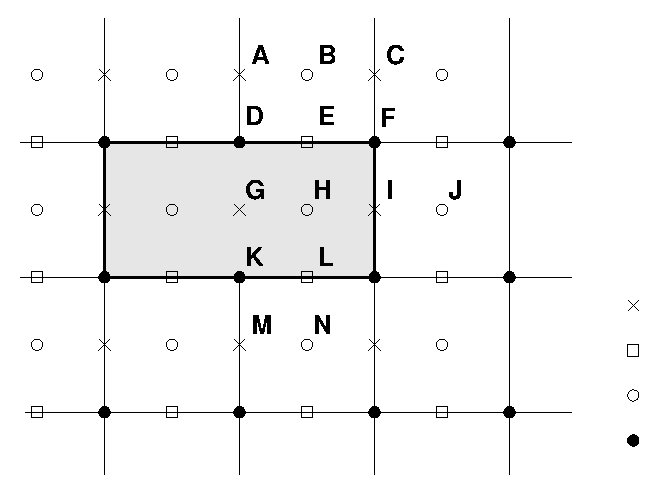
\includegraphics{pics/mask2}%
\end{picture}%
\begin{picture}(348,263)(92,465)
\put(490,552){\makebox(0,0)[lb]{-- $u$ points}}
\put(490,528){\makebox(0,0)[lb]{-- $v$ points}}
\put(490,504){\makebox(0,0)[lb]{-- $\rho$ points}}
\put(490,480){\makebox(0,0)[lb]{-- $\psi$ points}}
\end{picture}
\caption{Masked region within the domain}
\label{fmask1}
\end{figure}

\subsubsection{Velocity}
At the end of every time step, the values of many variables within the
masked region are set to zero by multiplying by the mask for either the
$u$, $v$ or $\rho$ points.  This is appropriate for the $v$ points {\bf
E} and {\bf L} in Fig.\ \ref{fmask1}, since the flow in and out of the
land should be zero.  It is likewise appropriate for the $u$ point at
{\bf I}, but is not necessarily correct for point {\bf G}.  The only
term in the $u$ equation that requires the $u$ value at point {\bf G}
is the horizontal viscosity, which has a term of the form
$\frac{\partial}{\partial \eta} \nu \frac{\partial u}{\partial \eta}$.
Since point {\bf G} is used in this term by both points {\bf A} and
{\bf M}, it is not sufficient to replace its value with that of the
image point for {\bf A}.  Instead, the term $\frac{\partial u}{\partial
\eta}$ is computed and the values at points {\bf D} and {\bf K} are
replaced with the values appropriate for either free-slip or no-slip
boundary conditions.  Likewise, the term $\frac{\partial}{\partial \xi}
\nu \frac{\partial v}{\partial \xi}$ in the $v$ equation must be corrected
at the mask boundaries.

This is accomplished by having a fourth mask array defined at the $\psi$
points, in which the values are set to be no-slip in \code{metrics}.
For no-slip boundaries, we count on the values inside
the land (point {\bf G}) having been zeroed out.  For point {\bf D}, the
image point at {\bf G} should contain minus the value of $u$ at point
{\bf A}.  The desired value of $\frac{\partial u}{\partial \eta}$ is
therefore $2 u_{\bf A}$ while instead we have simply $u_{\bf A}$.
In order to achieve the correct result, we multiply by a mask which
contains the value 2 at point {\bf D}.  It also contains a 2 at point
{\bf K} so that $\frac{\partial u}{\partial \eta}$ there will acquire
the desired value of $-2 u_{\bf M}$. The corner point {\bf F} is set to
have a value of 1.

\subsubsection{Temperature, salinity and surface elevation}

The handling of masks by the temperature, salinity and surface
elevation equations is similar to that in the momentum equations, and
is in fact simpler.  Values of $T$, $S$ and $\zeta$ inside the land
masks, such as point {\bf H} in Fig.\ \ref{fmask1}, are set to zero
after every time step.  This point would be used by the horizontal
diffusion term for points {\bf B}, {\bf J}, and {\bf N}.  This is
corrected by setting the first derivative terms at points {\bf E}, {\bf
I}, and {\bf L} to zero, to be consistent with a no-flux boundary
condition.
Note that the equation of state must be able to handle $T = S = 0$
since this is the value inside masked regions.

%\subsubsection{Free surface and pressure gradients}

%The surface elevation inside the land mask is simply used for setting
%the total depth and therefore the location of the $s$-coordinate
%surfaces.

\subsubsection{Wetting and drying}

There is now an option to have wetting and drying in the model, in
which a cell can switch between being wet or being dry as the tides
come in and go out, for instance. Cells which are masked out as in
Fig.~\ref{fmask1} are never allowed to be wet, however.
\begin{itemize}
   \item In the case of wetting and drying, a critical depth, $D_{crit}$,
is supplied by the user.
   \item The total water depth ($D=h+\zeta$) is compared to $D_{crit}$.
If the water level is less than this depth, no flux is allowed out
of that cell. Water can always flow in and resubmerge the cell.
  \item The wetting and drying only happens during the 2-D
computations; the 3-D computations see a depth of
$D_{crit}$ in the ``dry'' areas.
  \item The ice component now checks for dry cells when computing
the ice rheology.
\end{itemize}

\subsection{Time-stepping overview}

While time stepping the model, we have a stored history of the model fields
at time $n-1$, an estimate of the fields at the current time $n$, and
we need to come up with an estimate for time $n+1$. For reasons of
efficiency, we choose to use a split-explicit time step, integrating
the depth-integrated equations with a shorter time step than the full
3-D equations. There is an integer ratio $M$ between the time steps. The
exact details of how the time stepping is done vary from one version
of ROMS to the next, with the east coast ROMS described here being older
than other branches. Still, all versions have these steps:

\begin{enumerate}
  \item Take a predictor step for at least the 3-D tracers to time
  $n+\frac{1}{2}$.
  \item Compute $\overline{\rho}$ and
$\rho^*$ for use in the depth-integrated time steps, from the density
either at time $n$ or time $n+\frac{1}{2}$.
  \item Depth integrate the 3-D momentum right-hand side terms at
time $n+\frac{1}{2}$ for use in the depth-integrated time steps (or extrapolate
to obtain an estimate of those terms).
  \item Take all the depth-integrated steps. Store weighted
time-means of the $\overline{u}$, $\overline{v}$ fields centered at both
time $n+\frac{1}{2}$ and time $n+1$ (plus $\zeta$ at time $n+1$). The latter
requires this time stepping to extend past time $n+1$, using $M^*$ steps
rather than just $M$.
  \item Use the weighted time-means from depth-integrated fields to
complete the corrector step for the 3-D fields to time $n+1$.
\end{enumerate}
Great care is taken to avoid the introduction of a mode-splitting
instability due to the use of shorter time steps for the depth-integrated
computations.

The mode coupling has evolved through the various ROMS versions,
as shown in Fig.~\ref{ftimestep1} (from \cite{SS2008a}). The time stepping
schemes are also listed in Table~\ref{ttimestep1} and described in
detail in \cite{SS2005} and \cite{SS2008b}; the relevant ones
are described in Appendix~\ref{Frog}.

\begin{figure}[p]
\setlength{\unitlength}{1.0in}%
%
\begin{picture}(6.5,7.5)(0,0)
  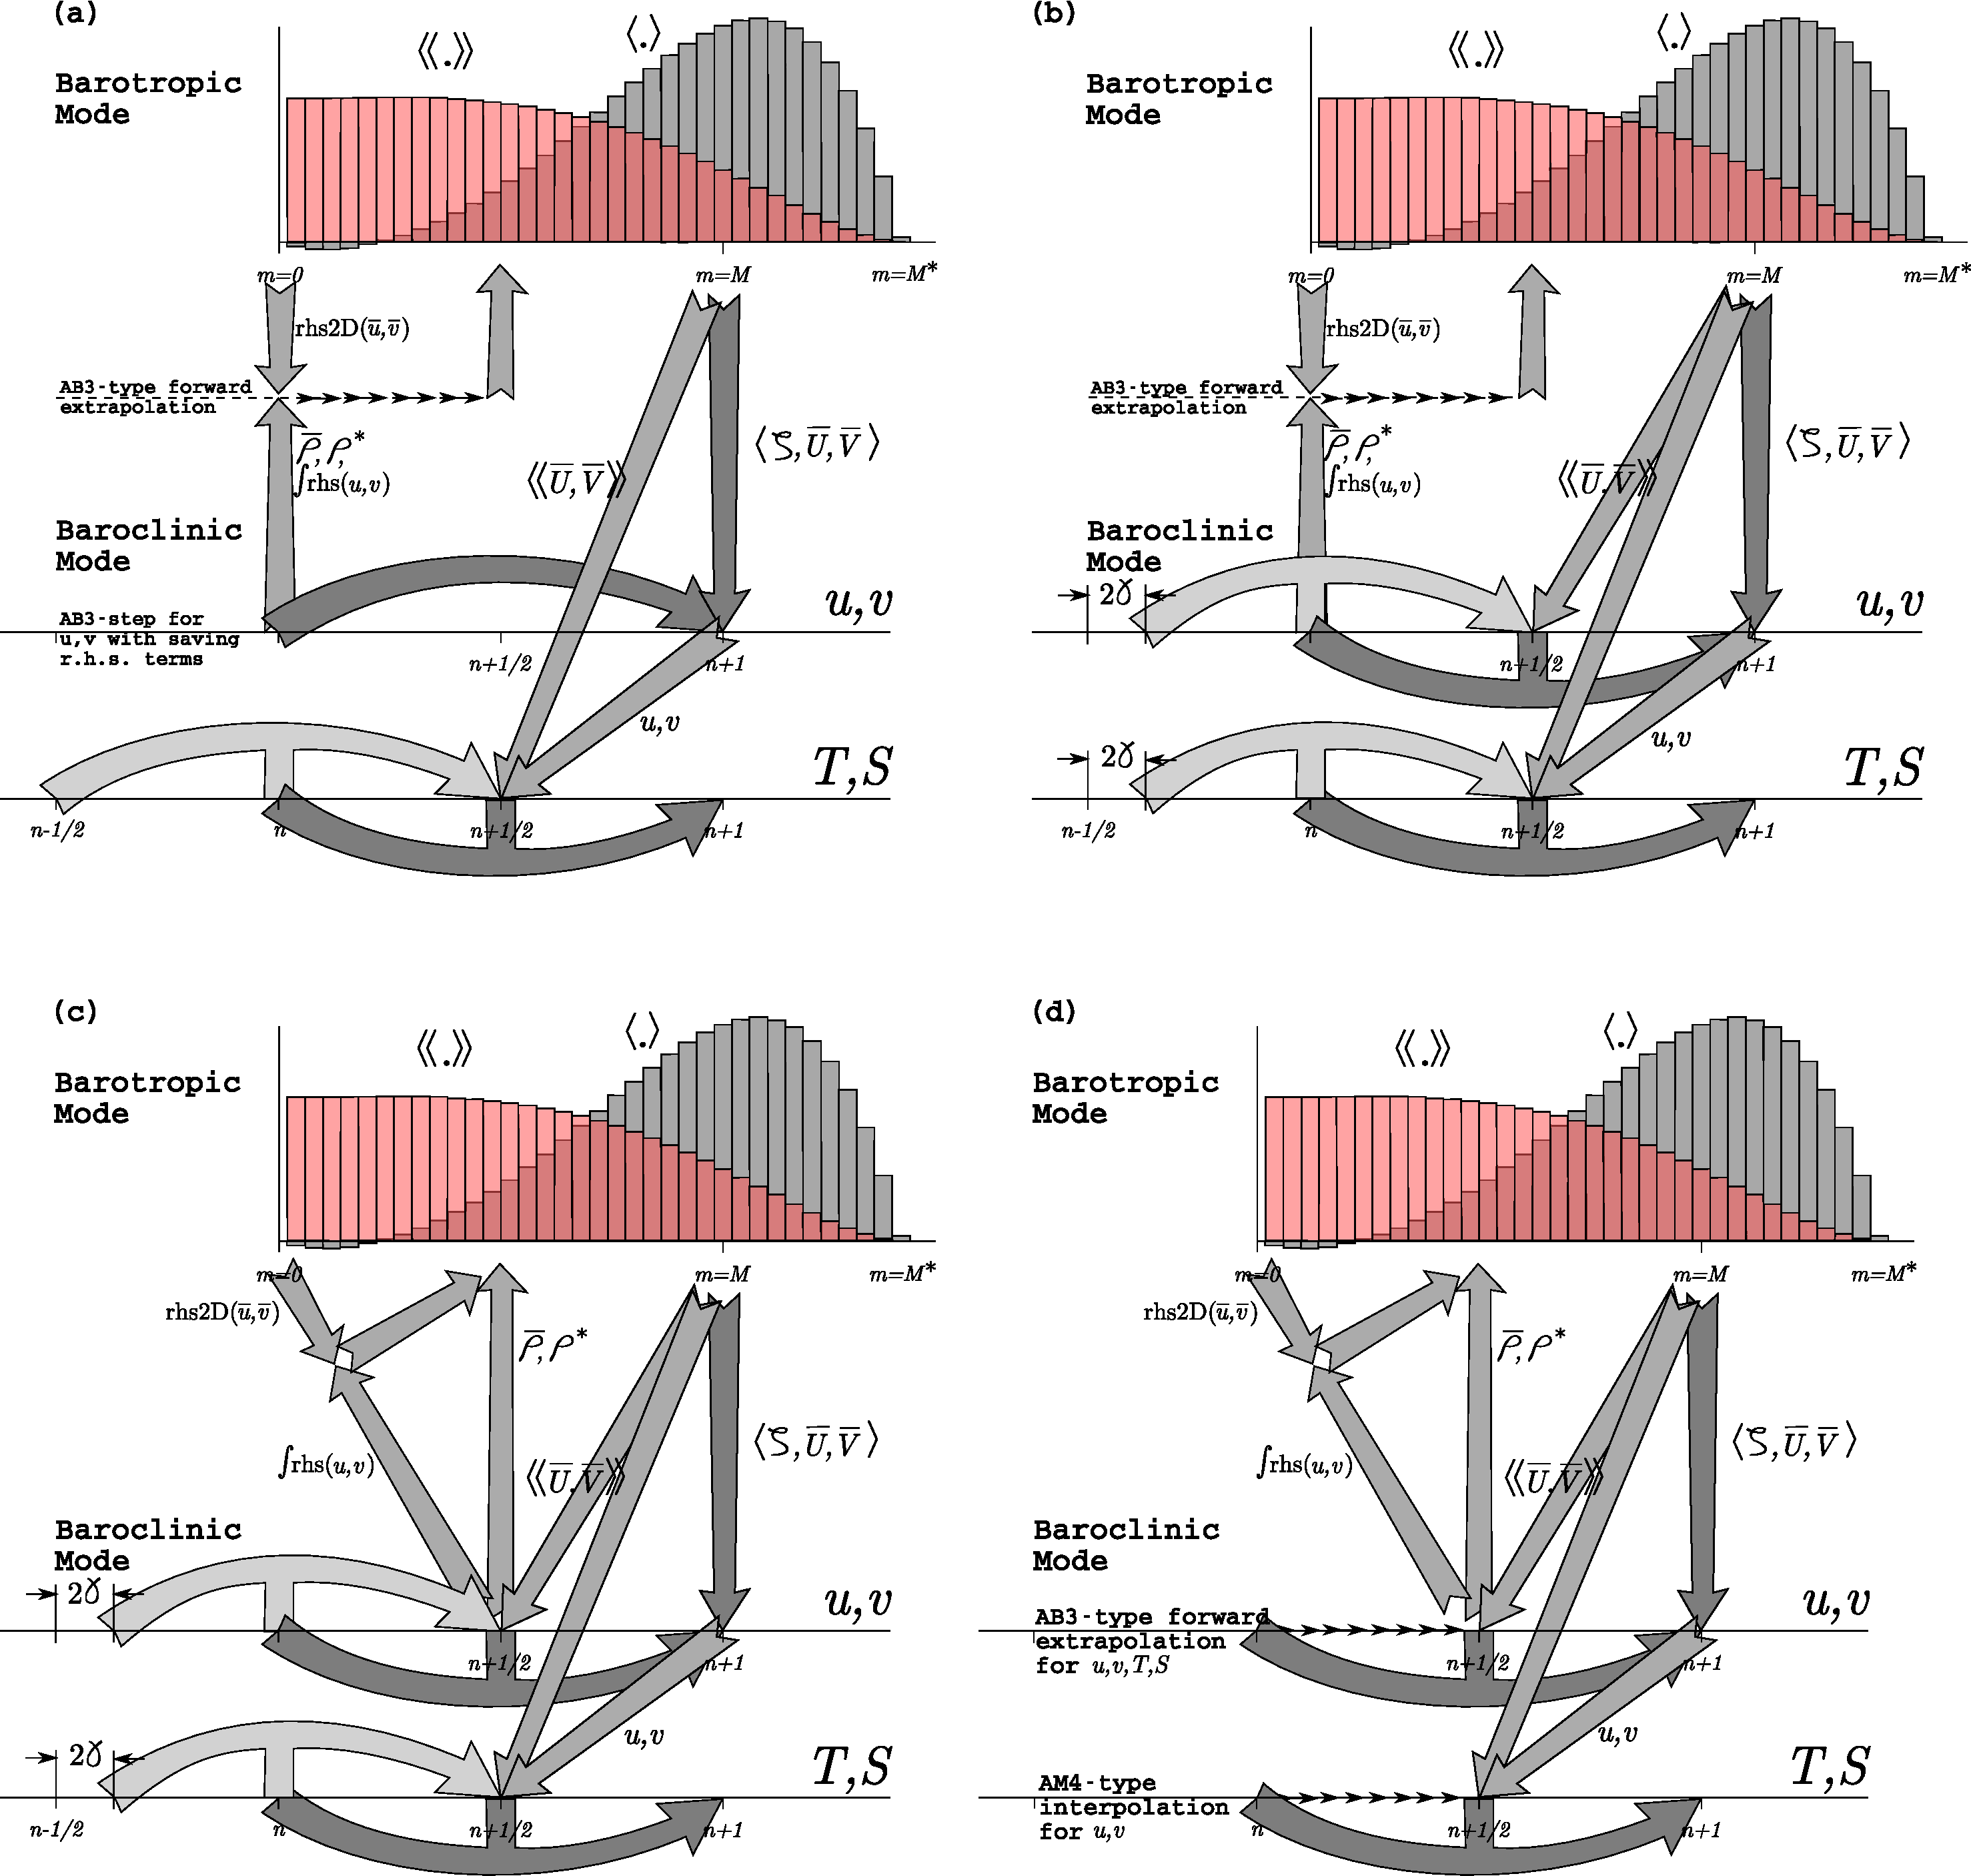
\includegraphics[width=6.5in]{pics/timestep_all}%
\end{picture}%
\caption{Diagrams of the time stepping and mode coupling used in
various ROMS versions. (a) Rutgers University ROMS (from
myroms.org), (b) ROMS AGRIF, (c) UCLA ROMS, described in \cite{SS2005},
(d) non-hydrostatic ROMS (\cite{Kanarska2007}). In all, the curved
arrows update the 3-D fields; those with ``pillars'' are leapfrog
in nature with the pillar representing the r.h.s. terms. Straight
arrows indicate exchange between the barotropic and baroclinic
modes. The shape functions for the fast time steps show just one
option out of many possibilities. The grey function has weights to
produce an estimate at time $n+1$, while the light red function has
weights to produce an estimate at time $n+\frac{1}{2}$.}
 \label{ftimestep1}
\end{figure}

\begin{table}[thb]
 \centerline{
\begin{tabular}{|l|c|c|c|c|c|} \hline
  & SCRUM 3.0 & Rutgers & AGRIF & UCLA & Non-hydrostatic \\
  \hline
  Reference & \cite{Hedstrom2000} & \cite{DAMEE_1} &
  \cite{Penven2006} & \cite{SS2005} & \cite{Kanarska2007} \\
  \hline
  Barotropic  & LF-TR & LF-AM3 with
  & LF-AM3 with & Gen. FB & Gen. FB \\
  mode & & FB feedback & FB feedback\footnote{The generalized FB
  barotropic mode was ported into the newest AGRIF code at the end
  of 2007.} & (AB3-AM4) & (AB3-AM4) \\
  \hline
  2-D $\alpha_{\max}$, iter. & $\sqrt{2}$,
  (2)\footnote{The number in parentheses (e.g., 2) indicates the
  number of r.h.s. computations per time step. If there are two
  parenthesized number, the first one is for momenta, the second for
  tracers.} & 1.85, (2) & 1.85,
  (2) & 1.78, (1) & 1.78, (1) \\
  \hline
  3-D momenta & AB3 & AB3 & LF-AM3 & LF-AM3 & AB3 (mod) \\
  \hline
  Tracers & AB3 & LF-TR & LF-AM3 & LF-AM3 & AB3 (mod) \\
  \hline
  Internal & AB3 & Gen.\ FB &
  LF-AM3, & LF-AM3, &
  Gen.\ FB \\
  waves & & (AB3-TR) & FB feedback & FB feedback & (AB3-AM4) \\
  \hline
  $\alpha_{\max}$, advect. & 0.72 & 0.72 & 1.587 &
  1.587 & 0.78 \\
  \hline
  $\alpha_{\max}$, Cor. & 0.72 & 0.72 & 1.587 &
  1.587 & 0.78 \\
  \hline
  $\alpha_{\max}$, int. w. & 0.72, (1) & 1.14,
  (1,2) & 1.85, (2) &
  1.85, (2) & 1.78, (1) \\
  \hline
  \end{tabular}
  }
\label{ttimestep1}
\caption{The time stepping schemes used in the various ROMS versions.
$\alpha \equiv \omega \delta t$ is the Courant number and $\omega=ck$
is the frequency for a wave component with wavenumber $k$.}
\end{table}

\subsection{Conservation properties}
\label{Enrg}
From Shchepetkin and McWilliams (2005) \cite{SS2005}, we have a
tracer concentration equation in advective form:
\begin{equation}
  \frac{\partial C}{\partial t} + (u \cdot \nabla) C = 0
  \label{eqt1}
\end{equation}
and also a tracer concentration equation in conservation form:
\begin{equation}
   \frac{\partial C}{\partial t} + \nabla \cdot (u C) = 0.
  \label{eqt2}
\end{equation}
The continuity equation:
\begin{equation}
   ( \nabla \cdot u) = 0
\end{equation}
can be used to get from one tracer equation to the other.
As a consequence of eq.~(\ref{eqt1}), if the tracer is spatially
uniform, it will remain so regardless of the velocity field
(constancy preservation). On the other hand, as a consequence of
(\ref{eqt2}), the volume integral of the tracer concentration is conserved
in the absence of internal sources and fluxes through the boundary. Both
properties are valuable and should be retained when constructing numerical
ocean models.

The semi-discrete form of the tracer equation
(\ref{st15}) is:
\begin{equation}
   \frac{\partial}{\partial t} \left( \frac{H_z C}{m n} \right)
   + \delta_{\xi} \left(
   \frac{u \overline{H_z}^\xi \overline{C}^\xi }{\overline{n}^\xi} \right)
   + \delta_{\eta} \left(
   \frac{v \overline{H_z}^\eta \overline{C}^\eta }{\overline{m}^\eta} \right)
   + \delta_\sigma \left( \overline{C}^\sigma
   \frac{H_z \Omega}{m n} \right) =
\\ \vspace{2mm}
   \frac{ 1}{mn} \frac{\partial}{\partial \sigma}
   \left( \frac{K_m}{\Delta z} \frac{\partial C}{\partial \sigma} \right) +
   {\cal D}_C + {\cal F}_C
\label{tfull}
\end{equation}
Here $\delta_{\xi}$, $\delta_{\eta}$ and $\delta_\sigma$ denote simple
centered finite-difference approximations to $\partial / \partial \xi$,
$\partial / \partial \eta$ and $\partial / \partial \sigma$ with the
differences taken over the distances $\Delta\xi$, $\Delta\eta$ and
$\Delta \sigma$, respectively. $\Delta z$ is the vertical distance from one
$\rho$ point to another. $\overline{ ( \hspace{5mm} )}^{\xi}$,
$\overline{ ( \hspace{5mm} )}^{\eta}$ and $\overline{ ( \hspace{5mm}
)}^\sigma$ represent averages taken over the distances $\Delta\xi$, $\Delta
\eta$ and $\Delta \sigma$. % $I_\sigma^0$ indicates a second-order vertical
%integral computed as a sum from level $\sigma$ to the surface at
%$\sigma=0$.

The finite volume version of the same equation is no different,
except that a quantity $C$ is defined as the volume-averaged
concentration over the grid box $\Delta V$:
\begin{equation}
   C = \frac{mn}{H_z} \int_{\Delta V} \frac{H_z C}{mn} \delta \xi
   \, \delta \eta \, \delta \sigma
\end{equation}
The quantity  $\left(
\frac{u \overline{H_z}^\xi \overline{C}^\xi}{\overline{n}^\xi} \right)$
is the flux through an interface between adjacent grid boxes.

This method of averaging was chosen because it internally conserves
first moments in the model domain, although it is still possible to
exchange mass and energy through the open boundaries. The method is
similar to that used in Arakawa and Lamb \cite{AL}; though their
scheme also conserves enstrophy. Instead, we will focus on (nearly) retaining
constancy preservation while coupling the barotropic
(depth-integrated) equations and the baroclinic equations.

The time step in eq.~(\ref{tfull}) is assumed to be from time $n$ to
time $n+1$, with the other terms being evaluated at time
$n+\frac{1}{2}$ for second-order accuracy.
Setting $C$ to 1 everywhere reduces eq.~(\ref{tfull}) to:
\begin{equation}
   \frac{\partial}{\partial t} \left( \frac{H_z}{m n} \right)
   + \delta_{\xi} \left(
   \frac{u \overline{H_z}^\xi }{\overline{n}^\xi} \right)
   + \delta_{\eta} \left(
   \frac{v \overline{H_z}^\eta}{\overline{m}^\eta} \right)
   + \delta_\sigma \left( 
   \frac{H_z \Omega}{m n} \right) = 0
\label{contfull}
\end{equation}
If this equation holds true for the step from time $n$ to time $n+1$, then
our constancy preservation will hold.

In a hydrostatic model such as ROMS, the discrete continuity
equation is needed to compute vertical velocity rather than grid-box
volume $\frac{H_z}{m n}$ (the latter is controlled by changes in
$\zeta$ in the barotropic mode computations). Here, $\frac{H_z
\Omega}{m n}$ is the finite-volume flux across the {\em moving}
grid-box interface, vertically on the $w$ grid.

The vertical integral of the continuity eq.~(\ref{st17}), using
the vertical boundary conditions on $\Omega$, is:
\begin{equation}
   \frac{\partial}{\partial t} \left( \frac{\zeta}{mn} \right) +
   \delta_{\xi} \left(
   \frac{\overline{u} \overline{D}^\xi }{\overline{n}^\xi} \right)
   + \delta_{\eta} \left(
   \frac{\overline{v} \overline{D}^\eta}{\overline{m}^\eta} \right)
   = 0
\label{zeta1}
\end{equation}
where $\zeta$ is the surface elevation, $D= h+\zeta$ is the total
depth, and $\overline{u},\overline{v}$ are the depth-integrated
horizontal velocities. This equation and the corresponding 2-D
momentum equations are time stepped on a shorter time step than 
eq.~(\ref{tfull}) and the other 3-D equations. Due to the details in
the mode coupling, it is only possible to maintain constancy
preservation to the accuracy of the barotropic time steps.

\subsection{Depth-integrated equations}
\label{Vort}
The depth average of a quantity $A$ is given by:
\begin{equation}
   \overline{A} = \frac{1}{D} \int_{-1}^0 H_z A d\sigma
\end{equation}
where the overbar indicates a vertically averaged quantity and
\begin{equation}
   D \equiv \zeta(\xi, \eta, t) + h(\xi, \eta)
\end{equation}
is the total depth of the water column.  The vertical integral of
equation (\ref{st13}) is:
%{\samepage
\begin{multline}
   \frac{\partial}{\partial t} \left( \frac{D \overline{u}}{mn} \right)
   + \frac 
   {\partial}{\partial \xi} \left( \frac{D \overline{uu}}{n} \right )
   + \frac 
   {\partial}{\partial \eta} \left( \frac{D \overline{uv}}{m} \right)
   - \frac{Df\overline{v}}{mn}
\\ \vspace{1mm}
   - \left[ \overline{vv}
   \frac{\partial}{\partial \xi}
   \left( \frac{1}{n} \right) - \overline{uv}
   \frac{\partial}{\partial \eta} \left(
   \frac{1}{m} \right) \right] D = 
   - \frac{D}{n}
   \left( \frac{\partial \overline{\phi_2}}{\partial \xi} +
   g \frac{\partial \zeta}{\partial \xi} \right)
\\ \vspace{1mm}
   + \frac{ D}{mn}
   \left( \overline{\cal F}_u + \overline{\cal D}_{h_u} \right) 
   + \frac{1}{mn} \left( \tau^{\xi}_s - \tau^{\xi}_b \right)
\label{ubar1}
\end{multline}
%}
where $\phi_2$ includes the $\frac{\partial z}{\partial \xi}$ term,
$\overline{\cal D}_{h_u}$ is the horizontal viscosity, and the
vertical viscosity only contributes through the upper and lower
boundary conditions.  The corresponding vertical integral of equation
(\ref{st14}) is:
%{\samepage
\begin{multline}
   \frac{\partial}{\partial t} \left( \frac{D \overline{v}}{mn} \right)
   + \frac 
   {\partial}{\partial \xi} \left( \frac{D \overline{uv}}{n} \right )
   + \frac 
   {\partial}{\partial \eta} \left( \frac{D \overline{vv}}{m} \right)
   + \frac{Df\overline{u}}{mn}
\\ \vspace{1mm}
   + \left[ \overline{uv}
   \frac{\partial}{\partial \xi}
   \left( \frac{1}{n} \right) - \overline{uu}
   \frac{\partial}{\partial \eta} \left(
   \frac{1}{m} \right) \right] D = 
   - \frac{D}{m}
   \left( \frac{\partial \overline{\phi_2}}{\partial \eta} +
   g \frac{\partial \zeta}{\partial \eta} \right)
\\ \vspace{1mm}
   + \frac{ D}{mn}
   \left( \overline{\cal F}_v + \overline{\cal D}_{h_v} \right) 
   + \frac{1}{mn} \left( \tau^{\eta}_s - \tau^{\eta}_b \right) .
\label{vbar1}
\end{multline}
%}
We also need the vertical integral of equation (\ref{st17}), shown
above as eq.~ (\ref{zeta1}).

The presence of a free surface introduces waves which propagate at a
speed of $\sqrt{gh}$.  These waves usually impose a more severe
time-step limit than any of the internal processes.  We have therefore
chosen to solve the full equations by means of a split time step.  In
other words, the depth integrated equations (\ref{ubar1}),
(\ref{vbar1}), and (\ref{zeta1}) are integrated using a short time step
and the values of $\overline{u}$ and $\overline{v}$ are used
to replace those found by integrating the full equations on a longer
time step.  A diagram of the barotropic time stepping is shown in
Fig.~\ref{ftspl}.
\begin{figure}[htb]
\setlength{\unitlength}{1.00in}%
%
\begin{picture}(5,2)(0,0.3)%
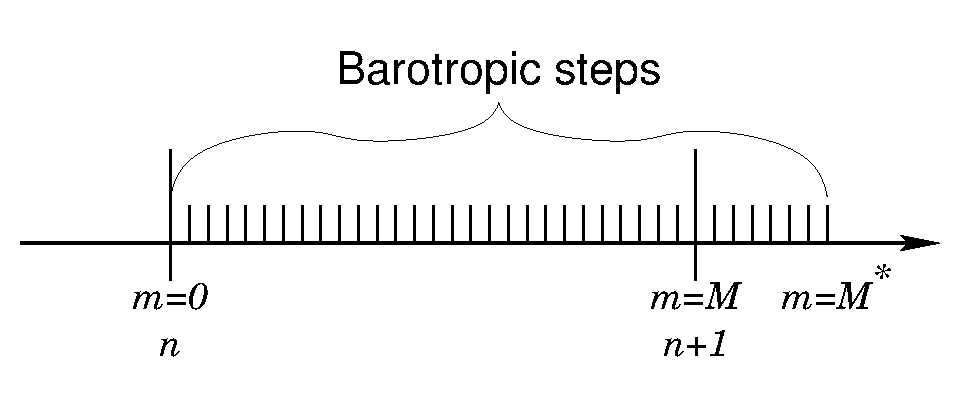
\includegraphics{pics/shortstep}%
\end{picture}%
 
 \caption{The split time stepping used in the model.}
 \label{ftspl}
\end{figure}

Some of the terms in equations (\ref{ubar1}) and (\ref{vbar1}) are
updated on the short time step while others are not.  The contributions
from the slow terms are computed once per long time step and stored.  If
we call these terms $R_{u_{\rm slow}}$ and $R_{v_{\rm slow}}$, equations
(\ref{ubar1}) and (\ref{vbar1}) become:
%{\samepage
\begin{multline}
   \frac{\partial}{\partial t} \left( \frac{D \overline{u}}{mn} \right)
   + \frac{\partial}{\partial \xi}
   \left( \frac{D \overline{u}\,\overline{u}}{n} \right)
   + \frac{\partial}{\partial \eta}
   \left( \frac{D \overline{u}\,\overline{v}}{m} \right)
   - \frac{Df\overline{v}}{mn}
\\ \vspace{1mm}
   - \left[ \overline{v}\,\overline{v}
   \frac{\partial}{\partial \xi}
   \left( \frac{1}{n} \right) - \overline{u}\,\overline{v}
   \frac{\partial}{\partial \eta} \left(
   \frac{1}{m} \right) \right] D = R_{u_{\rm slow}} -
   \frac{gD}{n} \frac{\partial \zeta}{\partial \xi}
    + \frac{D}{mn} {\cal D}_{\overline{u}}
   - \frac{1}{mn} \tau^{\xi}_b
\label{ubar2}
\end{multline}
%}  
%{\samepage
\begin{multline}
   \frac{\partial}{\partial t} \left( \frac{D \overline{v}}{mn} \right)
   + \frac{\partial}{\partial \xi}
   \left( \frac{D \overline{u}\,\overline{v}}{n} \right)
   + \frac{\partial}{\partial \eta}
   \left( \frac{D \overline{v}\,\overline{v}}{m} \right)
   + \frac{Df\overline{u}}{mn}
\\ \vspace{1mm}
   + \left[ \overline{u}\,\overline{v}
   \frac{\partial}{\partial \xi}
   \left( \frac{1}{n} \right) - \overline{u}\,\overline{u}
   \frac{\partial}{\partial \eta} \left(
   \frac{1}{m} \right) \right] D = R_{v_{\rm slow}} -
   \frac{gD}{m} \frac{\partial \zeta}{\partial \eta}
    + \frac{ D}{mn} {\cal D}_{\overline{v}}
   - \frac{1}{mn} \tau^{\eta}_b .
\label{vbar2}
\end{multline}
%}
When time stepping the model, we compute the right-hand-sides for
equations (\ref{st13}) and (\ref{st14}) as well as the
right-hand-sides for equations (\ref{ubar2}) and (\ref{vbar2}).  The
vertical integral of the 3-D right-hand-sides are obtained and then the
2-D right-hand-sides are subtracted.  The resulting fields are the slow
forcings $R_{u_{\rm slow}}$ and $R_{v_{\rm slow}}$.  This was found to
be the easiest way to retain the baroclinic contributions of the
non-linear terms such as $\overline{uu} - \overline{u}\,\overline{u}$.

The model is time stepped from time $n$ to time $n+1$ by using short
time steps on equations (\ref{ubar2}), (\ref{vbar2}) and (\ref{zeta1}).
Equation (\ref{zeta1}) is time stepped first, so that an estimate of the
new $D$ is available for the time rate of change terms
in equations (\ref{ubar2}) and (\ref{vbar2}).
A third-order predictor-corrector time stepping is used.
In practice, we actually time step all the way to time
$(n+\code{dtfast} \times M^\star)$,
while maintaining weighted averages of the values of $\overline{u}$,
$\overline{v}$ and $\zeta$.  The averages are used to replace the
values at time $n+1$ in both the baroclinic and barotropic modes,
and for recomputing the vertical grid spacing $H_z$.
Fig.~\ref{fbarostep1} shows one option for how these weights might look.

\begin{figure}[tbp]
\setlength{\unitlength}{1.in}%
\begin{picture}(6.5,6.5)(0,0)
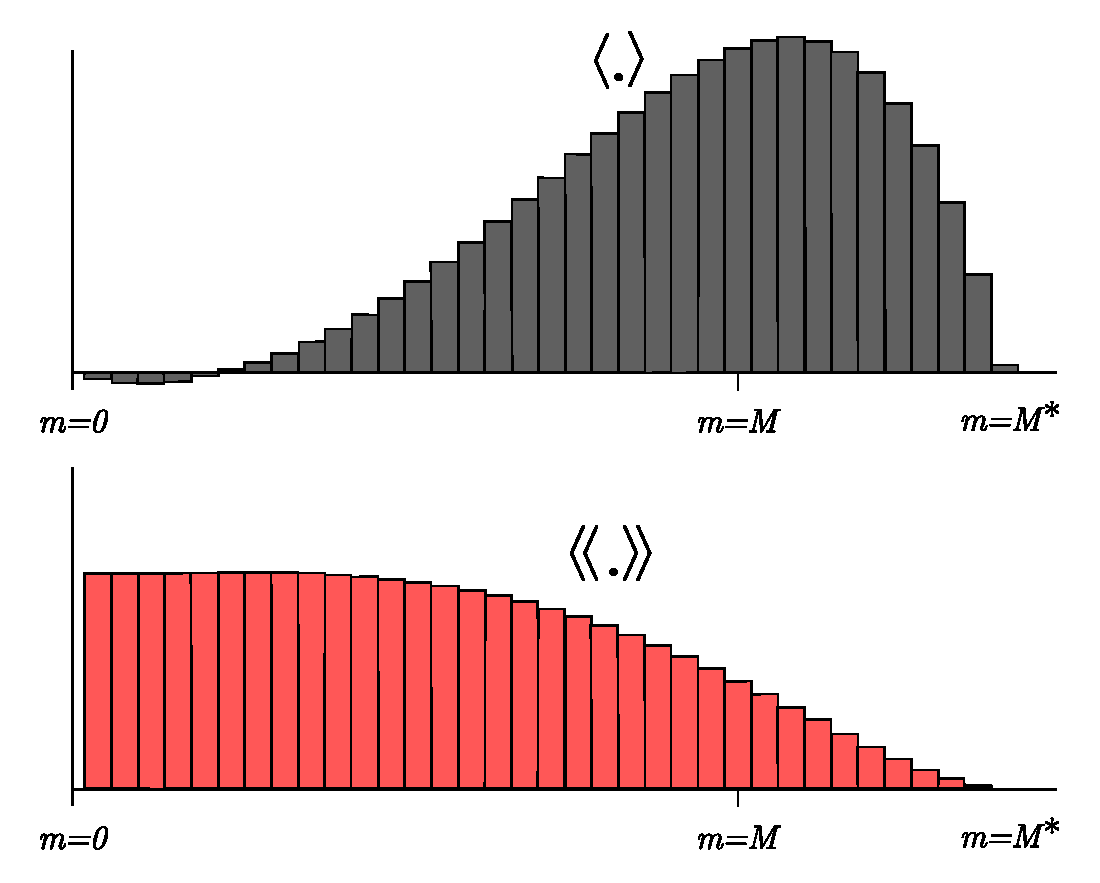
\includegraphics[width=6.5in]{pics/barostep}%
\end{picture}%
\caption{Weights for the barotropic time stepping. The upper panel
shows the primary weights, centered at time $n+1$, while the lower panel shows
the secondary weights weights, centered at time $n+\frac{1}{2}$.}
\label{fbarostep1}
\end{figure}

The primary weights, $a_m$, are used to compute $\langle \zeta
\rangle^{n+1} \equiv \sum_{m=1}^{M^\star} a_m \zeta^m$. There is a
related set of secondary weights $b_m$, used as $\langle \! \langle
\overline{u} \rangle \! \rangle^{n+\frac{1}{2}} \equiv \sum_{m=1}^{M^\star} b_m
\overline{u}^m$. In order to maintain constancy preservation, this
relation must hold:
\begin{equation}
  \langle \zeta \rangle_{i,j}^{n+1} = \langle \zeta \rangle_{i,j}^n -
  (mn)_{i,j} \Delta t \left[ \left\langle \!\! \left\langle
  \frac{D\overline u}{n} \right\rangle \!\!
  \right\rangle_{i+\frac{1}{2},j}^{n+\frac{1}{2}}
  - \left\langle \!\! \left\langle \frac{D\overline u}{n} \right\rangle
  \!\! \right\rangle_{i-\frac{1}{2},j}^{n+\frac{1}{2}} +
  \left\langle \!\! \left\langle
  \frac{D\overline v}{m} \right\rangle \!\!
  \right\rangle_{i,j+\frac{1}{2}}^{n+\frac{1}{2}}
  - \left\langle \!\! \left\langle \frac{D\overline v}{m} \right\rangle
  \!\! \right\rangle_{i,j-\frac{1}{2}}^{n+\frac{1}{2}} \right]
\label{zeta3}
\end{equation}
Shchepetkin and McWilliams (\cite{SS2005}) introduce a range of
possible weights, but the ones used here have a shape function:
\begin{equation}
   A(\tau) = A_0 \left\{ \left( \frac{\tau}{\tau_0} \right)^p \left[ 1-
   \left(\frac{\tau}{\tau_0} \right)^q \right] - r \frac{\tau}{\tau_0}
   \right\}
\label{weights}
\end{equation}
where $p, q$ are parameters and $A_0, \tau_0$, and $r$ are chosen to
satisfy normalization, consistency, and second-order accuracy
conditions,
\begin{equation}
   I_n = \int_0^{\tau^\star} \tau^n A(\tau) d \tau = 1, \quad n=0,1,2
\label{second}
\end{equation}
using Newton iterations. $\tau^\star$ is the upper limit of $\tau$
with $A(\tau) \geq 0$. In practice we initially set
$$
  A_0 = 1, r = 0 \quad \mbox{and} \quad
  \tau = \frac{(p+2)(p+q+2)}{(p+1)(p+q+1)},
$$
compute $A(\tau)$ using eq.~(\ref{weights}), normalize using:
\begin{equation}
   \sum_{m=1}^{M^\star} a_m \equiv 1, \quad
   \sum_{m=1}^{M^\star} a_m\frac{m}{M} \equiv 1,
\end{equation}
and adjust $r$ iteratively to satisfy the $n=2$ condition of
(\ref{second}). We are using values of $p=2$, $q=4$, and $r=0.284$.
This form allows some negative weights for small $m$, allowing
$M^\star$ to be less than $1.5M$.

ROMS also supports an older cosine weighting option, which isn't
recommended since it is only first-order accurate.

\subsection{Density in the mode coupling}

Equation (\ref{ubar2}) contains the term $R_{u_{\rm slow}}$,
computed as the difference between the 3-D right-hand-side and the
2-D right-hand-side. The pressure gradient therefore has the form:
\begin{equation}
   -\frac{g D}{n} \frac{\partial \zeta}{\partial \xi} +
   \left[\frac{g D}{n} \frac{\partial \zeta}{\partial \xi} + {\cal F}
   \right]
\end{equation}
where the term in square brackets is the mode coupling term and is
held fixed over all the barotropic steps and
\begin{equation}
  {\cal F} = - \frac{1}{\rho_0 n} \int_{-h}^\zeta \frac{\partial
  P}{\partial \xi} dz
\end{equation}
is the vertically integrated pressure gradient. The latter is a function
of the bathymetry, free surface gradient, and the free surface itself,
as well as the vertical distribution of density.

The disadvantage of this approach is that after the barotropic time
stepping is complete and the new free surface is substituted into
the full baroclinic pressure gradient, its vertical integral will
no longer be equal to the sum of the new surface slope term and the
original coupling term based on the old free surface. This is one
form of mode-splitting error which can lead to trouble because the
vertically integrated pressure gradient is not in balance with the
barotropic mass flux.

Instead, let us define the following:
\begin{equation}
  \overline{\rho} = \frac{1}{D} \int_{-h}^\zeta \rho dz , \quad
  \rho^\star = \frac{1}{\frac{1}{2} D^2} \int_{-h}^\zeta
  \left\{ \int_z^\zeta \rho dz^{\prime} \right\} dz
\end{equation}
Changing the vertical coordinate to $\sigma$ yields:
\begin{equation}
  \overline{\rho} =  \int_{-1}^0 \rho d\sigma , \quad
  \rho^\star = 2 \int_{-1}^0
  \left\{ \int_\sigma^0 \rho d\sigma^{\prime} \right\} d\sigma
\end{equation}
which implies that $\overline{\rho}$ and $\rho^\star$ are actually
independent of $\zeta$ as long as the density profile $\rho =
\rho(\sigma)$ does not change. The vertically integrated pressure
gradient becomes:
\begin{equation}
   -\frac{1}{\rho_0} \frac{g}{n} \left\{ \frac{\partial}{\partial \xi}
   \left( \frac{\rho^\star D^2}{2} \right) - \overline{\rho} D
   \frac{\partial h}{\partial \xi} \right\} = -\frac{1}{\rho_0}
   \frac{g}{n} D \left\{ \rho^\star \frac{\partial \zeta}{\partial \xi} +
   \frac{D}{2} \frac{\partial \rho^\star}{\partial \xi} + (\rho^\star -
   \overline{\rho}) \frac{\partial h}{\partial \xi} \right\}
\end{equation}
In the case of uniform density $\rho_0$, we obtain $\rho^\star \equiv
\overline{\rho} \equiv \rho_0$, but we otherwise have two new terms.
The accuracy of these terms depends on an accurate vertical
integration of the density, as described in Shchepetkin and
McWilliams (2005, \cite{SS2005}).

\subsection{Time stepping: internal velocity modes and tracers}
The momentum equations (\ref{st13}) and(\ref{st14}) are advanced before
the tracer equation, by computing all the terms except the vertical
viscosity and then using the implicit scheme described in \S\ref{Vfric}
to find the new values for $u$ and $v$. The depth-averaged component
is then removed and replaced by the $\langle \overline{u} \rangle$
and $\langle \overline{v} \rangle$ computed as in \S\ref{Vort}.
A third-order Adams-Bashforth (AB3) time stepping is used, requiring
multiple right-hand-side time levels (see Appendix~\ref{Frog}). These
stored up r.h.s. values can be used to extrapolate to a value at
time $n+\frac{1}{2}$ for use in the barotropic steps as shown in
Fig.~\ref{ftimestep1}.

The tracer concentration equation (\ref{tfull}) is advanced in a
predictor-corrector leapfrog-trapezoidal step, with great care taken to
optimize both the conservation and constancy-preserving properties of the
continuous equations. The corrector step can maintain both, as long as it
uses velocities and column depths which satisfy eq.~(\ref{zeta3}). This
also requires tracer values centered at time $n+\frac{1}{2}$, obtained
from the predictor step. The vertical diffusion is computed as in
\S\ref{Vfric}.

The predictor step cannot be both constancy-preserving and conservative; it
was therefore decided to make it constancy-preserving. Also, since it is
only being used to compute the advection for the corrector step, the
expensive diffusion operations are not carried out during the predictor step.

The preceeding notes on tracer advection refer to all but the MPDATA
option. The MPDATA algorithm has its own predictor-corrector with
emphasis on not allowing values to exceed their original range;
it therefore gives up the constancy-preservation. This is most
noticeable in shallow areas with large tides.

\subsection{Advection schemes}
\label{Advect}
The advection of a tracer $C$ has an equation of the form
\begin{equation}
  \frac{\partial}{\partial t} \frac{ H_z C}{mn} =
  - \frac{\partial}{\partial \xi} F^\xi
  - \frac{\partial}{\partial \eta} F^\eta
  - \frac{\partial}{\partial \sigma} F^\sigma ,
\end{equation}
where we have introduced the advective fluxes:
\begin{align}
   F^\xi &= \frac{H_z u C}{n} \\
   F^\eta &= \frac{H_z v C}{m} \\
   F^\sigma &= \frac{H_z \Omega C}{mn} .
\end{align}

\subsubsection{Second-order Centered}
The simplest form of the advective fluxes is the centered
second-order:
\begin{align}
   F^\xi &= \frac{\overline{H_z}^\xi u
               \overline{C}^\xi}{\overline{n}^\xi} \\
   F^\eta &= \frac{\overline{H_z}^\eta v
               \overline{C}^\eta}{\overline{m}^\eta} \\
   F^\sigma &= \frac{\overline{H_z}^\sigma \Omega
               \overline{C}^\sigma}{mn} .
\end{align}
This scheme is known to have some unfortunate
properties in the presence of strong gradients, such as large over- and
under-shoots of tracers, leading to the need for large amounts of
horizontal smoothing. ROMS provides alternative advection
schemes with better behavior in many situations, but retains this
one for comparison purposes.

\subsubsection{Fourth-order Centered}
The barotropic advection is centered fourth-order unless you
specifically pick centered second-order as your horizontal advection
scheme. To get fourth-order, create gradient terms:
\begin{align}
     G^{\xi} &= \overline{\left(\frac{\partial C}{\partial
            \xi}\right)}^\xi \\
     G^{\eta} &= \overline{\left(\frac{\partial C}{\partial
            \eta}\right)}^\eta \\
     G^{\sigma} &= \overline{\left(\frac{\partial C}{\partial
            \sigma}\right)}^\sigma  .
\end{align}
The fluxes now become:
\begin{align}
   F^\xi &= \frac{\overline{H_z}^\xi} {\overline{n}^\xi} u \left(
               \overline{C}^\xi -
           \frac{1}{3} \frac{\partial
               G^{\xi}}{\partial \xi} \right) \label{uflux} \\
   F^\eta &= \frac{\overline{H_z}}{\overline{m}^\eta} ^\eta v \left(
               \overline{C}^\eta-
           \frac{1}{3} \frac{\partial
               G^{\eta}}{\partial \eta} \right) \\
   F^\sigma &= \frac{\overline{H_z}^\sigma} {mn} \Omega \left(
               \overline{C}^\sigma -
           \frac{1}{3} \frac{\partial
               G^{\sigma}}{\partial \sigma} \right) \label{wflux} .
\end{align}

\subsubsection{Fourth-order Akima}
An alternate fourth-order algorithm is that by Akima:
\begin{align}
     G^{\xi} &= 2 {\frac{\partial C}{\partial \xi}_i
         \frac{\partial C}{\partial \xi}_{i+1}} \, \bigg/ \left(
         \frac{\partial C}{\partial \xi}_i +
          \frac{\partial C}{\partial \xi}_{i+1} \right) \\
     G^{\eta} &= 2 {\frac{\partial C}{\partial \eta}_j
         \frac{\partial C}{\partial \eta}_{j+1}} \, \bigg/ \left(
         \frac{\partial C}{\partial \eta}_j +
          \frac{\partial C}{\partial \eta}_{j+1} \right) \\
     G^{\sigma} &= 2 {\frac{\partial C}{\partial \sigma}_k
         \frac{\partial C}{\partial \sigma}_{k-1}} \, \bigg/ \left(
         \frac{\partial C}{\partial \sigma}_k +
          \frac{\partial C}{\partial \sigma}_{k-1} \right) \\
\end{align}
With the fluxes as in \ref{uflux}--\ref{wflux}.

\subsubsection{Third-order Upwind}
There is a class of third-order upwind advection schemes, both
one-dimensional (Leonard \cite{Leonard79}) and two-dimensional (Rasch
\cite{Rasch94} and Shchepetkin and McWilliams \cite{SS98}). This scheme
is known as UTOPIA (Uniformly Third-Order Polynomial Interpolation
Algorithm). Applying flux limiters to UTOPIA is explored in Thuburn
\cite{Thuburn96}, although it is not implemented in ROMS. The
two-dimensional formulation in Rasch contains terms of order $u^2C$
and $u^3C$, including cross terms ($uvC$). The terms which are
nonlinear in velocity have been dropped in ROMS, leaving one extra upwind
term in the computation of the advective fluxes:
\begin{align}
   F^\xi &= \frac{H_z u}{n} \left( C - \gamma \frac{\partial^2
   C}{\partial \xi^2} \right) \\
   F^\eta &= \frac{H_z v}{m} \left( C - \gamma \frac{\partial^2
   C}{\partial \eta^2} \right)
\end{align}
The second derivative terms are centered on a $\rho$ point in the grid,
but are needed at a $u$ or $v$ point in the flux. The upstream value is
used:
\begin{equation}
   F^\xi_{i,j,k} = \frac{\overline{H_z}^\xi}{\overline{n}^\xi}
   \left[ \max(0,u_{i,j,k}) C_{i-1,j,k} +
   \min(0,u_{i,j,k}) C_{i,j,k} \right] .
\label{equp}
\end{equation}
The value of $\gamma$ in the model is
$\frac{1}{8}$ while that in Rasch \cite{Rasch94} is $\frac{1}{6}$.

Because the third-order upwind scheme is designed to be
two-dimensional, it is not used in the vertical (though one might argue
that we are simply performing one-dimensional operations here).
Instead, we use a centered fourth-order scheme in the vertical when
the third-order upwind option is turned on:
\begin{equation}
   F^s = \frac{H_z w}{mn} \left[
     - \frac{1}{16} C_{i,j,k-1} + \frac{9}{16} C_{i,j,k} +
       \frac{9}{16} C_{i,j,k+1} - \frac{1}{16} C_{i,j,k+2} \right]
\end{equation}

One advantage of UTOPIA over MPDATA is that it can be used on
variables having both negative and positive values. Therefore,
it can be used on velocity as well as scalars (is there a reference for
this?). For the $u$-velocity, we have:
\begin{align}
   F^\xi &= \left(u - \gamma \frac{\partial^2 u}{\partial \xi^2} \right)
   \left[ \frac{H_z u}{n} - \gamma \frac{\partial^2}{\partial \xi^2}
   \left( \frac{H_z u}{n} \right) \right] \\
   F^\eta &= \left(u - \gamma \frac{\partial^2 u}{\partial \eta^2}
     \right)
   \left[ \frac{H_z v}{m} - \gamma \frac{\partial^2}{\partial \xi^2}
   \left( \frac{H_z v}{m} \right) \right] \\
   F^\sigma &= \frac{H_z w}{mn} \left[
     - \frac{1}{16} u_{i,j,k-1} + \frac{9}{16} u_{i,j,k} +
       \frac{9}{16} u_{i,j,k+1} - \frac{1}{16} u_{i,j,k+2} \right]
\end{align}
while for the $v$-velocity we have:
\begin{align}
   F^\xi &= \left(v - \gamma \frac{\partial^2 v}{\partial \xi^2} \right)
   \left[ \frac{H_z u}{n} - \gamma \frac{\partial^2}{\partial \eta^2}
   \left( \frac{H_z u}{n} \right) \right] \\
   F^\eta &= \left(v - \gamma \frac{\partial^2 v}{\partial \eta^2}
     \right)
   \left[ \frac{H_z v}{m} - \gamma \frac{\partial^2}{\partial \eta^2}
   \left( \frac{H_z v}{m} \right) \right] \\
   F^\sigma &= \frac{H_z w}{mn} \left[
     - \frac{1}{16} v_{i,j,k-1} + \frac{9}{16} v_{i,j,k} +
       \frac{9}{16} v_{i,j,k+1} - \frac{1}{16} v_{i,j,k+2} \right]
\end{align}
In all these terms, the second derivatives are evaluated at an upstream
location.

\subsection{Determination of the vertical velocity and density fields}
\label{EOS}
Having obtained a complete specification of the $u,v,T,$ and $S$ fields
at the next time level by the methods outlined above, the vertical
velocity and density fields can be calculated.  The vertical velocity
is obtained by combining equations (\ref{st17}) and (\ref{zeta1}) to
obtain:
\begin{equation}
   \frac{\partial}{\partial \xi} \left( \frac{H_z u}{n} \right) +
   \frac{\partial}{\partial \eta} \left( \frac{H_z v}{m} \right) +
   \frac{\partial}{\partial \sigma}\left( \frac{H_z \Omega}{mn} \right)
   - \frac{\partial}{\partial \xi} \left( \frac{D \overline{u}}{n}
   \right) -
   \frac{\partial}{\partial \eta} \left( \frac{D \overline{v}}{m}
   \right)  = 0 .
\label{zeta2}
\end{equation}
Solving for $H_z \Omega / mn$ and using the semi-discrete notation of
\S\ref{Enrg} we obtain:
\begin{equation}
   \frac{H_z \Omega}{mn} =  \int  \left[
   \delta_{\xi} \left( \frac{\overline{u} \overline{D}^{\xi}}
   {\overline{n}^{\xi}} \right) +
   \delta_{\eta} \left( \frac{\overline{v} \overline{D}^{\eta}}
   {\overline{m}^{\eta}} \right) -
   \delta_{\xi} \left( \frac{u \overline{H_z}^{\xi}}
   {\overline{n}^{\xi}} \right) - 
   \delta_{\eta} \left( \frac{v \overline{H_z}^{\eta}}
   {\overline{m}^{\eta}} \right)  \right] d\sigma .
\label{omega}
\end{equation}
The integral is actually computed as a sum from the bottom upwards and
also as a sum from the top downwards.  The value used is a linear
combination of the two, weighted so that the surface down value is used
near the surface while the other is used near the bottom.

The density is obtained from temperature and salinity via an
equation of state.  ROMS provides a choice of a nonlinear equation
of state $\rho = \rho(T,S,z)$ or a linear equation of state $\rho =
\rho(T)$.  The nonlinear equation of state has been modified and now
corresponds to the UNESCO equation of state as derived by Jackett and
McDougall \cite{Jackett}.  It computes {\sl in situ} density as a
function of potential temperature, salinity and pressure.

Warning: although we have used it quite extensively, McDougall
(personal communication) claims that the single-variable ($\rho =
\rho(T)$) equation of state is not dynamically appropriate as is.
He has worked out the extra source and sink terms required, arising
from vertical motions and the compressibility of water.  They are
quite complicated and we have not implemented them to see if they
alter the flow.

%\subsection{The pressure gradient terms}
%\label{PG}
%The pressure gradient terms in equations (\ref{st13}) and
%(\ref{st14}) are written in the form
%\begin{equation}
%  H_z \nabla \phi + \frac{g \rho H_z}{\rho_o} \nabla z
%  + g H_z \nabla \zeta
%\label{prgs}
%\end{equation}
%This is the form traditionally used in sigma-coordinate models to
%account for the horizontal differences being taken along surfaces of
%constant $\sigma$.  This form can be shown to lead to significant
%errors when $|\nabla h|$ is large (Haney \cite{Haney}; and Beckmann
%and Haidvogel \cite{BH93}). Shchepetkin....

\subsection{Horizontal mixing}
\label{Smooth}

In Chapter \ref{Phys}, the diffusive terms were written simply as
${\cal D}_u, {\cal D}_v, {\cal D}_T,$ and ${\cal D}_S$.  The vertical
component of these terms is described in \S\ref{Vfric}.  Here we
describe the ROMS options for representing the horizontal
component of these terms, first the viscosity then the diffusion.

\subsubsection{Deviatory stress tensor (viscosity)}

Note: this material was copied from the wiki, where it was
contributed by Hernan Arango. He uses "$s$" where we have been using
"$\sigma$" while here $\sigma$ is the stress tensor.

The horizontal components of the divergence of the stress tensor
(\cite{Wajsowicz_93}) in
nondimesional, orthogonal curvilinear coordinates ($\xi$, $\eta$,
$s$) with dimensional, spatially-varying metric factors
($\frac{1}{m}$, $\frac{1}{n}$, $H_{z}$) and velocity components
($u$, $v$, $\omega H_{z}$) are given by:

\begin{align}
      F^{u} \equiv
\widehat{\xi}\cdot\left(\nabla\cdot\vec{\sigma}\right) =
          \frac{mn}{H_{z}} \Biggl[ & {\pder{}{\xi}}  \Biggl(
\frac{H_{z}{\sigma}_{\xi\xi}} {n} \Biggr) +
                                     {\pder{}{\eta}} \Biggl(
\frac{H_{z}{\sigma}_{\xi\eta}}{m} \Biggr) +
                                     {\pder{}{s}}    \Biggl(
\frac{{\sigma}_{\xi s}}{mn} \Biggr) + \\
         &H_{z}{\sigma}_{\xi\eta}  {\pder{}{\eta}} \left(
\frac{1}{m}\right) -
          H_{z}{\sigma}_{\eta\eta} {\pder{}{\xi}}  \left(
\frac{1}{n}\right) -
          \frac{1}{n} {\sigma}_{ss}{\pder{H_{z}}{\xi}} \Biggr]
\label{eqstressu}
\end{align}

\begin{align}
      F^{v} \equiv
\widehat{\eta}\cdot\left(\nabla\cdot\vec{\sigma}\right) =
          \frac{mn}{H_{z}} \Biggl[ & {\pder{}{\xi}}  \Biggl(
\frac{H_{z}{\sigma}_{\eta\xi}} {n} \Biggr) +
                                     {\pder{}{\eta}} \Biggl(
\frac{H_{z}{\sigma}_{\eta\eta}}{m} \Biggr) +
                                     {\pder{}{s}}    \Biggl(
\frac{{\sigma}_{\eta s}}{mn} \Biggr) + \\
         &H_{z}{\sigma}_{\eta\xi}  {\pder{}{\xi}}  \left(
\frac{1}{n} \right) -
          H_{z}{\sigma}_{\xi\xi}   {\pder{}{\eta}} \left(
\frac{1}{m} \right) -
          \frac{1}{m}{\sigma}_{ss} {\pder{H_{z}}{\eta}} \Biggr]
\label{eqstressv}
\end{align}

where
\begin{align}
      {\sigma}_{\xi\xi}   &= \left( A_{M} + \nu \right) e_{\xi\xi} +
\left( \nu - A_{M}\right) e_{\eta\eta}, \\
   \noalign{\smallskip}
      {\sigma}_{\eta\eta} &= \left( \nu - A_{M} \right) e_{\xi\xi} +
\left( A_{M} + \nu\right) e_{\eta\eta}, \\
   \noalign{\smallskip}
      {\sigma}_{ss} &= 2\,\nu\,e_{ss}, \\
   \noalign{\smallskip}
      {\sigma}_{\xi\eta} &= {\sigma}_{\eta\xi} =
2\,A_{M}\,e_{\xi\eta}, \\
   \noalign{\smallskip}
      {\sigma}_{\xi s}   &=  2\,K_{M}\,e_{\xi s}, \\
   \noalign{\smallskip}
      {\sigma}_{\eta s}  &=  2\,K_{M}\,e_{\eta s},
\end{align}

and the strain field is:

\begin{align}
      e_{\xi\xi}   &= m  {\pder{u}{\xi}}  + mnv {\pder{}{\eta}}
\left( \frac{1}{m} \right), \\
   \noalign{\smallskip}
      e_{\eta\eta} &= n\;{\pder{v}{\eta}} + mnu {\pder{}{\xi}}
\left( \frac{1}{n} \right), \\
   \noalign{\smallskip}
      e_{ss} &= \frac{1}{H_{z}}   {\pder{\left( \omega H_{z} \right)
}{s}} + 
                \frac{m}{H_{z}} u {\pder{H_{z}}{\xi}} +
                \frac{n}{H_{z}} v {\pder{H_{z}}{\eta}}, \\
   \noalign{\smallskip}
      2\,e_{\xi\eta} &= \frac{m}{n} {\pder{\left( nv \right) }{\xi}}
+
                        \frac{n}{m} {\pder{\left( mu \right)
}{\eta}}, \\
   \noalign{\smallskip}
      2\,e_{\xi s} &= \frac{1}{mH_{z}}  {\pder{\left( mu \right)
}{s}} +
                 m H_{z} {\pder{\omega}{\xi}}, \\
   \noalign{\smallskip}
      2\,e_{\eta s} &= \frac{1}{nH_{z}} \;
{\pder{\left(nv\right)}{s}} \;+
                 n\;H_{z} {\pder{\omega}{\eta}}.
\end{align}

Here, $A_{M}(\xi,\eta)$ and $K_{M}(\xi,\eta,s)$ are the spatially
varying horizontal and vertical viscosity coefficients,
respectively, and $\nu$ is another (very small, often neglected)
horizontal viscosity coefficient. Notice that because of the
generalized terrain-following vertical coordinates of ROMS, we need
to transform the horizontal partial derivatives from constant
''z-''surfaces to constant ''s-''surfaces.  And the vertical metric
or level thickness is the Jacobian of the transformation,
$H_{z}={\pder{z}{s}}$. Also in these models, the ''vertical''
velocity is computed as $\frac{\omega H_{z}}{mn}$ and has units of
$\hbox{m}^3/\hbox{s}$.

\subsubsection{Transverse stress tensor}

Assuming transverse isotropy, as in
\cite{Sadourny_97} and \cite{Griffies_2000},
the deviatoric stress tensor can be split into vertical and horizontal
sub-tensors.  The horizontal (or transverse) sub-tensor is symmetric, it
has a null trace, and it possesses axial symmetry in the local vertical
direction.  Then, the transverse stress tensor can be derived from eq.
(\ref{eqstressu}) and (\ref{eqstressv}), yielding

\begin{align}
      H_{z}F^{u} &= {n^2}m
{\partial\over\partial\xi}\left(\frac{H_{z}F^{u\xi}}{n}\right) +
                {m^2}n
{\partial\over\partial\eta}\left(\frac{H_{z}F^{u\eta}}{m}\right)
\label{eqtstressu} \\
   \noalign{\smallskip}
      H_{z}F^{v} &= {n^2}m
{\partial\over\partial\xi}\left(\frac{H_{z}F^{v\xi}}{n}\right) +
                {m^2}n
{\partial\over\partial\eta}\left(\frac{H_{z}F^{v\eta}}{m}\right)
\label{eqtstressv} 
\end{align}

where

\begin{align}
         F^{u\xi} &= \frac{1}{n} \;A_{M}\left[
               \frac{m}{n} {\pder{\left( nu \right) }{\xi}} \;-
               \frac{n}{m} {\pder{\left( mv \right) }{\eta}}
\right], \\
      \noalign{\smallskip}
         F^{u\eta} &= \frac{1}{m} A_{M}\left[
               \frac{n}{m} {\pder{\left( mu \right) }{\eta}} +
               \frac{m}{n} {\pder{\left( nv \right) }{\xi}}
\;\right], \\
      \noalign{\medskip}
         F^{v\xi} &= \frac{1}{n} \;A_{M}\left[
               \frac{m}{n} {\pder{\left( nv \right) }{\xi}} \;+
               \frac{n}{m} {\pder{\left( mu \right) }{\eta}}
\right], \\
      \noalign{\smallskip}
         F^{v\eta} &= \frac{1}{m} A_{M}\left[
               \frac{n}{m} {\pder{\left( mv \right) }{\eta}} -
               \frac{m}{n} {\pder{\left( nu \right) }{\xi}}
\;\right].
\end{align}

Notice the flux form of eq. (\ref{eqtstressu}) and (\ref{eqtstressv})
and the symmetry between the $F^{u\xi}$ and $F^{v\eta}$ terms which are
defined at density points on a C-grid. Similarly, the $F^{u\eta}$ and
$F^{v\xi}$ terms are symmetric and defined at vorticity points.  These
staggering positions are optimal for the discretization of the tensor;
it has no computational modes and satisfies first-moment conservation.

The biharmonic friction operator can be computed by applying the tensor
operator eq. (\ref{eqtstressu}) and (\ref{eqtstressv}) twice, but with
the squared root of the biharmonic viscosity coefficient
(\cite{Griffies_2000}).  For simplicity and momentum
balance, the thickness $H_{z}$ appears only when computing the second
harmonic operator as in \cite{Griffies_2000}.

\subsubsection{Rotated Transverse Stress Tensor}

In some applications with tall and steep topography, it
will be advantageous to substantially reduce the contribution of the
stress tensor eq. (\ref{eqtstressu}) and (\ref{eqtstressv}) to
the vertical mixing when operating along constant $s$-surfaces.
The transverse stress tensor rotated along geopotentials (constant depth)
is then given by

\begin{align}
      H_{z}R^{u} &= {n^2}m {\pder{}{\xi}}  \Biggl(
\frac{H_{z}R^{u\xi}} {n} \Biggr) +
                    {m^2}n {\pder{}{\eta}} \Biggl(
\frac{H_{z}R^{u\eta}}{m} \Biggr) +
                           {\pder{}{s}}    \Biggl( R^{us} \Biggr)
\label{eqrstressu}
\\
   \noalign{\smallskip}
      H_{z}R^{v} &= {n^2}m {\pder{}{\xi}}  \Biggl(
\frac{H_{z}R^{v\xi}} {n} \Biggr) +
                    {m^2}n {\pder{}{\eta}} \Biggl(
\frac{H_{z}R^{v\eta}}{m} \Biggr) +
                           {\pder{}{s}}    \Biggl( R^{vs} \Biggr)
\label{eqrstressv}
\end{align}

where

\begin{align}
         R^{u\xi} = &\frac{1}{n}\; A_{M} \left[
                 \frac{1}{n}\;\left( m {\pder{\left(nu\right)}{\xi}} -
                                     m {\pder{z}{\xi}} \frac{1}{H_{z}}
                         {\pder{\left( nu \right) }{s}} \right) -
                 \frac{1}{m}  \left( n {\pder{\left( mv \right) }{\eta}} -
                                     n {\pder{z}{\eta}} \frac{1}{H_{z}}
                                       {\pder{\left( mv \right) }{s}}\right)
                              \right], \\
      \noalign{\medskip}
         R^{u\eta} = &\frac{1}{m} A_{M} \left[
                 \frac{1}{m}  \left( n {\pder{\left( mu \right) }{\eta}} -
                                     n {\pder{z}{\eta}} \frac{1}{H_{z}}
                         {\pder{\left( mu \right) }{s}} \right) +
                 \frac{1}{n}\;\left( m {\pder{\left( nv \right) }{\xi}} -
                                     m {\pder{z}{\xi}} \frac{1}{H_{z}}
                                      {\pder{\left( nv \right) }{s}} \right)
                              \right], \\
      \noalign{\medskip}
         R^{us} = &m {\pder{z}{\xi}} A_{M} \left[
                 \frac{1}{n}\;\left( m {\pder{z}{\xi}} \frac{1}{H_{z}}
                                       {\pder{\left( nu \right) }{s}} -
                 m {\pder{\left( nu \right) }{\xi}} \right) -
                 \frac{1}{m}  \left( n {\pder{z}{\eta}} \frac{1}{H_{z}}
                                       {\pder{\left( mv \right) }{s}} -
                           n {\pder{\left( mv \right) }{\eta}} \right)
                              \right] +\\
                &n\; {\pder{z}{\eta}} A_{M} \left[
                 \frac{1}{m}  \left( n {\pder{z}{\eta}} \frac{1}{H_{z}}
                                       {\pder{\left( mu \right) }{s}} -
                             n {\pder{\left( mu \right) }{\eta}} \right) +
                 \frac{1}{n}\;\left( m {\pder{z}{\xi}} \frac{1}{H_{z}}
                                       {\pder{\left( nv \right) }{s}} -
                             m {\pder{\left( nv \right) }{\xi}} \right)
                              \right], \\
      \noalign{\bigskip}
         R^{v\xi} = &\frac{1}{n}\;A_{M} \left[
                 \frac{1}{n}\;\left( m {\pder{\left( nv \right) }{\xi}} -
                                     m {\pder{z}{\xi}} \frac{1}{H_{z}}
                            {\pder{\left( nv \right) }{s}} \right) +
                 \frac{1}{m}  \left( n {\pder{\left( mu \right) }{\eta}}-
                                     n {\pder{z}{\eta}} \frac{1}{H_{z}}
                                      {\pder{\left( mu \right) }{s}} \right)
                              \right], \\
      \noalign{\medskip}
         R^{v\eta} = &\frac{1}{m}A_{M} \left[
                 \frac{1}{m}  \left( n {\pder{\left( mv \right) }{\eta}} -
                                     n {\pder{z}{\eta}} \frac{1}{H_{z}}
                              {\pder{\left( mv \right) }{s}} \right) -
                 \frac{1}{n}\;\left( m {\pder{\left( nu \right) }{\xi}} -
                                     m {\pder{z}{\xi}} \frac{1}{H_{z}}
                                       {\pder{\left( nu \right)}{s}} \right)
                              \right], \\
      \noalign{\medskip}
         R^{vs} = &m {\pder{z}{\xi}} A_{M} \left[
                 \frac{1}{n}\;\left( m {\pder{z}{\xi}} \frac{1}{H_{z}}
                                       {\pder{\left( nv \right) }{s}} -
                        m {\pder{\left( nv \right) }{\xi}} \right) +
                 \frac{1}{m}  \left( n {\pder{z}{\eta}} \frac{1}{H_{z}}
                                       {\pder{\left( mu \right) }{s}} -
                            n {\pder{\left( mu \right) }{\eta}} \right)
                              \right] +\\
                &n\; {\pder{z}{\eta}} A_{M} \left[
                 \frac{1}{m}  \left( n {\pder{z}{\eta}} \frac{1}{H_{z}}
                                       {\pder{\left( mv \right) }{s}} -
                              n {\pder{\left( mv \right) }{\eta}} \right) -
                 \frac{1}{n}\;\left( m {\pder{z}{\xi}} \frac{1}{H_{z}}
                                       {\pder{\left( nu \right) }{s}} -
                            m {\pder{\left( nu \right) }{\xi}} \right)
                              \right].
\end{align}

Notice that the transverse stress tensor remains invariant under
coordinate transformation.  The rotated tensor (\ref{eqrstressu})
and (\ref{eqrstressv}) retains the
same properties as the unrotated tensor (\ref{eqtstressu}) and
(\ref{eqtstressv}).  The additional terms
that arise from the slopes of $s$-surfaces along
geopotentials are discretized using a modified version of the triad
approach of \cite{Griffies_98}.

\subsubsection{Horizontal diffusion}
\label{Smooth_diff}

In Chapter \ref{Phys}, the diffusive terms were written simply as
${\cal D}_T$ and ${\cal D}_S$. The vertical component of these terms
is described in \S\ref{Vfric}. Here we describe the various options
for representing the horizontal component of these terms.

\subsubsection{Laplacian}
The Laplacian of a scalar $C$ in curvilinear coordinates is (see
Appendix \ref{Curve}):
\begin{equation}
   \nabla^2 C = \nabla \cdot \nabla C = mn \left[ 
   {\partial \over \partial \xi} \!\! \left( {m \over n} 
   {\partial C \over \partial \xi} \right) +
   {\partial \over \partial \eta} \!\! \left( {n \over m} 
   {\partial C \over \partial \eta} \right) \right]
\end{equation}
In ROMS, this term is multiplied by ${\nu_2 H_z \over mn}$ and becomes
\begin{equation}
   \left[ 
   {\partial \over \partial \xi} \!\! \left( {\nu_2 H_zm \over n} 
   {\partial C \over \partial \xi} \right) +
   {\partial \over \partial \eta} \!\! \left( {\nu_2 H_zn \over m} 
   {\partial C \over \partial \eta} \right) \right]
\end{equation}
where $C$ is any tracer. This form guarantees
that the term does not contribute to the volume-integrated equations.

\subsubsection{Biharmonic}
The biharmonic operator is $\nabla^4 = \nabla^2 \nabla^2$; the
corresponding term is computed using a temporary variable $Y$:
\begin{equation}
   Y =
   {mn \over H_z} \left[ 
   {\partial \over \partial \xi} \!\! \left( {\nu_4 H_zm \over n} 
   {\partial C \over \partial \xi} \right) +
   {\partial \over \partial \eta} \!\! \left( {\nu_4 H_zn \over m} 
   {\partial C \over \partial \eta} \right) \right]
\end{equation}
and is
\begin{equation}
   - \left[ 
   {\partial \over \partial \xi} \!\! \left( {\nu_4 H_zm \over n} 
   {\partial Y \over \partial \xi} \right) +
   {\partial \over \partial \eta} \!\! \left( {\nu_4 H_zn \over m} 
   {\partial Y \over \partial \eta} \right) \right]
\end{equation}
where $C$ is once again any tracer and $\nu_4$ is the square root of
the input value so that it can be applied twice.

\subsubsection{Rotated mixing tensors}
Both the Laplacian and biharmonic terms above operate on surfaces of
constant $s$ and can contribute substantially to the vertical mixing.
However, the oceans are thought to mix along constant density surfaces so
this is not entirely satisfactory. Therefore, the option of using rotated
mixing tensors for the Laplacian and biharmonic operators has been added.
Options exist to diffuse on constant $z$ surfaces (\code{MIX\_GEO\_TS})
and constant potential density surfaces (\code{MIX\_ISO\_TS}).

The horizontal Laplacian diffusion operator is computed by finding the
three components of the flux of the quantity $C$.  The $\xi$ and
$\eta$ components are locally horizontal, rather than along the
$s$ surface. The diffusive fluxes are:
\begin{align}
   F^\xi & = \nu_2 \left[ m
   {\partial C \over \partial \xi} -
   \underbrace{ \left( m {\partial z \over \partial \xi}
   \underbrace{+ S_x }_{\mbox{\tt MIX\_ISO}} \right)
   {\partial C \over \partial z} }_{\mbox{\tt MIX\_GEO}} \right]
\label{fluxx}
\\
   F^\eta & = \nu_2 \left[ n
   {\partial C \over \partial \eta} -
   \underbrace{ \left[ n {\partial z \over \partial \eta}
   \underbrace{+ S_y }_{\mbox{\tt MIX\_ISO}} \right)
   {\partial C \over \partial z} }_{\mbox{\tt MIX\_GEO}} \right]
\label{fluxy}
\\
   F^s & =
   - \underbrace{ {1 \over H_z} \left( m
   {\partial z \over \partial \xi}
   \underbrace{+ S_x }_{\mbox{\tt MIX\_ISO}} \right)
   F^\xi }_{\mbox{\tt MIX\_GEO}}
   - \underbrace{ {1 \over H_z} \left( n
   {\partial z \over \partial \eta}
   \underbrace{+ S_y }_{\mbox{\tt MIX\_ISO}} \right)
   F^\eta }_{\mbox{\tt MIX\_GEO}}
\label{fluxs}
\end{align}
where
\begin{align*}
  S_x & = { { \partial \rho \over \partial x} \over
    { \partial \rho \over \partial z} } =
    { \left[ m {\partial \rho \over \partial \xi} -
    {m \over H_z} {\partial z \over \partial \xi}
    { \partial \rho \over \partial s} \right] \over
    {1 \over H_z} {\partial \rho \over \partial s} }
\\
  S_y & = { { \partial \rho \over \partial y} \over
    { \partial \rho \over \partial z} } =
    { \left[ n {\partial \rho \over \partial \eta} -
    {n \over H_z} {\partial z \over \partial \eta}
    { \partial \rho \over \partial s} \right] \over
    {1 \over H_z} {\partial \rho \over \partial s} }
\end{align*}
and there is some trickery whereby the computational details depend on the sign
of $\partial z \over \partial \xi$ and of $\partial z \over \partial
\eta$.  No flux boundary conditions are easily imposed by setting
\begin{eqnarray*}
  F^\xi = 0    && \mbox{ at $\xi$ walls} \\
  F^\eta = 0   && \mbox{ at $\eta$ walls} \\
  F^s = 0 && \mbox{ at $s = -1,0$}
\end{eqnarray*}

Finally, the flux divergence is calculated and is added to the
right-hand-side term for the field being computed:
\begin{equation}
  {\partial \over \partial \xi} \left( { H_z F^\xi \over n} \right) +
  {\partial \over \partial \eta} \left( { H_z F^\eta \over m} \right) +
  {\partial \over \partial s}
  \left( { H_z F^s \over mn} \right)
\label{rot1}
\end{equation}

The biharmonic rotated mixing tensors are computed much as the
non-rotated biharmonic mixing.  We define a temporary variable $Y$
based on equation (\ref{rot1}):
\begin{equation}
  Y = {mn \over H_z} \left[
  {\partial \over \partial \xi} \left( {\nu_4 H_z F^\xi \over n} \right) +
  {\partial \over \partial \eta} \left( {\nu_4 H_z F^\eta \over m} \right) +
  {\partial \over \partial s}
  \left( {\nu_4 H_z F^s \over mn} \right)
  \right] .
\end{equation}
We then build up fluxes of $Y$ as in equations
(\ref{fluxx})--(\ref{fluxs}).  We then apply equation (\ref{rot1})
to these $Y$ fluxes to obtain the biharmonic mixing tensors. Again, the
value of $\nu_4$ is the square root of that read in so that it can be
applied twice.

\subsection{Vertical mixing schemes}
\label{Vmix}
ROMS contains a variety of methods for setting the vertical viscous and
diffusive coefficients. The choices range from simply choosing fixed
values to the KPP, generic lengthscale (GLS) and Mellor-Yamada turbulence
closure schemes.  See \cite{Large98} for a review of surface ocean
mixing schemes.  Many schemes have a background molecular value which
is used when the turbulent processes are assumed to be small (such as
in the interior). All assume that there is some $K_m(\zeta,\eta,s)$
such that the vertical turbulent mixing can be applied as:
\begin{equation}
    \overline{u' w'} = -K_m {partial u \over \partial z}
    \mbox{\quad and \quad}
    \overline{v' w'} = -K_m {partial v \over \partial z}
\end{equation}
with a similar $K_s$ for temperature, salinity and other tracers. The
primed quantities represent perturbations of smaller scale than those
resolved by the model while the unprimed $u$ and $v$ are those in
the model.

\subsubsection{The Large, McWilliams and Doney parameterization}
\label{sec:origLMD}

The vertical mixing parameterization introduced by
\cite{Large94} is a versatile first order scheme which has
been shown to perform well in open ocean settings.  Its design
facilitates experimentation with additional or modified representations
of specific turbulent processes.

\paragraph{Surface boundary layer}
The Large, McWilliams and Doney scheme (LMD)
matches separate parameterizations for vertical mixing
of the surface boundary layer and the ocean interior.  A formulation
based on boundary layer similarity theory is applied in the water
column above a calculated boundary layer depth $h_{sbl}$.  This
parameterization is then matched at the interior with schemes to
account for local shear, internal wave and double diffusive mixing
effects.  

Viscosity and diffusivities at model levels above a calculated
surface boundary layer depth ($h_{sbl}$ ) are expressed as the product
of the length scale $h_{sbl}$, a turbulent velocity scale $w_x$ and a
non-dimensional shape function.
\begin{equation}
\nu_x = h_{sbl} w_x(\sigma)G_x(\sigma)
\end{equation}
where $\sigma$ is a non-dimensional coordinate ranging from 0 to 1
indicating depth within the surface boundary layer. The $x$ subscript
stands for one of momentum, temperature and salinity.

\subparagraph{Surface Boundary layer depth}
The boundary layer depth $h_{sbl}$ is calculated as the minimum of the
Ekman depth, estimated as,
\begin{equation}
h_e=0.7u_*/f
\end{equation}
(where $u_*$ is the friction velocity $u_*=\sqrt{\tau_x^2+\tau_y^2}/\rho$ ),
 the Monin-Obukhov depth:
\begin{equation}
L=u_*^3/(\kappa B_f)
\end{equation}
(where $\kappa = 0.4$ is von Karman's contant and $B_f$ is the surface
buoyancy flux), and the shallowest depth at which a critical bulk
Richardson number is reached. The critical bulk Richardson number
($Ri_c$) is typically in the range 0.25--0.5. The bulk Richardson
number ($Ri_b$) is calculated as:
\begin{equation}
Ri_b(z)=\frac{(B_r-B(d))d}{|\vec{V}_r-\vec{V}(d)|^2+{V_t}^2(d)}
\end{equation}
where $d$ is distance down from the surface, $B$ is the buoyancy,
$B_r$ is the buoyancy at a near surface reference depth, $\vec{V}$ is
the mean horizontal velocity, $\vec{V}_r$ the velocity at the near
surface reference depth and $V_t$ is an estimate of the turbulent
velocity contribution to velocity shear.

The turbulent velocity shear term in this equation is given by LMD as,
\begin{equation}
  V_{t}^{2}(d)=\frac{C_v(-\beta_T)^{1/2}}{Ri_c
  \kappa}(c_s\epsilon)^{-1/2}dNw_s
  \label{eqtvs}
\end{equation}
where $C_v$ is the ratio of interior $N$ to $N$ at the entrainment
depth, $\beta_T$ is ratio of entrainment flux to surface buoyancy flux,
$c_s$ and $\epsilon$ are constants, and $w_s$ is the turbulent velocity
scale for scalars.
LMD derive (\ref{eqtvs}) based on the expected behavior in the pure
convective limit.  The empirical rule of convection states that the
ratio of the surface buoyancy flux to that at the entrainment depth be 
a constant.  Thus the entrainment flux at the
bottom of the boundary layer under such conditions should be
independent of the stratification at that depth.  Without a turbulent
shear term in the denominator of the bulk Richardson number
calculation, the estimated boundary layer depth is too shallow and the
diffusivity at the entrainment depth is too low to obtain the
necessary entrainment flux.  Thus by adding a turbulent shear term
proportional to the stratification in the denominator, the calculated
boundary layer depth will be deeper and will lead to a high enough
diffusivity to satisfy the empirical rule of convection.
  
\subparagraph{Turbulent velocity scale}
To estimate $w_x$ (where $x$ is $m$ - momentum {\em or} $s$
- any scalar) throughout the boundary layer, surface layer similarity
theory is utilized.  Following an argument by
\cite{TM86}, \cite{Large94} estimate the velocity scale as
\begin{equation}
w_x=\frac{\kappa u_*}{\phi_x(\zeta)}
\end{equation}
where $\zeta$ is the surface layer stability parameter defined as
$z/L$.  $\phi_x$ is a non-dimensional flux profile which varies based
on the stability of the boundary layer forcing.  The stability
parameter used in this equation is assumed to vary over the entire
depth of the boundary layer in stable and neutral conditions.  In
unstable conditions it is assumed only to vary through the surface
layer which is defined as $ \epsilon h_{sbl} $ (where $\epsilon$ is
set at 0.10) .  Beyond this depth $\zeta$
is set equal to its value at $ \epsilon h_{sbl} $.

The flux profiles are expressed as analytical fits to atmospheric
surface boundary layer data.  In stable conditions they vary linearly
with the stability parameter $\zeta$  as
\begin{equation}
\phi_x=1+5\zeta
\end{equation}
In near-neutral unstable conditions common Businger-Dyer forms are
used which match with the formulation for stable conditions at
$\zeta=0$.  Near neutral conditions are defined as 
\begin{equation}
-0.2 \leq \zeta < 0
\end{equation}
for momentum and,
\begin{equation}
-1.0 \leq \zeta < 0
\end{equation}
for scalars.  The non dimensional flux profiles in this regime are,
\begin{align}
\phi_m & =(1-16\zeta)^{1/4}
\\ \vspace{1mm}
\phi_s & =(1-16\zeta)^{1/2}
\end{align}
In more unstable conditions $\phi_x$ is chosen to match the
Businger-Dyer forms and with the free convective limit.  Here the flux 
profiles are 
\begin{align}
\phi_m & =(1.26-8.38\zeta)^{1/3}
\\ \vspace{1mm}
\phi_s & =(-28.86-98.96\zeta)^{1/3}
\end{align}

\subparagraph{The shape function}
The non-dimensional shape function $G(\sigma)$ is a third order
polynomial with coefficients chosen to match the interior viscosity at
the bottom of the boundary layer and Monin-Obukhov
similarity theory approaching the surface.  This function is defined
as a 3rd order polynomial.
\begin{equation}
G(\sigma)=a_o+a_1\sigma+a_2\sigma^2+a_3\sigma^3
\end{equation}
with the coefficients specified to match surface boundary conditions
and to smoothly blend with the interior,
\begin{align}
  a_o & =0
\\ \vspace{1mm}
  a_1 & =1
\\ \vspace{1mm}
  a_2 & =-2+3\frac{\nu_{x}(h_{sbl})}{hw_x(1)}+\frac{\partial_x
  \nu_{x}(h)}{w_{x}(1)}+\frac{\nu_{x}(h)
  \partial_{\sigma}w_x(1)}{hw_{x}^{2}(1)}
\\ \vspace{1mm}
  a_3 & =1-2\frac{\nu_{x}(h_{sbl})}{hw_x(1)}-\frac{\partial_x
  \nu_{x}(h)}{w_{x}(1)}-\frac{\nu_{x}(h)
  \partial_{\sigma}w_x(1)}{hw_{x}^{2}(1)}
\end{align}
where $\nu_{x}(h)$ is the viscosity calculated by the interior
parameterization at the boundary layer depth.

\paragraph{Countergradient flux term}
The second term of the LMD scheme's surface boundary layer
formulation is the non-local transport term $\gamma$ which can play a
significant role in mixing during surface cooling events.  This is a
redistribution term included in the tracer equation separate from the
diffusion term and is written as 
\begin{equation}
-\frac{\partial}{\partial z}K\gamma.
\end{equation}

LMD base their formulation for non-local scalar transport on a
parameterization for pure free convection from
\cite{Mailhot82}. They extend this parameterization to cover any
unstable surface forcing conditions to give
\begin{equation}
  \gamma_{T}=C_s\frac{\overline{wT_0}+
  \overline{wT_R}}{w_T(\sigma)h}
\end{equation}
for temperature and 
\begin{equation}
\gamma_S=C_s \frac{\overline{wS_0}}{w_S(\sigma)h}
\end{equation}
for salinity (other scalar quantities with surface fluxes can be
treated similarly). LMD argue that although there is evidence of
non-local transport of momentum as well, the form the term would take
is unclear so they simply specify $\gamma_m=0$.

\paragraph{The interior scheme}
The interior scheme of Large, McWilliams and Doney estimates the
viscosity coefficient by adding the effects of several generating
mechanisms:  shear mixing, double-diffusive mixing and internal wave
generated mixing.
\begin{equation}
\nu_{x}(d)=\nu_{x}^s+\nu_{x}^d+\nu_{x}^w
\end{equation}

\subparagraph{Shear generated mixing}
The shear mixing term is calculated using a
gradient Richardson number formulation,
with viscosity estimated as: 
\begin{equation}
\nu^s_x=\begin{cases}
\nu_0&   \text{$ Ri_g<0$}, \\
\nu_0[1-(Ri_g/Ri_0)^2]^3&  \text{$0< Ri_g<Ri_0$},  \\
0&   \text{$Ri_g>Ri_0$}.  
\end{cases}
\end{equation}
where $\nu_0$ is $5.0 \times 10^{-3}$, $Ri_0 = 0.7$.  

\subparagraph{Double diffusive processes}
The second component of the interior mixing parameterization represents
double diffusive mixing.  From limited sources of laboratory and field
data LMD parameterize the salt fingering case ($R_{\rho}>1.0$)
\begin{align}
\nu_{s}^{d}(R_{\rho}) & =
	\begin{cases}
      1\times10^{-4}[1-(\frac{(R_{\rho}-1}{R_{\rho}^0-1})^2)^{3}&
      \text{for $1.0<R_{\rho}<R_{\rho}^0=1.9$},\\
           0& \text{otherwise}.
        \end{cases}
\\ \vspace{1mm}
\nu_{\theta}^{d}(R_{\rho}) & =0.7\nu_{s}^{d}
\end{align}

For diffusive convection ($0<R_{\rho}<1.0$) LMD suggest several
formulations from the literature and choose the one with the most
significant impact on mixing (\cite{Fedorov88}).
\begin{equation}
\nu_{\theta}^{d}=(1.5 \time 10^{-6})(0.909 \exp(4.6 \exp[-0.54(R_{\rho}^{-1}-1)])
\end{equation}
for temperature.  For other scalars,
\begin{equation}
   \nu_{s}^{d}=
	\begin{cases}
	     \nu_{\theta}^{d}(1.85-0.85R_{\rho}^{-1})R_{\rho}& \text{for $0.5<=R_{\rho}<1.0$},\\ 
             \nu_{\theta}^{d}0.15R_{\rho}&  \text{otherwise}. \\
        \end{cases}
\end{equation}

\subparagraph{Internal wave generated mixing}
Internal wave generated mixing serves as the background mixing in the
LMD scheme.  It is specified as a constant for both scalars and
momentum.  Eddy diffusivity is estimated based on the data of
\cite{LWL93}.  While \cite{Peters88} suggest
eddy viscosity should be 7 to 10 times larger than diffusivity for
gradient Richardson numbers below approximately 0.7.  Therefore LMD use
\begin{align}
\nu_{m}^w & =1.0 \times 10^{-4} m^2 s^{-1}
\\ \vspace{1mm}
\nu_{s}^w & =1.0 \times 10^{-5} m^2 s^{-1}
\end{align}

\subsubsection{Mellor-Yamada}
\label{sec:MY25}
One of the more popular closure schemes is that of
\cite{Mellor74}, \cite{Mellor82}. They actually present a hierarchy of
closures of increasing complexity. ROMS provides only the
``Level 2.5'' closure with the \cite{Galperin88}
modifications as described in \cite{Allen95}.
This closure scheme adds two prognostic equations, one
for the turbulent kinetic energy (${1 \over 2} q^2$) and one for the
turbulent kinetic energy times a length scale ($q^2l$).

The turbulent kinetic energy equation is:
\begin{equation}
  {D \over Dt} \left( {q^2 \over 2} \right) -
  {\partial \over \partial z} \left[ K_q {\partial \over \partial z} 
  \left( {q^2 \over 2} \right) \right] = P_s + P_b - \xi_d
  \label{eq:tke1}
\end{equation}
where $P_s$ is the shear production, $P_b$ is the buoyant production
and $\xi_d$ is the dissipation of turbulent kinetic energy. 
These terms are given by
\begin{align}
   P_s &= K_m \left[ \left( {\partial u \over \partial z }\right)^2 +
   \left( {\partial v \over \partial z} \right)^2 \right],  \\
   P_b &= -K_s N^2, \\
   \xi_d &= {q^3 \over B_1 l}
\end{align}
where $B_1$ is a constant.
One can also add a traditional horizontal Laplacian or biharmonic
diffusion (${\cal D}_q$) to the turbulent kinetic energy equation.
The form of this equation in the model coordinates becomes
%{\samepage
\begin{multline}
  {\partial \over \partial t} \left( {H_z q^2 \over mn} \right) +
  {\partial \over \partial \xi} \left( {H_z u q^2 \over n} \right) +
  {\partial \over \partial \eta} \left( {H_z v q^2 \over m} \right) +
  {\partial \over \partial s} \left( {H_z \Omega q^2 \over mn} \right) -
  {\partial \over \partial s} \left( {K_q \over mnH_z}
  {\partial q^2 \over \partial s} \right) =
\\ \vspace{1mm}
  {2H_z K_m \over mn} \left[ \left({\partial u \over \partial z}
  \right)^2 + \left( {\partial v \over \partial z} \right)^2 \right] +
  {2H_z K_s \over mn} N^2 - {2H_z q^3 \over mnB_1 l} +
  {H_z \over mn} {\cal D}_q .
  \label{eq:tke2}
\end{multline}
%}
The vertical boundary conditions are:
\[
\begin{array}{rl}
  \mbox{top ($z = \zeta(x,y,t))$} \hspace{1cm}
  & {H_z \Omega \over mn} = 0 \\ [1.5mm]
  & {K_q \over mn H_z} \, \frac{\partial q^2}{\partial s}
    = {B_1^{2/3} \over \rho_o} \left[ \left( \tau_s^\xi \right)^2
    + \left( \tau_s^\eta \right)^2  \right] \\ [1.5mm]
  & H_z K_m \left( {\partial u \over \partial z},
    {\partial v \over \partial z} \right) = {1 \over \rho_o}
    \left( \tau_s^\xi, \tau_s^\eta \right) \\ [1.5mm]
  & H_z K_s N^2 = {Q \over \rho_o c_P} \\[2mm]
  \mbox{and bottom ($z = -h(x,y)$)} \hspace{1cm} &
    {H_z \Omega \over mn} = 0 \\[1.5mm]
  & {K_q \over mnH_z} {\partial q^2 \over \partial s}
    = {B_1^{2/3} \over \rho_o} \left[ \left( \tau_b^\xi \right)^2
    + \left( \tau_b^\eta \right)^2  \right] \\ [1.5mm]
  & H_z K_m \left( {\partial u \over \partial z},
    {\partial v \over \partial z} \right) = {1 \over \rho_o}
    \left( \tau_b^\xi, \tau_b^\eta \right) \\ [1.5mm]
  & H_z K_s N^2 = 0
\end{array}
\]

There is also an equation for the turbulent length scale $l$:
\begin{equation}
  {D \over Dt} \left( {lq^2} \right) -
  {\partial \over \partial z} \left[ K_l
  {\partial lq^2 \over \partial z} 
  \right] = lE_1 ( P_s + P_b ) - {q^3 \over B_1} \tilde{W}
\end{equation}
where $\tilde{W}$ is the wall proximity function:
\begin{align}
  \tilde{W} &= 1 + E_2 \left( {l \over kL} \right) ^2 \\
  L^{-1} &= {1 \over \zeta -z} + {1 \over H+z}
\end{align}
The form of this equation in the model coordinates becomes
%{\samepage
\begin{multline}
  {\partial \over \partial t} \left( {H_z q^2l \over mn} \right) +
  {\partial \over \partial \xi} \left( {H_z u q^2l \over n} \right) +
  {\partial \over \partial \eta} \left( {H_z v q^2l \over m} \right) +
  {\partial \over \partial s} \left( {H_z \Omega q^2l \over mn} \right) -
  {\partial \over \partial s} \left( {K_q \over mnH_z}
  {\partial q^2l \over \partial s} \right) =
\\ \vspace{1mm}
  {H_z \over mn} lE_1 ( P_s + P_b) - 
  {H_z q^3 \over mnB_1 } \tilde{W} +
  {H_z \over mn} {\cal D}_{ql} .
  \label{eq:kkl}
\end{multline}
%}
where ${\cal D}_{ql}$ is the horizontal diffusion of the quantity
$q^2l$. Both equations (\ref{eq:tke2}) and (\ref{eq:kkl}) are timestepped
much like the model tracer equations, including an implicit solve for
the vertical operations and options for centered second and fourth-order
advection. They are timestepped with a predictor-corrector scheme in
which the predictor step is only computing the advection.

Given these solutions for $q$ and $l$, the vertical viscosity and
diffusivity coefficients are:
\begin{align}
  K_m &= qlS_m + K_{m_{\rm background}} \\
  K_s &= qlS_h + K_{s_{\rm background}} \\
  K_q &= qlS_q + K_{q_{\rm background}}
\end{align}
and the stability coefficients $S_m$, $S_h$ and $S_q$ are found by
solving
\begin{gather}
  S_s \left[ 1 - (3A_2 B_2 + 18 A_1 A_2) G_h \right] =
  A_2 \left[ 1 - 6A_1 B_1^{-1} \right]
\\ \vspace{1mm}
  S_m \left[ 1 - 9A_1 A_2 G_h \right] - S_s \left[ G_h ( 18 A_1^2 +
  9A_1 A_2 ) G_h \right] =
  A_1 \left[ 1 - 3C_1 - 6A_1 B_1^{-1} \right]
\\ \vspace{1mm}
  G_h = \min ( -{l^2N^2 \over q^2}, 0.028 ).
\\ \vspace{1mm}
  S_q = 0.41 S_m
\end{gather}
The constants are set to $(A_1, A_2, B_1, B_2, C_1, E_1, E_2) = 
(0.92, 0.74, 16.6, 10.1, 0.08, 1.8, 1.33)$. The quantities $q^2$ and
$q^2l$ are both constrained to be no smaller than $10^{-8}$ while $l$
is set to be no larger than $0.53q/N$.

\subsubsection{Generic length scale}
(\cite{Umlauf2003}) have come up with a generic
two-equation turbulence closure scheme which can be tuned to behave
like several of the traditional schemes, including that of Mellor
and Yamada \S(\ref{sec:MY25}). This is known as the Generic Length
Scale, or GLS vertical mixing scheme and was introduced to ROMS in
(\cite{Warner_2005}). Its parameters are set in the
ROMS input file.

The first of Warner et al.'s equations is the same as (\ref{eq:tke1})
with $k=1/2 q^2$. Their dissipation is given by
\begin{equation}
  \epsilon = (c^0_\mu ) ^{3+p/n} k^{3/2+m/n} \psi ^{-1/n}
\end{equation}
where $\psi$ is a generic parameter that is used to establish the
turbulence length scale. The equation for $\psi$ is:
\begin{equation}
  {D \psi \over D t} = {\partial \over \partial z} \left( K_\psi  
  {\partial \psi \over \partial z}\right) + {\psi \over k}
  (c_1 P_s + c_3 P_b - c_2 \epsilon F_{\rm wall})
\end{equation}
Coefficients $c_1$ and $c_2$ are chosen to be consistent
with observations of decaying homogeneous, isotropic turbulence. The
parameter $c_3$ has differing values for stable ($c^+_3$) and unstable
($c^-_3$) stratification. Also
\begin{eqnarray}
   \psi &= (c^0_\mu)^p k^m l^n \\
   l &= (c^0_\mu)^3 k^{3/2} \epsilon{-1}
\end{eqnarray}

Depending on the choice of the various parameters, these two equations can
be made to solve a variety of traditional two-equation turbulence closure
models. The list of parameters is shown in table \ref{t:gls} and is also
given inside the comments section of the ROMS input file.

\begin{table}[thb]
\centerline{
\begin{tabular}{|l|l|l|l|l|} \hline
& $k-kl$ & $k-\epsilon$ & $k-\omega$ & gen \\
& $\psi = k^1 l^1$ & $\psi = (c^0_\mu)^3 k^{3/2} l^{-1}$ &
$\psi = (c^0_\mu)^{-1} k^{1/2} l^{-1}$ & $\psi = (c^0_\mu)^2 k^1 l^{-2/3}$ \\
  \hline
  p & 0.0 & 3.0 & -1.0 & 2.0 \\
  m & 1.0 & 1.5 & 0.5 & 1.0 \\
  n & 1.0 & -1.0 & -1.0 & -0.67 \\
  $\sigma_k = {K_M \over K_k}$ & 1.96 & 1.0 & 2.0 & 0.8 \\
  $\sigma_\psi = {K_M \over K_\psi}$ & 1.96 & 1.3 & 2.0 & 1.07 \\
  $c_1$ & 0.9 & 1.44 & 0.555 & 1.0 \\
  $c_2$ & 0.52 & 1.92 & 0.833 & 1.22 \\
  $c^-_3$ & 2.5 & -0.4 & -0.6 & 0.1 \\
  $c^+_3$ & 1.0 & 1.0 & 1.0 & 1.0 \\
  $k_{min}$ & 5.0e-6 & 7.6e-6 & 7.6e-6 & 1.0e-8 \\
  $\psi_{min}$ & 5.0e-6 & 1.0e-12 & 1.0e-12 & 1.0e-8 \\
  $c^0_\mu$ & 0.5544 & 0.5477 & 0.5477 & 0.5544 \\
  \hline
\end{tabular}
}
\label{t:gls}
\caption{Generic length scale parameters.
Note that Mellor-Yamada 2.5 is an example of a $k-kl$ scheme.}
\end{table}

\subsection{Timestepping vertical viscosity and diffusion} \label{Vfric}
The ${\cal D}_u$, ${\cal D}_v$, and ${\cal D}_C$ terms in equations
(\ref{st13})--(\ref{st15}) represent both horizontal and vertical mixing
processes.  The horizontal options were covered in \S\ref{Smooth}. The
model has several options for computing the vertical coefficients;
these will be described in \S\ref{Vmix}.  The vertical viscosity and
diffusion terms have the form: \begin{equation}
   {\partial \over \partial \sigma} \left( {K \over H_z mn} {\partial
   \phi \over \partial \sigma} \right)
\end{equation} where $\phi$ represents one of $u$, $v$, or $C$, and $K$
is the corresponding vertical viscous or diffusive coefficient. This is
timestepped using a semi-implicit Crank-Nicholson scheme with a weighting
of 0.5 on the old timestep and 0.5 on the new timestep.  Specifically,
the equation of motion for $\phi$ can be written as: \begin{equation}
  {\partial (H_z \phi) \over \partial t} = mnR_{\phi} + {\partial \over
  \partial \sigma} \left( {K \over H_z} {\partial \phi \over \partial
  \sigma} \right)
\label{vdiff1} \end{equation} where $R_{\phi}$ represents all of the
forcing terms other than the vertical viscosity or diffusion.  Since we
want the diffusion term to be evaluated partly at the current timestep
$n$ and partly at the next timestep $n+1$, we introduce the parameter
$\lambda$ and rewrite equation (\ref{vdiff1}) as: \begin{equation}
  {\partial (H_z \phi) \over \partial t} = mnR_{\phi} + (1-\lambda)
  {\partial \over \partial \sigma} \left( {K \over H_z} {\partial \phi^n
  \over \partial \sigma} \right) + \lambda {\partial \over \partial
  \sigma} \left( {K \over H_z} {\partial \phi^{n+1} \over \partial \sigma}
  \right) .
\label{vdiff2} \end{equation} The discrete form of equation (\ref{vdiff2})
is: \begin{multline}
   {H_{z_k}^{n+1} \phi_k^{n+1} - H_{z_k}^n \phi_k^n \over \Delta t} = mn
   R_{\phi} + {(1-\lambda) \over \Delta s^2} \left[ {K_k \over H_{z_k}}
   (\phi_{k+1}^n - \phi_k^n) - {K_{k-1} \over H_{z_{k-1}}} (\phi_k^n -
   \phi_{k-1}^n) \right]
\\ \vspace{1mm}
 \qquad \qquad \qquad  + {\lambda \over \Delta s^2} \left[
   {K_k \over H_{z_k}} (\phi_{k+1}^{n+1} - \phi_k^{n+1}) - {K_{k-1}
   \over H_{z_{k-1}}} (\phi_k^{n+1} - \phi_{k-1}^{n+1}) \right]
\label{vdiff3} \end{multline} where $k$ is used as the vertical
level index.  This can be reorganized so that all the terms involving
$\phi^{n+1}$ are on the left and all the other terms are on the right.
The equation for $\phi_k^{n+1}$ will contain terms involving the neighbors
above and below ($\phi_{k+1}^{n+1}$ and $\phi_{k+1}^{n-1}$) which leads
to a set of coupled equations with boundary conditions for the top
and bottom.  The general form of these equations is: \begin{equation}
   A_k \phi_{k+1}^{n+1} + B_k \phi_k^{n+1} + C_k \phi_{k-1}^{n+1} = D_k
\end{equation} where the boundary conditions are written into the
coefficients for the end points.  In this case the coefficients become:
\begin{eqnarray}
   A(1) & = & 0 \\ A(2:{\bf N}) & = & - {\lambda \Delta t \, K_{k-1}
   \over \Delta \sigma^2 H^{n+1}_{z_{k-1}} } \\ B(1) & = & H^{n+1}_{z_1}
   + {\lambda \Delta t \, K_1 \over \Delta \sigma^2 H^{n+1}_{z_1} } \\
   B(2:{\bf Nm}) & = & H_{z_k}^{n+1} + {\lambda \Delta t \, K_k \over
   \Delta \sigma^2 H_{z_k}^{n+1} } + {\lambda \Delta t \, K_{k-1} \over
   \Delta \sigma^2 H^{n+1}_{z_{k-1}}}\\ B({\bf N}) & = & H^{n+1}_{z_{\bf
   N}} + {\lambda \Delta t \, K_{\bf Nm} \over
       \Delta \sigma^2 H^{n+1}_{z_{\bf Nm}} } \\
   C(1:{\bf Nm}) & = & - {\lambda \Delta t \, K_k \over \Delta \sigma^2
   H_{z_k}^{n+1} } \\ C({\bf N}) & = & 0 \\ D(1) & = & H^n_{z_1} \phi_1^n
   + \Delta t \, mn R_{{\phi}_1} + {\Delta t (1-\lambda) \over \Delta
   \sigma^2 }{ K_1 \over H^n_{z_1}} (\phi_2^n - \phi_1^n) - {\Delta t
   \over \Delta \sigma} \tau_b \\ D(2:{\bf Nm}) & = & H^n_{z_k} \phi_k^n +
   \Delta t \, mn R_{{\phi}_k} + \\ && {\Delta t (1-\lambda) \over \Delta
   \sigma^2 } \left[ { K_k \over H^n_{z_k}} (\phi_{k+1}^n - \phi_k^n)
   - { K_{k-1} \over H^n_{z_{k-1}}} (\phi_k^n - \phi_{k-1}^n) \right]
   \\ D({\bf N}) & = & H^n_{z_{\rm N}} \phi_{\rm N}^n + \Delta t \, mn
   R_{{\phi}_{\rm N}} - {\Delta t (1-\lambda) \over \Delta \sigma^2 } {
   K_{\bf Nm} \over H^n_{z_{\bf Nm}}} (\phi_{\rm N}^n - \phi_{\rm Nm}^n)
   + {\Delta t \over \Delta \sigma} \tau_s
\end{eqnarray} This is a standard tridiagonal system for which the
solution procedure can be found in any standard reference, such as
\cite{PFTV}.



\subsection{Boundary Conditions}
ROMS comes with a variety of boundary conditions, including open,
closed, and periodic. See Marchesiello et al.\
\cite{Marchesiello2001} for a more thorough exploration of the
options. Some options require a value for the boundary points
from either an included analytic expression (\S\ref{Functionals})
or from an external NetCDF file. Here, $\phi^{\rm ext}$ represents
the exterior value of a quantity $\phi$.

\subsubsection{Gradient boundary condition}
This boundary condition is extremely simple and consists of setting the
gradient of a field to zero at the edge. The outside value is set equal
to the closest interior value.

\subsubsection{Wall boundary condition}
ROMS now assumes a wall condition if no other boundary condition is
chosen. This is a zero gradient condition for tracers and the
surface elevation and zero flow for the normal velocity. For
tangential velocities, the wall is treated as either no-slip or
free-slip, depending on the value of \code{gamma2} chosen by the
user.

\subsubsection{Clamped boundary condition}
Almost as simple is setting the boundary value to a known exterior
value.
\begin{equation}
   \phi = \phi^{\rm ext}
\end{equation}

\subsubsection{Flather boundary condition}
For the normal component of the barotropic velocity, one option is
to radiate out deviations from exterior values at the speed of the external
gravity waves (Flather, \cite{Flather76}):
\begin{equation}
  \overline{u} = \overline{u}^{\rm ext} - \sqrt{gD} \,
  (\zeta - \zeta^{\rm ext})
\end{equation}
The exterior values are often used to provide tidal
boundary contitions to the barotropic mode. However, there are times
when only the tidal elevation is known. A reduced physics option
is available for estimating $\overline{u}^{\rm ext}$ in that case.

\subsubsection{Chapman boundary condition}
The corresponding condition for surface elevation was investigated
by Chapman (\cite{Chapman85}), assuming all outgoing signals leave
at the shallow-water wave speed of $\sqrt{gD}$. This can be useful
when using the Flather condition on the 2-D momentum equations.
\begin{equation}
  \frac{\partial \zeta}{\partial t} = \pm \sqrt{\frac{g}{h}} \,
  \frac{\partial \zeta}{\partial \xi}
\end{equation}
The time derivative here can be handled either explicitly or
implicitly. The model uses an implicit timestep, with the term
$\frac{\partial \zeta}{\partial \xi}$ being evaluated at the new
timestep.

\subsubsection{Radiation boundary condition}
In realistic domains, open boundary conditions can be extremely
difficult to get right. There are situations in which incoming flow and
outgoing flow happen along the same boundary or even at different
depths at the same horizontal location. Orlanski \cite{Orlanski76}
proposed a radiation scheme in which a local normal phase velocity is
computed and used to radiate things out (if it is indeed going out).
This works well for a wave propagating normal to the boundary, but
has problems when waves approach the boundary at an angle. Raymond
and Kuo \cite{Raymond84} have modified the scheme to account for
propagation in all three directions. In ROMS, only the two horizontal
directions are accounted for (with the recommended \code{RADIATION\_2D}
option):
\begin{equation}
   \frac{\partial C}{\partial t} = - \left( C_\xi \frac{\partial
   C}{\partial \xi} + C_\eta \frac{\partial C}{\partial \eta}) \right)
\label{eqrk}
\end{equation}
where
\begin{align}
   C_\xi & = \frac{F \frac{\partial C}{\partial \xi}}{
   \left( \frac{\partial C}{\partial \xi} \right)^2 +
   \left( \frac{\partial C}{\partial \eta} \right)^2 } \\
   C_\eta & = \frac{F \frac{\partial C}{\partial \eta}}{
   \left( \frac{\partial C}{\partial \xi} \right)^2 +
   \left( \frac{\partial C}{\partial \eta} \right)^2 } \\
   F & = - \frac{\partial C}{\partial t}
\end{align}
These terms are evaluated at the closest interior point in a manner
consistent with the time stepping scheme used. The phase velocities are
limited so that the local CFL condition is satisfied. They are then
applied to the boundary point using equation (\ref{eqrk}), again using
a consistent time stepping scheme. Raymond and Kuo give the form used
for centered differencing and a leapfrog time step while ROMS uses
one-sided differences.

The radiation approach is appropriate for waves leaving the domain. A
check is made to see which way the phase velocity is headed. If it is
entering the domain, a zero gradient condition is applied unless the next
option is also specified.

\subsubsection{Mixed radiation-nudging boundary condition}
As described in Marchesiello et al., ROMS has an option for providing
radiation conditions on outflow and nudging to a known exterior
value on inflow. This is implemented as a variation on the radiation
condition, requiring two timescales: the inflow nudging timescale and the
outflow nudging timescale. These timescales are provided in the input to
ROMS (\S\ref{ASCII_in}).

%\section{Details of the Code}
\label{Code}
\subsection{Directory structure}
The directory structure is as shown in Fig.\ \ref{fdirs}, with the
ability to run the ocean alone or coupled to atmospheric and/or
wave models. If running just the ocean, the model can be run forward
in time (the nonlinear model) or as an adjoint, tangent linear, or
representer model for data assimilation purposes. This document
describes the uncoupled forward model only, specifically the version
used for our domains containing sea ice and other
changes from the main trunk code. Details are subject to change
without notice---check your own source code for specific details as
they apply to you.

The directories shown here are:
\begin{klist}
  \kitem{Apps} This directory contains a subdirectory for each of
  my personal applications and is not in the trunk code. In fact,
  it is now a git submodule, i.e., a separate repository. Its
  subdirectories contain files used by each application: the ROMS
  header file for setting cpp definitions, the analytic formulations
  for fields computed in the model rather than read from files
  (bottom heat flux of zero, for instance), and ASCII input files
  read by ROMS on startup to set things such as forcing file names
  and model time-step. Some of these applications are:
\begin{klist}
  \kitem{Arctic} This is the curvilinear grid covering the whole
    Arctic ocean, with 5--6 km resolution off Alaska, coarser to the
    far side.
  \kitem{Beaufort} This is shared code for two different Beaufort Sea
    domains, one curvilinear at 3 km, the other rectangular at 0.5 km.
  \kitem{Bering} This is a 10 km grid of the Bering Sea, generated for
    coupling to WRF in the COAWST branch, but also tested with CICE.
  \kitem{Circle} This is a circular domain wave propagation problem
    with an analytic solution used as a test problem \citep{Lamb32}.
  \kitem{NEP} This is the Northeast Pacific domain covering the
    waters off the west coast of the US, from California to the
    Bering Sea. It is a rectangular domain at about 11 km resolution
    when viewed in a conformal conic projection with standard
    latitudes of 40 and 60 N.
  \kitem{NWGOA} This is a 1.5 km grid of the Northwest Gulf of Alaska. It
    gets boundary conditions from the Northeast Pacific grid, but
    is not aligned with it.
\end{klist}
  Other unsupported applications are also here. The application-specific
  files included in the main trunk ROMS are elsewhere.
  \kitem{Atmosphere} This directory is under development, not
    currently distributed. If you want to run with a coupled atmosphere
    or wave model, contact John Warner for access to the COAWST
    branch or wait for the NUOPC coupling code to become public.
  \kitem{Compilers} This contains \code{makefile} fragments as described in
    \S\ref{Mult_dir_make}.
  \kitem{Data} Directories under here contain example forcing, grid,
    and initial condition NetCDF files. There is also a directory
    containing the headers of these files in the format produced
    by \code{ncdump} (CDL).
  \kitem{Lib} The ARPACK and MCT libraries are needed by the data
    assimilation codes and by the coupled models, respectively.
  \kitem{makefile} This is the standard ROMS makefile as described
    in \S\ref{Gmake}.
  \kitem{Master} The ROMS main program is here, in various forms for
    the forward model, coupled models and others. See \S\ref{Master}.
  \kitem{README} A few words about the code, recommended for all github
    projects.
  \kitem{README.CICE} A few words about the ``fake'' (direct) coupling
    to the Los Alamos CICE model.

\begin{figure}[t]
\thinlines
\begin{center}
\setlength{\unitlength}{3947sp}%
%
\begin{picture}(5505,5286)(1486,-7276)
\put(6976,-5461){\makebox(0,0)[lb]{{{{\color[rgb]{0,0,0}Sediment/}%
}}}}
\put(3376,-3061){\makebox(0,0)[lb]{{{{\color[rgb]{0,0,0}NEP/}%
}}}}
\put(3376,-2761){\makebox(0,0)[lb]{{{{\color[rgb]{0,0,0}Circle/}%
}}}}
\put(3376,-2461){\makebox(0,0)[lb]{{{{\color[rgb]{0,0,0}Bering/}%
}}}}
\put(3376,-2161){\makebox(0,0)[lb]{{{{\color[rgb]{0,0,0}Arctic/}%
}}}}
\put(4876,-2761){\makebox(0,0)[lb]{{{{\color[rgb]{0,0,0}Adjoint/}%
}}}}
\put(4876,-3061){\makebox(0,0)[lb]{{{{\color[rgb]{0,0,0}Bin/}%
}}}}
\put(4876,-3361){\makebox(0,0)[lb]{{{{\color[rgb]{0,0,0}Drivers/}%
}}}}
\put(4876,-3661){\makebox(0,0)[lb]{{{{\color[rgb]{0,0,0}External/}%
}}}}
\put(4876,-3961){\makebox(0,0)[lb]{{{{\color[rgb]{0,0,0}Functionals/}%
}}}}
\put(4876,-4261){\makebox(0,0)[lb]{{{{\color[rgb]{0,0,0}Include/}%
}}}}
\put(4876,-4561){\makebox(0,0)[lb]{{{{\color[rgb]{0,0,0}License\_ROMS.txt}%
}}}}
\put(4876,-4861){\makebox(0,0)[lb]{{{{\color[rgb]{0,0,0}Modules/}%
}}}}
\put(4876,-5161){\makebox(0,0)[lb]{{{{\color[rgb]{0,0,0}Nonlinear/}%
}}}}
\put(4876,-5461){\makebox(0,0)[lb]{{{{\color[rgb]{0,0,0}Obsolete/}%
}}}}
\put(4876,-5761){\makebox(0,0)[lb]{{{{\color[rgb]{0,0,0}Programs/}%
}}}}
\put(4876,-6061){\makebox(0,0)[lb]{{{{\color[rgb]{0,0,0}Representer/}%
}}}}
\put(4876,-6361){\makebox(0,0)[lb]{{{{\color[rgb]{0,0,0}SeaIce/}%
}}}}
\put(4876,-6661){\makebox(0,0)[lb]{{{{\color[rgb]{0,0,0}Tangent/}%
}}}}
\put(4876,-6961){\makebox(0,0)[lb]{{{{\color[rgb]{0,0,0}Utility/}%
}}}}
\put(4876,-7261){\makebox(0,0)[lb]{{{{\color[rgb]{0,0,0}Version}%
}}}}
\thinlines
{\color[rgb]{0,0,0}\put(2251,-5086){\line( 1, 0){2550}}
}%
{\color[rgb]{0,0,0}\put(2101,-2386){\line( 1, 0){900}}
}%
{\color[rgb]{0,0,0}\put(4501,-4561){\line( 0, 1){1875}}
\put(4501,-2686){\line( 1, 0){300}}
}%
{\color[rgb]{0,0,0}\put(4501,-2986){\line( 1, 0){300}}
}%
{\color[rgb]{0,0,0}\put(4501,-3286){\line( 1, 0){300}}
}%
{\color[rgb]{0,0,0}\put(4501,-3586){\line( 1, 0){300}}
}%
{\color[rgb]{0,0,0}\put(4501,-4486){\line( 0,-1){2700}}
\put(4501,-7186){\line( 1, 0){300}}
}%
{\color[rgb]{0,0,0}\put(4501,-3886){\line( 1, 0){300}}
}%
{\color[rgb]{0,0,0}\put(4501,-4186){\line( 1, 0){300}}
}%
{\color[rgb]{0,0,0}\put(4801,-4486){\line( 0, 1){  0}}
}%
{\color[rgb]{0,0,0}\put(4501,-4786){\line( 1, 0){300}}
}%
{\color[rgb]{0,0,0}\put(4501,-5086){\line( 1, 0){300}}
}%
{\color[rgb]{0,0,0}\put(4501,-5386){\line( 1, 0){300}}
}%
{\color[rgb]{0,0,0}\put(4501,-5686){\line( 1, 0){300}}
}%
{\color[rgb]{0,0,0}\put(4501,-5986){\line( 1, 0){300}}
}%
{\color[rgb]{0,0,0}\put(4501,-6286){\line( 1, 0){300}}
}%
{\color[rgb]{0,0,0}\put(4501,-6586){\line( 1, 0){300}}
}%
{\color[rgb]{0,0,0}\put(4501,-6886){\line( 1, 0){300}}
}%
{\color[rgb]{0,0,0}\put(3001,-2386){\line( 1, 0){300}}
}%
{\color[rgb]{0,0,0}\put(3001,-2686){\line( 1, 0){300}}
}%
{\color[rgb]{0,0,0}\put(3001,-2086){\line( 0,-1){1200}}
\put(3001,-3286){\line( 1, 0){300}}
}%
{\color[rgb]{0,0,0}\put(3001,-2986){\line( 1, 0){300}}
}%
{\color[rgb]{0,0,0}\put(3001,-2086){\line( 1, 0){300}}
}%
{\color[rgb]{0,0,0}\put(5926,-5086){\line( 1, 0){975}}
\put(6901,-5086){\line(-1, 0){300}}
\put(6601,-5086){\line( 0,-1){300}}
\put(6601,-5386){\line( 1, 0){300}}
}%
\put(1501,-2761){\makebox(0,0)[lb]{{{{\color[rgb]{0,0,0}Atmosphere/}%
}}}}
\put(1501,-3061){\makebox(0,0)[lb]{{{{\color[rgb]{0,0,0}Compilers/}%
}}}}
\put(1501,-3361){\makebox(0,0)[lb]{{{{\color[rgb]{0,0,0}Data/}%
}}}}
\put(1501,-3661){\makebox(0,0)[lb]{{{{\color[rgb]{0,0,0}Lib/}%
}}}}
\put(1501,-3961){\makebox(0,0)[lb]{{{{\color[rgb]{0,0,0}makefile}%
}}}}
\put(1501,-4261){\makebox(0,0)[lb]{{{{\color[rgb]{0,0,0}Master/}%
}}}}
\put(1501,-4561){\makebox(0,0)[lb]{{{{\color[rgb]{0,0,0}README}%
}}}}
\put(1501,-4861){\makebox(0,0)[lb]{{{{\color[rgb]{0,0,0}README.CICE}%
}}}}
\put(1501,-5161){\makebox(0,0)[lb]{{{{\color[rgb]{0,0,0}ROMS/}%
}}}}
\put(1501,-5461){\makebox(0,0)[lb]{{{{\color[rgb]{0,0,0}SeaIce/}%
}}}}
\put(1501,-5761){\makebox(0,0)[lb]{{{{\color[rgb]{0,0,0}User/}%
}}}}
\put(1501,-6061){\makebox(0,0)[lb]{{{{\color[rgb]{0,0,0}Waves/}%
}}}}
\put(1501,-2461){\makebox(0,0)[lb]{{{{\color[rgb]{0,0,0}Apps/}%
}}}}
\put(6976,-5161){\makebox(0,0)[lb]{{{{\color[rgb]{0,0,0}Biology/}%
}}}}
\put(3376,-3361){\makebox(0,0)[lb]{{{{\color[rgb]{0,0,0}.../}%
}}}}
\end{picture}%
\end{center}
\caption{ROMS directory structure.}
\label{fdirs}
\end{figure}

  \kitem{ROMS}
  These files are for the ocean model, as opposed to other components of
  the coupled system.
\begin{klist}
  \kitem{Adjoint} This is the adjoint of the forward model, for data
    assimilation.
  \kitem{Bin} Various shell and Perl scripts for use with the model.
    Note that the \code{.sh} files are actually \code{csh} scripts, not
    \code{sh} scripts.
  \kitem{Drivers} The main program includes one of these files,
    depending on how you are running the model. The forward model is in
    \code{nl\_ocean.h}.
  \kitem{External} ROMS reads an ASCII file on startup. Here are
    examples for various applications, also examples of the optional
    files for extra components such as a sediment model or a stations
    file.
  \kitem{Functionals} The file \code{analytical.F} can include one
    or more code bits for the analytic specification of for instance the
    initial conditions. Here are examples for the supported model test
    problems.
  \kitem{Include} Each application has a header file with C
    preprocessor options for that application. For instance, the
    \code{UPWELLING} case has the include file \code{upwelling.h}
    containing C preprocessor options for its periodic channel domain.
    The full list of available options is in \code{cppdefs.h}.
    Another important include file is \code{globaldefs.h}, which can
    define some helper C preprocessor tags.
  \kitem{License\_ROMS.txt} The open source license under which ROMS
    is copyrighted.
  \kitem{Modules} The ROMS data structures are now in Fortran 90
    module files, located here.
  \kitem{Nonlinear} The routines used by the nonlinear forward model
    are here, implementing the physics described in \S\ref{Num}.
  \begin{klist}
    \kitem{Biology} The files for the ecosystem parts of the forward
    model are here.
    \kitem{Sediment} The files for the sediment parts of the forward
    model are here.
  \end{klist}
  \kitem{Obsolete} Long unused versions of the boundary conditions
    are stored here.
  \kitem{Programs} Not all computer architectures or compilers are the same.
    The \code{types.F} program checks your compiler for the sizes of the
    Fortran floating point types.
  \kitem{Representer} This is the representer of the forward model, for
    data assimilation.
  \kitem{SeaIce} The sea ice model described in \S\ref{Iphys} is here.
  \kitem{Tangent} This is the tangent linear of the forward model, for data
    assimilation.
  \kitem{Utility} Here are utility functions used by the various
    ROMS routines, many dealing with I/O.
  \kitem{Version} A file containing the time and date of this
    \code{svn} revision, also the \code{svn} URL---if and only if you
    check out with svn. At least the date in the file is kept current
    by Hernan. ``git log'' can show you the svn history, in commits such as:
    \begin{verbatim}
      commit b4e77b3a45208ee8059ca7b83e038371a60bc0d0
      Author: arango <arango@f091316a-d328-0410-a40a-876eff57d070>
      Date:   Fri Jun 23 23:22:54 2017 +0000

          src:ticket:733
	      
	  git-svn-id: https://www.myroms.org/svn/src/trunk@851
		  f091316a-d328-0410-a40a-876eff57d070
    \end{verbatim}
    where the commit is associated with trac ticket 733 and svn revision 851.
\end{klist}
  \kitem{SeaIce} This is code for coupling to the Los Alamos CICE model
    with some tips in README.CICE. It works, although the coupling is
    inefficient. The Norwegians have also been working on this problem
    and they have released the \code{metroms} coupling using MCT on github.
  \kitem{User} Some might choose to use this directory rather than
    the Apps directory. It serves the same purpose but is arranged
    by file type rather than by application.
  \kitem{Waves} The SWAN wave model is here.
\end{klist}

\subsection{Main subroutines}
\label{Master}

\subsubsection{master.F}
The main program is in \code{master.F}. It is simply a shell, including
one of \code{mct\_coupler.h}, \code{esmf\_coupler.h} or \code{ocean.h}. In
our case, \code{ocean.h} contains the actual main program, which
initializes MPI (if needed), calls \code{ROMS\_initialize},
calls \code{ROMS\_run} with an argument for how long to run for,
then \code{ROMS\_finalize}, and finally wraps up the MPI.
See Fig.\ \ref{focean_h}.

\begin{figure}[t]
\thinlines
\begin{center}
\setlength{\unitlength}{3947sp}%
%
\begin{picture}(5998,1749)(1501,-2548)
{\color[rgb]{0,0,0}\put(2851,-1186){\line( 1, 0){750}}
\put(3601,-1186){\line( 0, 1){375}}
\put(3601,-811){\line( 1, 0){225}}
}%
{\color[rgb]{0,0,0}\put(3601,-1186){\line( 0,-1){900}}
\put(3601,-2086){\line( 1, 0){225}}
}%
{\color[rgb]{0,0,0}\put(2476,-1486){\line( 1, 0){825}}
\put(3301,-1486){\line( 0,-1){825}}
\put(3301,-2311){\line( 1, 0){2100}}
\put(5401,-2311){\line( 0, 1){1125}}
\put(5401,-1186){\line( 1, 0){300}}
}%
{\color[rgb]{0,0,0}\put(2701,-1786){\line( 1, 0){300}}
\put(3001,-1786){\line( 0,-1){750}}
\put(3001,-2536){\line( 1, 0){2700}}
\put(5701,-2536){\line( 0, 1){750}}
\put(5701,-1786){\line( 1, 0){300}}
}%
{\color[rgb]{0,0,0}\put(5701,-2386){\line( 1, 0){300}}
}%
\put(1201,-961){\makebox(0,0)[lb]{{{{\color[rgb]{0,0,0}\code{mpi\_init}}%
}}}}
\put(1201,-1261){\makebox(0,0)[lb]{{{{\color[rgb]{0,0,0}\code{ROMS\_initialize}}%
}}}}
\put(1201,-1561){\makebox(0,0)[lb]{{{{\color[rgb]{0,0,0}\code{ROMS\_run}}%
}}}}
\put(1201,-1861){\makebox(0,0)[lb]{{{{\color[rgb]{0,0,0}\code{ROMS\_finalize}}%
}}}}
\put(1201,-2161){\makebox(0,0)[lb]{{{{\color[rgb]{0,0,0}\code{mpi\_finalize}}%
}}}}
\put(3901,-961){\makebox(0,0)[lb]{{{{\color[rgb]{0,0,0}\code{initialize\_parallel}}%
}}}}
\put(3901,-1261){\makebox(0,0)[lb]{{{{\color[rgb]{0,0,0}\code{inp\_par}}%
}}}}
\put(3901,-1561){\makebox(0,0)[lb]{{{{\color[rgb]{0,0,0}\code{wclock\_on}}%
}}}}
\put(3901,-1861){\makebox(0,0)[lb]{{{{\color[rgb]{0,0,0}\code{mod\_arrays}}%
}}}}
\put(3901,-2161){\makebox(0,0)[lb]{{{{\color[rgb]{0,0,0}\code{initial}}%
}}}}
\put(5851,-1261){\makebox(0,0)[lb]{{{{\color[rgb]{0,0,0}\code{main3d} or
\code{main2d}}%
}}}}
\put(6151,-2161){\makebox(0,0)[lb]{{{{\color[rgb]{0,0,0}\code{wclock\_off}}%
}}}}
\put(6151,-2461){\makebox(0,0)[lb]{{{{\color[rgb]{0,0,0}\code{close\_out}}%
}}}}
\put(6151,-1861){\makebox(0,0)[lb]{{{{\color[rgb]{0,0.82,.0}if (trouble)}%
}}}}
\put(7046,-1861){\makebox(0,0)[lb]{{{{\color[rgb]{0,0,0}\code{wrt\_rst}}%
}}}}
\end{picture}%
%
\end{center}
\caption{ROMS main structure.}
\label{focean_h}
\end{figure}

\subsubsection{ocean\_control.F}
This is again a shell which includes one of many other files to do
the actual work. In this case, the worker files all contain
\code{ROMS\_initialize}, \code{ROMS\_run} and \code{ROMS\_finalize}
and live in the \code{ROMS/Drivers} directory. The driver file we
will be looking at is \code{nl\_ocean.h}.

\subsubsection{ROMS\_initialize}
This is called at the beginning of the run and therefore starts off
by finding out how many parallel processes are running and which one
this is, then calls the following ROMS routines:
\begin{klist}
  \kitem{initialize\_parallel} In the \code{mod\_parallel} module,
    set up a few variables, including some for the built-in profiling.
  \kitem{inp\_par} Call \code{read\_phypar} to read in the ASCII input
    file(s) used by ROMS, set up the parallel tiles, then call
    routines to read in the rest of the ASCII input for biology, ice,
    etc.
  \kitem{wclock\_on} In \code{timers.F}, initialize a timer for
    the built-in profiling.
  \kitem{mod\_arrays} Allocate and initialize the dynamically sized
    arrays in ROMS based on the grid sizes read in by \code{inp\_par}.
  \kitem{initial} Read in the initial conditions from one or more NetCDF
    files (one per grid) or compute them analytically. Likewise
    for the grid, plus set up the vertical grid spacing to be
    used and many other details.
\end{klist}

\subsubsection{ROMS\_run}
Call one of these two routines with the RunInterval argument:
\begin{klist}
  \kitem{main3d} or \code{main2d} Solve the full
  equations described in \S\ref{Num} (\code{main3d}) or the depth-integrated
  version only (\code{main2d}).
\end{klist}

\subsubsection{ROMS\_finalize}
This is called at the end of the run, whether it was otherwise
successful or not. The routines called are:
\begin{klist}
  \kitem{wrt\_rst} If the run had an error code set, write out a
  restart record of the current model fields in case they are useful in
  diagnosing the trouble.
  \kitem{wclock\_off} End the built-in timers and cause them to print
  out a report.
  \kitem{close\_io} Close all open files so as to flush the buffers
  and put NetCDF files into a finished state.
\end{klist}

\subsection{Initialization}
\label{Ini}
   \begin{klist}
     \kitem{checkdefs}Report on which C preprocessor variables
   have been \code{\#define}d and check their consistency (called from
   \code{inp\_par}).
     \kitem{ana\_grid} Compute the grid(s) internally.
     \kitem{ana\_mask} Compute the land mask internally.
     \kitem{get\_grid} Read in the curvilinear coordinate arrays as
   well as $f$ and $h$ from one NetCDF file per grid.
     \kitem{set\_scoord}  Set and initialize relevant variables
   associated with the vertical transformation to nondimensional
   $\sigma$-coordinate described in Appendix~\ref{Scoord}.
     \kitem{set\_weights} Set the barotropic time-step average
   weighting function.
     \kitem{metrics}   Compute the metric term combinations which do
   not depend on the surface elevation and therefore remain constant in
   time.
     \kitem{ini\_strengthcoef} Compute a field for the nonlinear ice
       strength option \citep{Overland_1988}.
     \kitem{ana\_wtype} Compute the Jerlov water type field internally.
     \kitem{ana\_nudgcoef} Compute the nudging time scales.
     \kitem{get\_nudgcoef} Read the nudging time scales from a file.
     \kitem{ini\_hmixcoef} Initialize the horizontal mixing coefficients.
     \kitem{ana\_sponge} Compute the horizontal mixing coefficients
     internally.
     \kitem{ana\_initial} Analytic initial conditions for momentum and
       active tracers.
     \kitem{ana\_passive} Analytic initial conditions for passive tracers.
     \kitem{ana\_biology} Analytic initial conditions for ecosystem tracers.
     \kitem{ana\_sediment} Analytic initial conditions for sediment tracers.
     \kitem{ana\_ice} Analytic initial conditions for ice variables.
     \kitem{get\_state} Read initial fields from disk---either
   restart or from some other source which has been converted to the
   appropriate NetCDF format.
     \kitem{get\_wetdry}  or \code{wetdry} Initialize wet/dry masks.
     \kitem{set\_depth}  Compute time-evolving depths.
     \kitem{set\_massflux}  Compute initial horizontal mass fluxes.
     \kitem{omega}  Compute initial vertical velocities.
     \kitem{rho\_eos}  Compute initial density fields.
     \kitem{ana\_psource}  Set up analytic point sources.
     \kitem{check\_multifile} Read input files in which one or more file
  is specified to find out time-ranges, etc.
     \kitem{get\_idata} Read in time-invariant forcing data.
     \kitem{get\_data} Read in the first record of time-varying forcing
  fields, boundary conditions, etc.
     \kitem{set\_masks} Compute I/O masks.
     \kitem{ana\_drag} Compute bottom drag coefficients internally.
     \kitem{stiffness} Compute grid stiffness.
     \kitem{grid\_coords}  Convert initial float and station locations to
     fractional grid coordinates.
     \kitem{nesting} Perform inter-grid communications.
   \end{klist}

\subsubsection{main3d}
This solves the full three-dimensional equations described in \S\ref{Num}.
It has siblings \code{main2d} for solving the depth-integrated equations
and \code{main3d\_offline} for reading files from a prior simulation
and using them to advect the biological tracers or the Lagrangian floats.
The full version is shown in Fig.\ \ref{flow}, where the outer loop is
over both timesteps and grids. Note that many subroutines are
optional and only get called if the appropriate C preprocessor
switches have been set. The subroutines are described as follows:

\begin{figure}
\thinlines
\begin{center}
\setlength{\unitlength}{3947sp}%
%
\begin{picture}(5642,5697)(1189,-6123)
\thinlines
{\color[rgb]{0,0,0}\put(5651,-586){\line( 0,-1){4425}}
}%
{\color[rgb]{0,0,0}\put(1201,-736){\line( 0,-1){5475}}
\put(1201,-6211){\line( 1, 0){1800}}
\put(3001,-6211){\line( 0, 1){5625}}
\put(3001,-586){\vector( 1, 0){450}}
}%
{\color[rgb]{0,0,0}\put(3451,-586){\line( 0,-1){5625}}
\put(3451,-6211){\line( 1, 0){1750}}
\put(5201,-6211){\line( 0, 1){5625}}
\put(5201,-586){\vector( 1, 0){450}}
}%
\put(5801,-661){\makebox(0,0)[lb]{{{{\color[rgb]{0,0,0}\code{rhs3d}}%
}}}}
\put(5801,-961){\makebox(0,0)[lb]{{{{\color[rgb]{0,0,0}\code{my25\_prestep}}%
}}}}
\put(5801,-1261){\makebox(0,0)[lb]{{{{\color[rgb]{0,0,0}\code{gls\_prestep}}%
}}}}
\put(6101,-1861){\makebox(0,0)[lb]{{{{\color[rgb]{0,0,0}\code{step2d}}%
}}}}
\put(6101,-2161){\makebox(0,0)[lb]{{{{\color[rgb]{0,0,0}\code{step2d}}%
}}}}
\put(5801,-2461){\makebox(0,0)[lb]{{{{\color[rgb]{0,0,0}\code{set\_depth}}%
}}}}
\put(5801,-2761){\makebox(0,0)[lb]{{{{\color[rgb]{0,0,0}\code{step3d\_uv}}%
}}}}
\put(5801,-3061){\makebox(0,0)[lb]{{{{\color[rgb]{0,0,0}\code{omega}}%
}}}}
\put(5801,-3361){\makebox(0,0)[lb]{{{{\color[rgb]{0,0,0}\code{my25\_corstep}}%
}}}}
\put(5801,-3661){\makebox(0,0)[lb]{{{{\color[rgb]{0,0,0}\code{gls\_corstep}}%
}}}}
\put(5801,-3961){\makebox(0,0)[lb]{{{{\color[rgb]{0,0,0}\code{biology}}%
}}}}
\put(5801,-4261){\makebox(0,0)[lb]{{{{\color[rgb]{0,0,0}\code{sediment}}%
}}}}
\put(5801,-4561){\makebox(0,0)[lb]{{{{\color[rgb]{0,0,0}\code{step3d\_t}}%
}}}}
\put(5801,-4861){\makebox(0,0)[lb]{{{{\color[rgb]{0,0,0}\code{step\_floats}}%
}}}}
\put(5801,-1561){\makebox(0,0)[lb]{{{{\color[rgb]{0,.82,0}<loop>}%
}}}}
\put(1201,-661){\makebox(0,0)[lb]{{{{\color[rgb]{0,.82,0}<loop>}%
}}}}
\put(3601,-661){\makebox(0,0)[lb]{{{{\color[rgb]{0,0,0}\code{set\_vbc}}%
}}}}
\put(1401,-961){\makebox(0,0)[lb]{{{{\color[rgb]{0,0,0}\code{ntimesteps}}%
}}}}
\put(1401,-1261){\makebox(0,0)[lb]{{{{\color[rgb]{0,0,0}\code{get\_data}}%
}}}}
\put(1401,-1561){\makebox(0,0)[lb]{{{{\color[rgb]{0,0,0}\code{set\_data}}%
}}}}
\put(1401,-1861){\makebox(0,0)[lb]{{{{\color[rgb]{.8,0,0}First step only:}%
}}}}
\put(1701,-2161){\makebox(0,0)[lb]{{{{\color[rgb]{0,0,0}\code{ini\_zeta}}%
}}}}
\put(1701,-2461){\makebox(0,0)[lb]{{{{\color[rgb]{0,0,0}\code{set\_depth}}%
}}}}
\put(1701,-2761){\makebox(0,0)[lb]{{{{\color[rgb]{0,0,0}\code{ini\_fields}}%
}}}}
\put(1401,-3061){\makebox(0,0)[lb]{{{{\color[rgb]{0,0,0}\code{set\_massflux}}%
}}}}
\put(1401,-3361){\makebox(0,0)[lb]{{{{\color[rgb]{0,0,0}\code{rho\_eos}}%
}}}}
\put(1401,-3661){\makebox(0,0)[lb]{{{{\color[rgb]{0,0,0}\code{diag}}%
}}}}
\put(1401,-3961){\makebox(0,0)[lb]{{{{\color[rgb]{0,0,0}\code{radiation\_stress}}%
}}}}
\put(1401,-4261){\makebox(0,0)[lb]{{{{\color[rgb]{0,0,0}\code{cawdir\_eval}}%
}}}}
\put(1401,-4561){\makebox(0,0)[lb]{{{{\color[rgb]{0,0,0}\code{ana\_albedo}}%
}}}}
\put(1401,-4861){\makebox(0,0)[lb]{{{{\color[rgb]{0,0,0}\code{albedo\_eval}}%
}}}}
\put(1401,-5161){\makebox(0,0)[lb]{{{{\color[rgb]{0,0,0}\code{ccsm\_flux}}%
}}}}
\put(1401,-5761){\makebox(0,0)[lb]{{{{\color[rgb]{0,0,0}\code{ncep\_flux}}%
}}}}
\put(1401,-6061){\makebox(0,0)[lb]{{{{\color[rgb]{0,0,0}\code{bblm}}%
}}}}
\put(1401,-5461){\makebox(0,0)[lb]{{{{\color[rgb]{0,0,0}\code{bulk\_flux}}%
}}}}
\put(3601,-961){\makebox(0,0)[lb]{{{{\color[rgb]{0,0,0}\code{set\_tides}}%
}}}}
\put(3601,-1261){\makebox(0,0)[lb]{{{{\color[rgb]{.8,0,0}First rst step only:}%
}}}}
\put(3901,-1561){\makebox(0,0)[lb]{{{{\color[rgb]{0,0,0}\code{ice\_flux\_rst}}%
}}}}
\put(3601,-1861){\makebox(0,0)[lb]{{{{\color[rgb]{0,0,0}\code{seaice}}%
}}}}
\put(3601,-2161){\makebox(0,0)[lb]{{{{\color[rgb]{0,0,0}\code{ana\_vmix}}%
}}}}
\put(3601,-2461){\makebox(0,0)[lb]{{{{\color[rgb]{0,0,0}\code{lmd\_vmix}}%
}}}}
\put(3601,-2761){\makebox(0,0)[lb]{{{{\color[rgb]{0,0,0}\code{bvf\_mix}}%
}}}}
\put(3601,-3061){\makebox(0,0)[lb]{{{{\color[rgb]{0,0,0}\code{hmixing}}%
}}}}
\put(3601,-3361){\makebox(0,0)[lb]{{{{\color[rgb]{0,0,0}\code{omega}}%
}}}}
\put(3601,-3661){\makebox(0,0)[lb]{{{{\color[rgb]{0,0,0}\code{wvelocity}}%
}}}}
\put(3601,-3961){\makebox(0,0)[lb]{{{{\color[rgb]{0,0,0}\code{set\_zeta}}%
}}}}
\put(3601,-4261){\makebox(0,0)[lb]{{{{\color[rgb]{0,0,0}\code{set\_diags}}%
}}}}
\put(3601,-4561){\makebox(0,0)[lb]{{{{\color[rgb]{0,0,0}\code{set\_filter}}%
}}}}
\put(3601,-4861){\makebox(0,0)[lb]{{{{\color[rgb]{0,0,0}\code{set\_avg}}%
}}}}
\put(3601,-5161){\makebox(0,0)[lb]{{{{\color[rgb]{0,0,0}\code{set\_avg2}}%
}}}}
\put(3601,-5461){\makebox(0,0)[lb]{{{{\color[rgb]{0,0,0}\code{output}}%
}}}}
\put(3601,-5761){\makebox(0,0)[lb]{{{{\color[rgb]{0,.82,0}Exit if time}%
}}}}
\put(3601,-5956){\makebox(0,0)[lb]{{{{\color[rgb]{0,.82,0}  is reached}%
}}}}
\end{picture}%
\end{center}
\caption{Flow chart of the model main program in forward mode. Calls to
\code{nesting} for nested grid applications have been left out.}
\label{flow}
\end{figure}

\begin{klist}
  \kitem{ntimesteps} Find out how many timesteps to take on each grid.
  \kitem{get\_data} Read in the second and subsequent records of
    time-varying forcing fields, boundary conditions, etc.
  \kitem{set\_data} Time interpolate between the records read in by
    \code{get\_data}.
  \kitem{ini\_zeta} Check for wet/dry cells if needed and initialize
    all the time levels of zeta.
  \kitem{ini\_fields} Initialize the 2-D velocities to match the
    vertical integral of the 3-D velocities, making all the time levels
    match.
  \kitem{set\_massflux} Compute horizontal mass fluxes, $\frac{H_z
    u}{n}$ and $\frac{H_z v}{m}$.
  \kitem{rho\_eos} Compute the nonlinear equation of state.
  \kitem{diag} Compute some global sums, print them, and check them to
    see if they are sensible. If not, stop the model run.
  \kitem{radiation\_stress} Compute the radiation stresses due to
    wave-current interactions \citep{Mellor_2003,Mellor_2005}.
  \kitem{cawdir\_eval}, \code{ana\_albedo} or \code{albedo\_eval} Compute
    the albedo at the ice and ocean surface.
  \kitem{ccsm\_flux} Compute the surface fluxes from the atmosphere
    based on a marine boundary layer. This version comes from CCSM
    \citep{Large_08} and is reputed to do better outside of the tropics
    than the default bulk flux computation.
  \kitem{bulk\_flux} Compute the surface fluxes from the atmosphere
    based on a marine boundary layer. This version comes from COARE
    version 3.0 \citep{Fairall_2003,Taylor_2001,Oost_2002}.
  \kitem{ncep\_flux} Compute the surface fluxes from the NCEP
    atmospheric model.
  \kitem{bblm} Compute the bottom stresses from one of three bottom
    boundary layer models.
  \kitem{set\_vbc} Compute the surface and bottom fluxes and stresses
    that aren't computed elsewhere---set vertical boundary conditions.
  \kitem{set\_tides} Compute the tidal boundary conditions from the
    tidal constituents.
  \kitem{seaice} Run the sea ice model described in \S\ref{Iphys}. It
    changes the surface boundary conditions for the ocean and therefore
    gets called before the call to \code{output} or anything else that
    would be needing the surface boundary conditions. In the case of a
    perfect restart, \code{ice\_flux\_rst} is called instead on the
    first timestep---this restores surface fluxes from the restart file.
  \kitem{ana\_vmix} Called if there's an analytic profile for the
    vertical mixing coefficient.
  \kitem{lmd\_vmix} Called when using the K-profile parameterization
    of vertical mixing \citep{Large94,Large98}.
  \kitem{bvf\_mix} Compute the vertical mixing as a function of the
    Brunt-V\"ais\"al\"a frequency.
  \kitem{hmixing} Compute time-dependent horizontal mixing coefficients
    \citep{S63, Holland_98, Webb_98,Griffies_2000}.
  \kitem{omega} Compute the $\Omega$ vertical velocity from the horizontal
    divergences.
  \kitem{wvelocity} Compute the physical vertical velocity for the
    model output.
  \kitem{set\_zeta} Set the surface elevation to the time-mean over the
    last baroclinic time-step.
  \kitem{set\_diags} Accumulate the time-average of the diagnostics
    fields.
  \kitem{set\_filter} Accumulate a weighted sum using a Lanczos filter
  for detiding the most important of the output fields. Not in the trunk
  code.
  \kitem{set\_avg} Accumulate time-averaged fields for the averages
  output.
  \kitem{set\_avg2} Accumulate the time-averaged surface fields for the
  second averages output. Not in the trunk code.
  \kitem{output} Write to various output NetCDF files.
  \kitem{rhs3d} Call \code{pre\_step3d} to compute a predictor
  step on the three-dimensional variables, then compute
  right-hand-sides of the three-dimensional velocity fields for the
  corrector step, including pressure gradients.
  \kitem{my25\_prestep} Compute the predictor step for turbulent
  kinetic energy prognostic variables, \code{tke} and \code{gls}.
  \kitem{gls\_prestep} Compute the predictor step for turbulent
  kinetic energy prognostic variables, \code{tke} and \code{gls}.
  \kitem{step2d} Compute the depth-integrated time-step. It is called in
  a loop over all the short time-steps, first as a predictor step, then
  as a corrector step.
  \kitem{step3d\_uv} Complete the time-step for the three-dimensional
  velocities.
  \kitem{omega} Compute the $\Omega$ vertical velocity.
  \kitem{my25\_corstep} Perform the corrector step for turbulent kinetic
  energy and length scale prognostic variables, \code{tke} and \code{gls}
  \citep{Mellor82, Galperin88}.
  \kitem{gls\_corstep} Perform the corrector step for turbulent kinetic
  energy and length scale prognostic variables, \code{tke} and \code{gls}
  \citep{Umlauf2003, Warner_2005}.
  \kitem{biology} Compute the changes to the biological tracers due to
  biological activity using one of several options for the ecosystem
  model.
  \kitem{sediment} Compute changes to the sediment tracers
  \citep{Warner_2008}.
  \kitem{step3d\_t} Complete the tracer time-step.
  \kitem{ice\_frazil} Compute the frazil ice growth, if any. Now called
  from inside \code{step3d\_t}.
  \kitem{step\_floats} Time-step the Lagrangian floats.
\end{klist}

\subsection{Modules}
\label{Mod_f90}
Now that we are using Fortran 90, the method of choice for managing
data structures is modules. The \code{ROMS/Modules} directory
contains all of the ROMS modules that contain globally used
variables. The complete list is:
\begin{klist}
  \kitem{mod\_arrays.F} This actually has no data structures, but has the
    routine that calls the allocate and initialize routines for all the
    others.
  \kitem{mod\_average.F} If \code{AVERAGES} is defined, this will
    provide the storage for the running means of the fields you are averaging.
  \kitem{mod\_average2.F} If \code{AVERAGES2} is defined, this will
    provide the storage for the surface running means of the fields you are
    averaging.
  \kitem{mod\_bbl.F}  If \code{BBL\_MODEL} is defined, this will
    provide the storage for the bottom boundary fields.
  \kitem{mod\_behavior.F}  If \code{FLOAT\_BIOLOGY} is defined, this will
    include a file for adding behavior to floats, such as oysters
    sinking to the bottom.
  \kitem{mod\_biology.F}  If \code{BIOLOGY} is defined, this will
    provide the storage for the biology interaction parameters.
  \kitem{mod\_boundary.F} This contains the storage for the open boundary
    conditions. If they aren't provided analytically, this will also provide
    the storage for fields read from a file that need to be time-interpolated.
  \kitem{mod\_clima.F}  If one of \code{LsshCLM}
    or several other options is set to \code{.true.}, this will
    provide the storage for the climatology fields.
  \kitem{mod\_coupler.F}  If either \code{MODEL\_COUPLING}  or
    \code{ESMF\_LIB} is defined, this will set up the requisite fields and
    data structures for the coupling.
  \kitem{mod\_coupling.F}  If \code{SOLVE3D} is defined, this will
    provide the storage for the fields used in coupling the 2-D
    and 3-D components of the simulation.
  \kitem{mod\_diags.F}  If \code{DIAGNOSTICS} is defined, this will
    provide the storage for the various tendency terms.
  \kitem{mod\_eclight.F}  If both \code{BIOLOGY} and \code{ECOSIM}
    are defined, this will set up the spectral irradiance
    variables.
  \kitem{mod\_eoscoef.F}  If \code{NONLIN\_EOS} is defined, this will
    provide the polynomial expansion coefficients for the nonlinear equation
    of state for sea water.
  \kitem{mod\_filter.F} If \code{FILTERED} is defined, this will provide
    the storage for the weighted means used in detiding the averages.
    Not in the trunk code.
  \kitem{mod\_floats.F} If \code{FLOATS} is defined, this will
    provide the storage for the float tracking variables.
  \kitem{mod\_forces.F} This
    provides the storage for the surface and bottom forcing fields.
  \kitem{mod\_fourdvar.F} If either \code{FOUR\_DVAR} or \code{VERIFICATION}
    is defined, this will set up the variational data assimilation
    variables.
  \kitem{mod\_grid.F} This provides the storage for the model grid fields. 
  \kitem{mod\_ice.F} If \code{ICE\_MODEL} or \code{CICE\_MODEL} is
    defined, this will provide storage for the ice fields.
  \kitem{mod\_iounits.F} This contains a number of variables used by the
    I/O, including file names and file IDs.
  \kitem{mod\_kinds.F}  This contains the integers associated with the
    various integer and real Fortran types. If you find more systems
    supporting 128-bit reals, let us know.
  \kitem{mod\_mixing.F} This contains the arrays for the various
    optional horizontal and vertical mixing parameterizations.
  \kitem{mod\_ncparam.F} This contains all sorts of parameters relating to
    the NetCDF I/O files, including those read from the \code{varinfo.dat}
    file. The parameters \code{MV} and \code{NV} are set here, giving
    the maximum number of variables that can be read [this is a change
    from the trunk code].
  \kitem{mod\_nesting.F} If \code{NESTING} is defined, this module defines
    generic structures used for nesting, composed, and mosaic grids.
    Still in development, but some cases do now work.
  \kitem{mod\_netcdf.F} This brings in \code{netcdf.mod} and defines
    wrapper functions for many of the netcdf functions.
  \kitem{mod\_ocean.F} This contains the 2-D and 3-D fields of the primitive
    ocean variables and optionally the sediment variables.
  \kitem{mod\_parallel.F} This sets up some global variables such as
    \code{Master}, which is true for the master thread or
    process. It also initializes the internal ROMS profiling arrays.
  \kitem{mod\_param.F} This contains the sizes of each grid used, plus
    things like how many tidal constituents are being used. Many of these are
    read from the input files during initialization, not known at compile
    time.
  \kitem{mod\_scalars.F} This contains a large number of scalars, i.e. values
    which don't have spatial dependence. Some are fixed constants such
    as \code{itemp} referring to the temperature tracer. Others could
    have a different value on each grid.
  \kitem{mod\_sedbed.F} If either \code{SEDIMENT} or \code{BBL\_MODEL}
    is defined, this contains parameters for the sediment bed layers.
  \kitem{mod\_sediment.F} If either \code{SEDIMENT} or \code{BBL\_MODEL}
    is defined, this contains parameters for the respective model.
  \kitem{mod\_sources.F} This contains the variables used for point
    sources, only allocated if one of \code{LuvSrc}, \code{LwSrc}
    or \code{LtracerSrc} is set to \code{.true}.
  \kitem{mod\_stepping.F} This contains the time-stepping variables used to
    point to the relevant time level.
  \kitem{mod\_storage.F} If \code{PROPAGATOR} is
    defined, this module defines the work space for the Generalized
    Stability Theory (GST) Analysis package (ARPACK).
  \kitem{mod\_strings.F} This contains strings such as a title for the run,
    the list of \code{cpp} options defined, and the names of the sections of
    code being profiled.
  \kitem{mod\_tides.F}  If \code{SSH\_TIDES} and/or \code{UV\_TIDES} is
    defined, this will provide the storage for the tidal constituents.
  \kitem{mod\_trc\_sources.F} If \code{TRC\_PSOURCE}
    is defined, this contains the variables used
    for tracer point sources. Not in the trunk code.
\end{klist}

\subsection{Functionals}
\label{Functionals}
The Functionals directory contains \code{analytical.F} which
conditionally includes code bits for computing analytic values for a
wide variety of fields. Many are alternates for reading from NetCDF
files, especially for idealized problems.
   \begin{klist}
     \kitem{ana\_aiobc} Provide analytic open boundary conditions for the ice
   concentration.
     \kitem{ana\_albedo} Compute analytic surface albedo.
     \kitem{ana\_biology} Provide analytic initial conditions for the
   biology tracers.
     \kitem{ana\_btflux}  Compute analytic kinematic bottom flux of
   tracer type variables (default of zero).
     \kitem{ana\_cloud} Provide analytic cloud fraction.
     \kitem{ana\_diag} Compute customized diagnostics.
     \kitem{ana\_dqdsst} Provide analytic variation of surface heat
   flux as a function of SST.
     \kitem{ana\_drag} Compute customized bottom drag coefficients.
     \kitem{ana\_fsobc} Provide analytic open boundary conditions for
   the free surface.
     \kitem{ana\_grid}  Set up an analytic grid.
     \kitem{ana\_hiobc} Provide analytic open boundary conditions for the ice
   thickness.
     \kitem{ana\_hsnobc} Provide analytic open boundary conditions for the snow
   thickness.
     \kitem{ana\_hsnobc} Provide analytic open boundary conditions for the snow
   thickness.
     \kitem{ana\_humid} Provide analytic atmospheric humidity.
     \kitem{ana\_ice} Provide analytic initial conditions for the sea ice.
     \kitem{ana\_initial}  Set up analytic initial conditions for the ocean.
     \kitem{ana\_lrflux}  Provide analytic kinematic surface
   downward longwave radiation.
     \kitem{ana\_m2clima} Set up an analytic climatology for the
   two-dimensional momentum.
     \kitem{ana\_m2obc} Provide analytic open boundary conditions for the
   two-dimensional momentum.
     \kitem{ana\_m3clima} Set up an analytic climatology for the
   three-dimensional momentum.
     \kitem{ana\_m3obc} Provide open boundary conditions for the
   three-dimensional momentum.
     \kitem{ana\_mask}  Set up an analytic mask.
     \kitem{ana\_ncep}  Set up analytic fields as if they came from NCEP.
     \kitem{ana\_nudgcoef}  Set up spatially dependent nudging
   coefficients for nudging to a climatology.
     \kitem{ana\_pair}  Provide analytic sea-level air pressure.
     \kitem{ana\_passive}  Provide analytic initial conditions for
   passive tracers.
     \kitem{ana\_perturb}  Provide analytic perturbations to the
   initial conditions.
     \kitem{ana\_psource}  Provide analytic point source fluxes.
     \kitem{ana\_rain}  Provide analytic rainfall.
     \kitem{ana\_scope}  Set adjoint sensitivity spatial scope masking
   arrays.
     \kitem{ana\_sediment}  Provide analytic initial conditions for the
   sediment tracers.
     \kitem{ana\_smflux}  Provide analytic kinematic surface
   momentum flux (wind stress).
     \kitem{ana\_snow}  Provide analytic snowfall.
     \kitem{ana\_specir}  Set surface solar downwelling spectral
     irradiance at just beneath the sea surface.
     \kitem{ana\_spinning}  Set time-variable rotation force as the
   sum of Coriolis and Centripetal accelerations.  This is used in polar
   coordinate applications (annulus grid).
     \kitem{ana\_sponge} Provide spatially variable horizontal mixing
   coefficients.
     \kitem{ana\_srflux}  Provide analytic kinematic surface
   shortwave radiation.
     \kitem{ana\_ssh}  Provide analytic sea surface height.
     \kitem{ana\_sss}  Provide analytic sea surface salinity.
     \kitem{ana\_sst}  Provide analytic sea surface temperature.
     \kitem{ana\_stflux}  Provide analytic kinematic surface
   flux of tracer type variables.
     \kitem{ana\_tair}  Provide analytic air temperature.
     \kitem{ana\_tclima}  Provide analytic tracer climatology fields.
     \kitem{ana\_tobc}  Provide analytic open boundary conditions for
   all tracers (active, passive, biology, and sediment).
     \kitem{ana\_vmix}  Provide analytic vertical mixing coefficients.
     \kitem{ana\_winds}  Provide analytic winds.
     \kitem{ana\_wwave}  Provide analytic wind-induced wave amplitude,
     direction and period.
   \end{klist}

\subsection{Other subroutines and functions}
\label{Minor}
The ROMS/Utility directory contains an assortment of useful
routines, many of which deal with I/O:
\begin{klist}
\kitem{NetCDF I/O} The I/O has been cleaned up so that {\em all}
processes check for the return code on reads and writes and exit on
failure. In many cases, the master process is the only one actually
doing the I/O, but it then broadcasts its status to the rest.
   \begin{klist}
     \kitem{def\_*} Create the ROMS NetCDF file of the appropriate
   type, including dimensions, attributes, and variables.
     \kitem{def\_info} Add some standard scalar variables to any NetCDF file.
     \kitem{get\_*fld} Read a field from a netcdf file, perhaps
     using one of \code{nf\_fread2d} and its kin. \code{nf\_fread2d}
     is special in that it can read uniformly gridded forcing files
     and call \code{regrid} to regrid them onto the ROMS grid.
     \kitem{wrt\_*} Write to the ROMS NetCDF file of the appropriate type.
   \end{klist}
\kitem{Text input} ROMS can parse text files in a specific format.
These files replace what many other models use namelists for.
  \begin{klist}
    \kitem{read\_*} The ocean\_xx.in file is read by \code{read\_phypar}
    while others read the stations, floats, and other text files.
  \end{klist}
\end{klist}

\subsection{C preprocessor variables}
\label{Cpp1}
Before it can be compiled, the model must be run through the C
preprocessor \code{cpp}, as described in Appendix \ref{Cpp}. The C
preprocessor has its own variables, which may be defined either with an
explicit \code{\#define} command or with a command line option to
\code{cpp}. We have chosen to define these variables in an
application-specific include file, except for some
machine-dependent ones, which are defined in the \code{makefile}.
These variables allow you to conditionally compile sections of the
code. For instance, if \code{MASKING} is not defined, the masking
code will not be seen by the compiler, and the masking variables will
not be declared.

The top of each Fortran file contains \code{\#include ``cppdefs.h''}.
This file will include the user-provided file of \code{cpp} options
and then include \code{globaldefs.h}. This latter will set some
internal ROMS \code{cpp} variables for you, depending on choices you
have made. For instance, if you don't provide analytic surface
forcing fields by one means or another, \code{globaldefs.h} will set
\code{FRC\_FILE} and ROMS will attempt to read a
forcing file. Some combinations of options don't make sense, so
\code{checkdefs} will complain and cause the run to end if it finds 
any incompatibilities in your setup.

The exact list of user-selectable \code{cpp} variables will depend
on which ROMS branch you have. Those listed below are in the sea-ice
branch on github. They can be grouped into several categories:
\begin{klist}
  \kitem{Momentum terms}  \mbox{}
The default horizontal advection is 3rd-order upstream bias for
3D momentum and 4th-order centered for 2D momentum. The default
vertical advection is 4th-order centered for 3D momentum. If this
is what you want, no flags for momentum advection need to be
activated except for \code{UV\_ADV}.

The 3rd-order upstream split advection (\code{UV\_U3ADV\_SPLIT}) can be used
to correct for the spurious mixing of the advection operator in
terrain-following coordinates. If this is chosen, the advection
operator is split into advective and viscosity components and several
internal flags are activated in \code{globaldefs.h}.  Notice that
horizontal and vertical advection of momentum is 4th-order centered
plus biharmonic viscosity to correct for spurious mixing.
  \begin{klist}
    \kitem{UV\_ADV}     Define to compute the momentum advection terms.
    \kitem{CURVGRID}    Define to compute the extra
  non-linear advection terms which arise when using curvilinear coordinates.
    \kitem{UV\_COR}     Define to compute the Coriolis term.
    \kitem{UV\_U3ADV\_SPLIT} Define for 3rd-order upstream split
  momentum advection.
    \kitem{UV\_C2ADVECTION} Define for 2nd-order centered advection.
    \kitem{UV\_C4ADVECTION} Define for 4rd-order centered advection.
    \kitem{UV\_SADVECTION} Define for splines vertical advection
    (for shallow, vertically well-resolved domains).
    \kitem{UV\_VIS2}    Define to compute the
  horizontal Laplacian viscosity.
    \kitem{UV\_VIS4}    Define to compute the
  horizontal biharmonic viscosity.
    \kitem{UV\_SMAGORINSKY} Define for Smagorinsky-like viscosity.
    \kitem{UV\_LOGDRAG} Define for logarithmic bottom friction.
    \kitem{UV\_LDRAG}   Define for linear bottom friction.
    \kitem{UV\_QDRAG}   Define for quadratic bottom friction.
    \kitem{UV\_WAVEDRAG} Define for extra linear bottom wave drag.
    \kitem{UV\_DRAG\_GRID}  Define for spatially variable bottom drag.
    \kitem{SPLINES\_VVISC}  Define for splines reconstruction of
  vertical viscosity.
    \kitem{LIMIT\_BSTRESS}  Define for bottom drag limiter.
  \end{klist}
  \kitem{Tracers} \mbox{}
The default horizontal and vertical advection is 4th-order centered.

The 3rd-order upstream split advection (\code{TS\_U3ADV\_SPLIT}) can be used
to correct for the spurious diapycnal diffusion of the advection
operator in terrain-following coordinates. If this is chosen, the
advection operator is split in advective and diffusive components
and several internal flags are activated in \code{globaldefs.h}.  Notice
that horizontal and vertical advection of tracer is 4th-order centered
plus biharmonic diffusion to correct for spurious diapycnal mixing.
The total time-dependent horizontal mixing coefficient are computed
in \code{hmixing.F}. It is also recommended to use the rotated mixing
tensor along geopotentials (\code{MIX\_GEO\_TS}) for the biharmonic
operator.
  \begin{klist}
    \kitem{TS\_U3ADV\_SPLIT} Define for 3rd-order upstream split
  tracer advection.
    \kitem{TS\_A4HADVECTION} Define for 4nd-order Akima horizontal advection.
    \kitem{TS\_C2HADVECTION} Define for 2nd-order centered horizontal
advection.
    \kitem{TS\_C4HADVECTION} Define for 4rd-order centered horizontal
advection.
    \kitem{TS\_MPDATA} Define for recursive MPDATA 3D advection
  \citep{Margolin_98}.
    \kitem{TS\_MPDATA\_LIMIT} Define to limit upwind corrector
  fluxes for stability.
    \kitem{TS\_U3HADVECTION} Define for 3nd-order upstream horizontal advection.
    \kitem{TS\_A4VADVECTION} Define for 4nd-order Akima vertical advection.
    \kitem{TS\_C2VADVECTION} Define for 2nd-order centered vertical
advection.
    \kitem{TS\_C4VADVECTION} Define for 4rd-order centered vertical
advection.
    \kitem{TS\_SADVECTION} Define for splines vertical advection
 (for shallow, vertically well-resolved domains).
    \kitem{TS\_DIF2}     Define to compute
  horizontal Laplacian diffusion.
    \kitem{TS\_DIF4}     Define to compute
  horizontal biharmonic diffusion.
    \kitem{TS\_SMAGORINSKY} Define for Smagorinsky-like diffusion.
    \kitem{TS\_FIXED}  Define for a diagnostic
  calculation in which the tracer fields do not change in time.
    \kitem{T\_PASSIVE}  Define for passive tracers.
    \kitem{AGE\_MEAN}  Define for computing mean age of passive
  tracers (requires two passive tracers per age tracer).
    \kitem{SALINITY}      Define if salinity is used as one of the
  active tracers.
    \kitem{NONLIN\_EOS} Define to use the nonlinear
  equation of state.
    \kitem{QCORRECTION}  Define to use the net heat
  flux correction.
    \kitem{SCORRECTION}  Define to use freshwater flux correction.
    \kitem{SSSC\_THRESHOLD}  Define to limit the freshwater flux
  correction.
    \kitem{LIMIT\_STFLX\_COOLING}  Define to limit the surface
  cooling to prevent water from freezing.
    \kitem{SOLAR\_SOURCE}  Define to use solar radiation source term.
    \kitem{SPLINES\_VDIFF}  Define to use splines reconstruction of
  vertical diffusion.
    \kitem{SRELAXATION}  Define to use salinity relaxation as a
  freshwater flux.
    \kitem{TRC\_PSOURCE}  Define for passive tracer point sources/sinks.
    \kitem{ONE\_TRACER\_SOURCE}  Define for one value per tracer for
  all sources.
    \kitem{TWO\_D\_TRACER\_SOURCE}  Define for one value per tracer
  per source.
  \end{klist}
  \kitem{Pressure gradient options} \mbox{}
If no option is selected, the pressure gradient term is computed using
standard density Jacobian algorithm. Notice that there are two
quartic pressure Jacobian options. They differ on how the WENO
reconciliation
step is done and in the monotonicity constraining algorithms.
  \begin{klist}
    \kitem{DJ\_GRADPS}  Define for splines density Jacobian
  \citep{SS2003}.
    \kitem{PJ\_GRADP}  Define for finite volume Pressure Jacobian
  \citep{Lin97}.
    \kitem{PJ\_GRADPSQ2}  Define for quartic 2 Pressure Jacobian
  \citep{SS2003}.
    \kitem{PJ\_GRADPSQ4}  Define for quartic 4 Pressure Jacobian
  \citep{SS2003}.
    \kitem{WJ\_GRADPS}  Define for weighted density Jacobian
  \citep{Song98}.
    \kitem{ATM\_PRESS}  Define to impose atmospheric sea-level pressure
  onto the sea surface.
  \end{klist}
  \kitem{Atmospheric boundary layer}
   There are now four ways to provide longwave radiation in the atmospheric
 boundary layer: (1) Compute the net longwave radiation internally
 using the Berliand (1952) equation (\code{LONGWAVE}) as function of
 air temperature, sea surface temperature, relative humidity, and cloud
 fraction; (2) provide (read) longwave downwelling radiation only  and
 then add outgoing longwave radiation (\code{LONGWAVE\_OUT}) as a function
 of the model sea surface temperature; (3) provide net longwave radiation
 (default); (4) provide analytic longwave radiation (net or
 downwelling) via \code{ana\_lrflux.h}.
  \begin{klist}
    \kitem{BULK\_FLUXES} Define for bulk flux computation (required
    for either \citet{Fairall_2003} or \citet{Large_08}).
    \kitem{CCSM\_FLUXES} Define for CCSM version of bulk flux
    computation \citep{Large_08}.
    \kitem{NCEP\_FLUXES} Define if NCEP forcing files are used.
    \kitem{GLOBAL\_PERIODIC} Define if letting ROMS interpolate
  onto a grid which spans the full longitude range of the globe.
    \kitem{NL\_BULK\_FLUXES} Define to use bulk fluxes computed by
  nonlinear (forward) model.
    \kitem{COOL\_SKIN} Define for cool skin correction.
    \kitem{LONGWAVE} Define to compute net longwave radiation.
    \kitem{LONGWAVE\_OUT} Define to compute outgoing longwave radiation.
  Sea-ice models compute the outgoing longwave over the
  ice-covered part of the domain, requiring this option over the ocean.
    \kitem{EMINUSP} Define to compute evaporation minus precipitation.
    \kitem{EMINUSP\_SSH} Define to compute changes in SSH due to
  evaporation minus precipitation.
    \kitem{RUNOFF} Define to read freshwater runoff as a second
  rain-like field.
    \kitem{RUNOFF\_SSH} Define to compute changes in SSH due to
  \code{RUNOFF}.
  \end{klist}
 The shortwave radiation can be provided as net without an albedo
 correction for ocean-only simulations. For sea-ice, it is best to
 provide downwelling shortwave radiation and perform an albedo
 correction. In addition, input shortwave radiation data computed
 from averaged data (with snapshots greater or equal to 24 hours)
 can be modulated by the local diurnal cycle which is a function
 longitude, latitude and day-of-year.
  \begin{klist}
    \kitem{ALBEDO\_CLOUD} Define to use albedo equation for shortwave
  radiation (for water).
    \kitem{ALBEDO\_CSIM} Define to use albedo function of ice type
  from CSIM model (for ice).
    \kitem{ICE\_ALB\_EC92} Define to use albedo function of ice type
  from \citet{Ebert93} (for ice).
    \kitem{ALBEDO\_CURVE} Define to use albedo function of latitude
  from \citet{Large_08} (for water).
    \kitem{ALBEDO\_FILE} Define to use albedo from a file (for both
  ice and water).
    \kitem{DIURNAL\_SRFLUX} Define to impose the local diurnal cycle
  onto the shortwave radiation.
   \end{klist}
  \kitem{Wave roughness in bulk fluxes} \mbox{}
  \begin{klist}
    \kitem{COARE\_TAYLOR\_YELLAND} Define to use Taylor and Yelland wave
  roughness \citep{Taylor_2001}.
    \kitem{COARE\_OOST} Define to use Oost et al. wave
  roughness \citep{Oost_2002}.
    \kitem{DEEPWATER\_WAVES} Define to use deep water waves approximation.
  \end{klist}
  \kitem{Model output} \mbox{}
  \begin{klist}
    \kitem{PROFILE}     Define for time profiling.
    \kitem{AVERAGES}    Define to write out time-averaged
  model fields.
    \kitem{AVERAGES2}   Define to write out secondary time-averaged
  model fields.
    \kitem{QUICK}       Define to write out secondary history fields.
    \kitem{NO\_HIS}     Define to turn off writing of primary history fields.
    \kitem{AVERAGES\_DETIDE}    Define to write out time-averaged
  detided fields, one method.
    \kitem{FILTERED}    Define to write out time-averaged
  detided fields, using a Lanczos filter.
    \kitem{DIAGNOSTICS\_BIO} Define to write out ecosystem diagnostics.
    \kitem{DIAGNOSTICS\_UV} Define to write out momentum diagnostics.
    \kitem{DIAGNOSTICS\_TS} Define to write out tracer diagnostics.
    \kitem{STATIONS}    Define to write out time-series
  information at specific points in the model.
    \kitem{STATIONS\_CGRID}    Define if stations are on native C-grid.
  \end{klist}
  \kitem{Lagrangian floats} \mbox{}
  \begin{klist}
    \kitem{FLOATS}    Define for simulated Lagrangian drifters.
    \kitem{FLOAT\_STICKY}  Define for floats to stick/reflect when
    hitting the bottom or surface.
    \kitem{FLOAT\_VWALK}  Define if floats do vertical random walk.
    \kitem{VWALK\_FORWARD} Define for forward time stepping of vertical
  random walk.
    \kitem{FLOATS\_OYSTER}  Define to activate oyster behavior on
  floats.
    \kitem{DIAPAUSE}  Define to simulate diapause on floats.
  \end{klist}
  \kitem{General model configuration} \mbox{}
  \begin{klist}
    \kitem{SOLVE3D}     Define to solve the 3-D primitive
  equations.
    \kitem{MASKING}   Define if there is land in the domain to be
   masked out.
    \kitem{BODYFORCE}   Define to apply the surface
  stress as a body force.
    \kitem{ICESHELF}    Define for ice shelf cavities.
    \kitem{ICESHELF\_3EQ}  Define for floating three equation ice shelves.
    \kitem{SPHERICAL}   Define if lat/lon coordinates rather than x/y.
    \kitem{DEBUGGING}  Define to suppress timestamps for easier
    comparisons between files.
  \end{klist}
  \kitem{Analytic fields} \mbox{}
  \begin{klist}
    \kitem{ANA\_ALBEDO}  Define for analytic albedo fields.
    \kitem{ANA\_BIOLOGY} Define for analytic biology initial conditions.
    \kitem{ANA\_BPFLUX}  Define for an analytic bottom passive tracer flux.
    \kitem{ANA\_BSFLUX}  Define for an analytic bottom salt flux.
    \kitem{ANA\_BTFLUX}  Define for an analytic bottom heat flux.
    \kitem{ANA\_CLOUD}   Define for an analytic cloud fraction.
    \kitem{ANA\_DIAG}    Define for customized diagnostics.
    \kitem{ANA\_DQDSST}  Define for an analytic surface heat flux
  sensitivity to SST.
    \kitem{ANA\_DRAG}    Define for an analytic spatially variable
  bottom drag.
    \kitem{ANA\_FSOBC}   Define for analytic free-surface boundary
  conditions.
    \kitem{ANA\_GRID}    Define for an analytic model grid set-up.
    \kitem{ANA\_HUMIDITY} Define for analytic surface air humidity.
    \kitem{ANA\_ICE}     Define for analytic ice initial conditions.
    \kitem{ANA\_INITIAL} Define for analytic initial conditions.
    \kitem{ANA\_LRFLUX}  Define for analytic longwave radiation.
    \kitem{ANA\_M2CLIMA} Define for an analytic 2D momentum climatology.
    \kitem{ANA\_M2OBC}   Define for analytic 2D momentum boundary
  conditions.
    \kitem{ANA\_M3CLIMA} Define for an analytic 3D momentum climatology.
    \kitem{ANA\_M3OBC}   Define for analytic 3D momentum boundary
  conditions.
    \kitem{ANA\_MASK}    Define for an analytic mask.
    \kitem{ANA\_NUDGCOEF} Define for an analytic nudging
  coefficients.
    \kitem{ANA\_PAIR}    Define for an analytic surface air pressure.
    \kitem{ANA\_PASSIVE} Define for analytic initial conditions for
  inert tracers.
    \kitem{ANA\_PERTURB} Define for analytic perturbation of initial
  conditions.
    \kitem{ANA\_PSOURCE} Define for analytic point sources.
    \kitem{ANA\_PTOBC}   Define for analytic passive tracer boundary
  conditions.
    \kitem{ANA\_RAIN}    Define for analytic rain fall rate.
    \kitem{ANA\_SEDIMENT} Define for analytic sediment initial fields.
    \kitem{ANA\_SMFLUX}  Define for an analytic kinematic surface
  momentum stress.
    \kitem{ANA\_SNOW}    Define for analytic snow fall rate.
    \kitem{ANA\_SPFLUX}  Define for analytic surface passive tracers
  fluxes.
    \kitem{ANA\_SPINNING}Define for an analytic time-varying rotation
  force.
    \kitem{ANA\_SPONGE}  Define for analytic sponge (higher viscosity).
    \kitem{ANA\_SRFLUX}  Define for an analytic kinematic surface
  shortwave radiation.
    \kitem{ANA\_SSFLUX}  Define for an analytic kinematic surface
  freshwater flux.
    \kitem{ANA\_SSH}  Define for an analytic sea surface height.
    \kitem{ANA\_SSS}  Define for an analytic sea surface salinity.
    \kitem{ANA\_SST}  Define for an analytic SST and
  $\partial Q /\partial {\rm SST}$.
    \kitem{ANA\_STFLUX}  Define for an analytic kinematic surface
  heat flux.
    \kitem{ANA\_TAIR}    Define for analytic surface air temperature.
    \kitem{ANA\_TCLIMA}  Define for an analytic tracer climatology.
    \kitem{ANA\_TOBC}   Define for analytic tracer open boundary
  conditions.
    \kitem{ANA\_TRC\_PSOURCE} Define for analytic passive tracer
  point sources.
    \kitem{ANA\_VMIX}    Define for analytic vertical mixing
  coefficients.
    \kitem{ANA\_WINDS}   Define for analytic surface winds.
    \kitem{ANA\_WWAVE}   Define for an analytic wind induced wave
  field.
  \end{klist}
  \kitem{Horizontal mixing of momentum} \mbox{}
  \begin{klist}
     \kitem{MIX\_GEO\_UV}  Define for viscosity along constant $z$
   (geopotential) surfaces.
     \kitem{MIX\_S\_UV}  Define for viscosity along constant $s$
   surfaces.
     \kitem{VISC\_GRID}   Define for horizontally variable viscosity
     coefficient.
  \end{klist}
  \kitem{Horizontal mixing of tracers} \mbox{}
  \begin{klist}
     \kitem{DIFF\_GRID}   Define for horizontally variable diffusion
     coefficient.
     \kitem{MIX\_GEO\_TS}  Define for diffusion along constant $z$
   (geopotential) surfaces.
     \kitem{MIX\_ISO\_TS}  Define for diffusion along constant potential
   density (epineutral) surfaces.
     \kitem{MIX\_S\_TS}  Define for diffusion along constant $s$
   surfaces.
     \kitem{TS\_MIX\_CLIMA}  Define for diffusion of tracer perturbation
   $T-Tclm$.
     \kitem{TS\_MIX\_MAX\_SLOPE}  Define for maximum slope in
   epineutral diffusion.
     \kitem{TS\_MIX\_MIN\_STRAT}  Define for minimum stratification in
   epineutral diffusion.
     \kitem{TS\_MIX\_STABILITY}  Define for weighting diffusion between
   two time levels.
  \end{klist}
  \kitem{Vertical mixing} \mbox{}
  \begin{klist}
     \kitem{BVF\_MIXING}  Define to activate Brunt-V\"ais\"al\"a
   frequency mixing.
     \kitem{GLS\_MIXING}  Define for Generic Length-Scale mixing.
    \begin{klist}
       \kitem{CANUTO\_A}  Define for Canuto A-stability function
       formulation.
       \kitem{CANUTO\_B}  Define for Canuto B-stability function
       formulation.
       \kitem{CHARNOK}  Define for Charnok surface roughness from wind
       stress.
       \kitem{CRAIG\_BANNER}  Define for Craig and Banner wave breaking
       surface flux.
       \kitem{KANTHA\_CLAYSON}  Define for Kantha and Clayson stability
       function.
       \kitem{K\_C2ADVECTION}  Define for 2th-order centered advection.
       \kitem{K\_C4ADVECTION}  Define for 4th-order centered advection.
       \kitem{N2S2\_HORAVG}  Define for horizontal smoothing of
       buoyancy/shear.
       \kitem{RI\_SPLINES}  Define for splines reconstruction of
       vertical shear.
       \kitem{ZOS\_HSIG}  Define for surface roughness from wave
       amplitude.
       \kitem{TKE\_WAVEDISS}  Define for wave breaking surface flux from
       wave amplitude.
    \end{klist}
     \kitem{LMD\_MIXING}  Define to activate Large/McWilliams/Doney
   interior closure.
    \begin{klist}
     \kitem{LMD\_BKPP}  Define to add a bottom boundary layer from a local
   K-Profile Parameterization (KPP).
     \kitem{LMD\_CONVEC}  Define to add convective mixing due to shear
   instabilities.
     \kitem{LMD\_DDMIX}  Define to add double-diffusive mixing.
     \kitem{LMD\_NONLOCAL} Define to add convective nonlocal transport.
     \kitem{LMD\_RIMIX}  Define to add diffusivity due to shear
   instabilities.
     \kitem{LMD\_SHAPIRO}  Define to Shapiro filtering boundary layer
   depths.
     \kitem{LMD\_SKPP}  Define to add a surface boundary layer from a local
   K-Profile Parameterization (KPP).
     \kitem{WTYPE\_GRID}  Define for spatially dependent Jerlov
     water type.
       \kitem{RI\_SPLINES}  Define for splines reconstruction of
       vertical shear.
    \end{klist}
     \kitem{MY25\_MIXING}  Define to activate Mellor/Yamada Level-2.5
   closure.
    \begin{klist}
       \kitem{KANTHA\_CLAYSON}  Define for Kantha and Clayson stability
       function.
       \kitem{K\_C2ADVECTION}  Define for 2th-order centered advection.
       \kitem{K\_C4ADVECTION}  Define for 4th-order centered advection.
       \kitem{N2S2\_HORAVG}  Define for horizontal smoothing of
       buoyancy/shear.
       \kitem{RI\_SPLINES}  Define for splines reconstruction of
       vertical shear.
    \end{klist}
    These two can be used if \code{RI\_SPLINES} is not defined.
     \kitem{RI\_HORAVG}  Define for horizontal Richardson number
   smoothing.
     \kitem{RI\_VERAVG}  Define for vertical Richardson number
   smoothing.
  \end{klist}
  \kitem{Bottom boundary layer} \mbox{}
  The Options \code{MB\_Z0BL} and \code{MB\_Z0RIP} should be activated concurrently.
    \begin{klist}
     \kitem{MB\_BBL}  Define to activate Meinte Blaas BBL closure.
      \begin{klist}
        \kitem{MB\_CALC\_ZNOT} Define to compute bottom roughness
      internally.
        \kitem{MB\_CALC\_UB} Define to compute bottom orbital velocity
    internally.
        \kitem{MB\_Z0BIO} Define for biogenic bedform roughness for
    ripples.
        \kitem{MB\_Z0BL} Define for bedload roughness for ripples.
        \kitem{MB\_Z0RIP} Define for bedform roughness for ripples.
      \end{klist}
     \kitem{SG\_BBL}  Define to activate Styles/Glenn bottom
   boundary layer formulation.
      \begin{klist}
        \kitem{SG\_CALC\_ZNOT} Define to compute bottom roughness
     internally.
        \kitem{SG\_CALC\_UB} Define to compute bottom orbital velocity
    internally.
        \kitem{SG\_LOGINT}  Define for logarithmic interpolation of
     (Ur,Vr).
      \end{klist}
     \kitem{SSW\_BBL}  Define to activate Sherwood/Signell/Warner bottom
    boundary layer closure.
      \begin{klist}
        \kitem{SSW\_CALC\_ZNOT} Define to compute bottom roughness
     internally.
        \kitem{SSW\_CALC\_UB} Define to compute bottom orbital velocity
    internally.
        \kitem{SSW\_LOGINT}  Define for logarithmic interpolation of
     (Ur,Vr).
        \kitem{SSW\_FORM\_DRAG\_COR} Define to activate form drag
     coefficient.
        \kitem{SSW\_Z0BIO} Define for biogenic bedform roughness for
    ripples.
        \kitem{SSW\_Z0BL} Define for bedload roughness for ripples.
        \kitem{SSW\_Z0RIP} Define for bedform roughness for ripples.
      \end{klist}
  \end{klist}
 \kitem{Sea ice} \mbox{}
    \begin{klist}
   \kitem{ICE\_MODEL} Define to use ice component of the model (see
    \S\ref{Iphys}).
      \begin{klist}
        \kitem{ICE\_THERMO} Define for ice thermodynamics.
        \kitem{ICE\_MK} Define for \citet{Mellor89}
	ice thermodynamics---this is the only choice.
	\kitem{ICE\_MOMENTUM} Define for momentum component of the ice.
	\kitem{ICE\_MOM\_BULK} Define for alternate ice-water stress
	computation.
	\kitem{ICE\_EVP} Define for elastic-viscous-plastic rheology
	  \citep{Hunke97, Hunke_2001}.
	\kitem{ICE\_QUAD\_STRENGTH} Define for quadratic ice
   	  strength from \citet{Overland_1988}.
	\kitem{ICE\_ADVECT} Define for advection of ice tracers.
	\kitem{ICE\_SMOLAR} Define to use MPDATA for ice tracers (no
	  other option).
	\kitem{ICE\_UPWIND} Define for upwind advection.
	\kitem{ICE\_SHOREFAST} Define for simple shorefast-ice
	  algorithm \citep{Budgell05}.
	\kitem{ICE\_LANDFAST} Define for alternate shorefast-ice
	  algorithm \citep{Lemieux_2015}.
	\kitem{FASTICE\_CLIMATOLOGY} Define for clamping to a
	  climatology of landfast ice.
	\kitem{ICE\_BULK\_FLUXES} Define for ice part of bulk flux
	  computation.
	\kitem{ICE\_I\_O} Define to allow light into the ice as heat.
	\kitem{ICE\_CONVSNOW} Define for conversion of flooded snow
 	  to ice.
	\kitem{OUTFLOW\_MASK} Define for Hibler style outflow cells.
	\kitem{INI\_GLORYS\_ICE} Define to read initial conditions
	  for \code{aice}, \code{hice}, and surface temperature from a
	  GLORYS file.
	\kitem{NO\_SCORRECTION\_ICE} Define to turn off surface salinity
          nudging under the ice.
      \end{klist}
  \end{klist}
  \kitem{Boundary conditions} \mbox{}
  \begin{klist}
     \kitem{RADIATION\_2D}  Define for tangential phase speed in
     radiation conditions.
  \end{klist}
  \kitem{Tides} \mbox{}
The tidal data is processed in terms of tidal constituents, classified by
period. The tidal forcing is computed for the full horizontal grid.
If requested, the tidal forcing is added to the processed open
boundary data.

Both tidal elevation and tidal currents are required to force the model
properly. However, if only the tidal elevation is available, the tidal
currents at the open boundary can be estimated by reduced physics.
Only the pressure gradient, Coriolis, and surface and bottom stresses
terms are considered at the open boundary. See \code{u2dbc\_im.F} or
\code{v2dbc\_im.F} for details. Notice that there is an additional option
(\code{FSOBC\_REDUCED}) for the computation of the pressure gradient
term in both Flather or reduced physics boundary conditions.
  \begin{klist}
     \kitem{SSH\_TIDES} Define if imposing tidal elevation.
     \kitem{UV\_TIDES} Define if imposing tidal currents.
     \kitem{POT\_TIDES} Define if imposing potential tides.
     \kitem{RAMP\_TIDES} Define if ramping (over one day) tidal forcing
     from zero.
     \kitem{ADD\_FSOBC} Define to add tidal elevation to processed OBC data.
     \kitem{ADD\_M2OBC} Define to add tidal currents to processed OBC data.
     \kitem{FSOBC\_REDUCED} Define for reduced physics when
     providing SSH boundary conditions but not the 2D momentum
     fields.
     \kitem{TIDES\_ASTRO} Define to add contributions from the
     long-period tides as done by Foreman.
  \end{klist}
  \kitem{Climatology} These are for \code{OFFLINE} options only.
  \begin{klist}
     \kitem{OCLIMATOLOGY} Define for reading (rather than computing) the vertical momentum
   climatology arrays.
     \kitem{AKTCLIMATOLOGY} Define for reading the tracer
     vertical diffusion climatology arrays.
  \end{klist}
  \kitem{Ecosystem models} \mbox{}
  \begin{klist}
    \kitem{BIO\_FENNEL} Define for \citet{Fennel_2006}
    nitrogen-based model.
    \begin{klist}
       \kitem{BIO\_SEDIMENT} Define to restore fallen material to the
       nutrient pool.
       \kitem{CARBON} Define to add carbon constituents.
       \kitem{DENITRIFICATION} Define to add denitrification processes.
       \kitem{OXYGEN} Define to add oxygen dynamics.
       \kitem{OCMIP\_OXYGEN\_SC} Define if Schmidt number from
       \citet{Keeling_98}.
       \kitem{TALK\_NONCONSERV} Define for nonconservative computation
       of alkalinity.
    \end{klist}
    \kitem{BEST\_NPZ} Define for Gibson et al.\ (personal communication)
       Bering Sea model.
    \begin{klist}
      \kitem{STATIONARY} Define for extra output.
      \kitem{BENTHIC} Define for benthic components.
      \kitem{ICE\_BIO} Define for ice algae.
      \kitem{JELLY} Define for jellyfish.
      \kitem{CLIM\_ICE\_1D} Define if 1-D with ice.
    \end{klist}
    \kitem{BIO\_UMAINE} Define for \citet{Xiu_2014},
  \citet{Xiu_2012} model with iron limitation.
    \begin{klist}
        \kitem{OXYGEN}
	\kitem{CARBON}
	\kitem{SINK\_OP1}
	\kitem{SINK\_OP2}
	\kitem{TALK\_NONCONVERV}
	\kitem{DIURNAL\_LIGHT}
	\kitem{OPTIC\_UMAINE}
    \end{klist}
    \kitem{BIO\_GOANPZ} Define for
    \citet{Hinckley_2009} Gulf of Alaska model.
    \kitem{NPZD\_FRANKS} Define for NPZD model of \citet{Franks_86}.
    \kitem{NPZD\_IRON} Define for NPZD model with iron limitation.
    \kitem{NPZD\_POWELL} Define for NPZD model of \citet{Powell_2006}.
    \kitem{IRON\_LIMIT} Define for iron limitation on phytoplankton
    growth (for a few of the biology models).
    \kitem{IRON\_RELAX} Define for nudging to iron over the shelf.
    \kitem{ECOSIM} Define for bio-optical EcoSim model.
    \kitem{NEMURO} Define for Nemuro ecosystem model \citep{Kishi_2007}.
    Need to choose a zooplankton grazing option (\code{HOLLING\_GRAZING} or
    \code{IVLEV\_EXPLICIT}). The default implicit \code{IVLEV} algorithm
    does not work yet. 
    \begin{klist}
       \kitem{BIO\_SEDIMENT} Define to restore fallen material to the
       nutrient pool.
       \kitem{NEMURO\_SED1} Define for sediment remineralization.
       \kitem{PRIMARY\_PROD} Define for primary productivity output.
       \kitem{HOLLING\_GRAZING} Define for Holling-type s-shaped curve
       grazing (implicit).
       \kitem{IVLEV\_EXPLICIT} Define for Ivlev explicit grazing
       algorithm.
    \end{klist}
    \kitem{RED\_TIDE} Define for red tide biological model.
  \end{klist}
  \kitem{Sediment transport model} \mbox{}
  \begin{klist}
    \kitem{SEDIMENT} Define to activate sediment transport model
    \citep{Warner_2008}.
    \kitem{BEDLOAD\_MPM} Define to activate Meyer-Peter-Mueller bed load.
    \kitem{BEDLOAD\_SOULSBY} Define to activate Soulsby wave/current
    bed load.
    \kitem{SED\_DENS} Define to allow sediment to affect equation of
    state.
    \kitem{SED\_MORPH} Define to allow bottom model elevation to evolve.
    \kitem{SUSPLOAD} Define to activate suspended load transport.
  \end{klist}
  \kitem{Nearshore options} \mbox{}
  \begin{klist}
    \kitem{WET\_DRY} Define to allow wetting and drying of cells.
    \kitem{NEARSHORE\_MELLOR05} Define for radiation stress terms from
    waves \citep{Mellor_2005}.
    \kitem{NEARSHORE\_MELLOR08} Define for radiation stress terms from
    waves \citep{Mellor_2008}.
  \end{klist}
  \kitem{Nesting} \mbox{}
  \begin{klist}
    \kitem{NESTING}  Define to activate composite/refinement nesting.
    \kitem{NO\_CORRECT\_TRACER} Define to avoid two-way correction
  of boundary tracer.
    \kitem{ONE\_WAY} Define for one-way nesting in refinement grids.
    \kitem{TIME\_INTERP\_FLUX} Time-interpolate coarse mass flux
  instead of persist.
  \end{klist}
  \kitem{NetCDF input/output} \mbox{}
  \begin{klist}
    \kitem{DEFLATE} Define to set compression of NetCDF-4/HDF5 format files.
    \kitem{HDF5} Define to create NetCDF-4/HDF5 format files.
    \kitem{NO\_LBC\_ATT} Define to not check \code{NLM\_LBC} global
    attribute on restart.
    \kitem{NO\_READ\_GHOST} Define to not include ghost points during
    read/scatter.
    \kitem{NO\_WRITE\_GRID} Define to omit writing of grid arrays.
    \kitem{PARALLEL\_IN} Define for parallel input via HDF5 or pnetcdf
    libraries.
    \kitem{PARALLEL\_OUT} Define for parallel output via HDF5 or pnetcdf
    libraries.
    \kitem{PERFECT\_RESTART} Define to include reading and writing enough
      variables and time levels for a perfect restart.
    \kitem{PNETCDF} Define for parallel I/O via pnetcdf library
    (classic format).
    \kitem{POSITIVE\_ZERO} Define for positive zero on output.
    \kitem{READ\_WATER} Define to only read water points.
    \kitem{WRITE\_WATER} Define to only write water points.
    \kitem{RST\_SINGLE} Define to write single precision restart fields.
    \kitem{OUT\_DOUBLE} Define to write double precision output fields.
    \kitem{INLINE\_2DIO} Define to read/write 3D fields level by level.
  \end{klist}
\end{klist}

\subsection{Important parameters}
\label{Parms}
The following is a list of some of the important parameters in the
model. These are in \code{mod\_param.F} and are read from the
standard input file as described in \S\ref{ASCII_in}.
\begin{klist}
  \kitem{Ngrids} Number of grids.
  \kitem{NestLayers} Number of levels of refinement grids.
  \kitem{GridsInLayer} Number of grids in each refinement level
    (needs NestLayers values).
  \kitem{Lm} Number of interior grid points in the $\xi$-direction
  for each grid.
  \kitem{Mm} Number of interior grid points in the $\eta$-direction
  for each grid.
  \kitem{N} Number of grid points in the vertical for each grid.
  \kitem{NAT} Number of active tracers (usually 2 for temperature and
    salinity).
  \kitem{NBT} Number of biological tracers. This will depend on the
    ecosystem model used.
  \kitem{NST} Number of sediment tracers.
  \kitem{NPT} Number of passive tracers.
  \kitem{NT} Total number of tracer fields. NT = NAT+NBT+NST+NPT
  \kitem{NtileI} Number of tiles in the $\xi$-direction for each
    grid.
  \kitem{NtileJ} Number of tiles in the $\eta$-direction for each
    grid.
  \kitem{LBC} In the old days, the choice of boundary condition was
    made via \code{cpp} options. After a significant rewrite to
    support nesting, the boundary condition choices are now loaded
    into this array.
\end{klist}

\subsection{Domain decomposition}
\label{Tiles}

ROMS supports serial, OpenMP, and MPI computations, with the user
choosing between them at compile time. The serial code can also take
advantage of multiple small
tiles which can be sized to fit in cache. All are accomplished
through domain decomposition in the horizontal. All of the
horizontal operations are explicit with a relatively small
footprint, so the tiling is a logical choice. Some goals in the
parallel design of ROMS were:
\begin{itemize}
  \item Minimize code changes.
  \item Don't hard-code the number of processes.
  \item MPI and OpenMP share the same basic structure.
  \item Don't break the serial optimizations.
  \item Same result as serial code for any number of processes
  (not always the case for large numbers of processes).
  \item Portability---able to run on any (Unix) system.
\end{itemize}
First, some \code{cpp} options. If we're compiling for \code{MPI},
the option \code{-DMPI} gets added to the argument list for
\code{cpp}. Then, in \code{globaldefs.h}, we have:
\begin{verbatim}
#if defined MPI
# define DISTRIBUTE
#endif
\end{verbatim}
The rest of the code uses \code{DISTRIBUTE} to identify distributed
memory jobs. The OpenMP case is more straightforward, with
\code{-D\_OPENMP} getting passed to \code{cpp} and \code{\_OPENMP}
being the tag to check within ROMS.

The whole horizontal ROMS grid is shown in Fig.\ \ref{fwgr}. The
computations are done over the cells inside the darker line;
the cells are numbered 1 to \code{Lm} in the $\xi$-direction and
1 to \code{Mm} in the $\eta$-direction. Those looking ahead to
running in parallel would be wise to include factors of two in
their choice of \code{Lm} and \code{Mm}. ROMS will run in
parallel with any values of \code{Lm} and \code{Mm}, but the computations
might not be load-balanced.

\begin{figure}[tp]
\setlength{\unitlength}{6mm}
  \begin{picture}(25,27)(-3.0,-7)
\thicklines
  \put(3.975,4){\line(0,1){12}}
  \put(4.025,4){\line(0,1){12}}
  \put(21.975,4){\line(0,1){12}}
  \put(22.025,4){\line(0,1){12}}
  \put(4,3.975){\line(1,0){18}}
  \put(4,4.025){\line(1,0){18}}
  \put(4,15.975){\line(1,0){18}}
  \put(4,16.025){\line(1,0){18}}
\thinlines
  \multiput(7,4)(3,0){5}{\line(0,1){12}}
  \multiput(4,7)(0,3){3}{\line(1,0){18}}
\thicklines
  \put(16.3,-2.6){$\times$}
  \put(16.4,-3.5){\framebox(.2,.2){}}
  \put(16.5,-4.4){\circle{.3}}
%  \put(16.5,-5.4){\circle*{.3}}
  \put(16.9,-2.6){-- $u$ points}
  \put(16.9,-3.6){-- $v$ points}
  \put(16.9,-4.6){-- $\rho$ points}
%  \put(16.9,-5.6){-- $\psi$ points}
%  \multiput(4,4)(3,0){7}{\circle*{.3}}
%  \multiput(4,7)(3,0){7}{\circle*{.3}}
%  \multiput(4,10)(3,0){7}{\circle*{.3}}
%  \multiput(4,13)(3,0){7}{\circle*{.3}}
%  \multiput(4,16)(3,0){7}{\circle*{.3}}
  \multiput(2.5,2.5)(3,0){8}{\circle{.3}}
  \multiput(2.5,5.5)(3,0){8}{\circle{.3}}
  \multiput(2.5,8.5)(3,0){8}{\circle{.3}}
  \multiput(2.5,11.5)(3,0){8}{\circle{.3}}
  \multiput(2.5,14.5)(3,0){8}{\circle{.3}}
  \multiput(2.5,17.5)(3,0){8}{\circle{.3}}
  \multiput(2.4,3.9)(3,0){8}{\framebox(.2,.2){}}
  \multiput(2.4,6.9)(3,0){8}{\framebox(.2,.2){}}
  \multiput(2.4,9.9)(3,0){8}{\framebox(.2,.2){}}
  \multiput(2.4,12.9)(3,0){8}{\framebox(.2,.2){}}
  \multiput(2.4,15.9)(3,0){8}{\framebox(.2,.2){}}
  \multiput(3.76,2.4)(3,0){7}{$\times$}
  \multiput(3.76,5.4)(3,0){7}{$\times$}
  \multiput(3.76,8.4)(3,0){7}{$\times$}
  \multiput(3.76,11.4)(3,0){7}{$\times$}
  \multiput(3.76,14.4)(3,0){7}{$\times$}
  \multiput(3.76,17.4)(3,0){7}{$\times$}
  \put(-1,-1){\vector(1,0){10}}
  \put(-1,-1){\vector(0,1){10}}
  \put(7,-2){$\xi$}
  \put(-2,7){$\eta$}
  \put(1.5,1.2){$i=0$}
  \put(.3,2.4){$j=0$}
  \put(1.2,3.85){1}
  \put(1.2,5.35){1}
  \put(1.2,6.85){2}
  \put(1.2,8.35){2}
  \put(1.2,10.6){$\vdots$}
  \put(0.8,12.85){\code{Mm}}
  \put(0.8,14.35){\code{Mm}}
  \put(1.2,15.85){\code{M}}
  \put(1.2,17.35){\code{M}}
  \put(3.85,1.2){1}
  \put(5.35,1.2){1}
  \put(6.85,1.2){2}
  \put(8.35,1.2){2}
  \put(9.85,1.2){3}
  \put(11.35,1.2){3}
  \put(15.1,1.2){$\cdots$}
  \put(18.85,1.2){\code{Lm}}
  \put(20.35,1.2){\code{Lm}}
  \put(21.85,1.2){\code{L}}
  \put(23.35,1.2){\code{L}}
  \end{picture}
  \caption{The whole grid. Note that there are \code{Lm} by \code{Mm}
  interior computational points. The points on the thick outer line and
  those outside it are provided by the boundary conditions.}
\label{fwgr}
\end{figure}

\subsubsection{ROMS internal numbers}

A domain with tiles is shown in Fig.\ \ref{ftile2}. The overlap
areas are known as ghost points or halo points. Each tile is an
MPI process, an OpenMP thread, or a discrete unit of
computation in a serial run. The tile contains enough
information to time-step all the interior points, so the number
of ghost points is dictated by the footprint of the algorithm
using the largest number of neighbor points. In ROMS, the halo area
would be two grids points wide unless the MPDATA advection or
biharmonic viscosity scheme is used, in which case it needs three. The
variable \code{NghostPoints} is set accordingly in \code{inp\_par}:
\begin{verbatim}
    #if defined TS_MPDATA || defined UV_VIS4
          NghostPoints=3
    #else
          NghostPoints=2
    #endif
          IF (ANY(ComposedGrid).or.ANY(RefinedGrid)) THEN
            NghostPoints=MAX(3,NghostPoints)
          END IF
\end{verbatim}
The grid nesting requires NghostPoints=3, hence the last bit there.

\begin{figure}[t]
\setlength{\unitlength}{10mm}
\begin{picture}(0,10)(-2.35,0)
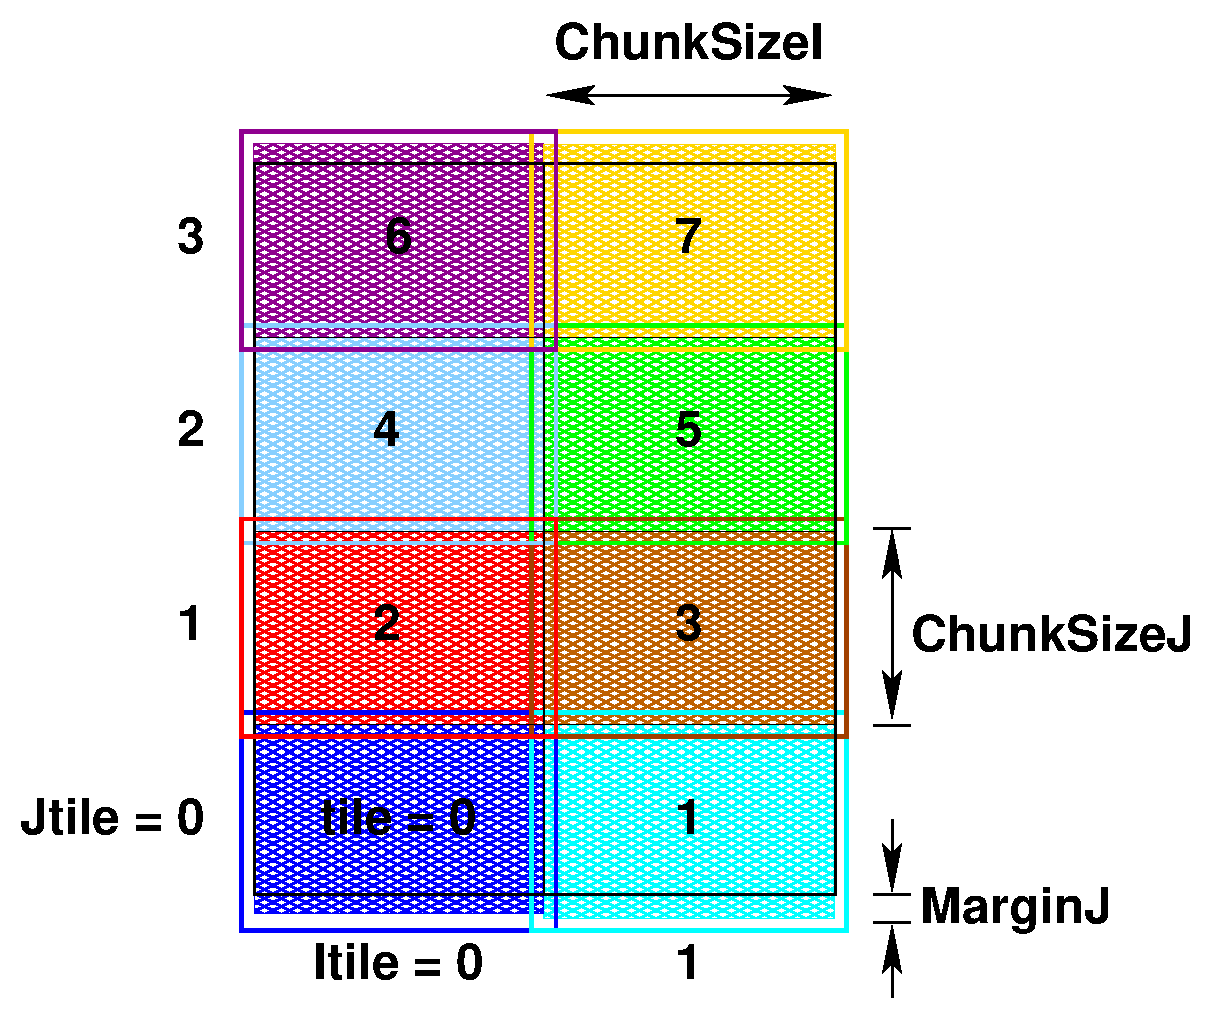
\includegraphics[height=100mm]{pics/tile3}
  \end{picture}
  \caption{A tiled grid with some ROMS tile variables.}
  \label{ftile2}
\end{figure}

The number of tiles is set in the input file as \code{NtileI}
and \code{NtileJ}. For an MPI job, the product of the two must
equal the number of MPI processes. For an OpenMP job, the
number of tiles must be a multiple of the number of threads.
For instance, for \code{NtileI}$=4$ and \code{NtileJ}$=6$, you
must have 24 MPI processes while 2, 3, 4, 6, 8, 12 and 24 are all valid
numbers of OpenMP threads. Also, a serial run could have 24
tiles and would just compute them sequentially.

Once the input file
has been read, we can compute the tile sizes in \code{get\_bounds}:
\begin{verbatim}
     ChunkSizeI = (Lm+NtileI-1)/NtileI
     ChunkSizeJ = (Mm+NtileJ-1)/NtileJ
     MarginI = (NtileI*ChunkSizeI-Lm)/2
     MarginJ = (NtileJ*ChunkSizeJ-Mm)/2
\end{verbatim}
Some internal ROMS numbers are shown in Fig.\ \ref{ftile2} and
are in the \code{BOUNDS} structure in \code{mod\_param.F}.
\code{MarginI} and \code{MarginJ} are zero if the numbers work
out perfectly, i.e.\ \code{Lm}/\code{NtileI} and
\code{Mm}/\code{NtileJ} are integers. The tile numbers match
the MPI process numbers.

In picking a numbering scheme for indices within a tile, there
are two common choices, as shown in Fig.\ \ref{fdecomp1}. Each
tile can be numbered from 1 to \code{ChunksizeI} or it can retain the
numbering it would have in the whole grid. We have chosen this
second option for ease when debugging features such as river
inputs which apply to specific locations on the grid. It is
simple to do using Fortran 90 dynamic memory allocation.

\begin{figure}[t]
\setlength{\unitlength}{10mm}
\begin{picture}(0,7)(0,0)
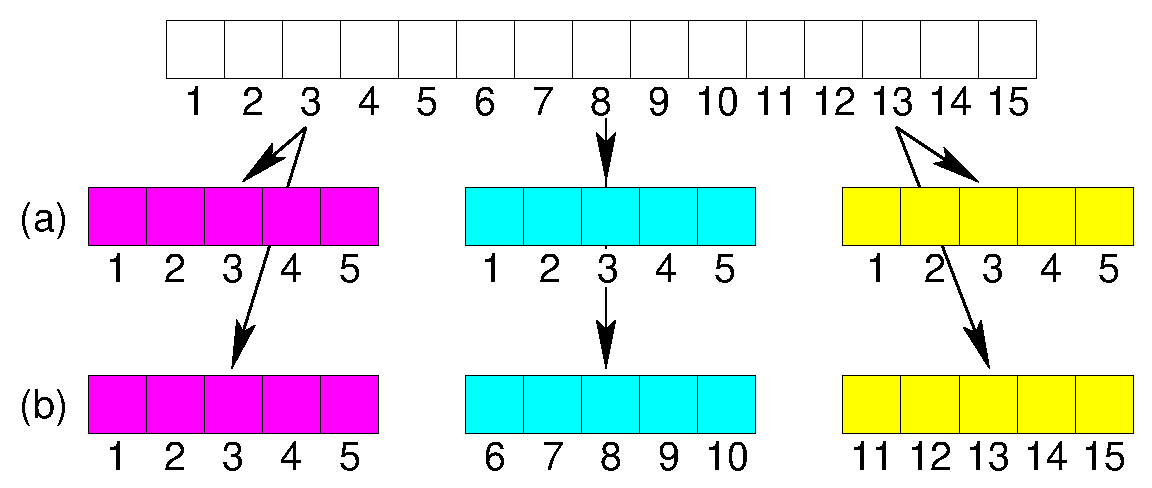
\includegraphics[width=165mm]{pics/numbering}
  \end{picture}
  \caption{A choice of numbering schemes: (a) each tile is numbered
the same, and (b) each tile retains the numbering of the parent
domain.}
  \label{fdecomp1}
\end{figure}

With the tile sizes known, we can assign beginning and ending
indices for each tile. Some of the details depend on whether or
not the domain is periodic in that direction, as shown in Fig.\
\ref{ftile3}.

\begin{figure}[tb]
\setlength{\unitlength}{10mm}
\begin{picture}(0,9)(0,0)
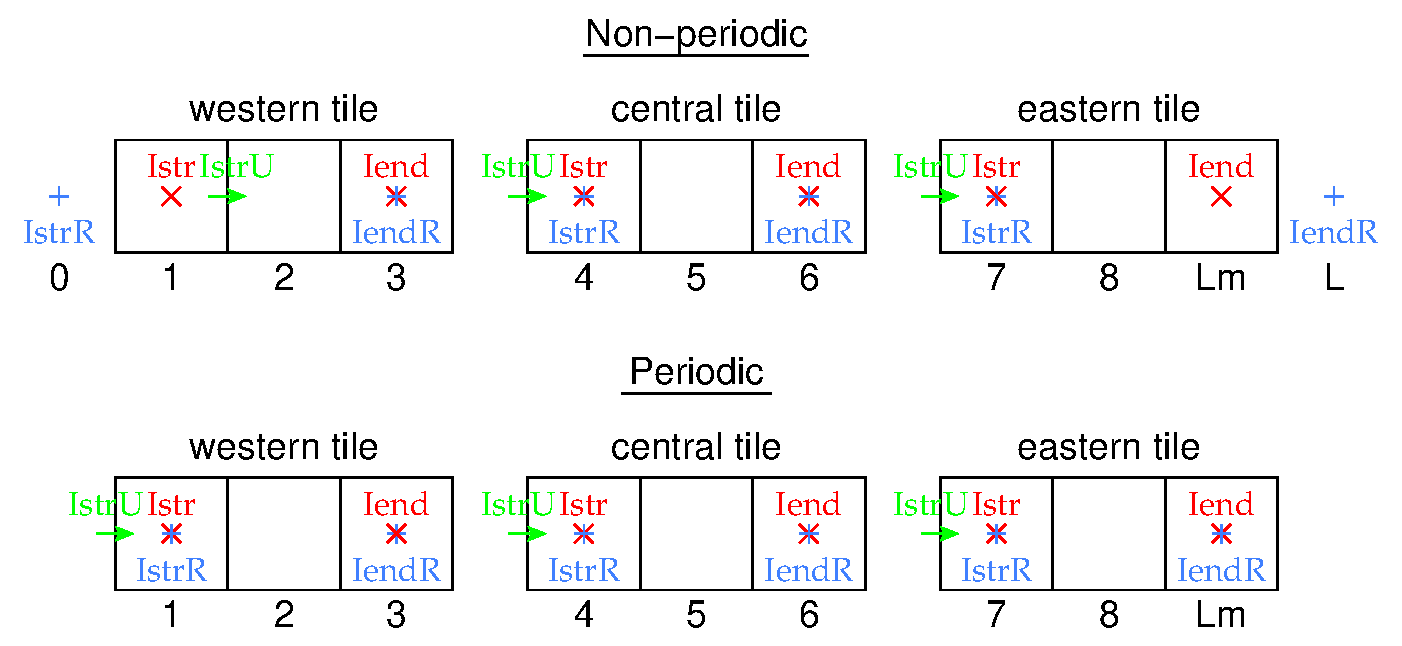
\includegraphics[width=165mm]{pics/Istr}
  \end{picture}
  \caption{Some ROMS variables for tiles, for both a periodic and
  non-periodic case. Shown are the variables in the
  \code{i}-direction, the \code{j}-direction is similar.}
  \label{ftile3}
\end{figure}

\subsubsection{MPI exchange}

For MPI jobs, the ghost points need to be updated between
interior point computations. The routines
\code{mp\_exchange2d}, \code{mp\_exchange3d} and
\code{mp\_exchange4d} can be used to update the halo points of
up to four arrays at a time. Each of these routines calls
\code{tile\_neighbors} to figure out which tiles are neighboring and
whether or not there really is a neighboring tile on each side. The
\code{mp\_exchangexd} routines then call:
\begin{verbatim}
    mpi_irecv
    mpi_send
    mpi_wait
\end{verbatim}
The exchanges happen first in the east-west direction, then in the
north-south direction, saving the need for diagonal exchanges. A figure
with interior points colored by tile and grey halo points needing an
update is shown in Fig.\ \ref{fex_2d1}(a). The updated halo points are
shown in Fig.\ \ref{fex_2d1}(b).

\begin{figure}[p]
\setlength{\unitlength}{10mm}
\begin{picture}(0,22)(-2.8,0)
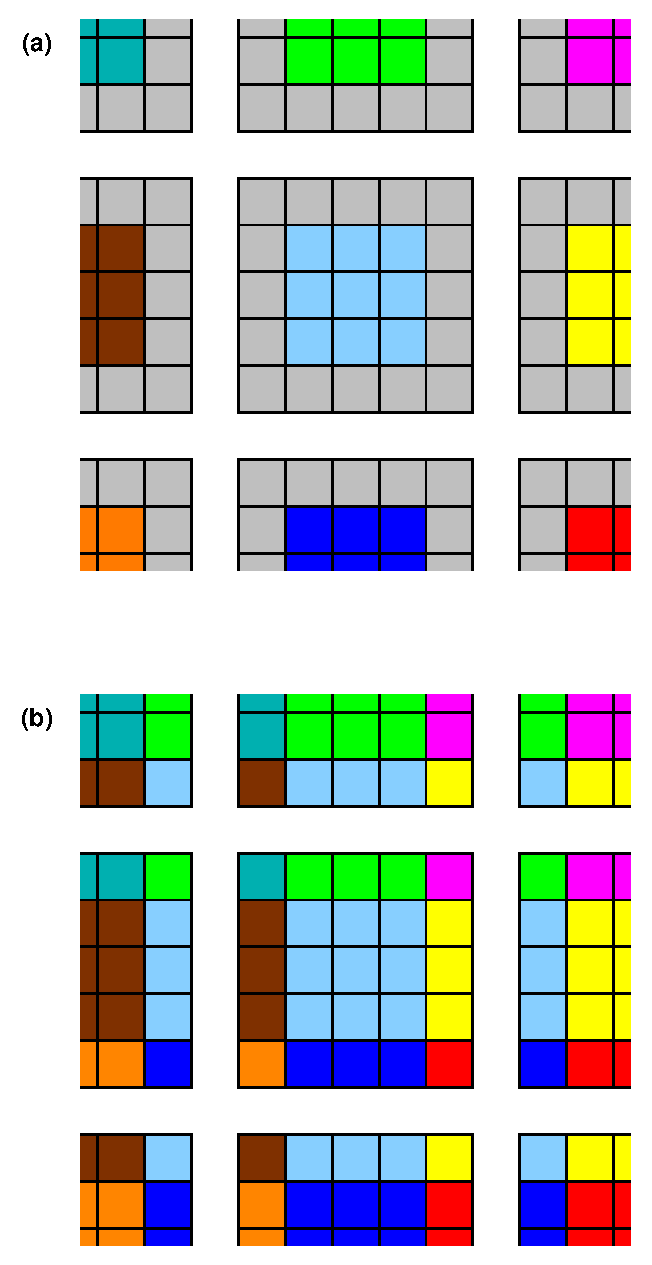
\includegraphics[height=220mm]{pics/ex_2d}
  \end{picture}
  \caption{A tiled grid with out-of-date halo regions shown in
  grey and the interior points color-coded by tile: (a) before an
  exchange and (b) after an exchange.} \label{fex_2d1}
\end{figure}

\subsubsection{Code syntax}

In \code{main3d}, many function calls are surrounded by
nesting code such as:
\begin{verbatim}
            DO ig=1,GridsInLayer(nl)
              ng=GridNumber(ig,nl)
              DO tile=first_tile(ng),last_tile(ng),+1
                CALL set_data (ng, tile)
              END DO
!$OMP BARRIER
            END DO
            IF (exit_flag.ne.NoError) RETURN
\end{verbatim}
where \code{first\_tile} and \code{last\_tile} are set in
\code{nl\_ocean.h}:
\begin{verbatim}
#if defined _OPENMP
      MyThread=my_threadnum()
#elif defined DISTRIBUTE
      MyThread=MyRank
#else
      MyThread=0
#endif
      DO ng=1,Ngrids
        chunk_size=(NtileX(ng)*NtileE(ng)+numthreads-1)/numthreads
        first_tile(ng)=MyThread*chunk_size
        last_tile (ng)=first_tile(ng)+chunk_size-1
      END DO
\end{verbatim}
\code{NtileX} and \code{NtileE} no longer depend on whether we're
using MPI:
\begin{verbatim}
      NtileX(1:Ngrids)=NtileI(1:Ngrids)
      NtileE(1:Ngrids)=NtileJ(1:Ngrids)
\end{verbatim}
Instead, \code{numthreads} varies, being set to 1 for serial jobs,
to the number of MPI processes for MPI and to
\code{omp\_get\_max\_threads()} for OpenMP jobs. For MPI jobs,
integer division gives \code{chunk\_size} the value of 1 and
\code{first\_tile} and \code{last\_tile} are both set to the process
number.

In looking at a typical routine that's called from \code{main3d},
the routine is usually quite short, calling a \code{\_tile}
version of itself in which the actual work happens:
\begin{verbatim}
    SUBROUTINE set_data (ng, tile)
    # include "tile.h"
      CALL set_data_tile (ng, tile,                        &
     &                    LBi, UBi, LBj, UBj,              &
     &                    IminS, ImaxS, JminS, JmaxS)
      RETURN
      END SUBROUTINE set_data
\end{verbatim}
Here, there are two sets of array lower and upper bounds, those
in the \code{LBi} family and those in the \code{IminS} family. Both
depend on the \code{Istr} family shown in Fig.\ \ref{ftile3}. The
\code{IminS} family is for work arrays that are local to an MPI
process or to an OpenMP thread, also local to a \code{\_tile}
routine. They are initialized:
\begin{verbatim}
      IminS=BOUNDS(ng)%Istr(tile)-3
      ImaxS=BOUNDS(ng)%Iend(tile)+3
      JminS=BOUNDS(ng)%Jstr(tile)-3
      JmaxS=BOUNDS(ng)%Jend(tile)+3
\end{verbatim}
and used:
\begin{verbatim}
      real(r8), dimension(IminS:ImaxS,JminS:JmaxS) ::  work1
      real(r8), dimension(IminS:ImaxS,JminS:JmaxS) ::  work2
\end{verbatim}
The \code{Istr} and \code{LBi} families are dimensioned by the number
of tiles once it is known by \code{inp\_par}:
\begin{verbatim}
        DO ng=1,Ngrids
          Ntiles=NtileI(ng)*NtileJ(ng)-1
          allocate ( BOUNDS(ng) % LBi  (-1:Ntiles) )
                          :
          allocate ( BOUNDS(ng) % Jend (-1:Ntiles) )
        END DO
\end{verbatim}
They are then initialized in calls to the routines in
\code{get\_bounds.F}. \code{Imin} is set to \code{-NghostPoints}
or zero, for periodic and non-periodic domains, respectively. The
\code{UBi} family is set once the \code{Istr} family is known:
\begin{verbatim}
        IF ((Itile.eq.-1).or.(Itile.eq.0)) THEN 
          LBi=Imin
        ELSE
          LBi=Istr-Nghost
        END IF
\end{verbatim}

In the case of \code{set\_data}, we are simply passing array indices
for the tiled arrays. To access the tiled arrays from within
\code{set\_data\_tile}, we need to \code{use} the relevant modules
and then refer to the array with its full name:
\begin{verbatim}
      USE mod_forces
            :
      CALL set_2dfld_tile (ng, tile, iNLM, idCfra,             &
     &                     LBi, UBi, LBj, UBj,                 &
     &                     FORCES(ng)%cloudG,                  &
     &                     FORCES(ng)%cloud,                   &
     &                     update)
\end{verbatim}
In other cases, the parent routine would have the \code{use}, then
would pass the relevant array to the \code{\_tile} routine:
\begin{verbatim}
      USE mod_grid
          :
      CALL prsgrd_tile (ng, tile,                              &
          :
     &                  GRID(ng) % Hz,                         &
          :
      SUBROUTINE prsgrd_tile (ng, tile,                        &
          :
     &                        Hz, z_r, z_w,                    &
          :
      real(r8), intent(in) :: Hz(LBi:,LBj:,:)
\end{verbatim}
This allows the \code{\_tile} routine to use \code{Hz} with the same
syntax as the pre-parallel, pre-module code once had.

\subsubsection{Input/output}

In ROMS, the distributed memory I/O is all happening on the master process
(0) unless you specifically ask it to use MPI-I/O, which requires
either or both of \code{PARALLEL\_IN}, \code{PARALLEL\_OUT} and
either of the \code{HDF5} or \code{PNETCDF} \code{cpp} flags to be
defined. If you choose \code{HDF5}, you will be reading and/or writing
\code{HDF5} files and will need to update your pre- and post-processing
tools accordingly. I have tentatively tried the parallel I/O and
found it to be exceedingly slow---I've been told since that this
is the fault of the \code{NetCDF-4} layer sitting on top of
\code{HDF5}---\code{HDF5} alone should be fast.

In the case of having all the I/O pass through the master process,
we can still read and write classic NetCDF-3 files. Care must be
taken though, in the event of an error. ROMS has been cleaned up so
that the master process will broadcast its return state to the other
processes and they can all die gracefully together when there is a
problem.

An example of a routine which reads from disk is \code{get\_grid},
called from \code{initial}. Each MPI process calls \code{get\_grid}:
\begin{verbatim}
        CALL get_grid (ng, iNLM)
# ifdef DISTRIBUTE
        CALL mp_bcasti (ng, iNLM, exit_flag)
# endif
        if (exit_flag.ne.NoError) RETURN
\end{verbatim}
If any one of the processes has trouble, it will enter into the
\code{exit\_flag} which is then shared by all.

To read in an array variable, all processes in \code{get\_grid} use
\code{nf\_fread2d} and friends:
\begin{verbatim}
            status=nf_fread2d(ng, model, ncname, ncGRDid(ng),      &
     &                        var_name(it), var_id(it),            &
     &                        0, gtype, Vsize,                     &
     &                        LBi, UBi, LBj, UBj,                  &
     &                        Fscl, Fmin, Fmax,                    &
     &                        GRID(ng) % rmask,                    &
     &                        GRID(ng) % rmask)
            IF (status.ne.nf90_noerr) THEN
              exit_flag=2
              ioerror=status
              EXIT
            END IF
\end{verbatim}
Within \code{nf\_fread2d}, we get to a call to the NetCDF library
from just the master process:
\begin{verbatim}
      IF (InpThread) THEN
        status=nf90_get_var(ncid, ncvarid, wrk, start, total)
            :
      END IF
# ifdef DISTRIBUTE
      CALL mp_bcasti (ng, model, status)
# endif
      IF (status.ne.nf90_noerr) THEN
        exit_flag=2
        ioerror=status
        nf_fread2d=status
        RETURN
      END IF
\end{verbatim}
At this point, the master process has the entire 2-D array stored in
\code{wrk}. This then needs to be divvied out to the various tiles
to their copy of the array in question (stored in the \code{A}
argument to \code{nf\_fread2d}):
\begin{verbatim}
    # ifdef DISTRIBUTE
            CALL mp_scatter2d (ng, model, LBi, UBi, LBj, UBj,         &
         &                     Nghost, MyType, Amin, Amax,            &
    #  if defined READ_WATER && defined MASKING
         &                     NWpts, SCALARS(ng)%IJwater(:,wtype),   &
    #  endif
         &                     Npts, wrk, A)
\end{verbatim}
Something similar happens when writing to output files.

\paragraph{PIO}
I have a branch in which I linked to the
\href{https://github.com/NCAR/ParallelIO}{Parallel-IO} or PIO library
from NCAR. It's unstable for fewer writers than processes, but let
me know if you'd like to try it.

%\section{Configuring ROMS for a Specific Application}
\label{Wave}
This chapter describes the parts of ROMS for which the user is
responsible when configuring it for a given application.  Section
\ref{User} describes the process in a generic fashion while
\S\ref{UpDown} and \S\ref{ARCTIC} step through the application of ROMS
to upwelling/downwelling and wind-driven Arctic problems,
respectively.  As distributed, ROMS is ready to run quite a few
examples, where the C preprocessor flags determine which is to be
executed.  Some of these examples are described in
\citet{Haidvogel99}, some are listed here:
\begin{klist}
   \kitem{BASIN} This is a rectangular, flat-bottomed basin with
 double-gyre wind forcing. When run, it produces a western boundary
 current flowing into a central ``Gulf Stream''
 which goes unstable and generates eddies. The goal is to run
 adiabatically to study the homogenization of potential vorticity.
 It earned its nickname of Big Bad Basin by taking a long time to
 run and causing difficulties for the spectral versions of SPEM.
%   \kitem{CANYON\_A} The canyon is a periodic channel with a steep shelf
% along one wall, where the shelf contains a steep canyon.  There is a
% periodic forcing which causes the water to oscillate along the
% channel.  The rotation and the shelf lead to non-zero mean flows,
% especially near the canyon.  Version A is homogeneous and can be
% executed with a 2-D model.  See \citet{HB97} for
% a description of the canyon problems and the gravitational adjustment
% problem.
%   \kitem{CANYON\_B} This is like Canyon A, except that it is
% stratified.
%   \kitem{DAMEE\_4}  DAMEE stands for Data Assimilation and Model
% Evaluation Experiment and is a comparison of different models of
% the North Atlantic.  Version 4 is a big domain
% extending from 30$^\circ$ S to 65$^\circ$ N.  Additional input files
% are required to run the DAMEE configurations.
   \kitem{GRAV\_ADJ} The gravitational adjustment problem takes place
 in a long narrow domain which is initialized with dense water at one
 end and light water at the other. At time zero, the water is released
 and it generates two propagating fronts as the light water rushes to
 fill the top and the dense water rushes to fill the bottom. This
 configuration can be used to test various advection schemes.
   \kitem{OVERFLOW}   This configuration is similar to the
 GRAV\_ADJ problem, but is initialized with dense water in the shallow
part of a domain with a sloping bottom.
   \kitem{SEAMOUNT}   The seamount test has been used to test the pressure
 gradient errors.  It has an idealized seamount in a periodic channel.
 See \citet{BH93} and \citet{McCalpin94} for more information.
   \kitem{UPWELLING}  The upwelling/downwelling example was
 contributed by \citet{Macks93}
 and consists of a periodic channel with shelves on each side.
 There is along-channel wind forcing and the Coriolis term leads
 to upwelling on one side and downwelling on the other side. If
 you run it for several days without vertical mixing, you end up with
 dense water over light water.
\end{klist}
Some NetCDF input files for the ROMS examples can be found under
\code{Data/ROMS} in the ROMS distribution. The ASCII input files are
under \code{ROMS/External}.

\subsection{Configuring ROMS}
\label{User}

The four main sections you need to change in ROMS are the \code{makefile}
or \code{build.bash}, an include file with \code{cpp} options, any
analytic functions, and the ASCII input file. If more realistic fields
are desired, you will have to provide other input files as well, for
instance for the grid and the wind forcing.

\subsubsection{Case Name}

First, you need to decide on a name for your particular application or
configuration. This name is provided via the \code{ROMS\_APPLICATION} in
either the makefile or the build script. This name should be reasonably
short, all uppercase, with spaces converted to underscores. For example,
let's say we pick the name \code{WIKI\_TEST}. This name gets defined
during the build, so you can add code protected by \code{\#ifdef
WIKI\_TEST} as needed. This would be a good time to either copy the
makefile or the build Script to create one specific to this case prior
to editing it.

\subsubsection{ Case-specific Include File}

Each application has its own include file, included by
\code{cppdefs.h}. The name of this file is the name of your
application (\code{WIKI\_TEST} here) turned into lower case, with '.h'
appended (\code{wiki\_test.h}). The location of this file is set by
\code{MY\_HEADER\_DIR}, pointing to \code{User/Include} or some other
location of your choosing.

The complete list of options to be set prior to compilation are listed in
\S\ref{Cpp1}. Place those you need in the \code{wiki\_test.h} file. These
include algorithm choices (e.g. advection and turbulence closure schemes),
output options (averages, diagnostics, stations, floats), and
application modules (biology, sediments). Each line should be of the
form:
\begin{verbatim}
        #define SOME_VAR
\end{verbatim}
Note that any undefined variable need not be mentioned.

Also note that if you copy a predefined application from
\code{ROMS/Include} as a template for your application, you must
rename it. If you don't change the name, ROMS will use the one in
\code{ROMS/Include} and your file will be ignored during the build
procedure.

\subsubsection{Functionals}

Some of the cpp options have names beginning with \code{ANA\_}. For each one of
these, you will be expected to provide an analytic expression for the field
in question in the corresponding include file. These files
are listed in \S\ref{Functionals} and their location is determined
by \code{MY\_ANALYTICAL\_DIR}. You may chose to copy those from
\code{User/Functionals} to some new directory and place your version of
the assignments within
\begin{verbatim}
        #ifdef WIKI_TEST
        ! Set weird and wonderful winds
           :
        #endif
\end{verbatim}
This makes
it easy to search for later, if nothing else.

\subsubsection{\code{checkdefs.F}}

For each new \code{cpp} variable other than your application name,
it is recommended that you also
add the appropriate code to \code{checkdefs.F}, such as:
\begin{verbatim}
       #ifdef SLEET
             IF (Master) WRITE(stdout,20) 'SLEET',                      &
            &   'Sleet falling on the ice option.'
             is=lenstr(Coptions)+1
             Coptions(is:is+7)=' SLEET,'
       #endif /* SLEET */
\end{verbatim}
Note that the number ``7'' on the \code{Coptions} line must be set
according to the length of the string you are adding.  In this case 7
is for `` SLEET,'', including the comma and the space. Again, you do not
need to do this for your application name (\code{WIKI\_TEST} here),
since \code{checkdefs} will print whatever is in \code{MyAppCPP}.

\subsubsection{Model domain}
\label{Muddy}
It is assumed in this manual that \code{Ngrids} will be set to 1.
Having multiple grids talk to each other is brand new in ROMS 3.7,
with documentation appearing on the ROMS wiki (and not currently
supported in the ice model).

One of the first things the user must decide is how many grid points
to use, and can be afforded.  There are three parameters in
\code{ocean.in} which specify the grid size and one parameter for the
number of active tracers:
\begin{tabbing}
  Gnu \= Allolo \= \kill
  \> \code{Lm} \> Number of finite-difference points in $\xi$. \\
  \> \code{Mm} \> Number of finite-difference points in $\eta$. \\
  \> \code{N} \> Number of finite-difference points in the vertical. \\
  \> \code{NAT} \> Number of active tracers. \\
\end{tabbing}
The number of biological tracers is set in the \code{biology.in} file.
There are no constraints on these except $\code{Lm} \geq 2$, $\code{Mm}
\geq 2$, $\code{N} \geq 2$ and $\code{NAT} \geq 1$.  \code{Lm} and
\code{Mm} should be at least 3 if the domain is periodic in that
direction.

\subsubsection{$x,y$ grid}
The subroutine \code{get\_grid} or \code{ana\_grid} is called by
\code{initial} to set the grid arrays, the bathymetry, and the
Coriolis parameter.  Most of the simple test problems have their grid
information specified in \code{ana\_grid.h} in the directory
\code{ROMS/Functionals}.  More realistic problems require a NetCDF grid
file, produced by the grid generation programs described in
\citet{GRIDS}, by the Matlab \code{SeaGrid}, or by some
other method.  The variables which are read by \code{get\_grid} are:
\begin{tabbing}
  Gnu \= \kill
  \> \code{xl, el, spherical, f, h, pm, pn, x\_rho, y\_rho,
  lon\_rho, lat\_rho, angle}.
\end{tabbing}
If the grid is curved, \code{get\_grid} will also read:
\begin{tabbing}
  Gnu \= \kill
  \> \code{dndx, dmde}.
\end{tabbing}
Likewise, if \code{MASKING} is defined, it will read:
\begin{tabbing}
  Gnu \= \kill
  \> \code{mask\_rho, mask\_u, mask\_v, mask\_psi}.
\end{tabbing}

\subsubsection {$\xi,\eta$ grid}
Before providing initial conditions and boundary conditions, the
user must understand the model grid. The fields are laid out on an
Arakawa C grid as in Fig.\ \ref{fcgr}. The overall grid is shown in
Fig.\ \ref{fwgr}.  The thick outer line shows the position of the
model boundary. The points inside this boundary are those which are
advanced in time using the model physics. The points on the boundary
and those on the outside must be supplied by the boundary
conditions.

The three-dimensional model fields are carried in four-dimensional
arrays, where the fourth array index refers to one of two or three
time levels. The tracers have a fifth array index telling which
tracer is being referred to.
For instance, $\code{itemp}=1$ refers to
potential temperature while $\code{isalt}=2$ refers to salinity.  The
integers $i$, $j$, and $k$ are used throughout the model to index
the three spatial dimensions:
\begin{tabbing}
Gnus \= Gnus \= \kill
   \>$i$ \>Index variable for the $\xi$-direction. \\
   \>$j$ \>Index variable for the $\eta$-direction. \\
   \>$k$ \>Index variable for the $\sigma$-direction.  $k = 1$
   refers to the bottom \\
biggnu \= \kill
   \>while $k = \code{N}$ refers to the surface.
\end{tabbing}

%The range of $\xi$ is 1 to \code{L} and the range of $\eta$ is 1 to
%\code{M}.  Therefore $i$ and $\xi$ are the same at $\psi$
%points, as are $j$ and $\eta$.  (This matters in the floats---Dale and
%I disagreed on how this should be and then Dale later changed to my
%point of view after I had recoded things to match his).

\subsubsection{Initial conditions}
The initial values for the model fields are provided by either
\code{ana\_initial} or \code{get\_state}.  \code{get\_state} is
also used to read a restart file if the model is being restarted from a
previous run.

Also in \code{initial}, \code{rho\_eos} is called to initialize
the density field. \code{rho\_eos} also computes \code{rhoA},
the vertically averaged density, and \code{rhoS}, the density
perturbation. Both \code{rhoA} and \code{rhoS} are used in the barotropic
pressure gradient.

%The tracer climatology fields also require appropriate values if they
%are to be used, and are provided by \code{ana\_tclima} or
%\code{get\_tclima}. Likewise, the surface height climatology is read by
%\code{get\_ssh} or provided by \code{ana\_ssh}.

\subsubsection{Equation of state}
The equation of state is defined in the subroutine \code{rho\_eos}.  Two
versions are provided in ROMS: a nonlinear $\rho =
\rho(T,S,z)$ from \citet{Jackett} and a linear
$\rho(T,S)$.  The linear form is
$$
      \rho = \code{R0} - \code{Tcoef} \cdot (T-T0) +
      \code{Scoef} \cdot (S-S0)
$$
or
$$
     \rho = \code{R0} + \code{Tcoef} \cdot (T-T0),
$$
depending on whether or not
\code{SALINITY} is defined.  Specify which equation of state you
would like to use with the \code{NONLIN\_EOS} C preprocessor flag in your
application include file. The linear coefficients \code{R0}, \code{T0},
\code{Tcoef}, \code{S0}, and \code{Scoef} are set in \code{ocean.in}. Note
that we are computing {\em in situ} density from potential temperature and
salinity. Some of the vertical mixing schemes require potential density
and some other fields, which are computed by \code{rho\_eos} as well.

\subsubsection{Boundary conditions}
\label{Bcs}
The horizontal boundary conditions are provided by the subroutines
in \code{u3dbc\_im}, \code{v3dbc\_im}, \code{u2dbc\_im}, \code{v2dbc\_im},
\code{t3dbc\_im}, and \code{zetabc}.  They are called every time-step
and provide the boundary values for the fields $u, v, \overline{u},
\overline{v}$, all tracers, and $\zeta$, respectively. They are currently
configured for a closed basin, a periodic channel, a doubly periodic
domain or a domain with various open boundary conditions. Each side is
controlled independently with ``West'' being the \code{i=1} boundary,
``East'' being the \code{i=L} boundary, ``South'' being the \code{j=1}
boundary, and ``North'' being the \code{j=M} boundary. These choices are
set in \code{ocean.in} via the \code{LBC} array.

Many of the choices for open boundaries require that the model have
some boundary values for the field in question. These can be specified in
the appropriate \code{ana\_xxx.h} file for say \code{ANA\_TOBC} or
they can be read from a boundary NetCDF file. There is logic in
\code{globaldefs.h} by which ROMS decides whether or not it needs to
read a boundary file.

\subsubsection{Model forcing}
\label{Mforce}
\noindent {\bf(a) Winds and thermal fluxes}

There are two different ways to apply a wind forcing: as a surface
momentum flux in the vertical viscosity term, or as a body force over
the upper water column.
Usually, we set the vertical $\sigma$-coordinate
parameters to retain some resolution near the surface and apply the
fluxes as boundary conditions to the vertical viscosity/diffusivity.
In either case, the surface and bottom fluxes are either defined
analytically, read from a forcing file, or computed inside ROMS
using a bulk flux formula from the appropriate atmospheric fields
(air temperature and winds, for instance).  You must either edit the
appropriate \code{ana\_xxx.h} or create a NetCDF forcing
file in the format expected by ROMS. Note that it is quite common
to put the surface variables in the forcing file while having an analytic
bottom heat flux. ROMS now has the capability of reading in a list
of forcing fields---it can be convenient to have one file per field
rather than stuffing tides, winds, river inputs all into one file.

In the past, our vertical resolution was relatively coarse and the
vertical viscosity would have to have been unreasonably large for
us to resolve the surface Ekman layer.  If that is your situation,
define \code{BODYFORCE} in \code{cppdefs.h} and provide a value for
\code{levsfrc} in \code{ocean.in}.  The forcing is applied over the
levels from \code{levsfrc} to \code{N}.  The above caution about
vertical resolution also applies to the surface fluxes of $T$ and
$S$, although \code{BODYFORCE} only refers to wind stress, not the
surface tracer fluxes.

\smallskip
\noindent {\bf(b) Climatology}

One way to force the model is via a nudging to the tracer and/or
momentum climatologies. Nudging to tracers was used in the North
Atlantic simulations in sponge layers along the northern and southern
boundaries. Set the climatologies in \code{ana\_tclima.h} or in a
file read by \code{get\_data}, set \code{TCLM\_NUDGING} in
\code{wiki\_test.h} and also set the array \code{Tnudgcof} in
\code{ana\_nudgcoef.h}.

\smallskip
\noindent {\bf(c) Tides}

There is also more than one way to force with tides. One way is to
provide boundary conditions with enough temporal resolution to
resolve the tides. Another is to provide ROMS with the tidal
constituents at all grid points and to have ROMS reconstruct the
tidal currents (\code{UV\_TIDES})  and/or elevations (\code{SSH\_TIDES})
for any given time. An example of such a tidal forcing file is in
\code{Data/ROMS/Forcing/test\_head\_frc.nc}.

The non-trunk code with ice, etc. includes the \code{TIDES\_ASTRO} option to
add on the long-period tides from
\citet{Foreman_96a} and \citet{Foreman_96b}.
There is also an option to include the tidal potential
forcing term (\code{POT\_TIDES}), requiring the tidal potential to
be included in the tides forcing file.

\smallskip
\noindent {\bf(d) Rivers}

Point sources can be used to provide river inflow to the model.
These too can be specified in a forcing file if not provided via
\code{ana\_psource}.

\subsubsection{\code{ocean.in}}
\label{ASCII_in}
ROMS expects to read a number of variables from an ASCII file as described
in \S\ref{Running}.
Example input files are in \code{ROMS/External} with names like
\code{ocean\_grav\_adj.in}, where ``grav\_adj'' refers to the name of
the application. Lines beginning with ``!'' are comments and will be
ignored by ROMS on reading them.

The input is organized as key/value pairs, separated by one or two
equals signs. It is possible for ROMS to run on more than one grid
simultaneously, with the number of grids being read from the input
file. If there is one equals sign (\code{=}), ROMS will use the
corresponding value for all grids. If there are two (\code{==}), ROMS
will read a value for each grid. Thus far, our domains have used just
one grid since the inter-grid coupling has only been released very
recently.

ROMS will ignore the parameters not needed by the current
simulation, e.g., the GLS parameters will not be read if you are not
using that mixing scheme. However, I believe all the example files
contain all possible parameters (except the ice branch ones).
The input parameters are in groups, as follows:
\begin{klist}
   \kitem{Header} \mbox{}
     \begin{klist}
   \kitem{TITLE} A text string to put in the output files.
   \kitem{MyAppCPP} The shorthand name for this application.
   \kitem{VARNAME} The location of the \code{varinfo.dat} file
     containing information about fields to read/write from/to NetCDF
     files.
   \kitem{Ngrids} The number of grids to compute on---usually 1 so
   far.
     \end{klist}
   \kitem{Grid-dimension parameters} \mbox{}
     \begin{klist}
       \kitem{Lm} Number of $i$-direction INTERIOR RHO-points.
       \kitem{Mm} Number of $j$-direction INTERIOR RHO-points.
       \kitem{N} Number of vertical levels.
       \kitem{Nbed} Number of sediment bed layers.
       \kitem{NAT} Number of active tracers (usually 2).
       \kitem{NPT} Number of passive tracers.
       \kitem{NCS} Number of cohesive (mud) sediment tracers.
       \kitem{NNS} Number of non-cohesive (sand) sediment tracers.
     \end{klist}
   \kitem{Domain-decomposition parameters} \mbox{}
     \begin{klist}
       \kitem{NtileI} Number of $i$-direction partitions.
       \kitem{NtileJ} Number of $j$-direction partitions.
     \end{klist}
   \kitem{Boundary conditions} \mbox{}
     \begin{klist}
       \kitem{LBC} A line is given for each field, each line
       containing four values, one for each side in the order
       ``West'', ``South'', ``East'', ``North''. Each value is a
       string, with the possible values being:
         \begin{klist}
           \kitem{Cha}   Chapman.
           \kitem{Cla}   Clamped.
           \kitem{Clo}   Closed.
           \kitem{Fla}   Flather.
           \kitem{Gra}   Gradient.
           \kitem{Nes}   Nested.
           \kitem{Nud}   Nudging.
           \kitem{Per}   Periodic---should match the opposing
boundary.
           \kitem{Rad}   Radiation.
           \kitem{RadNud}Radiation and nudging.
           \kitem{Red}   Reduced Physics---note that this also
requires the \code{FSOBC\_REDUCED} cpp flag.
         \end{klist}
       \kitem{VolCons} Four values for the volume conservation, one
for each edge.
     \end{klist}
   \kitem{Time-stepping parameters} \mbox{}
     \begin{klist}
       \kitem{NTIMES}    Number of time-steps to evolve the 3-D
       equations in the current run.  This is actually the total
     number, including any previous segments of the same run.  For
     instance, if you already did a three-month run and wish to
     continue for another three months, set \code{NTIMES} to the
     number of steps needed for six months.
       \kitem{DT}        Time-step in seconds for the 3-D equations.
       \kitem{NDTFAST}   Number of time-steps for the 2-D equations
     to be executed each \code{dt}.
     \end{klist}
   \kitem{Model iteration loops parameters} \mbox{}
     \begin{klist}
       \kitem{ERstr} Starting ensemble run number.
       \kitem{ERend} Ending ensemble run number.
       \kitem{Nouter} Maximum number of 4DVAR outer loop iterations.
       \kitem{Ninner} Maximum number of 4DVAR inner loop iterations.
       \kitem{Nintervals} Number of time interval divisions for
       stochastic optimals computations.
     \end{klist}
   \kitem{Generalized Stability Theory (GST) parameters} \mbox{}
     \begin{klist}
       \kitem{NEV} Number of eigenvalues.
       \kitem{NCV} Number of eigenvectors.
     \end{klist}
   \kitem{Input/Output parameters} \mbox{}

   ROMS has several possible output files. The output files can
   include a restart file, a history file, an averages file, and a
   station file, for instance.  The restart file often contains
   only two records with the older record being overwritten during
   the next write.  The history file can contain a subset of the
   restart fields, for instance just the surface elevation and the
   surface temperature.  The averages file contains time-averages
   of the model fields, for instance daily or monthly means,
   depending on \code{NAVG}.  The station file contains timeseries
   for specified points, possibly quite frequently since each record
   is small. For some, machinery is in place to write multiple
   files, numbering them \_0001, \_0002, etc.
     \begin{klist}
       \kitem{NRREC}     Record number of the restart file to read
     as the initial conditions. Set to 0 at the beginning of the
     run, -1 to read the latest record.
       \kitem{LcycleRST} Logical, true to cycle between two records
     of the restart file.
       \kitem{NRST}      Number of time-steps between writing of
     restart fields.
       \kitem{NSTA}      Number of time-steps between writing fields
     into the stations file.
       \kitem{NFLT}      Number of time-steps between writing fields
     into the floats file.
       \kitem{NINFO}     Number of time-steps between calling
       \code{diag} to write some global information and check for
       NaN values. 
     \end{klist}
   \kitem{History, average, diagnostic output parameters} \mbox{}
     \begin{klist}
       \kitem{LDEFOUT} True for creating new output files for
       stations, history, floats, etc. If false, output is appended
       to these files.
       \kitem{NHIS}  Number of time-steps between writing history
       records.
       \kitem{NDEFHIS}  Number of time-steps between starting new history
       files.
       \kitem{NTSAVG}    Starting time-step for the accumulation of
     output time-averaged data.  For instance, you might want to average
     over the last day of a thirty-day run.
       \kitem{NAVG}      Number of time-steps between writing
     time-averaged data into the averages file.
       \kitem{NDEFAVG}      Number of time-steps between starting
     new averages files.
       \kitem{NTSDIA}    Starting time-step for the accumulation of
     output diagnostics data.  For instance, you might want to write
     diagnostics for the last day of a thirty-day run.
       \kitem{NDIA}      Number of time-steps between writing
     diagnostics data into the diagnostics file.
       \kitem{NDEFDIA}      Number of time-steps between starting
     new diagnostics files.
     \end{klist}
    \kitem{Tangent linear and adjoint output parameters} \mbox{}
     \begin{klist}
       \kitem{LcycleTLM} Logical, true to cycle between two records
       \kitem{NTLM}      Number of time-steps between writing
     tangent linear data.
       \kitem{NDEFTLM}      Number of time-steps between starting
     new tangent linear files.
       \kitem{LcycleADJ} Logical, true to cycle between two records
     of the restart file.
       \kitem{NADJ}      Number of time-steps between writing
     adjoint data.
       \kitem{NDEFADJ}      Number of time-steps between starting
     new adjoint files.
       \kitem{NSFF}     Number of time-steps between 4DVAR adjustment of
       surface forcing fluxes.
       \kitem{NOBC}    Number of time-steps between 4DVAR adjustment of
       open boundary fields.
     \end{klist}
    \kitem{Check-pointing GST restart parameters} \mbox{}
     \begin{klist}
       \kitem{LrstGST} GST restart switch.
       \kitem{MaxIterGST} Maximum number of iterations.
       \kitem{NGST} Check-pointing interval.
     \end{klist}
    \kitem{Ritz GST parameter} \mbox{}
     \begin{klist}
       \kitem{Ritz\_tol} Relative accuracy of the Ritz values
       computed in the GST analysis.
     \end{klist}
   \kitem{Horizontal mixing of tracers} \mbox{}
     \begin{klist}
       \kitem{TNU2}     Constant mixing
     coefficient for the horizontal Laplacian diffusion of each tracer.
     A value is expected for each of the \code{NAT+NPT} tracers.
       \kitem{TNU4}     Constant mixing
     coefficient for the horizontal biharmonic diffusion of each tracer.
     A value is expected for each of the \code{NAT+NPT} tracers.
     \end{klist}
   \kitem{Horizontal viscosity coefficients} \mbox{}
     \begin{klist}
       \kitem{VISC2}    Constant mixing coefficient for the horizontal
     Laplacian viscosity.
       \kitem{VISC4}    Constant mixing coefficient for the horizontal
     biharmonic viscosity.
     \end{klist}
   \kitem{Vertical mixing coefficients for tracers} \mbox{}
     \begin{klist}
       \kitem{AKT\_BAK}  Background vertical mixing coefficient
     for the tracers (\code{NAT+NPT} values).
     \end{klist}
   \kitem{Vertical mixing coefficient for momentum} \mbox{}
     \begin{klist}
       \kitem{AKV\_BAK}  Background vertical mixing coefficient 
     for momentum.
     \end{klist}
   \kitem{Turbulent closure parameters} \mbox{}
     \begin{klist}
       \kitem{AKK\_BAK}  Background vertical mixing coefficient
     for turbulent kinetic energy.
       \kitem{AKP\_BAK}  Background vertical mixing coefficient
     for turbulent generic statistical field.
       \kitem{TKENU2}    Constant mixing coefficient for the horizontal
     Laplacian diffusion of turbulent kinetic energy.
       \kitem{TKENU4}    Constant mixing coefficient for the horizontal
     biharmonic diffusion of turbulent kinetic energy.
     \end{klist}
   \kitem{Generic length-scale turbulence closure parameters}
   \mbox{}
     \begin{klist}
       \kitem{GLS\_P}   Stability exponent.
       \kitem{GLS\_M}   Turbulent kinetic energy exponent.
       \kitem{GLS\_N}   Turbulent length scale exponent.
       \kitem{GLS\_Kmin}  Minimum value of specific turbulent kinetic
       energy.
       \kitem{GLS\_Pmin}  Minimum value of dissipation.
       \kitem{GLS\_CMU0}   Stability coefficient.
       \kitem{GLS\_C1}   Shear production coefficient.
       \kitem{GLS\_C2}   Dissipation coefficient.
       \kitem{GLS\_C3M}   Buoyancy production coefficient (minus).
       \kitem{GLS\_C3P}   Buoyancy production coefficient (plus).
       \kitem{GLS\_SIGK} Constant Schmidt number (non-dimensional) for
       turbulent kinetic energy diffusivity.
       \kitem{GLS\_SIGP}  Constant Schmidt number (non-dimensional) for
       turbulent generic statistical field, ``psi''.
     \end{klist}
   \kitem{Constants used in surface TKE flux computation} \mbox{}
     \begin{klist}
       \kitem{CHARNOK\_ALPHA} Charnok surface roughness.
       \kitem{ZOS\_HSIG\_ALPHA} Roughness from wave amplitude.
       \kitem{SZ\_ALPHA} Roughness from wave dissipation.
       \kitem{CRGBAN\_CW} Craig and Banner wave breaking.
     \end{klist}
   \kitem{Bottom drag coefficients} \mbox{}
     \begin{klist}
       \kitem{RDRG}     Linear bottom drag coefficient.
       \kitem{RDRG2}    Quadratic bottom drag coefficient.
       \kitem{Zob}       Bottom roughness.
       \kitem{Zos}       Surface roughness (under ice shelves).
     \end{klist}
   \kitem{Height of atmospheric measurements for bulk flux
   parameterizations} \mbox{}
     \begin{klist}
       \kitem{BLK\_ZQ} Height of air humidity values.
       \kitem{BLK\_ZT} Height of air temperature values.
       \kitem{BLK\_ZW} Height of wind values.
     \end{klist}
   \kitem{Wetting and drying parameter} \mbox{}
     \begin{klist}
       \kitem{DCRIT}  Minimum depth for dry cells.
     \end{klist}
   \kitem{Various parameters} \mbox{}
     \begin{klist}
       \kitem{WTYPE}  Jerlov water type.
       \kitem{LEVSFRC}  Deepest level to apply surface momentum
     stresses as a body force.
            Used when the C-preprocessor option BODYFORCE is defined.
       \kitem{LEVBFRC}  Shallowest level to apply bottom momentum
    stresses as a body force.
            Used when the C-preprocessor option BODYFORCE is defined.
     \end{klist}
   \kitem{Vertical coordinate parameters} \mbox{}
     \begin{klist}
       \kitem{Vtransform} Transformation equation, 1 for old style.
       \kitem{Vstretching} Stretching function, 1 for old style.
     \end{klist}
   \kitem{Vertical $\sigma$-coordinates parameters} \mbox{}
     \begin{klist}
       \kitem{THETA\_S}  $\sigma$-coordinate surface control parameter,
     [$0 < \code{theta\_s} < 20$].
       \kitem{THETA\_B}  $\sigma$-coordinate bottom  control parameter,
     [$0 < \code{theta\_b} < 1$].
       \kitem{TCLINE}   Width of the surface or bottom boundary layer
     in which higher vertical resolution is required during stretching.
     \end{klist}
   \kitem{Mean Density and Brunt-V\"ais\"al\"a frequency} \mbox{}
     \begin{klist}
       \kitem{RHO0}     Mean density used in the Boussinesq
     approximation.
       \kitem{BVF\_BAK} Background Brunt-V\"ais\"al\"a frequency squared.
     \end{klist}
   \kitem{Time parameters} \mbox{}
     \begin{klist}
       \kitem{DSTART}   Time stamp assigned to model initialization
     (days).
       \kitem{TIDE\_START}   Time of tidal origin relative to model
       origin.
       \kitem{TIME\_REF}  Reference time in the format yyyymmdd.dd or
       else a special value for specific calendars as documented in the
       \code{ocean.in} files.
     \end{klist}
  \kitem{Nudging time scales} \mbox{}
     \begin{klist}
       \kitem{TNUDG}    Time scale (days) of nudging towards
     tracer climatology at the interior and at the boundaries.
     A value is expected for each active tracer.
       \kitem{ZNUDG}    Time scale (days) of nudging towards
     free surface climatology at the interior and at the boundaries.
       \kitem{M2NUDG}    Time scale (days) of nudging towards
     2-D momentum climatology at the interior and at the boundaries.
       \kitem{M3NUDG}    Time scale (days) of nudging towards
     3-D momentum climatology at the interior and at the boundaries.
     \end{klist}
   \kitem{Open boundary factor} \mbox{}
     \begin{klist}
       \kitem{OBCFAC}   Ratio of inflow and outflow nudging time scales.
     \end{klist}
   \kitem{Linear equation of state parameters} \mbox{}
     \begin{klist}
       \kitem{R0}       Background density value used in
    the linear equation of state.
       \kitem{T0}       Background potential temperature constant.
       \kitem{S0}       Background salinity constant.
       \kitem{TCOEF}    Thermal expansion coefficient in the linear
    equation of state.
       \kitem{SCOEF}    Saline contraction coefficient in the linear
    equation of state.
     \end{klist}
   \kitem{Slipperiness parameter} \mbox{}
     \begin{klist}
       \kitem{GAMMA2}   Slipperiness variable, either 1.0 (free
     slip) or $-1.0$ (no slip).
     \end{klist}
   \kitem{Tracer point sources} \mbox{}
     \begin{klist}
       \kitem{LtracerSrc} Logical, one value per tracer,
whether or not point sources have tracer values.
     \end{klist}
%   \kitem{Adjoint sensitivity time parameters} \mbox{}
%     \begin{klist}
%       \kitem{DstrS} Starting day.
%       \kitem{DendS} Ending day.
%     \end{klist}
%   \kitem{Adjoint sensitivity vertical level parameters} \mbox{}
%     \begin{klist}
%       \kitem{KstrS} Starting level.
%       \kitem{KendS} Ending level.
%     \end{klist}
%   \kitem{Adjoint sensitivity logical parameters} \mbox{}
%     \begin{klist}
%       \kitem{Lstate(isFsur)} Free surface.
%       \kitem{Lstate(isUbar)} 2D $u$-momentum.
%       \kitem{Lstate(isVbar)} 2D $v$-momentum.
%       \kitem{Lstate(isUvel)} 3D $u$-momentum.
%       \kitem{Lstate(isVvel)} 3D $v$-momentum.
%       \kitem{Lstate(isTvar)} Tracers (NT values expected).
%     \end{klist}
%   \kitem{Stochastic optimals time scale} \mbox{}
%     \begin{klist}
%       \kitem{SO\_decay}  Stochastic optimals time decorrelation
%       scale (days) assumed for red noise processes.
%     \end{klist}
%   \kitem{Logicals for stochastic optimals} \mbox{}
%     \begin{klist}
%       \kitem{SOstate(isUstr)}  Surface $u$-stress.
%       \kitem{SOstate(isVstr)}  Surface $v$-stress.
%       \kitem{Lstate(isTsur)} Surface tracer flux (NT values expected).
%     \end{klist}
%   \kitem{Stochastic optimals surface standard deviations} \mbox{}
%     \begin{klist}
%       \kitem{SO\_sdev(isUstr)} Surface $u$-stress.
%       \kitem{SO\_sdev(isVstr)} Surface $v$-stress.
%       \kitem{SO\_sdev(isTsur)} Surface tracer flux (NT values
%       expected).
%     \end{klist}
   \kitem{Logical switches to activate the writing of
   history/averages fields} \mbox{}
     \begin{klist}
       \kitem{Hout} History output switches, one line per variable.
Check the \code{ocean.in} file for the names of the fields involved. The
\code{Hout} values for the ice model are now set in \code{ice.in}.
       \kitem{Aout} Averages output switches, one line per variable.
Check the \code{ocean.in} file for the names of the fields involved. The
\code{Aout} values for the ice model are now set in \code{ice.in}.
       \kitem{Aout2} Averages2 output switches, one line per variable.
Check the \code{ocean.in} file for the names of the fields involved. The
\code{Aout2} values for the ice model are now set in \code{ice.in}.
       \kitem{Dout} Diagnostics output switches, one line per term.
Check the \code{ocean.in} file for the names of the fields involved.
     \end{klist}
   \kitem{User parameters} \mbox{}
     \begin{klist}
       \kitem{NUSER}    Number of user parameters
       \kitem{USER}     Values of user parameters (NUSER values).
     \end{klist}
   \kitem{NetCDF-4/HDF5 parameters} \mbox{}
     \begin{klist}
       \kitem{NC\_SHUFFLE}    If non-zero, turn on shuffle filter.
       \kitem{NC\_DEFLATE}    If non-zero, turn on deflate filter.
       \kitem{NC\_DLEVEL}    Deflate level (0--9).
     \end{klist}
   \kitem{Input NetCDF file names} \mbox{}
     \begin{klist}
       \kitem{GRDNAME}  Grid file.
       \kitem{ININAME}  Initial conditions file.
       \kitem{ITLNAME}  Initial tangent linear file.
       \kitem{IRPNAME}  Initial representer file.
       \kitem{IADNAME}  Initial adjoint file.
       \kitem{FWDNAME}  Forward model file.
       \kitem{ADSNAME}  Adjoint sensitivity functional file.
     \end{klist}
    \kitem{Boundary, Climatology and Forcing NetCDF files} These can
each have an array of files, with one set of files per variable,
each file in a set for a different range of times. See
\code{ocean.in} for syntax. Note that the trunk code only does this
for forcing files.
     \begin{klist}
       \kitem{NCLMFILES}  Number of climatology files.
       \kitem{CLMNAME}  Climatology file.
       \kitem{NBCFILES}  Number of boundary files.
       \kitem{BRYNAME}  Boundary condition file.
       \kitem{NFFILES}  Number of forcing files.
       \kitem{FRCNAME}  Forcing files.
     \end{klist}
    \kitem{Output NetCDF file names} \mbox{}
     \begin{klist}
       \kitem{GSTNAME}  GST analysis restart file.
       \kitem{RSTNAME}  Restart file.
       \kitem{HISNAME}  History file.
       \kitem{TLMNAME}  Tangent linear file.
       \kitem{TLFNAME}  Impulse forcing file (for tangent linear model).
       \kitem{ADJNAME}  Adjoint file.
       \kitem{AVGNAME}  Averages file.
       \kitem{AVG2NAME}  Averages2 file.
       \kitem{DIANAME}  Diagnostics file.
       \kitem{STANAME}  Stations file.
       \kitem{FLTNAME}  Lagrangian floats file.
     \end{klist}
   \kitem{ASCII input file names} \mbox{}
     \begin{klist}
       \kitem{APARNAM}  Assimilation parameters.
       \kitem{SPOSNAM}  Stations positions.
       \kitem{FPOSNAM}  Initial drifter positions.
       \kitem{IPARNAM}  Ice parameters.
       \kitem{BPARNAM}  Biology parameters.
       \kitem{SPARNAM}  Sediment parameters.
       \kitem{USRNAME}  User's generic input.
     \end{klist}
\end{klist}
The bottom of the sample files contain comments describing some of these in
greater detail.

%An example input file without the trailing comments is:
%\begin{verbatim}
%\end{verbatim}

\subsubsection{User variables and subroutines}
\label{Store}
It is possible for the user to add new variables and functionality,
though it is discouraged. The design goal is to isolate the most common
features a user would change to the \code{cpp} switches
(\S\ref{Cpp1}), the \code{ana\_xx.h} files (\S\ref{Functionals}) and
the ASCII input file (\S\ref{ASCII_in}). A query on the ROMS forum
might be in order if you have something specific in mind.

If you do choose to add bits, know that the \code{makefile}
fragments called \code{Module.mk} will attempt to compile and
link into a library anything
with a \code{.F} extension in the directories already generating a
library from such files.

\subsection{Upwelling/Downwelling Example}
\label{UpDown}
The application which ROMS is configured to run as distributed
is a wind-driven
upwelling and downwelling example, described in
\citet{Macks93}.  There is a shelf on each wall of a periodic channel
and an along-channel wind forcing, which drives upwelling at one wall
and downwelling at the other.  This problem depends on the Ekman layer,
therefore a surface stress is used with vertical viscosity.  The Ekman
depth is estimated to be 9 $m$ if $A_v = 0.01 m^2 / s$, so the vertical
grid spacing must resolve this.  The maximum depth is 150 $m$ and our
choice of the vertical grid parameters leads to a surface $\Delta z$
of 4.0 $m$.

\subsubsection{\code{cppdefs.h}}
The C preprocessor variable \code{UPWELLING} is used for the
upwelling configuration of the model. The \code{makefile} will
direct \code{cppdefs.h} to include the file \code{upwelling.h}:
\begin{verbatim}
        #define UV_ADV
        #define UV_COR
        #define UV_LDRAG
        #define UV_VIS2
        #undef  MIX_GEO_UV
        #define MIX_S_UV
        #define TS_U3HADVECTION
        #define TS_C4VADVECTION
        #undef  TS_MPDATA
        #define DJ_GRADPS
        #define TS_DIF2
        #undef  TS_DIF4
        #undef  MIX_GEO_TS
        #define MIX_S_TS

        #define SALINITY
        #define SOLVE3D
        #define SPLINES
        #define AVERAGES
        #define DIAGNOSTICS_TS
        #define DIAGNOSTICS_UV

        #define ANA_GRID
        #define ANA_INITIAL
        #define ANA_SMFLUX
        #define ANA_STFLUX
        #define ANA_SSFLUX
        #define ANA_BTFLUX
        #define ANA_BSFLUX

        #if defined GLS_MIXING || defined MY25_MIXING
        # define KANTHA_CLAYSON
        # define N2S2_HORAVG
        #else
        # define ANA_VMIX
        #endif

        #if defined BIO_FENNEL  || defined ECOSIM || \
            defined NPZD_POWELL || defined NEMURO || \
            defined BIO_UMAINE
        # define ANA_BIOLOGY
        # define ANA_SPFLUX
        # define ANA_BPFLUX
        # define ANA_SRFLUX
        #endif

        #if defined NEMURO
        # define HOLLING_GRAZING
        # undef  IVLEV_EXPLICIT
        #endif

        #ifdef BIO_FENNEL
        # define CARBON
        # define DENITRIFICATION
        # define BIO_SEDIMENT
        # define DIAGNOSTICS_BIO
        #endif

        #ifdef BIO_UMAINE
        # define OXYGEN
        # undef CARBON
        #endif

        #ifdef PERFECT_RESTART
        # undef  AVERAGES
        # undef  DIAGNOSTICS_BIO
        # undef  DIAGNOSTICS_TS
        # undef  DIAGNOSTICS_UV
        # define OUT_DOUBLE
        #endif
\end{verbatim}
Here we have declared that we want a three-dimensional solution, but
no masking. There is salinity but we're using a linear equation of state.
The momentum equations have advection, Coriolis force and pressure
gradients. There is both horizontal viscosity and diffusion, but they
are along constant $\sigma$-surfaces and if you check the input file,
you find that the horizontal diffusion is set to zero.

There are ifdefs for various biology cases, none of which
have been defined. Likewise, we are using the default of
\code{ANA\_VMIX} as distributed. We are asking for many other
analytic functions too, including the grid. We are asking
for diagnostic output with the \code{DIAGNOSTICS\_TS} and
\code{DIAGNOSTICS\_UV}.

\subsubsection{Model domain}
The flow does not vary in $x$, so \code{Lm} can be almost anything.
Set the values for \code{Lm}, \code{Mm}, \code{N} and \code{NT} in
the input file:
\begin{verbatim}
          Lm == 41            ! Number of I-direction INTERIOR RHO-points
          Mm == 80            ! Number of J-direction INTERIOR RHO-points
           N == 16            ! Number of vertical levels

         NAT =  2             ! Number of active tracers (usually, 2)
\end{verbatim}
A historical note: \code{Lm} here really is 41 for 41 boxes in the
$x$-direction. It was originally set to 41 for 40 boxes, but the
periodic boundary conditions are now more efficient and no longer
need an extra box. One could just as well set it to 40 (or even 5).

\subsubsection{\code{ana\_grid}}
For this geometry one has a choice of using one of the external
grid-generation programs or of using \code{ana\_grid} to create the grid
analytically. The code in \code{ana\_grid.h} was modified to produce a
bathymetry with a shelf on both walls of the channel when \code{UPWELLING}
is defined. The fluid depth ranges from 27 $m$ on the shelves to 150 $m$
in the center of the channel.  The horizontal grid spacing is uniform
at 1 $km$ and the Coriolis parameter $f$ is set to a constant value
suitable for Sydney, Australia.

\subsubsection{Initial conditions and the equation of state}
We would like the initial conditions to be a motionless fluid with an
exponential stratification. The \code{UPWELLING} section of
\code{ana\_initial.h} is configured accordingly.

The stratification can be provided by either $T$ or $S$, or by both
$T$ and $S$.  For
simplicity we will only have an active temperature field and we will
use the linear equation of state by setting \code{NONLIN\_EOS} to
\code{\#undef}. We want the density to be 26.35 at
the bottom and 24.22 at the top with an e-folding scale of 50 meters.
The initial temperature is set to \code{T0}$ + 8\mbox{e}^{z/50}$ in
\code{ana\_initial}.  The linear equation of state parameters are set
in \code{ocean\_upwelling.in}:
\begin{verbatim}
          R0 == 1027.0d0                   ! kg/m3
          T0 == 14.0d0                     ! Celsius
          S0 == 35.0d0                     ! PSU
       TCOEF == 1.7d-4                     ! 1/Celsius
       SCOEF == 0.0d0                      ! 1/PSU
\end{verbatim}

Since density does not depend on salinity, we have a choice of how to
handle the second tracer. The salinity is set to a uniform value
of \code{S0}, though it could be left out entirely if we undefine
\code{SALINITY} and set \code{NAT} to 1.

\subsubsection{Boundary conditions}
In \code{ocean\_upwelling.in}, the variable \code{LBC} is set to be
periodic in the East-West direction, with closed walls to the North
and South. No boundary values are required.

\subsubsection{Model forcing}
In this problem we want to resolve the
surface Ekman layer and to use a surface wind stress rather than a body
force.  We want the amplitude of the wind to ramp up with time so we
modify \code{ana\_smflux.h} accordingly.
The wind will build to an amplitude of 0.1 Pascals / $\rho_o$,
or $10^{-4} m^2 s^{-2}$.

We need to edit \code{ana\_vmix.h} to make sure that the
vertical viscosity \code{Akv} is set to the value we want.  This
must be large at the surface ($10^{-2} m^2 s^{-1}$) to create a thick
Ekman layer, but has been chosen to decrease with depth.  We also need
to check that \code{ana\_sbflux}, \code{ana\_stflux}, etc.\ are
set correctly, in this case taking the default of zero rather than
explicitly setting anything for \code{UPWELLING}. However, we do set
\code{ana\_srflux} to be non-zero in case we opt to turn on one of
the biology models.

\subsubsection{ocean.in}
The model has been set up to run for five days with an internal time-step
of 300 $s$ and an external time-step of 10 $s$.
\begin{verbatim}
      NTIMES == 1440
          DT == 300.0d0
     NDTFAST == 30
\end{verbatim}
  We will write history, averages, and diagnostics
records every 1/4 day, restart records once a day.
\begin{verbatim}
       NRREC == 0
   LcycleRST == T
        NRST == 288
     LDEFOUT == T
        NHIS == 72
     NDEFHIS == 0
      NTSAVG == 1
        NAVG == 72
     NDEFAVG == 0
      NTSDIA == 1
        NDIA == 72
     NDEFDIA == 0
\end{verbatim}
As stated before, there is no horizontal diffusivity, but a small
horizontal viscosity has been set. The value of the linear bottom
friction coefficient \code{rdrg} is set to $3.0 \times 10^{-4}$ and the
channel walls are set to be free-slip:
\begin{verbatim}
        TNU2 == 0.0d0  0.0d0                    ! m2/s
       VISC2 == 5.0d0                           ! m2/s
        RDRG == 3.0d-04                    ! m/s
      GAMMA2 == 1.0d0
\end{verbatim}
The vertical stretching is set to a modest value of
\code{theta\_s}$=3$:
\begin{verbatim}
  Vtransform == 2                          ! transformation equation
 Vstretching == 4                          ! stretching function
     THETA_S == 3.0d0                      ! surface stretching parameter
     THETA_B == 0.0d0                      ! bottom  stretching parameter
      TCLINE == 25.0d0                     ! critical depth (m)
\end{verbatim}

\subsubsection{Output}
\label{Output}
The model writes some information to standard out, after setting
\code{ninfo} to 72:
\begin{verbatim}

 Model Input Parameters:  ROMS/TOMS version 3.6  
                          Tuesday - April 3, 2012 - 10:47:12 AM
 -----------------------------------------------------------------------------

 Wind-Driven Upwelling/Downwelling over a Periodic Channel

 Operating system : Linux
 CPU/hardware     : x86_64
 Compiler system  : gfortran
 Compiler command : /usr/bin/gfortran
 Compiler flags   : -frepack-arrays -O3 -ffast-math -ffree-form -ffree-form -ffree-form

 SVN Root URL  : https:://myroms.org/svn/src
 SVN Revision  : exported

 Local Root    : /export/staffdata/kate/roms/kate_svn
 Header Dir    : /export/staffdata/kate/roms/kate_svn/ROMS/Include
 Header file   : upwelling.h
 Analytical Dir: /export/staffdata/kate/roms/kate_svn/ROMS/Functionals

 Resolution, Grid 01: 0041x0080x016,  Parallel Threads:  1,  Tiling: 001x001


 Physical Parameters, Grid: 01
 =============================

       1440  ntimes          Number of timesteps for 3-D equations.
    300.000  dt              Timestep size (s) for 3-D equations.
         30  ndtfast         Number of timesteps for 2-D equations between
                               each 3D timestep.
          1  ERstr           Starting ensemble/perturbation run number.
          1  ERend           Ending ensemble/perturbation run number.
          0  nrrec           Number of restart records to read from disk.
          T  LcycleRST       Switch to recycle time-records in restart file.
        288  nRST            Number of timesteps between the writing of data
                               into restart fields.
          1  ninfo           Number of timesteps between print of information
                               to standard output.
          T  ldefout         Switch to create a new output NetCDF file(s).
         72  nHIS            Number of timesteps between the writing fields
                               into history file.
          1  ntsAVG          Starting timestep for the accumulation of output
                               time-averaged data.
         72  nAVG            Number of timesteps between the writing of
                               time-averaged data into averages file.
          1  ntsDIA          Starting timestep for the accumulation of output
                               time-averaged diagnostics data.
         72  nDIA            Number of timesteps between the writing of
                               time-averaged data into diagnostics file.
 0.0000E+00  tnu2(01)        Horizontal, harmonic mixing coefficient (m2/s)
                               for tracer 01: temp
 0.0000E+00  tnu2(02)        Horizontal, harmonic mixing coefficient (m2/s)
                               for tracer 02: salt
 5.0000E+00  visc2           Horizontal, harmonic mixing coefficient (m2/s)
                               for momentum.
 1.0000E-06  Akt_bak(01)     Background vertical mixing coefficient (m2/s)
                               for tracer 01: temp
 1.0000E-06  Akt_bak(02)     Background vertical mixing coefficient (m2/s)
                               for tracer 02: salt
 1.0000E-05  Akv_bak         Background vertical mixing coefficient (m2/s)
                               for momentum.
 3.0000E-04  rdrg            Linear bottom drag coefficient (m/s).
 3.0000E-03  rdrg2           Quadratic bottom drag coefficient.
 2.0000E-02  Zob             Bottom roughness (m).
          2  Vtransform      S-coordinate transformation equation.
          4  Vstretching     S-coordinate stretching function.
 3.0000E+00  theta_s         S-coordinate surface control parameter.
 0.0000E+00  theta_b         S-coordinate bottom  control parameter.
     25.000  Tcline          S-coordinate surface/bottom layer width (m) used
                               in vertical coordinate stretching.
   1025.000  rho0            Mean density (kg/m3) for Boussinesq approximation.
      0.000  dstart          Time-stamp assigned to model initialization (days).
       0.00  time_ref        Reference time for units attribute (yyyymmdd.dd)
 0.0000E+00  Tnudg(01)       Nudging/relaxation time scale (days)
                               for tracer 01: temp
 0.0000E+00  Tnudg(02)       Nudging/relaxation time scale (days)
                               for tracer 02: salt
 0.0000E+00  Znudg           Nudging/relaxation time scale (days)
                               for free-surface.
 0.0000E+00  M2nudg          Nudging/relaxation time scale (days)
                               for 2D momentum.
 0.0000E+00  M3nudg          Nudging/relaxation time scale (days)
                               for 3D momentum.
 0.0000E+00  obcfac          Factor between passive and active
                               open boundary conditions.
          F  VolCons(1)      NLM western  edge boundary volume conservation.
          F  VolCons(2)      NLM southern edge boundary volume conservation.
          F  VolCons(3)      NLM eastern  edge boundary volume conservation.
          F  VolCons(4)      NLM northern edge boundary volume conservation.
     14.000  T0              Background potential temperature (C) constant.
     35.000  S0              Background salinity (PSU) constant.
   1027.000  R0              Background density (kg/m3) used in linear Equation
                               of State.
 1.7000E-04  Tcoef           Thermal expansion coefficient (1/Celsius).
 0.0000E+00  Scoef           Saline contraction coefficient (1/PSU).
      1.000  gamma2          Slipperiness variable: free-slip (1.0) or 
                                                    no-slip (-1.0).
          T  Hout(idFsur)    Write out free-surface.
          T  Hout(idUbar)    Write out 2D U-momentum component.
          T  Hout(idVbar)    Write out 2D V-momentum component.
          T  Hout(idUvel)    Write out 3D U-momentum component.
          T  Hout(idVvel)    Write out 3D V-momentum component.
          T  Hout(idWvel)    Write out W-momentum component.
          T  Hout(idOvel)    Write out omega vertical velocity.
          T  Hout(idTvar)    Write out tracer 01: temp
          T  Hout(idTvar)    Write out tracer 02: salt

          T  Aout(idFsur)    Write out averaged free-surface.
          T  Aout(idUbar)    Write out averaged 2D U-momentum component.
          T  Aout(idVbar)    Write out averaged 2D V-momentum component.
          T  Aout(idUvel)    Write out averaged 3D U-momentum component.
          T  Aout(idVvel)    Write out averaged 3D V-momentum component.
          T  Aout(idWvel)    Write out averaged W-momentum component.
          T  Aout(idOvel)    Write out averaged omega vertical velocity.
          T  Aout(idTvar)    Write out averaged tracer 01: temp
          T  Aout(idTvar)    Write out averaged tracer 02: salt

          T  Dout(M2rate)    Write out 2D momentun acceleration.
          T  Dout(M2pgrd)    Write out 2D momentum pressure gradient.
          T  Dout(M2fcor)    Write out 2D momentum Coriolis force.
          T  Dout(M2hadv)    Write out 2D momentum horizontal advection.
          T  Dout(M2xadv)    Write out 2D momentum horizontal X-advection.
          T  Dout(M2yadv)    Write out 2D momentum horizontal Y-advection.
          T  Dout(M2hvis)    Write out 2D momentum horizontal viscosity.
          T  Dout(M2xvis)    Write out 2D momentum horizontal X-viscosity.
          T  Dout(M2yvis)    Write out 2D momentum horizontal Y-viscosity.
          T  Dout(M2sstr)    Write out 2D momentum surface stress.
          T  Dout(M2bstr)    Write out 2D momentum bottom stress.

          T  Dout(M3rate)    Write out 3D momentun acceleration.
          T  Dout(M3pgrd)    Write out 3D momentum pressure gradient.
          T  Dout(M3fcor)    Write out 3D momentum Coriolis force.
          T  Dout(M3hadv)    Write out 3D momentum horizontal advection.
          T  Dout(M3xadv)    Write out 3D momentum horizontal X-advection.
          T  Dout(M3yadv)    Write out 3D momentum horizontal Y-advection.
          T  Dout(M3vadv)    Write out 3D momentum vertical advection.
          T  Dout(M3hvis)    Write out 3D momentum horizontal viscosity.
          T  Dout(M3xvis)    Write out 3D momentum horizontal X-viscosity.
          T  Dout(M3yvis)    Write out 3D momentum horizontal Y-viscosity.
          T  Dout(M3vvis)    Write out 3D momentum vertical viscosity.

          T  Dout(iTrate)    Write out rate of change of tracer 01: temp
          T  Dout(iTrate)    Write out rate of change of tracer 02: salt
          T  Dout(iThadv)    Write out horizontal advection, tracer 01: temp
          T  Dout(iThadv)    Write out horizontal advection, tracer 02: salt
          T  Dout(iTxadv)    Write out horizontal X-advection, tracer 01: temp
          T  Dout(iTxadv)    Write out horizontal X-advection, tracer 02: salt
          T  Dout(iTyadv)    Write out horizontal Y-advection, tracer 01: temp
          T  Dout(iTyadv)    Write out horizontal Y-advection, tracer 02: salt
          T  Dout(iTvadv)    Write out vertical advection, tracer 01: temp
          T  Dout(iTvadv)    Write out vertical advection, tracer 02: salt
          T  Dout(iThdif)    Write out horizontal diffusion, tracer 01: temp
          T  Dout(iThdif)    Write out horizontal diffusion, tracer 02: salt
          T  Dout(iTxdif)    Write out horizontal X-diffusion, tracer 01: temp
          T  Dout(iTxdif)    Write out horizontal X-diffusion, tracer 02: salt
          T  Dout(iTydif)    Write out horizontal Y-diffusion , tracer 01: temp
          T  Dout(iTydif)    Write out horizontal Y-diffusion , tracer 02: salt
          T  Dout(iTvdif)    Write out vertical diffusion, tracer 01: temp
          T  Dout(iTvdif)    Write out vertical diffusion, tracer 02: salt

 Output/Input Files:

             Output Restart File:  ocean_rst.nc
             Output History File:  ocean_his.nc
            Output Averages File:  ocean_avg.nc
         Output Diagnostics File:  ocean_dia.nc

 Tile partition information for Grid 01:  0041x0080x0016  tiling: 001x001

     tile     Istr     Iend     Jstr     Jend     Npts

 Number of tracers:             2
        0        1       41        1       80    52480

 Tile minimum and maximum fractional grid coordinates:
   (interior points only)

     tile     Xmin     Xmax     Ymin     Ymax     grid

        0    -2.50    43.50    -0.50    82.50  RHO-points

        0    -2.50    43.50    -0.50    82.50    U-points

        0    -2.50    43.50    -0.50    82.50    V-points

Lateral Boundary Conditions: NLM
 ============================

 Variable               Grid    West Edge   South Edge  East Edge   North Edge
 ---------              ----    ----------  ----------  ----------  ----------

 zeta                     1     Periodic    Closed      Periodic    Closed

 ubar                     1     Periodic    Closed      Periodic    Closed

 vbar                     1     Periodic    Closed      Periodic    Closed

 u                        1     Periodic    Closed      Periodic    Closed

 v                        1     Periodic    Closed      Periodic    Closed

 temp                     1     Periodic    Closed      Periodic    Closed

 salt                     1     Periodic    Closed      Periodic    Closed

 Activated C-preprocessing Options:

 UPWELLING           Wind-Driven Upwelling/Downwelling over a Periodic Channel
 ANA_BSFLUX          Analytical kinematic bottom salinity flux.
 ANA_BTFLUX          Analytical kinematic bottom temperature flux.
 ANA_GRID            Analytical grid set-up.
 ANA_INITIAL         Analytical initial conditions.
 ANA_SMFLUX          Analytical kinematic surface momentum flux.
 ANA_SSFLUX          Analytical kinematic surface salinity flux.
 ANA_STFLUX          Analytical kinematic surface temperature flux.
 ANA_VMIX            Analytical vertical mixing coefficients.
 ASSUMED_SHAPE       Using assumed-shape arrays.
 AVERAGES            Writing out time-averaged fields.
 DIAGNOSTICS_TS      Computing and writing tracer diagnostic terms.
 DIAGNOSTICS_UV      Computing and writing momentum diagnostic terms.
 DJ_GRADPS           Parabolic Splines density Jacobian (Shchepetkin, 2002).
 DOUBLE_PRECISION    Double precision arithmetic.
 MIX_S_TS            Mixing of tracers along constant S-surfaces.
 MIX_S_UV            Mixing of momentum along constant S-surfaces.
 NONLINEAR           Nonlinear Model.
 !NONLIN_EOS         Linear Equation of State for seawater.
 POWER_LAW           Power-law shape time-averaging barotropic filter.
 PROFILE             Time profiling activated .
 !RST_SINGLE         Double precision fields in restart NetCDF file.
 SALINITY            Using salinity.
 SOLVE3D             Solving 3D Primitive Equations.
 SPLINES             Conservative parabolic spline reconstruction.
 TS_U3HADVECTION     Third-order upstream horizontal advection of tracers.
 TS_C4VADVECTION     Fourth-order centered vertical advection of tracers.
 TS_DIF2             Harmonic mixing of tracers.
 UV_ADV              Advection of momentum.
 UV_COR              Coriolis term.
 UV_U3HADVECTION     Third-order upstream horizontal advection of 3D momentum.
 UV_C4VADVECTION     Fourth-order centered vertical advection of momentum.
 UV_LDRAG            Linear bottom stress.
 UV_VIS2             Harmonic mixing of momentum.
 VAR_RHO_2D          Variable density barotropic mode.

 Process Information:

 Thread #  0 (pid=     515) is active.

 INITIAL: Configuring and initializing forward nonlinear model ...


 Vertical S-coordinate System: 

 level   S-coord     Cs-curve   Z   at hmin       at hc    half way    at hmax

    16   0.0000000   0.0000000        0.000       0.000       0.000      0.000
    15  -0.0625000  -0.0019442       -0.809      -0.806      -1.348     -1.589
    14  -0.1250000  -0.0078455       -1.668      -1.661      -2.966     -3.687
    13  -0.1875000  -0.0179119       -2.580      -2.568      -4.867     -6.321
    12  -0.2500000  -0.0324983       -3.549      -3.531      -7.077     -9.535
    11  -0.3125000  -0.0521190       -4.581      -4.558      -9.630    -13.397
    10  -0.3750000  -0.0774659       -5.686      -5.656     -12.573    -17.996
     9  -0.4375000  -0.1094327       -6.875      -6.837     -15.967    -23.445
     8  -0.5000000  -0.1491465       -8.162      -8.114     -19.889    -29.890
     7  -0.5625000  -0.1980075       -9.564      -9.506     -24.435    -37.512
     6  -0.6250000  -0.2577387      -11.104     -11.034     -29.721    -46.531
     5  -0.6875000  -0.3304460      -12.808     -12.724     -35.892    -57.218
     4  -0.7500000  -0.4186931      -14.709     -14.609     -43.121    -69.903
     3  -0.8125000  -0.5255915      -16.846     -16.726     -51.622    -84.987
     2  -0.8750000  -0.6549105      -19.266     -19.124     -61.651   -102.953
     1  -0.9375000  -0.8112096      -22.028     -21.859     -73.518   -124.388
     0  -1.0000000  -1.0000000      -25.200     -25.000     -87.600   -150.000

 Time Splitting Weights: ndtfast =  30    nfast =  42

    Primary            Secondary            Accumulated to Current Step

  1-0.0008094437383769 0.0333333333333333-0.0008094437383769 0.0333333333333333
  2-0.0014053566728197 0.0333603147912792-0.0022148004111966 0.0666936481246126
  3-0.0017877524645903 0.0334071600137066-0.0040025528757869 0.1001008081383191
  4-0.0019566842408176 0.0334667517625262-0.0059592371166046 0.1335675599008453
  5-0.0019122901320372 0.0335319745705535-0.0078715272486418 0.1670995344713988
  6-0.0016548570247459 0.0335957175749547-0.0095263842733877 0.2006952520463536
  7-0.0011849025289723 0.0336508794757796-0.0107112868023600 0.2343461315221331
  8-0.0005032751608631 0.0336903762267453-0.0112145619632232 0.2680365077488784
  9 0.0003887272597151 0.0337071520654408-0.0108258347035081 0.3017436598143192
 10 0.0014892209965583 0.0336941944901169-0.0093366137069498 0.3354378543044362
 11 0.0027955815694920 0.0336445537902317-0.0065410321374578 0.3690824080946679
 12 0.0043042707117221 0.0335513677379153-0.0022367614257356 0.4026337758325831
 13 0.0060106451121704 0.0334078920475245 0.0037738836864348 0.4360416678801076
 14 0.0079087469427945 0.0332075372104522 0.0116826306292293 0.4692492050905598
 15 0.0099910761708920 0.0329439123123590 0.0216737068001213 0.5021931174029188
 16 0.0122483446563884 0.0326108764399960 0.0339220514565097 0.5348039938429148
 17 0.0146692120341107 0.0322025982847830 0.0485912634906204 0.5670065921276978
 18 0.0172400033810439 0.0317136245503127 0.0658312668716643 0.5987202166780105
 19 0.0199444086685725 0.0311389577709445 0.0857756755402368 0.6298591744489550
 20 0.0227631639997064 0.0304741441486588 0.1085388395399432 0.6603333185976138
 21 0.0256737146312911 0.0297153720153352 0.1342125541712342 0.6900486906129490
 22 0.0286498597812016 0.0288595815276255 0.1628624139524359 0.7189082721405746
 23 0.0316613792205220 0.0279045862015855 0.1945237931729578 0.7468128583421600
 24 0.0346736416507075 0.0268492068942347 0.2291974348236653 0.7736620652363948
 25 0.0376471948657328 0.0256934188392112 0.2668446296893981 0.7993554840756060
 26 0.0405373376992232 0.0244385123436867 0.3073819673886213 0.8237939964192927
 27 0.0432936737565710 0.0230872677537126 0.3506756411451924 0.8468812641730054
 28 0.0458596469320356 0.0216441452951603 0.3965352880772280 0.8685254094681656
 29 0.0481720587108284 0.0201154903974257 0.4447073467880565 0.8886408998655914
 30 0.0501605672561820 0.0185097551070648 0.4948679140442384 0.9071506549726561
 31 0.0517471682814030 0.0168377361985254 0.5466150823256415 0.9239883911711815
 32 0.0528456577069106 0.0151128305891453 0.5994607400325521 0.9391012217603267
 33 0.0533610761022577 0.0133513086655816 0.6528218161348098 0.9524525304259084
 34 0.0531891349131379 0.0115726061288397 0.7060109510479478 0.9640251365547481
 35 0.0522156244733761 0.0097996349650684 0.7582265755213239 0.9738247715198165
 36 0.0503158038019030 0.0080591141492892 0.8085423793232269 0.9818838856691057
 37 0.0473537721847153 0.0063819206892258 0.8558961515079423 0.9882658063583315
 38 0.0431818225418188 0.0048034616164019 0.8990779740497611 0.9930692679747334
 39 0.0376397765791564 0.0033640675316746 0.9367177506289175 0.9964333355064080
 40 0.0305543017255206 0.0021094083123694 0.9672720523544381 0.9985427438187774
 41 0.0217382098544504 0.0010909315881854 0.9890102622088885 0.9996336754069628
 42 0.0109897377911118 0.0003663245930371 1.0000000000000004 0.9999999999999999

 ndtfast, nfast =   30  42   nfast/ndtfast = 1.40000

 Centers of gravity and integrals (values must be 1, 1, approx 1/2, 1, 1):

    1.000000000000 1.047601458608 0.523800729304 1.000000000000 1.000000000000

 Power filter parameters, Fgamma, gamma =  0.28400   0.18933

 Minimum X-grid spacing, DXmin =  1.00000000E+00 km
 Maximum X-grid spacing, DXmax =  1.00000000E+00 km
 Minimum Y-grid spacing, DYmin =  1.00000000E+00 km
 Maximum Y-grid spacing, DYmax =  1.00000000E+00 km
 Minimum Z-grid spacing, DZmin =  8.08965824E-01 m
 Maximum Z-grid spacing, DZmax =  2.56123321E+01 m

 Minimum barotropic Courant Number =  2.22358627E-01
 Maximum barotropic Courant Number =  5.42494240E-01
 Maximum Coriolis   Courant Number =  2.47800000E-02


 Maximum grid stiffness ratios:  rx0 =   6.931666E-02 (Beckmann and Haidvogel)
                                 rx1 =   8.661243E-01 (Haney)


 Initial basin volumes: TotVolume =  3.8843755884E+11 m3
                        MinVolume =  8.4521383562E+05 m3
                        MaxVolume =  2.5612332106E+07 m3
                          Max/Min =  3.0302783777E+01


NL ROMS/TOMS: started time-stepping: (Grid: 01 TimeSteps: 00000001 - 00001440)

   STEP   Day HH:MM:SS  KINETIC_ENRG   POTEN_ENRG    TOTAL_ENRG    NET_VOLUME
          C => (i,j,k)       Cu            Cv            Cw         Max Speed

      0     0 00:00:00  0.000000E+00  6.585677E+02  6.585677E+02  3.884376E+11
            (00,00,00)  0.000000E+00  0.000000E+00  0.000000E+00  0.000000E+00
      DEF_HIS   - creating history file: ocean_his.nc
      WRT_HIS   - wrote history  fields (Index=1,1) into time record = 0000001
      DEF_AVG   - creating average file: ocean_avg.nc
      DEF_DIAGS - creating diagnostics file: ocean_dia.nc
            :
   1440     5 00:00:00  2.448524E-02  6.585713E+02  6.585958E+02
3.884376E+11
            (01,02,10)  1.604228E-01  8.313453E-03  4.693175E-02
6.425970E-01
      WRT_HIS   - wrote history  fields (Index=1,1) into time record = 0000021
      WRT_AVG   - wrote averaged fields into time record = 0000020
      WRT_DIAGS - wrote diagnostics fields into time record = 0000020
      WRT_RST   - wrote re-start fields (Index=1,1) into time record = 0000001

 Elapsed CPU time (seconds):

 Thread #  0 CPU:     365.500
 Total:               365.500

 Nonlinear model elapsed time profile:

  Allocation and array initialization ..............         0.074  ( 0.0202 %)
  Ocean state initialization .......................         0.015  ( 0.0041 %)
  Reading of input data ............................         0.002  ( 0.0005 %)
  Processing of input data .........................         0.054  ( 0.0148 %)
  Processing of output time averaged data ..........        18.084  ( 4.9478 %)
  Computation of vertical boundary conditions ......         0.092  ( 0.0252 %)
  Computation of global information integrals ......         2.947  ( 0.8062 %)
  Writing of output data ...........................         2.093  ( 0.5726 %)
  Model 2D kernel ..................................       222.805  (60.9589 %)
  2D/3D coupling, vertical metrics .................         2.890  ( 0.7906 %)
  Omega vertical velocity ..........................         2.127  ( 0.5819 %)
  Equation of state for seawater ...................         1.733  ( 0.4741 %)
  3D equations right-side terms ....................        11.289  ( 3.0887 %)
  3D equations predictor step ......................        30.722  ( 8.4055 %)
  Pressure gradient ................................         7.821  ( 2.1398 %)
  Harmonic mixing of tracers, S-surfaces ...........         3.128  ( 0.8557 %)
  Harmonic stress tensor, S-surfaces ...............         5.736  ( 1.5694 %)
  Corrector time-step for 3D momentum ..............        29.575  ( 8.0918 %)
  Corrector time-step for tracers ..................        17.731  ( 4.8512 %)
                                              Total:       358.917   98.1989

 All percentages are with respect to total time =          365.500

 ROMS/TOMS - Output NetCDF summary for Grid 01:
             number of time records written in HISTORY file = 00000021
             number of time records written in RESTART file = 00000002
             number of time records written in AVERAGE file = 00000020

 Analytical header files used:

     ROMS/Functionals/ana_btflux.h
     ROMS/Functionals/ana_grid.h
     ROMS/Functionals/ana_initial.h
     ROMS/Functionals/ana_nudgcoef.h
     ROMS/Functionals/ana_smflux.h
     ROMS/Functionals/ana_stflux.h
     ROMS/Functionals/ana_vmix.h

 ROMS/TOMS: DONE... Tuesday - April 3, 2012 - 10:53:22 AM
\end{verbatim}
Note that it ends by printing out a profile of where the time was
used---the ratios will vary depending on the application.

NetCDF history and restart files are also created, containing
the model fields at the requested times. We have asked it to save 
restart records every day. In this case, the restart
file has been told to ``cycle'', or to write over the second last
record. The restart file at the end of the run contains the fields at
day 4 and day 5. The history file contains records for 0, 1/4, 1/2,
3/4, and 1 day, etc., while the averages and diagnostics files are
at 1/8, 3/8, 5/8, and 7/8 day, etc..
Plots can be made from any one of these files, using the plotting
software described in
\href{https://www.myroms.org/wiki/index.php/Plotting_Package_Installation}{ROMS
plotting package}. Selected frames from
such plots are shown in Fig.\ \ref{fsm1} to \ref{fsm2}.

\begin{figure}
\setlength{\unitlength}{10mm}
\begin{picture}(0,16)(-3.65,0)
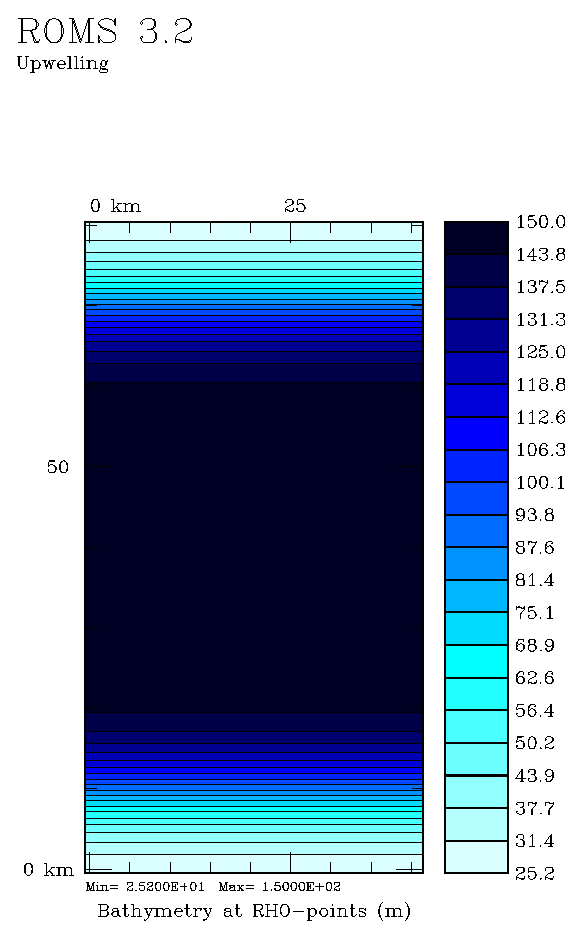
\includegraphics{pics/up1}
\end{picture}
\caption{The upwelling/downwelling bathymetry.}
\label{fsm1}
\end{figure}

\begin{figure}
\setlength{\unitlength}{10mm}
\begin{picture}(0,16)(-3.75,0)
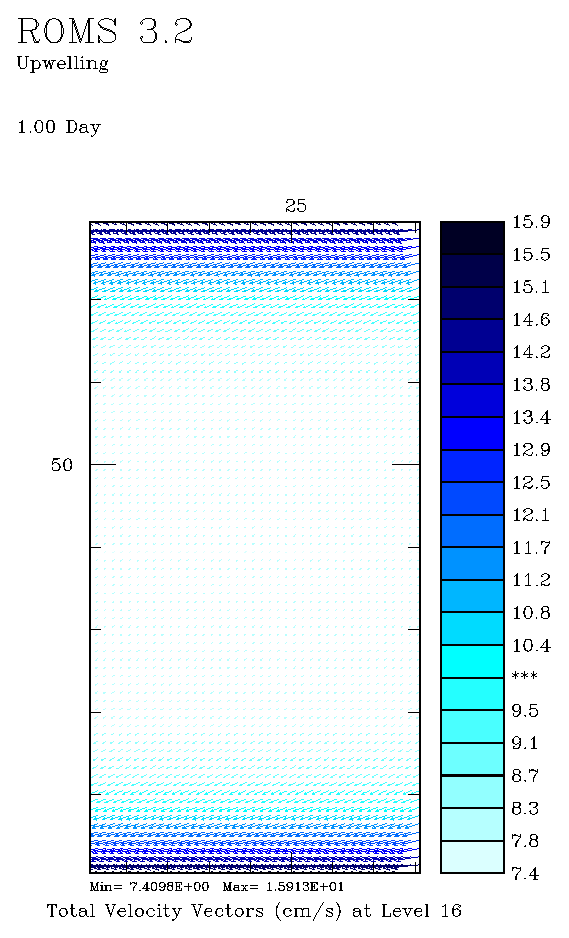
\includegraphics{pics/up2}
  \end{picture}
\caption{Surface velocities after one day, showing the flow to the
left of the wind (southern hemisphere).}
\end{figure}

\begin{figure}
\setlength{\unitlength}{10mm}
\begin{picture}(0,16)(0,0)
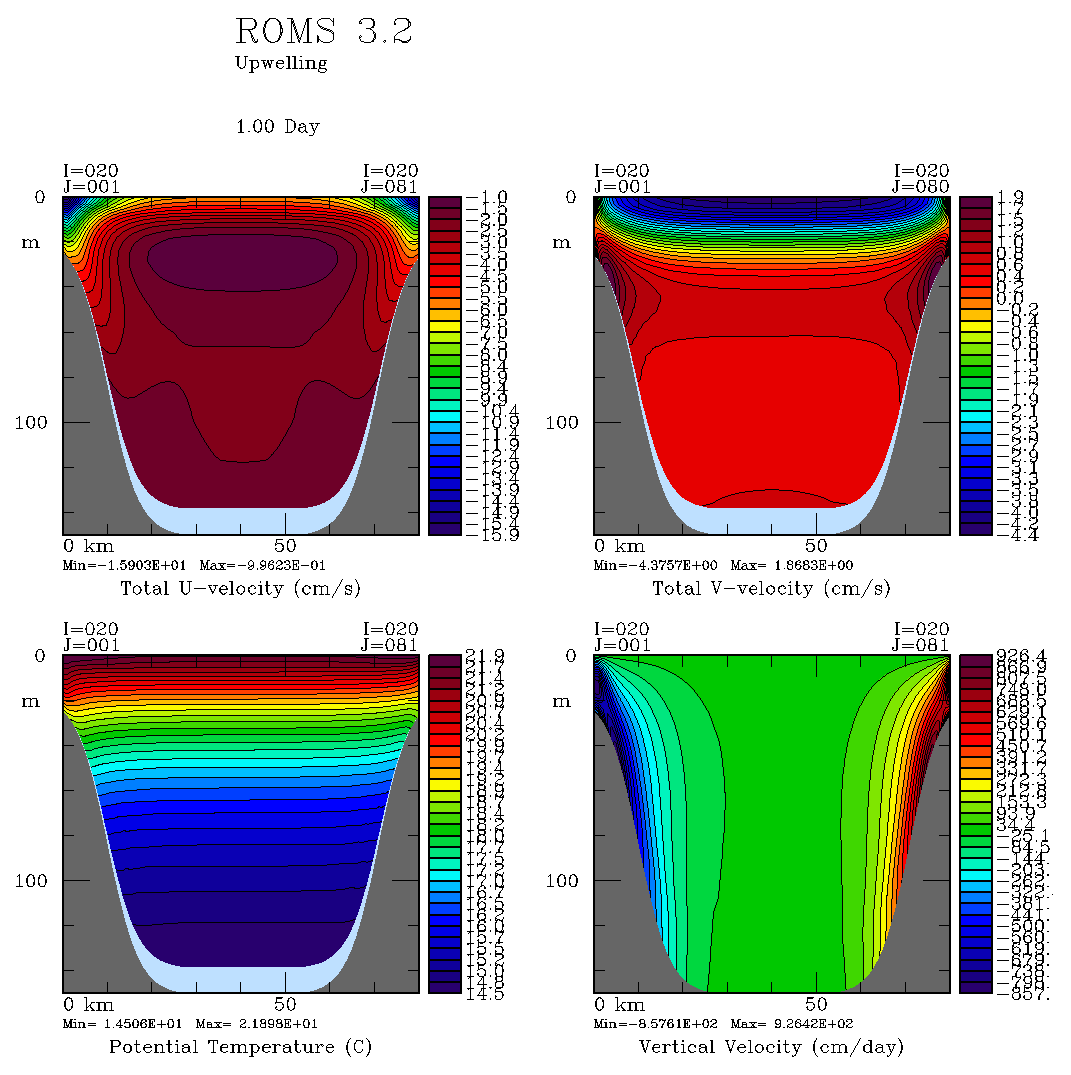
\includegraphics[width=6.5in]{pics/up3}
  \end{picture}
\caption{Constant $\xi$ slices of the $u, v, T$ and $w$ fields
at day 1.}
\end{figure}

\begin{figure}
\setlength{\unitlength}{10mm}
\begin{picture}(0,16)(0,0)
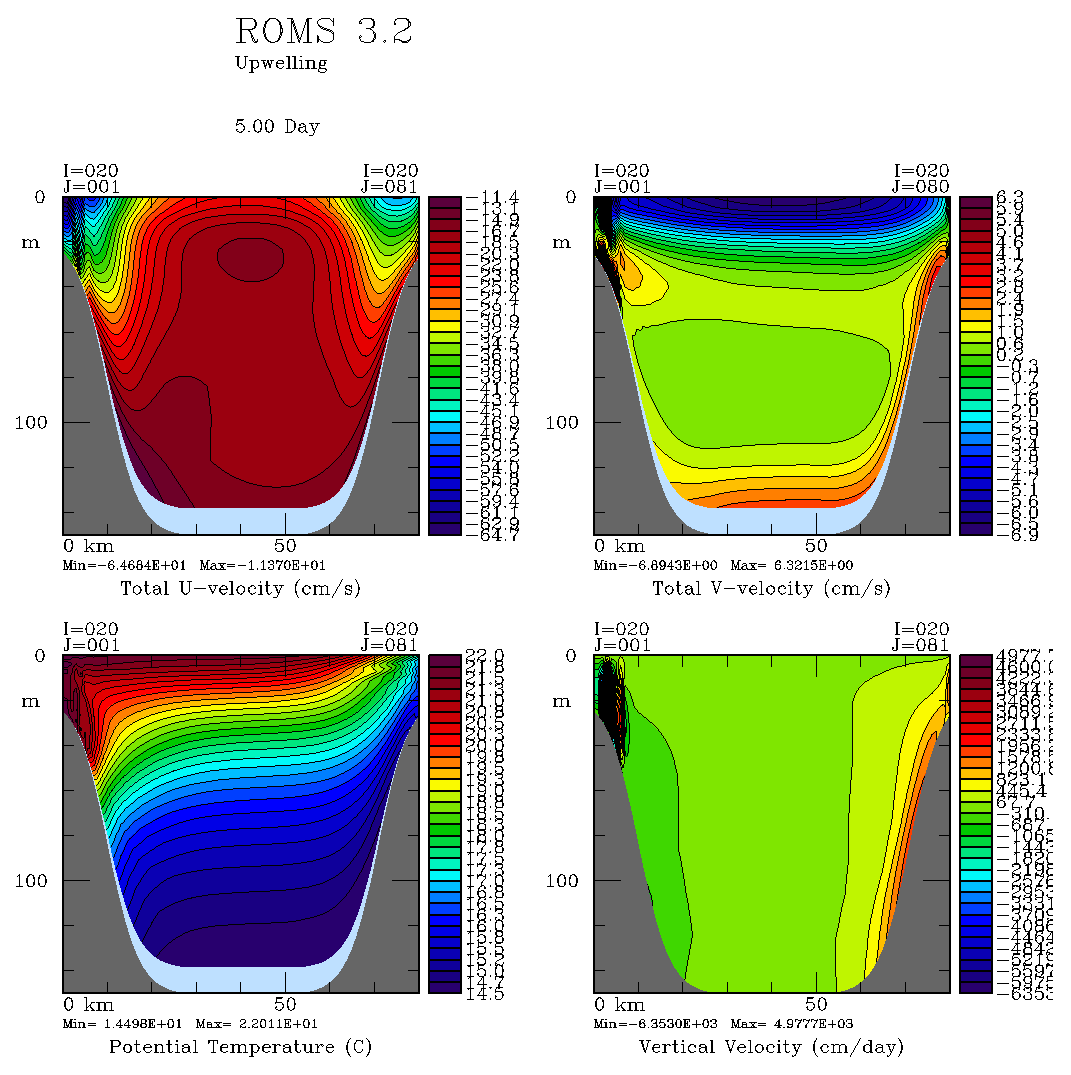
\includegraphics[width=6.5in]{pics/up4}
  \end{picture}
\caption{Constant $\xi$ slices of the $u, v, T$, and $w$ fields
at day 5.}
\label{fsm2}
\end{figure}

\subsection{Arctic example}
\label{ARCTIC}
The upwelling/downwelling examples is one in which all the start-up
fields are defined analytically.  The other extreme is one in which
everything is read from files, as in our Arctic simulations.
Figure \ref{fbath_arc} shows the bathymetry and the extent of this
domain. The grid is non-uniform, having more resolution close to
Alaska - a measure of grid spacing is shown in Figure
\ref{fgspace_arc}.

\begin{figure}
\setlength{\unitlength}{10mm}
\begin{picture}(0,16)(0,0)
\includegraphics{pics/bath_Arc}
  \end{picture}
\caption{Bathymetry of the Arctic domain.}
\label{fbath_arc}
\end{figure}

\begin{figure}
\setlength{\unitlength}{10mm}
\begin{picture}(0,16)(0,0)
\includegraphics{pics/size_Arc}
  \end{picture}
\caption{Grid spacing of the Arctic domain.}
\label{fgspace_arc}
\end{figure}

\subsubsection{\code{arctic.h}}
The C preprocessor variable \code{ARCTIC} has been chosen to
label our Arctic domain, which is a close cousin to \code{NEP6}.
The header include file then becomes \code{arctic.h}:
\begin{verbatim}
/*
** svn $Id$
*******************************************************************************
** Copyright (c) 2002-2012 The ROMS/TOMS Group
**
**   Licensed under a MIT/X style license
**
**   See License_ROMS.txt
**
*******************************************************************************
**
**  Options for ARCTIC simulation
*/

#define NO_HIS
#define GLOBAL_PERIODIC
#undef NETCDF4
#undef PARALLEL_IO
#undef OFFLINE_FLOATS

/* general */

#define CURVGRID
#define MASKING
#define NONLIN_EOS
#define SOLVE3D
#define SALINITY
#ifdef SOLVE3D
# define SPLINES
#endif
#define FLOATS
#define STATIONS
#undef WET_DRY

#undef T_PASSIVE
#ifdef T_PASSIVE
# define ANA_PASSIVE
# define TRC_PSOURCE
# define ANA_TRC_PSOURCE
# define AGE_PASSIVE
#endif
 
/* ice */

#ifdef SOLVE3D
# define  ICE_MODEL
# ifdef ICE_MODEL
#  define  OUTFLOW_MASK
#  define  FASTICE_CLIMATOLOGY
#  define  ICE_THERMO
#  define  ICE_MK
#  undef   ICE_ALB_EC92
#  undef   ICE_SMOOTH
#  define  ICE_MOMENTUM
#  define  ICE_MOM_BULK
#  define  ICE_EVP
#  define  ICE_ADVECT
#  define  ICE_SMOLAR
#  define  ICE_UPWIND
#  define  ICE_BULK_FLUXES
#  undef  ANA_AIOBC
#  undef  ANA_HIOBC
#  undef  ANA_HSNOBC
# endif
#endif

/* output stuff */
 
#define NO_WRITE_GRID
#undef OUT_DOUBLE
#define RST_SINGLE
#define AVERAGES
#define AVERAGES2
#ifdef SOLVE3D
# undef AVERAGES_DETIDE
# undef DIAGNOSTICS_TS
#endif
#undef DIAGNOSTICS_UV
 
/* advection, dissipation, pressure grad, etc. */
 
#ifdef SOLVE3D
# define DJ_GRADPS
#endif
 
#define UV_ADV
#define UV_COR
#undef UV_SADVECTION
 
#ifdef SOLVE3D
# define TS_U3HADVECTION
# define TS_C4VADVECTION
# undef TS_MPDATA
#endif
 
#define UV_VIS2
#undef UV_SMAGORINSKY
#undef VISC_3DCOEF
#define MIX_S_UV
#define VISC_GRID
#undef SPONGE

#ifdef SOLVE3D
# define TS_DIF2
# define MIX_GEO_TS
# define DIFF_GRID
#endif
 
/* vertical mixing */
 
#ifdef SOLVE3D
# define SOLAR_SOURCE
# define WTYPE_GRID
 
# undef LMD_MIXING
# ifdef LMD_MIXING
#  define LMD_RIMIX
#  define LMD_CONVEC
#  define LMD_SKPP
#  undef LMD_BKPP
#  define LMD_NONLOCAL
#  define LMD_SHAPIRO
#  undef LMD_DDMIX
# endif
 
# define GLS_MIXING
# undef MY25_MIXING

# if defined GLS_MIXING || defined MY25_MIXING
#  define KANTHA_CLAYSON
#  define N2S2_HORAVG
# endif
#endif
 
/* surface forcing */
 
#ifdef SOLVE3D
# define BULK_FLUXES
# define CCSM_FLUXES
# if defined BULK_FLUXES || defined CCSM_FLUXES
#  define LONGWAVE_OUT
#  define DIURNAL_SRFLUX
#  define EMINUSP
#  undef ANA_SRFLUX
#  undef ALBEDO
#  define ALBEDO_CURVE
#  undef LONGWAVE
# endif
#endif
 
/* surface and side corrections */
 
#ifdef SOLVE3D
# define SCORRECTION
# undef QCORRECTION
# undef TCLIMATOLOGY
# undef TCLM_NUDGING
#endif
 
/* point sources (rivers, line sources) */
 
/* Using Runoff instead now */
#ifdef SOLVE3D
#define RUNOFF
# define UV_PSOURCE
# define ANA_PSOURCE
# undef TS_PSOURCE
#endif
 
/* tides */
 
#define LTIDES
#ifdef LTIDES
# define FILTERED
# define SSH_TIDES
# define UV_TIDES
# define ADD_FSOBC
# define ADD_M2OBC
# undef RAMP_TIDES
# define TIDES_ASTRO
# define POT_TIDES

# define UV_LDRAG
# define UV_DRAG_GRID
# define ANA_DRAG
# define DRAG_LIMITER
# undef UV_QDRAG
#else
# define UV_QDRAG
#endif
 
/* Boundary conditions...careful with grid orientation */
 
#define RADIATION_2D
 
/* roms quirks */
 
#ifdef SOLVE3D
# define ANA_BSFLUX
# define ANA_BTFLUX
#else
# define ANA_SMFLUX
#endif

/*
**  Biological model options.
*/
#undef NEMURO

#if defined NEMURO
# define BIO_SEDIMENT
# define NEMURO_SED1
# undef ANA_BIOLOGY       /* analytical biology initial conditions */
# define ANA_BPFLUX        /* analytical bottom passive tracers fluxes */
# define ANA_SPFLUX        /* analytical surface passive tracers fluxes */
# define IRON_LIMIT        /* Add iron as passive 11th tracer */
# define IRON_RELAX
# undef  IRON_RSIN
# define HOLLING_GRAZING
# undef  IVLEV_EXPLICIT
# undef  ANA_BIOSWRAD
# undef  DIAGNOSTICS_BIO
#endif
\end{verbatim}
We've got masking, salinity, sea ice and the non-linear equation of state.
We want Laplacian viscosity on $\sigma$-surfaces, diffusion along constant
$z$-surfaces and the full non-linear, curvilinear momentum equations.

Notice that comments are allowed in this file as long as they are in
the C/C++ syntax. Also, conditionals are fine---some parts are only
wanted when \code{SOLVE3D} is on. There is evidence of options
having been tried and rejected, such as the quadratic bottom drag
in the presence of tides.
Sources are turned on to presribe inflow through Bering Strait
(\code{UV\_PSOURCE}).

\subsubsection{Arctic code chunks}
The \code{Apps/Arctic} directory contains the \code{ana\_}
family of include files for setting the bottom drag, the horizontal
mixing coefficients, and the nudging coefficients.
Doing a search for \code{ARCTIC} shows up a few other bits of code. One
is in \code{output.F}, forcing a new station file after every
restart:
\begin{verbatim}
#ifdef ARCTIC
          CALL def_station (ng, .true.)
#else
          CALL def_station (ng, ldefout(ng))
#endif
\end{verbatim}
A better fix (someday) would be to allow the station files to be
numbered just like the averages files. Why not set \code{ldefout} to
be true? It is shared by many outputs, including the floats, and you
can only restart floats with \code{ldefout} set to false.

There is a hack in \code{grid\_coords.F} so that floats and stations
are placed at the correct $i,j$ position. Otherwise, the code to
find $i,j$ from longitude, latitude finds two boxes with the correct
range, one where I want it, the other at the same latitude, but
where the longitude jumps from 360 back to 0.

There is code in \code{set\_masks.F} to position the mask for
the ice outflow cells off the coast of Greenland.

Finally, there is a kludge in \code{step\_floats.F} for a
float reuse strategy, restarting them each year. Having a handy tag like
\code{ARCTIC} allows me to search for these little hacks later.

\subsubsection{Model domain}
A number of horizontal grid points was chosen to resolve the
domain at roughly 5 km near Alaska, less well across the basin, but
with only twice as many points as the regional Chukchi domain. Values
for \code{Lm}, \code{Mm}, and \code{N} are:
\begin{verbatim}
          Lm == 472           ! Number of I-direction INTERIOR RHO-points
          Mm == 480           ! Number of J-direction INTERIOR RHO-points
           N == 50            ! Number of vertical levels
\end{verbatim}
The vertical structure is set to our new favorite, using the new stretching:
\begin{verbatim}
  Vtransform == 2                          ! transformation equation
 Vstretching == 4                          ! stretching function

     THETA_S == 7.0d0                      ! surface stretching parameter
     THETA_B == 2.0d0                      ! bottom  stretching parameter
      TCLINE == 250.0d0                    ! critical depth (m)
\end{verbatim}

\subsubsection{Initial and boundary conditions}
The best ocean fields we knew of when setting this up are known as SODA, a
reanalysis from 1958 through 2005 by
\citet{Carton_2005}. There are \code{Python} scripts to create
initial and boundary conditions from the SODA files. Snow and ice
initial and boundary conditions are obtained from model results generously
provided by Jinlun Zhang. I am using three boundary files so that each
field can have its own unlimited dimension---there are three frequencies,
from daily to monthly.

The side known as ``South'' is along Northern Alaska and Western
Canada and is set to closed. The side known as ``West'' is only open
at Bering Strait, where I am imposing the inflow using a ``rivers''
file, but letting temperature and salinity come in from SODA
boundary conditions. The last two boundaries on the Atlantic side
have our usual combination of radiation and nudging:
\begin{verbatim}
   LBC(isFsur) ==   Cha     Clo     Cha     Cha         ! free-surface
   LBC(isUbar) ==   Clo     Clo     Fla     Fla         ! 2D U-momentum
   LBC(isVbar) ==   Clo     Clo     Fla     Fla         ! 2D V-momentum
   LBC(isUvel) ==   Clo     Clo     RadNud  RadNud      ! 3D U-momentum
   LBC(isVvel) ==   Clo     Clo     RadNud  RadNud      ! 3D V-momentum
   LBC(isMtke) ==   Gra     Clo     Gra     Gra         ! mixing TKE

   LBC(isTvar) ==   RadNud  Clo     RadNud  RadNud \    ! temperature
                    RadNud  Clo     RadNud  RadNud      ! salinity

! Ice boundary conditions

   LBC(isAice) ==   Mix     Clo     Mix     Mix         ! ice concentration
   LBC(isHice) ==   Mix     Clo     Mix     Mix         ! ice thickness
   LBC(isHsno) ==   Mix     Clo     Mix     Mix         ! snow thickness
   LBC(isTice) ==   Clo     Clo     Clo     Clo         ! ice temperature
   LBC(isSfwat)==   Clo     Clo     Clo     Clo         ! surface water
   LBC(isSig11)==   Clo     Clo     Clo     Clo         ! sigma-11
   LBC(isSig12)==   Clo     Clo     Clo     Clo         ! sigma-12
   LBC(isSig22)==   Clo     Clo     Clo     Clo         ! sigma-22
   LBC(isUice) ==   Gra     Clo     Gra     Gra         ! ice U-momentum
   LBC(isVice) ==   Gra     Clo     Gra     Gra         ! ice V-momentum

\end{verbatim}

\subsubsection{Forcing}
We are using the CORE2 forcing files \citep{Large_08} and computing the
momentum, heat and salt fluxes from the atmospheric conditions and the
model's surface temperature. There are two options, one provided by
\code{bulk\_flux.F} and the other provided by \code{ccsm\_flux.F}. We
are using the second. With minimal fussing, the CORE2 files
can be used as is, on their native grid, then interpolated by ROMS
internally to the domain at hand. Other forcings include a nudging
to sea surface salinity, runoff from Dai and Trenberth, a fastice
climatology from Andy Mahoney, Bering Strait flow estimated by Seth
Danielson using Rebecca Woodgate's mooring data, and tides from OTPS.

\subsubsection{ocean.in}
We use an internal time-step of 200 $s$ and an external time-step of 10
$s$. The horizontal viscosity and diffusion is:
\begin{verbatim}
        TNU2 == 5.0d0  5.0d0                    ! m2/s
       VISC2 == 25.0d0                          ! m2/s
\end{verbatim}

\subsubsection{Output}
The model writes voluminous information to standard out, as shown
for the \code{UPWELLING} case.  It also writes out NetCDF files for
restart, daily averages, three-hourly averages2, stations and floats.
Plots can be made from any of these files; some examples are shown
in Fig.\ \ref{fnep1}--\ref{fnep2} .

\begin{figure}
\setlength{\unitlength}{10 mm}
\begin{picture}(16,9)(0.0,0.4)
\includegraphics[width=16cm]{pics/usurf_Arc}
  \end{picture}
\caption{Surface velocity averaged over the month of June, 1986.}
\label{fnep1}
\end{figure}

\begin{figure}
\setlength{\unitlength}{10 mm}
\begin{picture}(16,12)(0.0,0)
\includegraphics[width=16cm]{pics/aice_Arc}
  \end{picture}
\caption{Ice concentration averaged over the month of June, 1986.}
\end{figure}

\begin{figure}
\setlength{\unitlength}{10 mm}
\begin{picture}(16,18)(0.0,0)
\includegraphics[width=16cm]{pics/float_Arc}
  \end{picture}
\caption{Five-day tracks of some surface floats, showing the starting
positions in blue.}
\label{fnep2}
\end{figure}


%%%%\section{Support Programs for Initialization}
\label{Progs}

Links to all the programs mentioned here are under the ROMS web site:
\begin{verbatim}
      http://marine.rutgers.edu/po/models/roms.html
\end{verbatim}

\subsection{Grid generation}
\label{Grid}
On startup, SCRUM either reads a NetCDF file or calls \code{ana\_grid}
and \code{ana\_mask}
to find the location of the grid points, the grid metrics,
the bathymetry, the land/sea mask, and the
Coriolis parameter $f$.  If you won't be using \code{ana\_grid}, the
grid file must be generated before SCRUM can be run, either with
the programs in \code{gridpak} or with \code{SEAGRID}.

%\subsubsection{\code{ezgrid}}
%\label{Ez}
%\code{ezgrid} was written to generate a uniform rectangular grid
%with a simple bathymetry.  It has two modes, one for the upwelling
%example, and one for rectangular basins; the mode is determined by
%the \code{UPWELLING} switch in \code{cppdefs.h}.  If \code{UPWELLING}
%is not defined then the important parameters are:
%\begin{klist}
%   \kitem{xl}   basin length in the $\xi$-direction.
%   \kitem{el}   basin width in the $\eta$-direction.
%   \kitem{h0}   bottom depth.
%   \kitem{f0, beta}  Coriolis parameter with the $\beta$-plane
%   approximation, $f = f_o + \beta y$.
%\end{klist}
%In either case you will have to also set the name of the gridfile,
%\code{grdname}, near the top of the \code{ezgrid.F} file.
%Once these parameters are set to your chosen values, compile and run it:
%\begin{verbatim}
%        make ezgrid
%        ezgrid
%\end{verbatim}
%This should create a binary NetCDF file called \code{grdname}.

\subsubsection{\code{gridpak}}
SCRUM has been designed to be used with curvilinear orthogonal grids
for boundary-following domains, etc., so there are situations in which
you want a more flexible grid-generation program than \code{ezgrid}.
We have been working on a suite of programs called \code{gridpak},
including \code{xcoast}, an interactive boundary drawing program.
See above for instructions on obtaining \code{gridpak}
and its documentation.

\subsection{Masking}
\label{Mask}
\subsubsection{The \code{scrum\_mask} program}
SCRUM now supports the masking of land areas, for which it requires
some new input arrays.  These arrays are read from the grid NetCDF
file or computed in \code{ana\_mask}.
The mask is defined on $\rho$-points; see Fig.\ \ref{fmask} for an
example of a small domain with an
isolated island and a promontory adjacent to the boundary.
\begin{figure}[thb]
  \setlength{\unitlength}{0.0125in}%
  \begin{picture}(0,0)(-138,-18)%
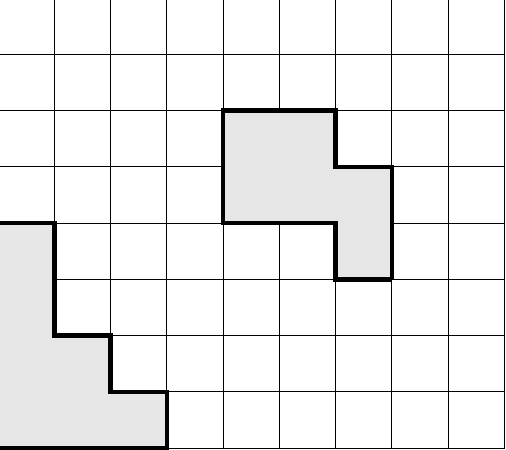
\includegraphics{pics/mask.pdf}%
  \end{picture}%
  \begin{picture}(300,264)(-9,461)
  \put(384,462){\makebox(0,0)[lb]{$i=\code{L}$}}
  \put(114,462){\makebox(0,0)[lb]{$i=1$}}
  \put( 93,477){\makebox(0,0)[lb]{$j=1$}}
  \put( 90,714){\makebox(0,0)[lb]{$j=\code{M}$}}
  \end{picture}
\caption{Small grid with masked regions}
\label{fmask}
\end{figure}
There are also arrays for the mask on $u$-points, $v$-points, and
$\psi$-points which are derived from the $\rho$-point mask.  The
$\psi$-point mask depends on the free-slip/no-slip option chosen
as described in \S\ref{Mask1}.

The programs in \code{gridpak} find the $\rho$-point mask based on the
bathymetry dataset.  Elevations at or above sea level are assumed to be
in the land mask.  You may choose to edit this mask, so Hernan Arango
has written a \code{Matlab} tool called \code{edit\_mask}.  It is an
interactive tool which requires \code{Matlab} as well as \code{mexnc}
for reading and writing NetCDF files from \code{Matlab}. On startup,
it will pop up file browsers, first for the grid file, then for a
coastline file. See Fig.\ \ref{fmat0} showing the file browser.

The view it presents is always rectangular, even for curvilinear grids,
but it will compute the coastline in the same (possibly) warped view to
allow a comparison. The first time you run it, it saves this mapped
coastline file to \code{ijcoast.mat} in the current directory.
Coastlines can be obtained from ...

\begin{figure}[pt]
  \setlength{\unitlength}{1 cm}%
  \begin{picture}(0,10)(0,0)%
\includegraphics{pics/edit_mask0.png}
  \end{picture}
\caption{The \code{edit\_mask} file browser.}
\label{fmat0}
\end{figure}

An example of its use is shown in
Fig.\ \ref{fmat}, showing a Bering Sea grid.
It displays a rectangle for each $\rho$-point, including the
boundary ``image'' points.  The green/yellow boxes are land while the blue
ones are ocean. Figure \ref{fmat2} shows a zoomed in view where you
can actually see the individual boxes. Notice that scroll bars
appear automatically, allowing you to pan around.

Advice for masking details are as follows:
\begin{itemize}
  \item Make the ``image'' points have the same mask value as the points
they mirror. Something to avoid is an ocean image point adjacent
to a land point along an open boundary.
  \item Avoid one-grid bays such as the one that got away and is in
the right side of Fig.\ \ref{fmat2}. While these shouldn't cause the
model any direct grief, most plotting software cannot show you what
is happening in such places.
\end{itemize}

\begin{figure}[p]
  \setlength{\unitlength}{1 cm}%
  \begin{picture}(0,14)(0,0)%
\includegraphics{pics/edit_mask1.png}
  \end{picture}
\caption{The \code{edit\_mask} program in action.}
\label{fmat}
\end{figure}

\begin{figure}[p]
  \setlength{\unitlength}{1 cm}%
  \begin{picture}(0,14)(0,0)%
\includegraphics{pics/edit_mask2.png}
  \end{picture}
\caption{The \code{edit\_mask} program zoomed in.}
\label{fmat2}
\end{figure}

\subsection{Objective Analysis}
\label{OA}
[This section was contributed by Hernan Arango.]

The objective analysis (\code{oa}) package described here can be used
to prepare initial, climatology, update,  and forcing fields for SCRUM.
It maps oceanographic and atmospheric data to a specified application
grid.  Currently, it processes the following fields: {\sl in situ}
temperature, potential temperature, {\sl in situ} density anomaly,
salinity, sigma-t, sound speed, dynamic height, surface net heat flux
($Q$), surface freshwater flux, precipitation rate, evaporation rate,
incoming solar shortwave radiation, surface momentum (wind) stress
components, sea surface temperature (SST), and surface net heat flux
sensitivity to SST ($\partial Q / \partial {\rm SST}$).

This \code{oa} package is derived from an earlier program which Hernan
Arango and Carlos Lozano wrote at Harvard University in 1993.   The
basic algorithm used by this package is described in
\cite{Carter87}.  A comprehensive description of this
methodology can also be found in \cite{Gandin63},
\cite{Bretherton76}, \cite{McWilliams86},
\cite{Daley91}, \cite{Bennett92}, and others.

Given observations $s_i = s({\bf x}_i, t_i)$ at location ${\bf x}_i,
t_i, i = 1, \ldots N$ an estimate $\phi_E$ of a scalar $\phi$ is
derived for location ${\bf x}$ and time $t$.  A linear unbiased estimate
is given by:
\[
   \phi_E({\bf x}, t) = \overline{\phi}({\bf x},t) + \sum_i w_i (s_i -
   \overline{s_i})
\]
for arbitrary $w_i$ since $\overline{\phi_E} = \overline{\phi}$.  The
associated variance of error is:
\[
  \overline{e^2(w)} = \overline{(\phi - \phi_E(w))^2}
\]
with $w = (w_1, \ldots w_N)$.  The overbar denotes an expected or
ensemble mean value.  The minimizer $w_*$:
\[
   \overline{e^2 (w_*)} \leq \overline{e^2(w)}
\]
is
\[
   w_* = {\bf A}^{-1} p
\]
with minimum error variance (Gauss-Markov):
\[
   \overline{e}^2_* = \overline{e^2(w_*)} = \overline{(\phi -
   \overline{\phi})^2} - p' {\bf A}^{-1} p
\]
Here, for convenience, matrix notation has been used.  $s = [s_1, \ldots
s_N]$ is a column correlation vector, $p = (\phi - \overline{\phi})(s
- \overline{s})$, and ${\bf A}$ is the covariance matrix:
\[
   {\bf A} = \overline{(s - \overline{s})(s - \overline{s})'}
\]
where the prime denotes a transpose.

Notice that ${\bf A}$ is symmetric.  In what follows, excluding
pathological cases, ${\bf A}$ is assumed to be positive definite.
The best linear estimate $\phi_*$ is then:
\[
   \phi_*({\bf x}, t) = \overline{\phi({\bf x}, t)} + p' {\bf A}^{-1}
   (s - \overline{s})
\]
with error $\overline{e^2_*}$.

The essential information required is statistical; namely the
spatial-temporal mean of the scalar and observations, the covariance
between observations, and the covariance between the scalar and the
observations.

The observations can be of different types, and different from the
scalar which you are trying to find.  Their usefulness is measured
by the fractional reduction of error:
\[
    {p'{\bf A}^{-1} p \over \overline{(\phi - \overline{\phi})^2}}
\]
In this package it is assumed that the covariance of the scalar is
homogeneous in space and homogeneous and isotropic in time:
\[
   C \left( ({\bf x_1}, t_1), ({\bf x_2}, t_2) \right) = 
   C \left( {\bf x_1 - x_2}, \left| t_2 - t_1 \right| \right)
\]
and errors at two different locations and times are uncorrelated:
\[
   E \left( ({\bf x}_1, t_1), ({\bf x}_2, t_2) \right) =
   E ({\bf x}_1, t_1) \delta ({\bf x_2 - x_1}) \delta(t_2 - t_1) .
\]
Currently, an analytical, isotropic, Gaussian correlation function is
assumed:
\[
    C({ \bf x_1 - x_2}, |t_2 - t_1| ) =
    {\cal C} ( |{ \bf x_1 - x_2}|, |t_2 - t_1| )
\]
with
\[
    {\cal C} ({\bf r}, \tau) = \exp \left[ - \left({\tau \over \tau_o}
    \right) ^2 \right] G({\bf r})
\]
\[
    G({\bf r}) = \left[ 1 - \left({{\bf r} \over a} \right)^2 \right]
    \exp \left[-\left({{\bf r} \over b} \right)^2 \right]
\]
where $\tau_o$ is the time decorrelation scale, $a$ is the zero
crossing distance, and $b$ is the spatial decorrelation scale.

This package uses a local solution to the \code{oa} equations.  That
is, only \code{nnce} influential observations are considered at each
mapped grid point.  This method is practical because it avoids
inverting large matrices when the number of observations is large.
Observations that are too far apart in space and time from the mapped
point contribute very little to the estimate, as one might expect.

\subsection{Forcing fields}
There are options for calling either \code{ana\_smflux} or
\code{get\_smflux} to get the surface momentum forcing.  If you do not
have an analytic formulation for this field,  you will have to create a
NetCDF forcing file which contains the surface momentum fluxes. This
file can be created with the \code{forcing} program, which reads the
output of the \code{oa} package.

The forcing file can
either contain one point value or a 2-D field of values.  Likewise, the
field can be constant in time or contain values for a series of times.
It is even possible to have a limited number of snapshots which get
cycled over in time.  For instance, you can provide 12 monthly mean
fields and tell it to cycle over these in a multi-year run.

The other forcing fields are treated in the same way and are also
contained in the NetCDF forcing file.  These include surface and bottom
heat and salt fluxes, the $\partial Q / \partial T$ and $T_{\rm ref}$
terms from \S\ref{vbc}, the incoming shortwave radiation used by the
Large et al.\ mixing scheme, and the wave information used by the
Styles and Glenn bottom boundary layer.  The ice thermodynamics also
requires forcing fields such as air temperature and cloud fraction.


\subsection{Initial and climatology fields}
The model will either read its initial fields from a NetCDF file or it
will compute them in \code{analytical.F}.  If it is not computing them,
the routine \code{get\_initial} will read a history file or a file
produced by the \code{initial} program.  This program in turn is
expecting to read the output of the \code{oa} program.

The model has the option of reading in 3-D climatology fields from a
climate NetCDF file.  This file contains the 3-D climatologies for the
tracers, perhaps at a number of times.  The subroutine \code{get\_clima}
will read this file and do any necessary time interpolations.  The
climate file is also produced by the \code{initial} program.  The
climatology could also be used for the boundary conditions, both for
the tracer values on inflow or for prescribed boundary conditions.  In
this case it would make more sense to only store the 2-D arrays.  We do
not yet have the software for handling these 2-D arrays, but it would
be a straightforward modification to the \code{initial} program.

%\include{floats}
%\section{Plotting Programs for Postprocessing}
\label{Plothist}
Hernan Arango has provided SCRUM with some programs for creating plots
from the NetCDF history and restart files. Some example plots are shown
in \S\ref{Wave}. There are four plotting programs:
\begin{klist}
   \kitem{cnt} creates black-and-white plots of the horizontal fields,
including constant depth plots of the 3-D fields.
   \kitem{ccnt} creates color plots of the horizontal fields,
including constant depth plots of the 3-D fields.
   \kitem{sec} creates black-and-white plots of vertical slices through
the 3-D fields.  It includes on option of finding equal-spaced points
along a straight line through the curvilinear grid.
   \kitem{csec} creates color plots of vertical slices through
the 3-D fields.  It includes on option of finding equal-spaced points
along a straight line through the curvilinear grid.
\end{klist}
All of these program come with example input files.  For instance, the
input file for \code{ccnt} is called \code{ccnt.in} and is as follows:
\begin{verbatim}
1996 -1  :  year and starting year-day (use yearday<0, for no time label)
SCRUM 3.0
Coarse Arctic ocean with Budgell ice dynamics
ice thermodynamics

8     NFIELDS: number of fields to plot. Line below, field(s) types:
42,45,46,47,48,49,50,121,122,123,124  field identification:
FLDID(1:NFIELDS)
1     NLEVELS: number of levels and/or depths to plot (0 for all levels)
20           levels (>0) or depths (<0) to plot: FLDLEV(1:NLEVELS)
2     NFIELDS: number of fields to plot. Line below, field(s) types:
1,2            field identification: FLDID(1:NFIELDS)
1     NLEVELS: number of levels and/or depths to plot (0 for all levels)
1,2,3,4,5      levels (>0) or depths (<0) to plot: FLDLEV(1:NLEVELS)
0     FRSTD  : first day to plot
0     LASTD  : last day to plot
0     DSKIP  : plot every other DSKIP days (0.0 plot at its own time frequency)
0     VINTRP : vertical interpolation scheme: 0=linear, 1:cubic splines
0.0   PMIN   : field minimum value for color palette (0.0 for default)
0.0   PMAX   : field maximum value for color palette (0.0 for default)
1     ICNT   : draw contours between color bands: 0=no, 1=yes
0.0   ISOVAL : iso-surface value to process (see below)
1.2   VLWD   : vector line width (1.0 for default)
2.0   VLSCL  : vector length scale (1.0 for default)
1     IVINC  : vector grid sampling in the X-direction (1 for default)
1     JVINC  : vector grid sampling in the Y-direction (1 for default)
0     IREF   : secondary or reference field option (see below)
25    IDOVER : overlay field identification (for IREF=1,2 only)
1     LEVOVER: level of the overlay field (set to 0 if same as current FLDLEV)
0.0   RMIN   : overlay field minimum value to consider (0.0 for default)
0.0   RMAX   : overlay field maximum value to consider (0.0 for default)
10.0   LGRID : Desired longitude/latitude grid spacing (degrees)
4     IPROJ  : map projection (see below).
-60.0   PLON : projection Pole longitude (west values are negative).
90.0   PLAT  : projection Pole latitude (south values are negative).
0.0   ROTA   : projection rotation angle (clockwise; degrees).
0     LMSK   : flag to color mask land: [0] no, [1] yes
-1     NPAGE : number of plots per page (currently 1, 2, or 4)  
T     READGRD: logical switch to read in positions from grid NetCDF file.
F     PLTLOGO: logical switch draw Logo.
T     WRTHDR : logical switch to write out the plot header titles.
T     WRTBLAB: logical switch to write out the plot bottom title.
T     WRTRANG: logical switch to write out data range values and CI.

T     WRTFNAM: logical switch to write out input primary filename.
T     WRTDATE: logical switch to write out current date.
T     CST    : logical switch to read and plot coastlines and islands.
50.0 50.0    : bottom and top map latitudes (south values are negative).
-110.0 80.0  : left and right map longitudes (west values are negative).
/d2/kate/plot/varid.dat
/d1/arango/scrum3.0/plot/Palettes/gs1.pal
/d2/kate/plot/default.cnt
ice_rst.nc
scrum_rst_1.nc
/d2/kate/arctic/gridpak/arctic_grid_2.nc
/u1/coasts/coast.dat


c
c=======================================================================
c  Copyright (c) 1996 Rutgers University                             ===
c=======================================================================
c

 *** Above FILENAMES:

            1st line: input; variables ID file.
            2nd line: input; color palette file.
            3rd line: input; contour parameters.
            4th line: input; primary NetCDF file.
            5th line: input; secondary NetCDF file.
            6th line: input; grid NetCDF file.
            7th line: input; coastlines file.

 *** IREF:  Secondary or reference field option:
           -1   Overlay horizontal grid
            0   no secondary or reference field to plot
            1   plot field overlay from primary file
            2   plot field overlay from secondary file
            3   primary - secondary file (field subtraction)
            4   Day0 - DayN (field subtraction)

 *** IPROJ: Map Projections option.  Some of the values for the
            projection Pole and rotation angle are suggested.
            Check the NCAR manual for details.

           [1] Cylindrical equidistant: PLON=0, PLAT=0, ROTA=0
           [2] Mercator: PLON=?, PLAT=0, ROTA=0
           [3] Lambert conformal conic: PLON=?, PLAT=?, ROTA=?
           [4] Stereographic azimuthal:  PLON=?, PLAT=90 or -90, ROTA=0

 *** IVINC, JVINC: vector grid sampling.  If either value is negative,
                   the velocity vectors at drawn at PSI-points.  Otherwise,
                   if both values are positive, the vectors are drawn at
                   interior RHO-points.

 *** LGRID: Longitude/latitude grid spacing.  The grid is drawn at
            LGRID spacing starting from specified map lower corner.
            If LGRID is negative, the latitude labels in the map are
            rotated 90 degrees to avoid label congestion, if any.

 *** NPAGE: Number of plots per page.  Set this parameter to a negative
            value (-1, -2, or -4) to activate preservation of the plot
            aspect ratio.


  Plotting Fields classification: (* derived fields)

 [  1]  IDUTOT  total velocity component in the XI-direction (cm/s).
 [  2]  IDVTOT  total velocity component in the ETA-direction (cm/s).
*[  3]  IDTVEC  total velocity vectors (cm/s).
*[  4]  IDTMAG  total velocity vector magnitude (cm/s).
                 :
                 :
\end{verbatim}
As you can see, there are comments describing what needs to be
done.  Please see the variable ID file for the complete list of fields
which can be plotted---this list changes as Hernan adds the ability to
plot new fields. Also, check your default.cnt file for other vector and
contour parameters. The palette file includes two number systems, one
in the scale from 0 to 255 and the other from 0 to 1.
The SCRUM plotting uses the first while the SEOM plotting uses the
second.

\section{Ice Model Formulation}
\label{Iphys}

The sea-ice component of ROMS is a combination of the
elastic-viscous-plastic (EVP) rheology (Hunke and Dukowicz
\cite{Hunke97}, Hunke \cite{Hunke_2001}) and simple one-layer
ice and snow thermodynamics with a molecular sublayer under the ice
(Mellor and Kantha \cite{Mellor89}). It is tightly coupled, having
the same grid (Arakawa-C) and timestep as the ocean and sharing the same
parallel coding structure for use with MPI or OpenMP (Budgell
\cite{Budgell05}).

\subsection{Dynamics}
The momentum equations describe the change in ice/snow velocity due
to the combined effects of the Coriolis force, surface ocean tilt,
air and water stress, and internal ice stress:
(\ref{ist1}) and (\ref{ist2}):
\begin{align}
  M \frac{\partial u }{ \partial t}
 % + M \vec{v} \cdot \nabla u
 & = Mfv - Mg \frac{\partial \zeta_w }{ \partial x} +
 \tau_a^x + \tau_w^x + {\cal F}_x
\label{ist1} \\
  M \frac{\partial v }{ \partial t}
 % + M \vec{v} \cdot \nabla v
 & = - Mfu - Mg \frac{\partial \zeta_w }{ \partial y} +
 \tau_a^y + \tau_w^y + {\cal F}_y.
\label{ist2}
\end{align}
In this model, we neglect the nonlinear advection terms as well as
the curvilinear terms in the internal ice stress.
Nonlinear formulas are used for both the ocean-ice and air-ice surface
stress:
\begin{align}
  \vec{\tau}_a & = \rho_a C_a | \vec{V}_{10} | \vec{V}_{10} \\
  C_a & = \frac{1 }{ 2} C_d \left[ 1 - \cos( 2 \pi \min(h_i+.1, .5)
  \right] \\
  \vec{\tau}_w & = \rho_w C_w | \vec{v}_w - \vec{v} |
  ( \vec{v}_w - \vec{v}) .
\end{align}
The force due to
the internal ice stress is given by the divergence of the stress
tensor $\sigma$. The rheology is given by the stress-strain relation
of the medium. We would like to emulate the viscous-plastic rheology
of Hibler (1979) \cite{Hibler79}:
\begin{equation}
  \sigma_{ij} = 2 \eta \dot \epsilon_{ij} + (\zeta - \eta) \dot
  \epsilon_{kk} \delta_{ij} - \frac{P }{ 2} \delta_{ij}
\end{equation}
\begin{equation}
  \dot \epsilon_{ij} \equiv \frac{1 }{ 2} \left( \frac{\partial u_i
  }{
  \partial x_j} + \frac{\partial u_j }{ \partial x_i} \right)
\end{equation}
\begin{equation}
  P = P^* A h_i e^{-C(1-A)}
\end{equation}
where the nonlinear viscosities are given by
\begin{equation}
\zeta = \frac{ P }{ 2 \left[ (\epsilon^2_{11} +
   \epsilon^2_{22} ) ( 1 + 1/e^2 ) + 4 e^{-2} \epsilon^2_{12}
      + 2 \epsilon_{11} \epsilon_{22} ( 1 - 1/e^2 ) \right] ^{1/2} }
\end{equation}
\begin{equation}
      \eta = \frac{ \zeta }{ e^2 }.
\end{equation}
We would also like to have an explicit model that can be solved
efficiently on parallel computers. The EVP rheology has a tunable
coefficient $E$ (the Young's modulus) which can be chosen to make
the elastic term small compared to the other terms. We rearrange the VP
rheology:
\begin{equation}
  \frac{1 }{ 2 \eta} \sigma_{ij} + \frac{\eta - \zeta }{ 4 \eta \zeta}
  \sigma_{kk} \delta_{ij} + \frac{P }{ 4 \zeta} \delta_{ij} = \dot
  \epsilon_{ij}
\end{equation}
then add the elastic term:
\begin{equation}
  \frac{1 }{ E} \frac{\partial \sigma_{ij} }{ \partial t} +
  \frac{1 }{ 2
  \eta} \sigma_{ij} + \frac{\eta - \zeta }{ 4 \eta \zeta} \sigma_{kk}
  \delta_{ij} + \frac{P }{ 4 \zeta} \delta_{ij} = \dot \epsilon_{ij}
\end{equation}

Much like the ocean model, the ice model has a split timestep. The
internal ice stress term is updated on a shorter timestep so as to
allow the elastic wave velocity to be resolved.

Once the new ice velocities are computed, the ice tracers can be
advected using the MPDATA scheme \cite{Smolark90}. The tracers in
this case are the ice thickness, ice concentration, snow thickness,
internal ice temperature, and surface melt ponds. The continuity
equations describing the evolution of these parameters (equations
(\ref{ist3a})--(\ref{ist3b})) also include thermodynamic terms ($S_h$,
$S_s$ and $S_A$), which will be described in \S\ref{Growth}:
\begin{align}
  \frac{\partial A h_i }{ \partial t} & =
  - \frac{\partial (u A h_i) }{ \partial x} -
  \frac{\partial (v A h_i) }{ \partial y}
  + S_h + {\cal D}_h
\label{ist3a} \\
  \frac{\partial A h_s }{ \partial t} & =
  - \frac{\partial (u A h_s) }{ \partial x} -
  \frac{\partial (v A h_s) }{ \partial y}
  + S_s + {\cal D}_s
\label{ist3c} \\
  \frac{\partial A }{ \partial t} & =
  - \frac{\partial (uA) }{ \partial x} - \frac{\partial (vA) }{ \partial y}
  + S_A + {\cal D}_A \qquad \qquad 0 \leq A \leq 1 .
\label{ist3b}
\end{align}
The first two equations represent the conservation of ice and snow.
Equation \ref{ist3b} is discussed in some detail in MK89, but
represents the advection of ice blocks in which no ridging occurs as
long as there is any open water. An optional ridging term can be added
(Gray and Killworth \cite{Gray96}):
\begin{equation}
  \frac{\partial A }{ \partial t} =
  - \frac{\partial (uA) }{ \partial x} - \frac{\partial (vA) }{ \partial y}
  - A \alpha(A) \, \nabla \cdot \vec{v} \, H(-\nabla \cdot \vec{v})
  + S_A + {\cal D}_A \qquad \qquad 0 \leq A \leq 1 .
\end{equation}
where $\alpha(A)$ is an arbitrary function such that $\alpha(0) = 0$,
$\alpha(1) = 1$, and $0 \leq \alpha(A) \leq 1$. The ridging term leads
to an increase in $h_i$ under convergent flow as would be produced by
ridging. The function $\alpha(A)$ should be chosen so that it is near
zero until the ice concentration is large enough that ridging is
expected to occur, then should increase smoothly to one.

The symbols used in these equations along with the values for the
constants are listed in Table \ref{icemomvars}.

\begin{table}[pt]
\hspace{9.5 mm}
\vbox{
\begin{tabular}{|c|c|l|} \hline
  Variable & Value & Description \\ \hline
  $A(x,y,t)$ && ice concentration \\
  $\alpha(A)$ && ridging function \\
  $C_a$ && nonlinear air drag coefficient \\
  $C_d$ & $2.2 \times 10^{-3}$ & air drag coefficient \\
  $C_w$ & $10 \times 10^{-3}$ & water drag coefficient \\
  (${\cal D}_h, {\cal D}_s, {\cal D}_A$) && diffusion terms \\
  $\delta_{ij}$ && Kronecker delta function \\
  $E$ && Young's modulus \\
  $e$ & 2 & eccentricity of the elliptical yield curve \\
  $\epsilon_{ij}(x,y,t)$ && strain rate tensor \\
  $\eta(x,y,t)$ && nonlinear shear viscosity \\
  $f(x,y)$ && Coriolis parameter \\
  (${\cal F}_x, {\cal F}_y$) && internal ice stress \\
  $g$  & $9.8\, m\, s^{-2}$ & acceleration of gravity \\
  $H$ &&  Heaviside function \\
  $h_i(x,y,t)$ && ice thickness of ice-covered fraction \\
  $h_o$ & 1 m & ice cutoff thickness \\
  $h_s(x,y,t)$ && snow thickness on ice-covered fraction \\
  $M(x,y,t)$ && ice mass (density times thickness) \\
  $P(x,y,t)$ && ice pressure or strength \\
  ($P^*, C$) & ($2.75 \times 10^4, 20$) & ice strength parameters \\
  ($S_h, S_s, S_A$) && thermodynamic terms \\
  $\sigma_{ij}(x,y,t)$ && stress tensor \\
  $\vec{\tau}_a$ && air stress \\
  $\vec{\tau}_w$ && water stress \\
  ($u,v$) && the ($x,y$) components of ice velocity $\vec{v}$ \\
  ($\vec{V}_{10}, \vec{v}_w$) &&
	      10 meter air and surface water velocities \\
  ($\rho_a, \rho_w$)  & ($1.3\, kg\, m^{-3}, 1025\, kg\, m^{-3}$) & air
  and water densities \\
  $\zeta(x,y,t)$ && nonlinear bulk viscosity \\
  $\zeta_w(x,y,t)$ && height of the ocean surface \\
  \hline
\end{tabular}
}
\caption{Variables used in the ice momentum equations}
\label{icemomvars}
\end{table}

Note that Hibler's $h_I$ variable is equivalent to our $A h_i$
combination - his $h_I$ is the average thickness over the whole
gridbox while our $h_i$ is the average thickness over the ice-covered
fraction of the gridbox. 

\subsection{Thermodynamics}
\label{Growth}

The thermodynamics is based on calculating how much ice grows and
melts on each of the surface, bottom, and sides of the ice floes,
as well as frazil ice formation (Mellor and Kantha \cite{Mellor89}).
Once the ice tracers are advected, the ice concentration and
thickness are timestepped according to the terms on the right:

(\ref{ist3a}) and (\ref{ist3b}) is:
\begin{align}
  \frac{D A h_i }{D t}
% + \frac{\partial (u A h_i) }{ \partial x} +
%  \frac{\partial (v A h_i) }{ \partial y}
  & = \frac{\rho_o }{ \rho_i} \left[ A (W_{io} - W_{ai}) + (1-A) W_{ao}
  + W_{fr} \right]
\label{ist4a} \\
  \frac{D A }{ D t}
%  +\frac{\partial (uA) }{ \partial x} + \frac{\partial (vA) }{ \partial y}
  & = \frac{\rho_o A }{ \rho_i h_i} \left[ \Phi (1-A) W_{ao} + (1-A)
  W_{fr} \right] \qquad \qquad 0 \leq A \leq 1 .
\label{ist4b}
\end{align}
The term $Ah_i$ is the "effective thickness", a measure of the ice
volume. Its evolution equation is simply quantifying the change in
the amount of ice. The ice concentration equation is more interesting in
that it provides the partitioning between ice melt/growth on the sides
vs. on the top and bottom. The parameter $\Phi$ controls this and has
differing values for ice melt and retreat. In principle, most of the ice
growth is assumed to happen at the base of the ice while rather more of
the melt happens on the sides of the ice due to warming of the water in
the leads.

The heat fluxes through the ice are based on a simple one layer
Semtner \cite{Semtner76a} type model with
snow on top. The temperature is assumed to be linear within the snow
and within the ice. The ice contains brine pockets for a
total ice salinity of 5. The surface ocean temperature and salinity
is half a $dz$ below the surface. The water right below the surface
is assumed to be at the freezing temperature; a logarithmic boundary
layer is computed having the temperature and salinity matched at
freezing.

Here, the $W$ variables are the freeze or
melt rates as shown in Fig.\ \ref{fm+k} and Table \ref{thermvar}.  The
frazil ice growth $W_{fr}$ will be discussed further in
\S\ref{frazil}---note that it contributes to changes in $A$ as well as
to changes in $h_i$.  The other term that contributes to $A$ is
$W_{ao}$.  This term includes a factor $\Phi$ which Mellor and Kantha
set to different values depending on whether ice is melting or
freezing:
\begin{align}
    \Phi & = 4.0 \qquad\qquad W_{ao} \geq 0 \\
    \Phi & = 0.5 \qquad\qquad W_{ao} < 0 \\
\end{align}

\begin{figure}[ht]
\setlength{\unitlength}{0.00083300in}%
%
%\begin{picture}(6527,2507)(270,-5042)
\begin{picture}(6527,2507)(885,-5042)
%\thicklines
\put(1501,-2911){\line( 1, 0){3975}}
\put(1501,-4111){\line( 1, 0){3975}}
\put(1501,-2911){\line( 0,-1){1200}}
\put(6976,-4111){\line( 1, 0){1050}}
\put(6976,-2911){\line( 1, 0){1050}}
\put(6976,-2911){\line( 0,-1){1200}}
\put(5476,-2911){\line( 0,-1){1200}}
\put(2401,-4861){\vector( 0, 1){750}}
\put(3376,-4861){\vector( 0, 1){750}}
\put(6226,-3586){\vector( 0, 1){675}}
\put(4426,-4036){\vector( 0,-1){525}}
\put(2596,-3376){\vector( 1, 1){450}}
%\put(1501,-5056){\framebox(6525,2505){}}
\put(6121,-3886){\makebox(0,0)[lb]{$W_{ao}$}}
\put(4336,-4756){\makebox(0,0)[lb]{$W_{ro}$}}
\put(2416,-3586){\makebox(0,0)[lb]{$W_{ai}$}}
\put(3241,-5056){\makebox(0,0)[lb]{$W_{io}$}}
\put(2296,-5056){\makebox(0,0)[lb]{$W_{fr}$}}
\end{picture}
%\begin{picture}(0,0)(5346,0)
\begin{picture}(0,0)(5961,0)
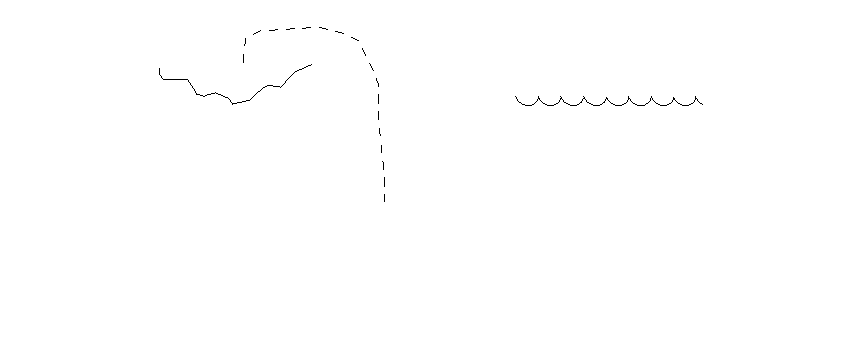
\includegraphics{pics/therm_mk}%
\end{picture}%
\caption{Diagram of the different locations where ice melting and
freezing can occur.}
\label{fm+k}
\end{figure}


\begin{table}
\hspace{9 mm}
\vbox{
\begin{tabular}{|c|c|l|} \hline
  Variable & Value & Description \\ \hline
  $\alpha_w$ & 0.10 & shortwave albedo of water \\
  $\alpha_i$ & 0.60 & shortwave albedo of wet ice \\
  $\alpha_i$ & 0.65 & shortwave albedo of dry ice \\
  $\alpha_s$ & 0.72 & shortwave albedo of wet snow \\
  $\alpha_s$ & 0.85 & shortwave albedo of dry snow \\
  $C_k$ && snow correction factor \\
  $C_{pi}$ & 2093 J kg$^{-1}$ K$^{-1}$ & specific heat of ice \\
  $C_{po}$ & 3990 J kg$^{-1}$ K$^{-1}$ & specific heat of water \\
  $\epsilon_w$ & 0.97 & longwave emissivity of water \\
  $\epsilon_i$ & 0.97 & longwave emissivity of ice \\
  $\epsilon_s$ & 0.99 & longwave emissivity of snow \\
  $E(T,r)$ && enthalpy of the ice/brine system \\
  $F_T\!\uparrow$ && heat flux from the ocean into the ice \\
  $H\!\downarrow$ && sensible heat \\
  $i_w$ && fraction of the solar heating transmitted \\
  && through a lead into the water below \\
  $k_i$ & 2.04 W m$^{-1}$ K${^-1}$ & thermal conductivity of ice \\
  $k_s$ & 0.31 W m$^{-1}$ K${^-1}$ & thermal conductivity of snow \\
  $L_i$ & 302 MJ m$^{-3}$ & latent heat of fusion of ice \\
  $L_s$ & 110 MJ m$^{-3}$ & latent heat of fusion of snow \\
  $LE\!\downarrow$ && latent heat \\
  $LW\!\!\downarrow$ && incoming longwave radiation \\
  $m$ & $-0.054^\circ$C/PSU & coefficient in linear $T_f(S) = mS$ equation \\
  $\Phi$ && contribution to $A$ equation from freezing water \\
  $Q_{ai}$ && heat flux out of the snow/ice surface \\
  $Q_{ao}$ && heat flux out of the ocean surface \\
  $Q_{i2}$ && heat flux up out of the ice \\
  $Q_{io}$ && heat flux up into the ice \\
  $Q_{s}$  && heat flux up through the snow \\
  $r$   && brine fraction in ice \\
  $\rho_i$ & 910 $m^3/kg$ & density of ice \\
  $S_i$ & 5 PSU & salinity of the ice \\
  $SW\!\!\downarrow$ && incoming shortwave radiation \\
  $\sigma$ & $5.67 \times 10^{-8}$ W m$^{-2}$ K$^{-4}$ &
  Stefan-Boltzmann constant \\
  $T_0$ && temperature of the bottom of the ice \\
  $T_1$ && temperature of the interior of the ice \\
  $T_2$ && temperature at the upper surface of the ice \\
  $T_3$ && temperature at the upper surface of the snow \\
  $T_f$ && freezing temperature \\
  $T_{{\rm melt}\_i}$ & $mS_i$ & melting temperature of ice \\
  $T_{{\rm melt}\_s}$ & 0$^\circ$ C & melting temperature of snow \\
  $W_{ai}$ && melt rate on the upper ice/snow surface \\
  $W_{ao}$ && freeze rate at the air/water interface \\
  $W_{fr}$ && rate of frazil ice growth \\
  $W_{io}$ && freeze rate at the ice/water interface \\
  $W_{ro}$ & $W_{ai}$ & rate of run-off of surface melt water \\
  \hline
\end{tabular}
}
\caption{Variables used in the ice thermodynamics}
\label{thermvar}
\end{table}

\begin{figure}
\centerline{
\begin{picture}(0,0)%
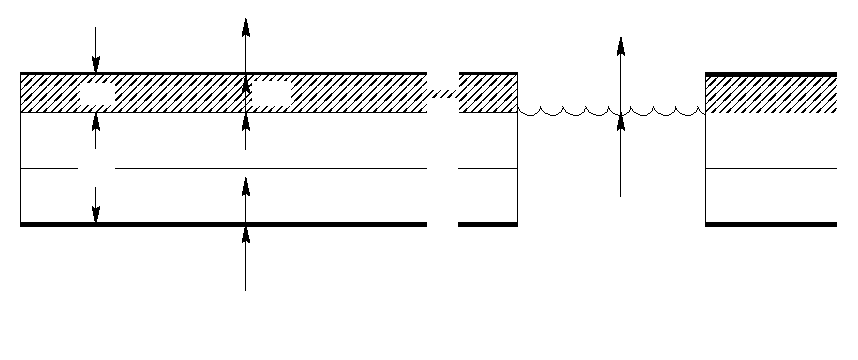
\includegraphics{pics/therm_mk2}%
\end{picture}%
\setlength{\unitlength}{3947sp}%
%
\begin{picture}(6591,2608)(1468,-5057)
\put(6376,-3511){\makebox(0,0)[lb]{{$F_T$}}}
\put(3376,-4561){\makebox(0,0)[lb]{{$F_T$}}}
\put(3376,-4036){\makebox(0,0)[lb]{{$Q_{io}$}}}
\put(3376,-3436){\makebox(0,0)[lb]{{$Q_{i2}$}}}
\put(6376,-3061){\makebox(0,0)[lb]{{$Q_{ao}$}}}
\put(3376,-3136){\makebox(0,0)[lb]{{$Q_s$}}}
\put(3376,-2761){\makebox(0,0)[lb]{{$Q_{ai}$}}}
\put(2026,-3736){\makebox(0,0)[lb]{{$h_i$}}}
\put(2026,-3136){\makebox(0,0)[lb]{{$h_s$}}}
\put(4801,-4186){\makebox(0,0)[lb]{{$T_0$}}}
\put(4801,-2986){\makebox(0,0)[lb]{{$T_3$}}}
\put(4801,-3286){\makebox(0,0)[lb]{{$T_2$}}}
\put(4801,-3736){\makebox(0,0)[lb]{{$T_1$}}}
\end{picture}
}
\caption{Diagram of internal ice temperatures and fluxes. The hashed
layer is the snow.}
\label{fflux}
\end{figure}

Figure \ref{fflux} shows the locations of the ice and snow temperatures
and the heat fluxes. The temperature profile is assumed to be linear
between adjacent temperature points. The interior of the ice contains
``brine pockets'', leading to a prognostic equation for the temperature
$T_1$.

The surface flux to the air is:
\begin{equation}
   Q_{ai} =  - H\!\downarrow - LE\!\downarrow -
       \epsilon_s LW\!\!\downarrow  -
      (1 - \alpha_s) SW\!\!\downarrow + \epsilon_s \sigma (T_3+273)^4
\end{equation}
The formulas for sensible heat, latent heat, and incoming longwave and
shortwave radiations are the same as in Parkinson and Washington
\cite{Parkinson} and
are shown in Appendix \ref{shortwave}. The sensible heat is a function
of $T_3$, as is the heat flux through the snow $Q_s$. Setting $Q_{ai} =
Q_s$, we can solve for $T_3$ by setting $T_3^{n+1} = T_3^n + \Delta
T_3$ and linearizing in $\Delta T_3$.  The temperature $T_3$ is found by
an iterative solution of the surface heat flux balance (using the
previous value of $T_1$ in equation \ref{qsnow}). As in Parkinson and
Washington, if $T_3$ is found to be above the melting temperature, it
is set to $T_{\rm melt}$ and the extra energy goes into melting the
snow or ice:
\begin{align}
   W_{ai} & = \frac{Q_{ai} - Q_{i2} }{ \rho_o L_3} \\
   L_3 & \equiv \left[ E(T_3,1) - E(T_1, R_1) \right]
\end{align}
Note that $L_3 = (1-r)L_i$ plus a small sensible heat correction.
We are not storing water on the surface in melt pools, so everything
melted at the surface is assumed to flow into the ocean ($W_{ro} =
W_{ai}$).

Inside the ice there are brine pockets in which there is salt water
at the {\it in situ} freezing temperature. It is assumed that the ice
has a uniform overall salinity of $S_i$ and that the freezing
temperature is a linear function of salinity. The brine fraction $r$ is
given by
$$
  r = \frac{S_i m }{ T_1}
$$
The enthalpy of the combined ice/brine system is given by
\begin{equation}
  E(T,r) = r(L_i + C_{po}T) + (1-r) C_{pi} T
\end{equation}
Substituting in for $r$ and differentiating gives:
\begin{equation}
  \frac{\partial E }{ \partial T} = - \frac{S_i m L_i }{ T_1^2} + C_{pi}
\end{equation}

Inside the snow, we have
\begin{equation}
   Q_s = \frac{k_s }{ h_s} (T_2 - T_3)
\end{equation}
The heat conduction in the upper part of the ice layer is
\begin{equation}
   Q_{I2} = \frac{ 2 k_i }{ h_i} (T_1 - T_2)
   \label{qi2}
\end{equation}
These can be set equal to each other to solve for $T_2$
\begin{equation}
   T_2 = \frac{T_3 + C_k T_1 }{ 1 + C_k}
\end{equation}
where
$$
  C_k \equiv \frac{2 k_i h_s }{ h_i k_s}.
$$
Substituting into (\ref{qi2}), we get:
\begin{equation}
  Q_s = Q_{I2} = \frac{2k_i }{ h_i} \frac{(T_1 - T_3) }{ (1 + C_k)}
\label{qsnow}
\end{equation}
Note that in the absence of snow, $C_k$ becomes zero and we recover the
formula for the no-snow case in which $T_3 = T_2$.

At the bottom of the ice, we have
\begin{equation}
  Q_{I0} = \frac{2 k_i }{ h_i} (T_0 - T_1)
\end{equation}
The difference between $Q_{I0}$ and $Q_{I2}$ goes into the enthalpy of
the ice:
\begin{equation}
   \rho_i h_i \left[ \frac{\partial E }{ \partial t} + \vec{v} \cdot 
   \nabla E \right] = Q_{I0} - Q_{I2}
\end{equation}
We can use the chain rule to obtain an equation for timestepping $T_1$:
\begin{equation}
   \rho_i h_i \frac{\partial E }{ \partial T}
   \left[ \frac{\partial T_1 }{ \partial t} + \vec{v} \cdot 
   \nabla T_1 \right] = Q_{I0} - Q_{I2}
\end{equation}
where
\begin{align*}
  Q_{I0} - Q_{I2} & = \frac{2 k_i }{ h_i} \left[ (T_0 - T_1) - 
  \frac{(T_1 - T_3) }{ 1 + C_k} \right] \\
	          & = \frac{2 k_i }{ h_i} \left[ (T_0 +
  \frac{T_3 - (2 + C_k) T_1 }{ 1 + C_k} \right]
\end{align*}

\subsubsection{Ocean surface boundary conditions}
The ocean receives surface stresses from both the atmosphere and the
ice, according to the ice concentration:
\begin{align}
   K_m \frac{\partial u_w }{ \partial z} & = \frac{A }{ \rho_o} \tau_{io}^x
    + \frac{1-A }{ \rho_o} \tau_{ao}^x \\
   K_m \frac{\partial v_w }{ \partial z} & = \frac{A }{ \rho_o} \tau_{io}^y
    + \frac{1-A }{ \rho_o} \tau_{ao}^y
\end{align}
where the relevant variables are in table \ref{tobc}.

\begin{table}
\hspace{35 mm}
\vbox{
\begin{tabular}{|c|c|l|} \hline
Variable & Value & Definition \\ \hline
   $b$ & 3.0 & factor \\
   \.E && evaporation \\
   $k$ & 0.4 & von Karman's constant \\
   $\nu$ & $1.8 \times 10^{-6} m^2 s^{-1}$ &
      kinematic viscosity of seawater \\
   \.P && precipitation \\
   $Pr$ & 13.0 & molecular Prandtl number \\
   $P_{rt}$ & 0.85 & turbulent Prandtl number \\
   $S_0$ && surface salinity \\
   $\tau_{io}$ && stress on the ocean from the ice \\
   $\tau_{ao}$ && stress on the ocean from the wind \\
   $T$ && internal ocean temperature \\
   $u_\tau$ && friction velocity $|\tau_{io}|^{1/2} \rho_o^{-1/2}$ \\
   $z_0$ && roughness parameter \\
  \hline
\end{tabular}
}
\caption{Ocean surface variables}
\label{tobc}
\end{table}

The surface ocean is assumed to be at the freezing temperature for the
surface salinity ($T_0 = mS$) where we use the salinity from the
uppermost model point at $z=- \frac{1}{ 2}\Delta z$. From this, we can
obtain a vertical temperature gradient for the upper ocean to use in
the heat flux formula:
\begin{equation}
   \frac{F_T }{ \rho_o C_po} = -C_{T_z} (T_0 - T) \qquad z \rightarrow 0
\end{equation}
where
\begin{gather}
  C_{T_z} = \frac{u_\tau }{ P_{rt} k^{-1}\ln (-z/z_0) + B_T} \\
  B_T = b \left(\frac{z_0 u_\tau }{ \nu} \right) ^{1/2} Pr^{2/3}
\end{gather}

Once we have a the value for $F_T$, we can use it to find the ice
growth rates:
\begin{align}
   W_{io} = \frac{1 }{ \rho_o L_o} (Q_{io} - F_T) \\
   W_{ao} = \frac{1 }{ \rho_o L_o} (Q_{ao} - F_T) \\
\end{align}
where
\begin{equation}
   L_o \equiv \left[ E(T_0,1) - E(T_1,r_1) \right]
\end{equation}

The ocean model receives the following heat and salt fluxes:
\begin{align}
   F_T & = A Q_{io} + (1 - A) Q_{ao} - W_o L_o \\
   F_S & = (W_o - A W_{ro}) (S_i-S_0) + (1-A)S_o (\mbox{\.P}-\mbox{\.E}) \\
   W_o & \equiv A W_{io} + (1-A) W_{ao}
\end{align}

\subsubsection{Frazil ice formation}
\label{frazil}

Following Steele et al.\ \cite{Steele89}, we check to see if any
of the ocean temperatures are below freezing at the end of each
timestep.  If so, frazil ice is assumed to form, changing the local
temperature and salinity.  The ice that forms is assumed to
instantly float up to the surface and add to the ice layer there.
We assume balances in the mass, heat, and salt before and after the ice
is formed:
\begin{align}
   m_{w_1} & = m_{w_2} + m_i \\
   m_{w_1} ( C_{pw} T_1 + L) & =
   m_{w_2} (C_{pw} T_2 + L) + m_i C_{pi} T_2 \\
   m_{w_1} S_1 & = m_{w_2} S_2 .
\end{align}
The variables are defined in Table \ref{frazvar}.
\begin{table}[t]
\hspace{35 mm}
\vbox{
\begin{tabular}{|c|c|l|} \hline
Variable & Value & Definition \\ \hline
   $C_{pi}$ & 1994 J kg$^{-1}$ K$^{-1}$ & specific heat of ice \\
   $C_{pw}$ & 3987 J kg$^{-1}$ K$^{-1}$ & specific heat of water \\
   $\gamma$ & $m_i/m_{w_2}$ & fraction of water that froze \\
   $L$ & 3.16e5 J kg$^{-1}$ & latent heat of fusion \\
   $m_i$ && mass of ice formed \\
   $m_{w_1}$ && mass of water before freezing \\
   $m_{w_2}$ && mass of water after freezing \\
   $m$ & $-0.0543$ & constant in freezing equation \\
   $n$ & $7.59 \times 10^{-4}$ & constant in freezing equation \\
   $S_1$ && salinity before freezing \\
   $S_2$ && salinity after freezing \\
   $T_1$ && temperature before freezing \\
   $T_2$ && temperature after freezing \\
  \hline
\end{tabular}
}
\caption{Frazil ice variables}
\label{frazvar}
\end{table}
Defining $\gamma = m_i / m_{w_2}$ and dropping terms of order $\gamma^2$
leads to:
\begin{align}
   T_2 & = T_1 + \gamma \left[ \frac{L }{ C_{pw}} + T_1 \left( 1
   - \frac{C_{pi} }{ C_{pw}} \right) \right] \label{t2eq} \\
   S_2 & = S_1 (1 + \gamma) \label{s2eq} .
\end{align}
We also want the final temperature and salinity to be on the freezing
line, which we approximate as:
\begin{equation}
   T_f = m S + n z .
\end{equation}
We can then solve for $\gamma$:
\begin{equation}
   \gamma = \frac{-T_1 + mS_1 + nz }{ {L }{ C_{pw}}+ T_1 \left( 1
   - \frac{C_{pi} }{ C_{pw}} \right) - mS_1} .
\end{equation}
The ocean is checked at each depth $k$ and at each timestep for
supercooling.  If the water is below freezing, the temperature and
salinity are adjusted as in equations (\ref{t2eq}) and (\ref{s2eq})
and the ice above is thickened by the amount:
\begin{equation}
   \Delta h = \gamma_k \Delta z_k \frac{\rho_w}{\rho_i} .
\end{equation}

\subsubsection{Differences from Mellor and Kantha}
We have tried to modify the \code{hakkis} model to more closely follow
MK89. However, there are also ways in which we have deviated from it.
\begin{itemize}
  \item Add advection of snow.
  \item Add lateral melting of snow when ice is melting laterally.
  \item We iterate on the solution of $T_3$.
%  \item We took a shortcut in the solution of $S_0, T_0$ for the
%    surface heat and salt fluxes. We also apply them differently to the
%    ocean model.
  \item We added various limiters:
    \begin{itemize}
      \item Ice concentration:$A_{\min} \leq A \leq 1.0$, $A_{\min} = 0.0$.
      \item Ice thickness: $h_i \geq 0.0$.
      \item Snow thickness: $h_s \geq 0.0$.
      \item Brine fraction: $r \leq r_{\max}$, $r_{\max} = 0.2$
     \item Surface water: $0.0 \leq W_s \leq W_{s\max}$, $W_{s\max} = 0.1$
    \end{itemize}
\end{itemize}

%\section{Description of the Ice Model and the Coupling}
\label{Userice}

\subsection{Ice model structure}
The flow of the main program for the ice model is shown in
Fig.\ \ref{fiflow}.  The overall structure essentially consists of two
components---the momentum equations and the ice continuity equations.
The momentum balance includes air and water stresses, Coriolis force,
internal ice stress, inertial forces and ocean tilt (equations
(\ref{ist1}) and (\ref{ist2})).  There is a choice of rheologies (form
of internal ice stress) including viscous-plastic (used here), free
drift, Mohr-Coulomb, and cavitating fluid.  A semi-implicit timestep is
done on the momentum equations which are solved by calling a solver
from the \code{NSPCG} library.  The ice viscosities are non-linear
functions of the velocity, so the solution is iterated several times,
with the viscosities being recomputed each iteration.

The ice continuity consists of advection (done in \code{ice\_mpdata} or
\code{ice\_advect}), and thermodynamics (\code{run\_mk} and
\code{ice\_mk}).
%Paul Budgell found that he could leave out the
%diffusivity of ice thickness and concentration if he used an advection
%scheme that preserved minima and maxima and did not lead to ringing
%(\cite{Smolark90} and \cite{Smolark93}).
We have also added the diffusion of the ice tracer variables in
order to obtain a smoother solution. This may be optional if the
forcing fields are sufficiently smooth.

\begin{figure}[p]
\begin{center}
\setlength{\unitlength}{3947sp}%
%
\begin{picture}(6399,9174)(1714,-9373)
\thinlines
\put(4814,-6608){\line(-5,-3){750}}
\put(4064,-7058){\line( 5,-3){750}}
\put(4814,-7508){\line( 5, 3){750}}
\put(5564,-7058){\line(-5, 3){750}}
\put(4814,-2258){\line(-5,-3){750}}
\put(4064,-2708){\line( 5,-3){750}}
\put(4814,-3158){\line( 5, 3){750}}
\put(5564,-2708){\line(-5, 3){750}}
\put(4201,-2011){\framebox(1200,450){}}
\put(4201,-4711){\framebox(1200,450){}}
\put(4801,-6436){\line( 1, 0){2925}}
\put(7726,-6436){\line( 0, 1){3750}}
\put(7726,-2686){\vector(-1, 0){2172}}
\put(4801,-9061){\line( 0,-1){300}}
\put(4801,-9361){\line( 1, 0){3300}}
\put(8101,-9361){\line( 0, 1){8250}}
\put(8101,-1111){\vector(-1, 0){3300}}
\put(4801,-661){\vector( 0,-1){900}}
\put(4801,-2011){\vector( 0,-1){249}}
\put(4606,-3055){\vector(-3,-2){450}}
\put(4993,-3055){\vector( 3,-2){450}}
\put(6813,-3814){\vector(-4,-1){1784}}
\put(5476,-3812){\vector(-4,-3){596}}
\put(4367,-2898){\vector(-4,-1){1812}}
\put(2527,-3803){\vector( 4,-1){1800}}
\put(4801,-4711){\vector( 0,-1){300}}
\put(4167,-3815){\vector( 1,-1){443}}
\put(6376,-3812){\framebox(1200,450){}}
\put(3076,-3811){\framebox(1650,450){}}
\put(1726,-3811){\framebox(1200,450){}}
\put(4201,-5461){\framebox(1200,450){}}
\put(3901,-6211){\framebox(1800,450){}}
\put(4801,-6211){\vector( 0,-1){375}}
\put(4801,-5461){\vector( 0,-1){300}}
\put(5994,-8153){\vector(-2,-1){900}}
\put(3593,-8160){\vector( 2,-1){900}}
\put(4876,-3811){\framebox(1350,450){}}
\put(3001,-8161){\framebox(1200,450){}}
\put(5401,-8161){\framebox(1200,450){}}
\put(4469,-7307){\vector(-3,-2){591}}
\put(5138,-7311){\vector( 3,-2){573}}
\put(4201,-661){\framebox(1200,450){}}
\put(4201,-9061){\framebox(1200,450){}}
\put(5223,-2916){\vector( 4,-1){1720}}
\put(4801,-511){\makebox(0,0)[b]{\code{ice\_init}}}
\put(4801,-1861){\makebox(0,0)[b]{\code{ice\_forcing}}}
\put(4801,-4561){\makebox(0,0)[b]{\code{ice\_gencoef}}}
\put(4801,-2761){\makebox(0,0)[b]{{rheology?}}}
\put(6751,-2611){\makebox(0,0)[b]{{iterate 3 times}}}
\put(6976,-3661){\makebox(0,0)[b]{\code{ice\_freedrift}}}
\put(5551,-3661){\makebox(0,0)[b]{\code{ice\_cavitating}}}
\put(2326,-3661){\makebox(0,0)[b]{\code{ice\_viscplast}}}
\put(3901,-3661){\makebox(0,0)[b]{\code{ice\_mohrcoulomb}}}
\put(4801,-5311){\makebox(0,0)[b]{\code{ice\_rhs}}}
\put(4801,-6061){\makebox(0,0)[b]{\code{ice\_solver\_NSPCG}}}
\put(4801,-7036){\makebox(0,0)[b]{{advection}}}
\put(4801,-7186){\makebox(0,0)[b]{{scheme?}}}
\put(3601,-8011){\makebox(0,0)[b]{\code{ice\_mpdata}}}
\put(4801,-8911){\makebox(0,0)[b]{\code{run\_mk}}}
\put(6001,-8011){\makebox(0,0)[b]{\code{ice\_advect}}}
\put(3736,-7471){\makebox(0,0)[b]{{MPDATA}}}
\put(6091,-7456){\makebox(0,0)[b]{{3rd-order upwind}}}
\end{picture}
\end{center}
\caption{Flow chart for the sea-ice model.}
\label{fiflow}
\end{figure}

The main program calls \code{ice\_step}, which in turn calls:
\begin{klist}
  \kitem{ice\_advect}  Compute the ice advection according to a
third-order upwind advection scheme. The ice ridging and ice diffusion
also happen here if they are enabled.
  \kitem{ice\_bctrans}  Boundary conditions for $A$, $h_i$ and $h_s$.
  \kitem{ice\_bcuv}  Boundary conditions for ice $u$ and $v$.
  \kitem{ice\_cavitating}  Compute the ice viscosities according to a
cavitating fluid rheology.
  \kitem{ice\_freedrift} Compute the ice parameters to model free
drift (no internal ice stress contribution).
  \kitem{ice\_gencoef}  Generate coefficients for the iterative
solution to the ice momentum equations.
  \kitem{ice\_mohrcoulomb}  Compute the ice viscosities according to a
Mohr-Coulomb fluid rheology.
  \kitem{ice\_mpdata}  Compute the advection of a scalar according to
a Smolarkiewicz advection scheme.
  \kitem{ice\_rhs}  Gather the right-hand-side terms for the ice
momentum equations prior to using the solver.
  \kitem{ice\_solver\_NSPCG}  Solve the implicit ice momentum equations
using the \code{NSPCG} library.
  \kitem{run\_mk}  Compute the changes in ice thickness and
concentration due to the thermodynamics.  Also produce the surface heat
and salt forcing for the ocean model.
  \kitem{ice\_viscplast}  Compute the ice viscosities according to a
viscous-plastic fluid rheology.
\end{klist}

\subsubsection{Thermodynamic subroutines}
The thermodynamic subroutines used in the model are:
\begin{klist}
  \kitem{ice\_mk}  Compute the net energy budget and change of
thickness for ice and snow.
  \kitem{ice\_frazil}  Compute the frazil ice growth due to supercooled
water in the ocean (called from \code{main3d} after the ocean timestep).
  \kitem{rads}     Compute the heat flux budgets over the water.
\end{klist}

\subsubsection{Initialization}
During initialization, the following routines are called:
\begin{klist}
  \kitem{def\_ice\_avg}  Create the netCDF ice averages file.
  \kitem{def\_ice\_his}  Create the netCDF ice history file.
  \kitem{def\_ice\_rst}  Create the netCDF ice restart file.
  \kitem{freeze}    Make sure that no water temperatures are below
freezing during initialization. It does not form frazil ice.
  \kitem{get\_ice}  Read a record from the netCDF ice restart file.
  \kitem{hakkblkdat}  Block data initializing some parameters for the
ice thermodynamics.
  \kitem{ice\_blkdat}  Block data initializing some parameters for the
Smolarkiewicz advection routine.
  \kitem{ice\_init} Initialize the ice model, either by reading a
history file or by setting the initial values.
  \kitem{ice\_user1}  Initialize some ice variables.
  \kitem{init\_hakkis}  Initialize some ice thermodynamic variables.
  \kitem{init\_ice}  Initialize some more ice variables.
\end{klist}

\subsubsection{Forcing fields} The ice model requires some extra
forcing fields. These fields require their own routines for reading
them from the netCDF forcing files:
\begin{klist}
     \kitem{get\_airp}  Reads surface air pressure
   from the forcing NetCDF file, and then linearly
   time-interpolates to current model time.
     \kitem{get\_airt}  Reads surface air temperature
   from the forcing NetCDF file, and then linearly
   time-interpolates to current model time.
     \kitem{get\_cloud}  Reads cloud fraction
   from the forcing NetCDF file, and then linearly
   time-interpolates to current model time.
     \kitem{get\_dewt}  Reads surface dewpoint temperature
   from the forcing NetCDF file, and then linearly
   time-interpolates to current model time.
     \kitem{get\_lrflux}  Reads incoming longwave radiation
   from the forcing NetCDF file, and then linearly
   time-interpolates to current model time.
     \kitem{get\_precip}  Reads precipitation
   from the forcing NetCDF file, and then linearly
   time-interpolates to current model time.
     \kitem{get\_wind}  Reads surface winds
   from the forcing NetCDF file, and then linearly
   time-interpolates to current model time.
\end{klist}


\subsubsection{Other subroutines}
The other subroutines in the ice model include:
\begin{klist}
  \kitem{ice\_forcing}  Computes the forcing fields due to exchange of
momentum by the ice and ocean.
  \kitem{smooth} Smooths a field with a five-point Laplacian filter.
  \kitem{wrt\_ice\_avg} Writes a record to the netCDF ice averages file.
  \kitem{wrt\_ice\_his} Writes a record to the netCDF ice history file.
  \kitem{wrt\_ice\_rst} Writes a record to the netCDF ice restart file.
\end{klist}

\subsection{Coupling strategy}
\label{Coupled}
The flow chart for the coupled ice-ocean model is shown in Fig.\
\ref{fboth}.  The ice model is stepped first since it provides the
surface heat and salt fluxes to the ocean model.  After the ocean model
is timestepped, the ocean temperatures are checked for supercooled
water---if any is found it is converted into frazil ice and the ocean
temperature and salinity are adjusted to be at freezing.  The ocean
equation of state is computed after this conversion.

\begin{figure}[p]
\begin{center}
\setlength{\unitlength}{3947sp}%
%
\begin{picture}(2424,8424)(3889,-8923)
\thinlines
\put(4201,-5911){\framebox(1200,450){}}
\put(4201,-6811){\framebox(1200,450){}}
\put(4201,-7711){\framebox(1200,450){}}
\put(4201,-8611){\framebox(1200,450){}}
\put(4801,-5011){\vector( 0,-1){450}}
\put(4801,-5911){\vector( 0,-1){450}}
\put(4801,-6811){\vector( 0,-1){450}}
\put(4801,-7711){\vector( 0,-1){450}}
\put(4801,-4111){\vector( 0,-1){450}}
\put(4801,-8611){\line( 0,-1){300}}
\put(4801,-8911){\line( 1, 0){1500}}
\put(6301,-8911){\line( 0, 1){6600}}
\put(6301,-2311){\vector(-1, 0){1500}}
\put(4201,-1861){\framebox(1200,450){}}
\put(4201,-961){\framebox(1200,450){}}
\put(4801,-1861){\vector( 0,-1){900}}
\put(4801,-961){\vector( 0,-1){450}}
\put(4201,-4111){\framebox(1200,450){}}
\put(4801,-3211){\vector( 0,-1){450}}
\put(4201,-3211){\framebox(1200,450){}}
\put(3901,-5011){\framebox(1800,450){}}
\put(4801,-811){\makebox(0,0)[b]{\code{initial}}}
\put(4801,-1711){\makebox(0,0)[b]{\code{ice\_init}}}
\put(4801,-3061){\makebox(0,0)[b]{\code{set\_vbc}}}
\put(4801,-3961){\makebox(0,0)[b]{\code{ice\_step}}}
\put(4801,-4861){\makebox(0,0)[b]{{3-D right-hand-sides}}}
\put(4801,-5761){\makebox(0,0)[b]{{2-D loop}}}
\put(4801,-6661){\makebox(0,0)[b]{\code{step3d}}}
\put(4801,-7561){\makebox(0,0)[b]{\code{ice\_frazil}}}
\put(4801,-8461){\makebox(0,0)[b]{\code{rho\_eos}}}
\end{picture}
\end{center}
\caption{Flow chart for the coupled ice-ocean model.}
\label{fboth}
\end{figure}

\subsection{C preprocessor variables}
The ice model has two C preprocessor variables in \code{cppdefs.h}:
\begin{klist}
  \kitem{ICE} Define to use ice component of the model.
  \kitem{ICE\_THERMO} Define for ice thermodynamics.
\end{klist}

The ice model requires new forcing fields to be read or computed:
\begin{klist}
  \kitem{ANA\_AIRT}   Define for an analytic air temperature.
  \kitem{ANA\_CLOUD}  Define for an analytic cloud fraction.
  \kitem{ANA\_DEWT}   Define for an analytic dew-point temperature.
  \kitem{ANA\_LRFLUX} Define for an analytic incoming longwave
radiation.
  \kitem{ANA\_SNOW}   Define for an analytic snow fall rate.
  \kitem{ANA\_SLP}    Define for an analytic sea-level pressure.
  \kitem{ANA\_WIND}   Define for analytic wind fields.
\end{klist}

There are also some C preprocessor variables in \code{icedefs.h}:
\begin{klist}
   \kitem{NSPCG} Use the \code{nspcg} library for the implicit solver.
Either this or \code{ESSL} must be turned on.
   \kitem{ESSL} Use the \code{essl} library for the implicit solver.
   \kitem{ANA\_ICE\_INIT} Initialize the ice fields analytically as
opposed to reading them from a file.
   \kitem{ICE\_MOMENTUM} Compute the ice momentum equations.
   \kitem{ICE\_ADVECT} Advect the ice tracers.
   \kitem{ice\_GSCHEME}  Use a third-order upwind advection scheme for
the tracers. This must be defined for either of these to take effect:
    \begin{klist}
       \kitem{ICE\_DIFFUSION} Add a Laplacian diffusion on the ice
     tracers.
%       \kitem{ICE\_RIDGING} Add an ice ridging scheme from \cite{Gray95}.
    \end{klist}
\end{klist}

%\addtocontents{toc}{\contentsline {chapter}{Appendices}{63}}
%\include{relax}
%\addtocontents{toc}{\contentsline {chapter}{Appendices}{63}}
\appendix
\section {Model Time-stepping Schemes}
\label{Frog}
Numerical time stepping uses a discrete approximation to:
\begin{equation}
  \frac{\partial \phi(t)}{\partial t} = {\cal F}(t)
  \label{eq_rhs1}
\end{equation}
where $\phi$ represents one of $u$, $v$, $C$, or $\zeta$,
and ${\cal F}(t)$
represents all the right-hand-side terms.
In ROMS, the goal is to find time-stepping schemes which are accurate
where they are valid and damping on unresolved signals
\citep{SS2008b}. Also, the preference is for time-stepping schemes
requiring only one set of the right-hand-side terms so that different
time-stepping schemes can be used for different terms in the equations.
Finally, as mentioned in Table~\ref{ttimestep1}, not all versions of
ROMS use the same time-stepping algorithm. We list some
time-stepping schemes here which are used or have been used by the
ROMS/SCRUM family of models, plus a few to help explain some of the
more esoteric ones.

\subsection{Euler}
The simplest approximation is the Euler time step:
\begin{equation}
  \frac{\phi(t + \Delta t) - \phi(t)}{\Delta t} = {\cal F}(t)
\end{equation}
where you predict the next $\phi$ value based only on the current
fields.  This method is accurate to first order in $\Delta t$; however,
it is unconditionally unstable with respect to advection.

\subsection{Leapfrog}
The leapfrog time step is accurate to O($\Delta t^2$):
\begin{equation}
  \frac{\phi(t + \Delta t) - \phi(t - \Delta t)}{2\Delta t} =
  {\cal F}(t).
\end{equation}
This time step is more accurate, but it is unconditionally unstable
with respect to diffusion.  Also,
the even and odd time steps tend to diverge in a computational mode.
This computational mode can be damped by taking
correction steps.  SCRUM's time step on the depth-integrated
equations was a leapfrog step with a trapezoidal correction (LF-TR)
on every step, which uses a leapfrog step to obtain an initial guess of
$\phi(t+\Delta t)$.  We will call the right-hand-side terms calculated
from this initial guess ${\cal F}^*(t+\Delta t)$:
\begin{equation}
  \frac{\phi(t + \Delta t) - \phi(t)}{\Delta t} = \frac{1}{2}
  \left[ {\cal F}(t) + {\cal F}^*(t+\Delta t) \right] .
\end{equation}
This leapfrog-trapezoidal time step is stable with respect to diffusion
and it strongly damps the computational mode.  However, the
right-hand-side terms are computed twice per time step.

\subsection{Third-order Adams-Bashforth (AB3)}
The time step on SCRUM's full 3-D fields is done with
a third-order Adams-Bashforth step.  It uses three time-levels of the
right-hand-side terms:
\begin{equation}
  \frac{\phi(t + \Delta t) - \phi(t)}{\Delta t} =
  \alpha {\cal F}(t) +
  \beta  {\cal F}(t - \Delta t) +
  \gamma {\cal F}(t - 2 \Delta t)
\end{equation}
where the coefficients $\alpha$, $\beta$ and $\gamma$ are chosen to
obtain a third-order estimate of $\phi(t + \Delta t)$.  We use a Taylor
series expansion:
\begin{equation}
   \frac{\phi(t + \Delta t) - \phi(t)}{\Delta t} =
   \phi^{\prime} + \frac{\Delta t}{2} \phi^{\prime \prime} +
   \frac{\Delta t^2}{6} \phi^{\prime \prime \prime} + \cdots
\end{equation}
where
\begin{eqnarray*}
   {\cal F}(t) & = & \phi^{\prime} \\
   {\cal F}(t - \Delta t) & = & \phi^{\prime}
   - \Delta t \phi^{\prime \prime}
   + \frac{\Delta t^2}{2} \phi^{\prime \prime \prime} + \cdots \\
   {\cal F}(t - 2\Delta t) & = & \phi^{\prime}
   - 2\Delta t \phi^{\prime \prime}
   + 2\Delta t^2 \phi^{\prime \prime \prime} + \cdots
\end{eqnarray*}
We find that the coefficients are:
$$
   \alpha = \frac{23}{12}, \qquad
   \beta  = - \frac{4}{3}, \qquad
   \gamma = \frac{5}{12} 
$$
This requires one time level for the physical fields and three time
levels of the right-hand-side information and requires special
treatment on startup.

\subsection{Forward-Backward}
In equation~\ref{eq_rhs1} above, we assume that multiple equations 
for any number of variables are time stepped synchronously. For
coupled equations, we can actually do better by time stepping
asynchronously. Consider these equations:
\begin{equation}\begin{split}
  \frac{\partial \zeta}{\partial t} &= {\cal F}(u) \\
  \frac{\partial u}{\partial t} &= {\cal G}(\zeta)
  \label{two_eqs}
\end{split}\end{equation}
If we time step them alternately, we can always be using the newest
information:
\begin{equation}\begin{split}
   \zeta^{n+1} &= \zeta^n + {\cal F}(u^n) \Delta t \\
   u^{n+1} &= u^n + {\cal G}(\zeta^{n+1}) \Delta t
\end{split}\end{equation}
This scheme is second-order accurate and is stable for longer
time steps than many other schemes. It is however unstable for
advection terms.

\subsection{Forward-Backward Feedback (RK2-FB)}
One option for solving equation \ref{two_eqs} is a predictor-corrector
with predictor step:
\begin{equation}\begin{split}
   \zeta^{n+1,\star} &= \zeta^n + {\cal F}(u^n)\Delta t \\
   u^{n+1,\star} &= u^n + \left[\beta {\cal G}(\zeta^{n+1,\star}) +
   (1-\beta) {\cal G}(\zeta^n)\right] \Delta t
\end{split}\end{equation}
and corrector step:
\begin{equation}\begin{split}
   \zeta^{n+1} &= \zeta^n + \frac{1}{2} \left[{\cal F}(u^{n+1,\star}) +
   {\cal F}(u^n) \right] \Delta t \\
   u^{n+1} &= u^n + \frac{1}{2} \left[\epsilon {\cal G}(\zeta^{n+1}) +
   (1-\epsilon){\cal G}(\zeta^{n+1,\star}) + {\cal G}(\zeta^n)
   \right] \Delta t
\end{split}\end{equation}
Setting $\beta = \epsilon = 0$ in the above, it becomes a standard
second order Runge-Kutta scheme, which is unstable for a
non-dissipative system. Adding the $\beta$ and $\epsilon$ terms adds
Forward-Backward feedback to this algorithm, and allows us to
improve both its accuracy and stability. The choice of $\beta = 1/3$
and $\epsilon = 2/3$ leads to a stable third-order scheme with
$\alpha_{\max} = 2.14093$ \citep{SS2008b}.

\subsection{LF-TR and LF-AM3 with FB Feedback}
Another possibility is a leapfrog predictor:
\begin{equation}\begin{split}
   \zeta^{n+1,\star} &= \zeta^{n-1} + 2{\cal F}(u^n) \Delta t \\
   u^{n+1,\star} &= u^{n-1} + 2\left\{ (1-2\beta){\cal G}(\zeta^n)
   + \beta \left[{\cal G}(\zeta^{n+1,\star}) + {\cal G}(\zeta^{n-1}) \right]
   \right\} \Delta t
\end{split}\end{equation}
and either a two-time trapezoidal or a three-time Adams-Moulton corrector:
\begin{equation}\begin{split}
   \zeta^{n+1} &= \zeta^n + \left[ \left( \frac{1}{2}-\gamma \right)
   {\cal F}(u^{n+1,\star}) + \left( \frac{1}{2}+ 2\gamma \right) {\cal F}(u^n) -
   \gamma {\cal F}(u^{n-1}) \right] \Delta t \\
   u^{n+1} &= u^n + \left\{ \left( \frac{1}{2}-\gamma \right) \left[
   \epsilon {\cal G}(\zeta^{n+1}) +
   (1-\epsilon){\cal G}(\zeta^{n+1,\star}) \right] +
   \left( \frac{1}{2} + 2\gamma \right) {\cal G}(\zeta^n) - \gamma  {\cal
   G}(\zeta^{n-1}) \right\} \Delta t
\end{split}\end{equation}
where the parameters $\beta$ and $\epsilon$ introduce FB-feedback
during both stages, while $\gamma$ controls the type of corrector
scheme. Without FB-feedback, we have:
$$
   \beta = \epsilon = 0 \Rightarrow \left\{ \begin{array}
   { l @{\quad \Rightarrow \quad}l l}
   \gamma = 0 & \hbox{LF-TR} & \alpha_{\max} = \sqrt{2} \\
   \gamma = 1/12 & \hbox{LF-AM3} & \alpha_{\max} = 1.5874 \\
   \gamma = 0.0804 & \hbox{max stability} & \alpha_{\max}
   = 1.5876
   \end{array} \right.
$$
Keeping $\gamma = 1/12$ maintains third-order accuracy. The most
accurate choices for $\beta$ and $\epsilon$ are $\beta = 17/120$ and
$\epsilon = 11/20$, which yields a fourth-order scheme with low
numerical dispersion and diffusion and $\alpha_{\max} =
1.851640$ \citep{SS2008b}.

\subsection{Generalized FB with an AB3-AM4 Step}
One drawback of the previous two schemes is the need to evaluate the
right-hand-side (r.h.s.) terms twice per time step. The original
forward-backward scheme manages to achieve $\alpha_{\max}
= 2$ while only evaluating each r.h.s.\ term once. It is possible to
contruct a robust scheme using a combination of a three-time
AB3-like step for $\zeta$ with a four-time AM4-like step for $u$:
\begin{equation}\begin{split}
   \zeta^{n+1} &= \zeta^n + \left[ \left( \frac{3}{2}+\beta \right)
   {\cal F}(u^n) - \left( \frac{1}{2}+ 2\beta \right) {\cal F}(u^{n-1}) +
   \beta {\cal F}(u^{n-2}) \right] \Delta t \\
   u^{n+1} &= u^n + \left[ \left( \frac{1}{2}+\gamma + 2\epsilon \right)
   {\cal G}(\zeta^{n+1}) +
   \left( \frac{1}{2}-2\gamma-3\epsilon \right){\cal G}(\zeta^n) +
   \gamma {\cal G}(\zeta^{n-1}) + \epsilon  {\cal G}(\zeta^{n-2}) \right]
   \Delta t
\end{split}\end{equation}
This is second-order accurate for any set of values for $\beta$,
$\gamma$, and $\epsilon$. It is third-order accurate if $\beta =
5/12$. However, it has a wider stability range for $\beta =
0.281105$. \citep{SS2008b} choose to use
this scheme for the barotropic mode in their model with $\beta=
0.281105$, $\gamma = 0.0880$, and $\epsilon = 0.013$, to obtain
$\alpha_{\max} = 1.7802$, close to the value of 2 for
pure FB, but with better stability properties for the combination of
waves, advection, and Coriolis terms.

\section{The vertical $\sigma$-coordinate}
\label{Scoord}

Following Song and Haidvogel \cite{Song94} but modified by
Shchepetkin and McWilliams \cite{SS2005}, the vertical coordinate has
been chosen to be:
\begin{equation}
   z = \zeta ( 1+\sigma) + h_c \sigma + (h - h_c) C(\sigma),
   \qquad \qquad -1 \leq \sigma \leq 0
\label{zetaa}
\end{equation}
where $h_c$ is either the minimum depth or a shallower depth above
which we wish to have more resolution.  $C(\sigma)$ is defined as:
\begin{equation}
   C(\sigma) = (1 - b) {\sinh (\theta \sigma) \over \sinh \theta } +
   b { \tanh [\theta ( \sigma + {1\over 2})] -
   \tanh ( {1\over 2} \theta) \over 
   2 \tanh ( {1\over 2} \theta) }
\end{equation}
where $\theta$ and $b$ are surface and bottom control parameters.
Their ranges are $0 < \theta \leq 20$ and $0 \leq b \leq 1$,
respectively.  Equation (\ref{zetaa}) leads to $z = \zeta$ for
$\sigma = 0$ and $z = h$ for $\sigma = -1$.

Some features of this coordinate system:
\begin{itemize}
   \item It is a generalization of the traditional $\sigma$-coordinate
   system.  Letting $\theta$ go to zero and using L'Hopital's rule,
   we get:
   \begin{equation}
      z = (\zeta + h)(1 + \sigma) - h
   \end{equation}
   which is the classic $\sigma$-coordinate.
   \item It is infinitely differentiable in $\sigma$.
   \item The larger the value of $\theta$, the more resolution is kept
   above $h_c$.
   \item For $b = 0$, the resolution all goes to the surface as
   $\theta$ is increased.
   \item For $b = 1$, the resolution goes to both the surface and the
   bottom equally as $\theta$ is increased.
   \item Some problems turn out to be sensitive to the value of
   $\theta$ used.
\end{itemize}
Figure \ref{fscd} shows the $\sigma$-surfaces for several values of $\theta$
and $b$ for one of our domains.  It was produced by a Matlab tool
written by Hernan Arango which is available from our web site (see
\S\ref{Svn}).

\begin{figure}
\setlength{\unitlength}{10mm}
\begin{picture}(0,18)(0,0)
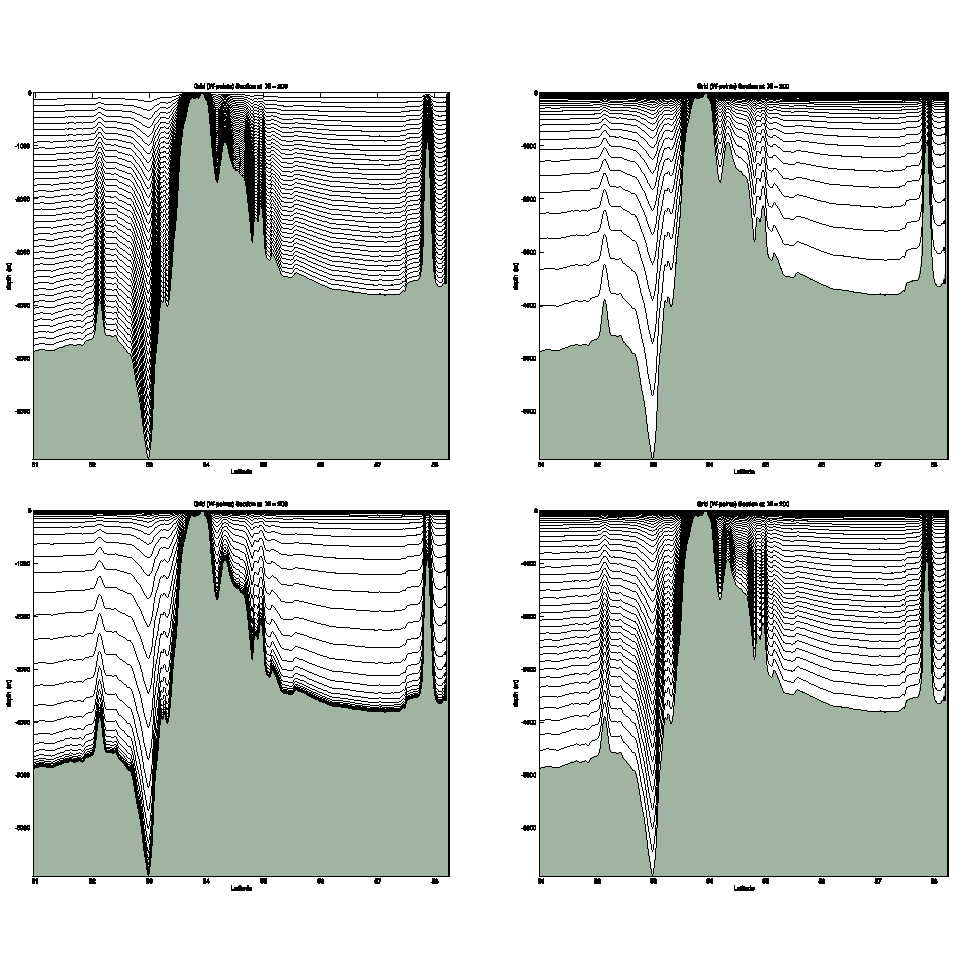
\includegraphics{pics/scoord}
\end{picture}

\caption{The $\sigma$-surfaces for the North Atlantic with (a) $\theta =
0.0001$ and $b = 0$, (b) $\theta = 8$ and $b = 0$, (c) $\theta = 8$
and $b = 1$.  (d) The actual values used in this domain were
$\theta = 5$ and $b = 0.4$.}
\label{fscd}
\end{figure}

We find it convenient to define:
\begin{equation}
   H_z \equiv {\partial z \over \partial \sigma} = (\zeta + h) +
   (h - h_c) {\partial C(\sigma) \over \partial \sigma} .
\end{equation}
The derivative of $C(\sigma)$ can be computed analytically:
\begin{equation}
   {\partial C(\sigma) \over \partial \sigma} = (1-b) {\cosh (\theta
   \sigma) \over
   \sinh \theta} \theta + b {\coth ( {1 \over 2} \theta) \over
   2 \cosh^2 [ \theta (\sigma + {1\over 2})] } \theta .
\end{equation}
However, we choose to compute $H_z$ discretely as $\Delta z/ \Delta
\sigma$ since this leads to the vertical sum of $H_z$ being exactly the
total water depth $D$.

Note that though we have used this form of $\sigma$-coordinate, ROMS
is written in such a way as to work with a variety of vertical
mappings. There is one feature which is critical, however. If the free
surface is at rest, $\zeta = 0$, you get one solution for the level
depths $z^{(0)}(k)$. In the case of nonzero $\zeta$, the
displacements must be proportional to $\zeta$ and to the original
distance from the bottom:
\begin{equation}
   z(k) =  z^{(0)} (k) + \zeta \left( 1 + {z^{(0)} (k) \over h}
   \right)
\end{equation}
or
\begin{equation}
   \Delta z(k) = \Delta z^{(0)} (k) \left( 1 + {\zeta \over h}
   \right)
\end{equation}
This ensures that the vertical mass fluxes generated by a purely
barotropic motion will vanish at every interface.

\section{Horizontal curvilinear coordinates}
\label{Curve}
The requirement for a boundary-following coordinate system and for a
laterally variable grid resolution can both be met (for suitably
smooth domains) by introducing an appropriate orthogonal coordinate
transformation in the horizontal.  Let the new coordinates be
$\xi(x,y)$ and $\eta(x,y)$ where the relationship of horizontal arc
length to the differential distance is given by:
\begin{equation}
   (ds)_{\xi} = \left( {1 \over m} \right) d \xi
\end{equation}
\begin{equation}
   (ds)_{\eta} = \left( {1 \over n} \right) d \eta
\end{equation}
Here, $m(\xi,\eta)$ and $n(\xi,\eta)$ are the scale factors which
relate the differential distances $(\Delta \xi,\Delta \eta)$ to the
actual (physical) arc lengths.

It is helpful to write the equations in vector notation and to use
the formulas for div, grad, and curl in curvilinear coordinates (see
\cite{Batchelor}, Appendix 2):
\begin{equation}
   \nabla \phi = \hat{\xi} m {\partial \phi \over \partial \xi} +
                 \hat{\eta} n {\partial \phi \over \partial \eta}
\end{equation}
\begin{equation}
   \nabla \cdot \vec{a} = mn \left[
   {\partial \over \partial \xi} \!\! \left( {a \over n} \right) +
   {\partial \over \partial \eta} \!\! \left( {b \over m} \right)
   \right]
\end{equation}
\begin{equation}
   \nabla \times \vec{a} = mn \left| \begin{array}{ccc}
   \vspace{1 mm}
   {\hat{\xi}_1 \over m} & {\hat{\xi}_2 \over n} & \hat{k} \\
   \vspace{1 mm}
   {\partial \over \partial \xi} &
   {\partial \over \partial \eta} &
   {\partial \over \partial z} \\
   {a \over m} & {b \over n} & c
   \end{array} \right|
\end{equation}
\begin{equation}
   \nabla^2 \phi = \nabla \cdot \nabla \phi = mn \left[ 
   {\partial \over \partial \xi} \!\! \left( {m \over n} 
   {\partial \phi \over \partial \xi} \right) +
   {\partial \over \partial \eta} \!\! \left( {n \over m} 
   {\partial \phi \over \partial \eta} \right) \right]
\end{equation}
where $\phi$ is a scalar and $\vec{a}$ is a vector with components
$a$, $b$, and $c$.

\section{Viscosity and Diffusion}
\label{Nu}

\subsection{Horizontal viscosity}
The horizontal viscosity and diffusion coefficients are scalars which
are read in from \code{ocean.in}.  Several
factors to consider when choosing these values are:
\begin{klist}
   \kitem{spindown time}  The spindown time on wavenumber $k$ is ${1
   \over k^2 \nu_2}$ for the Laplacian operator and ${1 \over k^4
   \nu_4}$ for the biharmonic operator.  The smallest wavenumber
   corresponds to the length $2 \Delta x$ and is $k = {\pi \over
   \Delta x}$, leading to
\begin{equation}
    \Delta t < t_{damp} = {\Delta x^2 \over \pi^2 \nu_2}
    \mbox{\quad or \quad} {\Delta x^4 \over \pi^4 \nu_4}
\end{equation}
This time should be short enough to damp out the numerical noise
which is being generated but long enough on the larger scales to
retain the features you are interested in.  This time should also be
resolved by the model timestep.
   \kitem{boundary layer thickness} The western boundary layer has a
   thickness proportional to 
\begin{equation}
    \Delta x < L_{BL} = \left( {\nu_2 \over \beta} \right)^{1 \over 3}
    \mbox{\quad and \quad}
    \left( {\nu_4 \over \beta} \right)^{1 \over 5}
\end{equation}
for the Laplacian and biharmonic viscosity, respectively.  We have
found that the model typically requires the boundary layer to be
resolved with at least one grid cell.  This leads to coarse grids
requiring large values of $\nu$.
\end{klist}

\subsection{Horizontal Diffusion}
We have chosen anything from zero to the value of the horizontal
viscosity for the horizontal diffusion coefficient.  One common choice
is an order of magnitude smaller than the viscosity.

\subsection{Vertical Viscosity and Diffusion}
ROMS stores the vertical mixing coefficients in arrays with three
spatial dimensions called
\code{Akv} and \code{Akt}.  \code{Akt} also has a fourth dimension
specifying which tracer, so
that temperature and salt can have differing values.  Both \code{Akt}
and \code{Akv} are stored at $w$-points in the model;
horizontal averaging is done to obtain \code{Akv} at the horizontal $u$
and $v$-points.  The values for these coefficients can be set in a
number of ways, as described in \S\ref{Vmix}.

\section{Radiant heat fluxes}
\label{shortwave}

As was seen in \S\ref{Growth}, the model thermodynamics requires
fluxes of latent and sensible heat and longwave and shortwave
radiation.  We follow the lead of
\citet{Parkinson} in computing these terms.

\subsection{Shortwave radiation}

The Zillman equation for radiation under cloudless skies is:
\begin{equation}
   Q_o = {S \cos^2 Z \over (\cos Z + 2.7) e \times 10^{-5} + 1.085
   \cos Z + 0.10}
\end{equation}
where the variables are as in Table \ref{radvars}.  The cosine of the
zenith angle is computed using the formula:
\begin{equation}
   \cos Z = \sin \phi \sin \delta + \cos \phi \cos \delta \cos H\!A .
\end{equation}
The declination is 
\begin{equation}
   \delta = 23.44^{\circ} \times \cos \left[ (172 - {\rm day \, of \, year})
   \times 2 \pi / 365 \right]
\end{equation}
and the hour angle is
\begin{equation}
   H\!A = (12 \, {\rm hours - solar \, time}) \times \pi / 12 .
\end{equation}
The correction for cloudiness is given by
\begin{equation}
   SW\!\!\downarrow = Q_o ( 1 - 0.6 c^3) .
\end{equation}
%An estimate of the cloud fraction $c$ will be provided by Jennifer
%Francis \citep{Francis00}.

\begin{table}[t]
\hspace{11 mm}
\vbox{
\begin{tabular}{|c|c|l|} \hline
Variable & Value & Description \\ \hline

$(a,b)$ & (9.5, 7.66) & vapor pressure constants over ice \\
$(a,b)$ & (7.5, 35.86) & vapor pressure constants over water \\
$c$ && cloud cover fraction \\
$C_E$ & $1.75 \times 10^{-3}$ & transfer coefficient for latent heat \\
$C_H$ & $1.75 \times 10^{-3}$ & transfer coefficient for sensible heat\\
$c_p$ & 1004 J kg$^{-1}$ K$^{-1}$ & specific heat of dry air \\
$\delta$ && declination \\
$e$ && vapor pressure in pascals \\
$e_s$ && saturation vapor pressure \\
$\epsilon$ & 0.622 & ratio of molecular weight of water to dry air \\
$H\!A$ && hour angle \\
$L$ & $2.5 \times 10^6$ J kg$^{-1}$ & latent heat of vaporization \\
$L$ & $2.834 \times 10^6$ J kg$^{-1}$ & latent heat of sublimation \\
$\phi$ && latitude \\
$Q_o$ && incoming radiation for cloudless skies \\
$q_s$ && surface specific humidity \\
$q_{10 \rm m}$ && 10 meter specific humidity \\
$\rho_a$ && air density \\
$S$ & 1353 W m$^{-2}$ & solar constant \\
$\sigma$ & $5.67 \times 10^{-8}$ W m$^{-2}$ K$^{-4}$ &
Stefan-Boltzmann constant \\
$T_a$ && air temperature \\
$T_d$ && dew point temperature \\
$T_{s\!f\!c}$ && surface temperature of the water/ice/snow \\
$V_{wg}$ && geostrophic wind speed \\
$Z$ && solar zenith angle \\

\hline
\end{tabular}
}
\caption{Variables used in computing the incoming radiation and latent
and sensible heat}
\label{radvars}
\end{table}

\subsection{Longwave radiation}

The clear sky formula for incoming longwave radiation is given by:
\begin{equation}
   F\!\downarrow\, = \sigma T_a^4 \left\{1 - 0.261 \exp \left[ -7.77 \times 10^{-4}
   (273 - T_a) ^2 \right] \right\}
\end{equation}
while the cloud correction is given by:
\begin{equation}
   LW\!\downarrow\, = (1 + 0.275 c)\, F\!\downarrow .
\end{equation}

\subsection{Sensible heat}

The sensible heat is given by the standard aerodynamic formula:
\begin{equation}
   H\!\downarrow\, = \rho_a c_p C_H V_{wg} (T_a - T_{s\!f\!c}) .
\end{equation}

\subsection{Latent heat}

The latent heat depends on the vapor pressure and the saturation vapor
pressure given by:
\begin{eqnarray}
   e & = & 611 \times 10^{a(T_d - 273.16) / (T_d - b)} \\
   e_s & = & 611 \times 10^{a(T_{s\!f\!c} - 273.16) / (T_{s\!f\!c} - b)}
\end{eqnarray}
The vapor pressures are used to compute specific humidities according
to:
\begin{eqnarray}
   q_{10 \rm m} & = & {\epsilon e \over p - (1 - \epsilon) e} \\
   q_s & = & {\epsilon e_s \over p - (1 - \epsilon) e_s}
\end{eqnarray}
The latent heat is also given by a standard aerodynamic formula:
\begin{equation}
   LE\!\downarrow\, = \rho_a L C_E V_{wg} (q_{10 \rm m} - q_s) .
\end{equation}
Note that these need to be computed independently for the ice-covered
and ice-free portions of each gridbox since the empirical factors
$a$ and $b$ and the factor $L$ differ depending on the surface type.

\section{The C preprocessor}
\label{Cpp}

The C preprocessor, \code{cpp}, is a standalone program which comes
with most C compilers. On older UNIX systems it was not in the default
path, but in \code{/lib} or in \code{/usr/lib}. Most modern systems
have some version of \code{gcc} which comes with a quite capable
\code{cpp}. Just be sure to give it the \code{-traditional} flag.

This Appendix describes the C preprocessor as used in ROMS with the
Fortran language.  A more complete description is given by
\cite{K&R}.  More practical advice on using
\code{cpp} is given by \cite{Hazard}.

\subsection{File inclusion}
Placing common blocks in smaller files, which are then included in each
subroutine, is the easiest way to make sure that the common blocks are
declared consistently.  Many Fortran compilers support an include
statement where the compiler replaces the line
\begin{verbatim}
            include 'file.h'
\end{verbatim}
with the contents of \code{file.h}; \code{file.h} is assumed
to be in the current directory.  The C preprocessor has an equivalent
include statement:
\begin{verbatim}
      #include "file.h"
\end{verbatim}
We are using the C preprocessor style of include because many of the
ROMS include files are not pure Fortran and must be processed by
\code{cpp}.

\subsection{Macro substitution}
A macro definition has the form
\begin{verbatim}
      #define    name           replacement text
\end{verbatim}
where ``name'' would be replaced with ``replacement text''
throughout the rest of the file.  This was used in SCRUM as a
reasonably portable way to get 64-bit precision:
\begin{verbatim}
      #define  BIGREAL     real*8
\end{verbatim}
It is customary to use uppercase for \code{cpp} macros---the C
preprocessor is case sensitive.

It is also possible to define macros with arguments, as in
\begin{verbatim}
      #define av2(a1,a2)        (.5 * ((a1) + (a2)))
\end{verbatim}
although this is riskier than the equivalent statement function
\begin{verbatim}
            av2(a1,a2) = .5 * (a1 + a2)
\end{verbatim}
The statement function is preferable because it allows the compiler
to do type checking and because you don't have to be as careful
about using enough parentheses.

The third form of macro has no replacement text at all:
\begin{verbatim}
      #define  MASKING
\end{verbatim}
In this case, \code{MASKING} will evaluate to \code{true} in the
conditional tests described below.

\subsection{Conditional inclusion}
It is possible to control which parts of the code are seen by the
Fortran compiler by the use of \code{cpp}'s conditional inclusion.
For example, the statements
\begin{verbatim}
      #ifdef MASKING
      # include "mask.h"
      #endif /* MASKING */
              :
      # ifdef MASKING
      c
      c  Apply Land/Sea mask: slipperiness.
      c
            do j=1,M
              do i=2,Lm
                Uflux(i,j)=Uflux(i,j)*pmask(i,j)
              enddo
            enddo
      # endif /* MASKING */
\end{verbatim}
will not be in the Fortran source code if \code{MASKING} has not
been defined.  Likewise,
\code{\#ifndef} tests for a macro being undefined:
\begin{verbatim}
      #ifndef RMDOCINC
      c  rmask       Mask at RHO-points (0=Land, 1=Sea).
      c  pmask       Slipperiness mask at PSI-points (0=Land, 1=Sea,
      c                                               1-gamma2=boundary).
      c  umask       Mask at U-points (0=Land, 1=Sea).
      c  vmask       Mask at V-points (0=Land, 1=Sea).
      c
      c=======================================================================
      #endif
\end{verbatim}

There are also \code{\#else} and \code{\#elif} (else if) statements.
%although \code{\#elif} is newer and is not supported by all versions of
%\code{cpp}.
An example using \code{\#else} and \code{\#elif} is
shown:
\begin{verbatim}
#ifdef SOLITON
        real(r8) :: g = 1.0_r8                  ! non-dimensional
# elif defined WBC_1 || defined WBC_2 || defined WBC_3
        real(r8) :: g = 9.8_r8                  ! m/s2
# elif defined CIRCLE
        real(r8) :: g = 3.92e-2_r8                  ! m/s2
#else
        real(r8) :: g = 9.81_r8                 ! m/s2
#endif
\end{verbatim}

Actually, \code{\#ifdef} is a restricted version of the more general
test
\begin{verbatim}
      #if     expression
\end{verbatim}
where ``expression'' is a constant integer value.  Zero evaluates
to \code{false} and everything else is considered \code{true}.
Compound expressions may be built using the C logical operators:
\begin{verbatim}
        &&           logical and
        ||           logical or
        !            logical not
\end{verbatim}
These symbols would be used as in the following example:
\begin{verbatim}
      #if defined CANYON_A || defined CANYON_B
            do j=0,M
              do i=0,L
                yc=c32000-c16000*(sin(pi*xr(i,j)/xl))**24
                h(i,j)=c20+p5*(hmax-c20)*(c1+tanh((yr(i,j)-yc)/c10000))
              enddo
            enddo
      #endif
\end{verbatim}

\subsection{C comments}
The C preprocessor will also delete C language comments starting
with \code{/*} and ending with \code{*/} as in:
\begin{verbatim}
       #endif  /* MASKING */
\end{verbatim}
When mixed with Fortran code, it is safer to use a Fortran
comment.

\subsection{A note on style}
In ROMS, the style adopted is as shown above and here:
\begin{verbatim}
#define NEP5
#if defined NEP5 || defined BERING
        :
# ifdef MASKING
        :
# endif
#endif
\end{verbatim}
The \code{gnu} community has instead adopted this style:
\begin{verbatim}
#define NEP5  1
#if NEP5 || BERING
        :
# if MASKING
        :
# endif
#endif
\end{verbatim}
Both styles work and you should be aware that there's more than one
way to do it.

\subsection{Potential problems}
The use of the C preprocessor is not entirely free of problems, but
many can be worked around or avoided by using the \code{gnu} version of
\code{cpp} with the \code{-traditional} flag.
   \begin{enumerate}
     \item Apostrophes in Fortran comments.  \code{cpp} does not
     know that it is in a comment and some versions will complain about
     unmatched apostrophes in the following:
     \begin{verbatim}
  !  Some useful comment about Green's functions.
     \end{verbatim}
     \item \CC\ comments.  Some of the newer versions of
     \code{cpp} will remove \CC\ comments which go from '//' to
     the end of the line.  Some perfectly reasonable Fortran lines
     contain two consecutive slashes, such as:
     \begin{verbatim}
        common // var1, var2
    44  format(//)
     \end{verbatim}
     and Fortran 90 string concatenation:
     \begin{verbatim}
        mystring = 'Hello, ' // 'World!'
     \end{verbatim}
     \item Macro replacement.  One feature of \code{cpp} is that you
     can define macros and have it perform replacements.  The code:
     \begin{verbatim}
  #define REAL double precision
        REAL really_long_variable, second_long_variable
     \end{verbatim}
     becomes
     \begin{verbatim}
        double precision really_long_variable, second_long_variable
     \end{verbatim}
     and you run the risk of creating lines which are longer than 72
     characters in length.

     Also, make sure that your macros will not be found anywhere else
     in the code.  I used to use \code{\#define DOUBLE} for double
     precision until it was pointed out to me that \code{DOUBLE}
     \code{PRECISION} is perfectly valid Fortran.  Since a string
     that is simply ``defined'' becomes 1, the macro processor would
     turn this into \code{1 PRECISION}.
  \end{enumerate}

\subsection{Modern Fortran}
I started working on these ocean models before 1990, much less before
Fortran 90 compilers were generally available.  Fortran 90's \code{kind}
feature as used in ROMS is a better way to handle the \code{BIGREAL}
type declarations.  On the other hand, Fortran 90 does not include
conditional compilation.  However, it is deemed useful enough that the
Fortran 2003 standard has the coco means of conditional compilation.
We {\em might} start using this in about ten years.

%\section{The \code{patch} program}
\label{Patch}
We sometimes discover things in SCRUM which we would like to modify,
either to fix bugs, or to add new features.
Hernan Arango keeps track of these changes
and periodically sends patches to the
list of known SCRUM users so that they can update their versions.  By
sending out these changes rather than the whole updated model, people
can acquire bug fixes and still retain the changes they have made to
SCRUM for their own applications.

Larry Wall has written a program to take the output of \code{diff} and
automatically apply it to the old version of a file to create the new
version.  This program is called \code{patch} and is available from all
the \code{gnu} archive sites.  If the output of \code{diff} has been
saved in the file \code{scrum.patch.20} then \code{patch} would be used
as follows:
\begin{verbatim}
        patch < scrum.patch.20
\end{verbatim}
As \code{patch} updates the files, it leaves the original of
\code{file} in \code{file.orig}.  If it gets confused for some reason
(if you modified the lines of code \code{patch} wants to change)
it will create a \code{file.rej} file.  I
often check to see if any \code{.rej} files get created---these can be
used to patch \code{file} by hand and can then be deleted.

%\newpage
%\mbox{}
\section{Building ROMS}
\label{Build}

\subsection{Environment Variables for \code{make}}
\label{make_var}

ROMS has a growing list of choices the user must make about the
compilation before starting the compile process,
set in user-defined variables. Since we now use \code{gnu make}, it is
possible to set the value of these variables in the Unix environment,
rather than necessarily inside the \code{Makefile} (see \S\ref{Gmake}).
The user-definable variables understood by the ROMS \code{makefile} are:
\begin{klist}

\kitem{ROMS\_APPLICATION} Set the \code{cpp} option defining the particular
application. This is used for setting up options inside the code
specific to this application and also determines the name of the
\code{.h} header file for it. This can be either a predefined
case, such as \code{BENCHMARK}, or one of your own, such as \code{NEP5}.

\kitem{MY\_HEADER\_DIR} Sets the path to the user's header file, if
any. It can be left empty for the standard cases, where \code{benchmark.h}
and the like are found in \code{ROMS/Include}, which is already in
the search path. In the case of \code{NEP5}, this is set to
\code{Apps/NEP} where \code{nep5.h} resides.

\kitem{MY\_ANALYTICAL\_DIR} Sets the path to the user's analytic files
described in \S\ref{Functionals}, if any. This can be \code{User/Functionals}
or some other location. I tend to place both the header file and the
functionals in the same directory, one directory per application.

\kitem{MY\_CPP\_FLAGS} Set tunable \code{cpp} options. Sometimes it is desirable
to activate one or more \code{cpp} options to run different variants of the
same application without modifying its header file. If this is the
case, specify each option here using the \code{-D} syntax. Notice that
you need to use the shell's quoting syntax (either single or double
quotes) to enclose the definition if you are using one of the build
scripts below.

\kitem{NestedGrids} Integer number of grids in the setup, usually 1.

\kitem{Compiler-specific Options} These flags are used by the files
inside the \code{Compilers} directory.
\begin{klist}
  \kitem{USE\_DEBUG} Set this to \code{on} to turn off optimization
and turn on the \code{-g} flag for debugging.

  \kitem{USE\_MPI} Set this if running an MPI parallel job.
  \kitem{USE\_OpenMP} Set this if running an OpenMP parallel job.
  \kitem{USE\_MPIF90} I'm frankly not sure about this one. I suppose
  if you have both mpich and some other MPI for a given
  compiler/system pair, this could be used to switch between them.
  \kitem{USE\_LARGE}  Some systems support both 32-bit and 64-bit
  options. Select this to get 64-bit addressing, usually used for
  programs need more than 2 GB of memory.
  \kitem{NETCDF\_INCDIR} The location of the \code{netcdf.mod} and
  \code{typesizes.mod} files.
  \kitem{NETCDF\_LIBDIR} The location of the NetCDF library.
  \kitem{USE\_NETCDF4} Set this if linking against the NetCDF4
  library, which needs the HDF5 library and therefore:
  \kitem{HDF5\_LIBDIR} The location of the HDF5 library.
\end{klist}

\kitem{FORT} A shorthand name for the compiler to be used when
selecting which system-compiler file is to be included from the
\code{Compilers} directory. See section \S\ref{Inc_fort} and
\S\ref{make_env}.

\kitem{Local File Options}
\begin{klist}
  \kitem{BINDIR} Directory in which to place the binary executable.
The default is ``\code{.}'', the current (top) directory.

  \kitem{SCRATCH\_DIR} Put the \code{.f90} and the temporary binary files
in a build directory to avoid clutter. The default is \code{Build}
under the top directory. It can also point to differing places if you want
to keep these files for multiple projects at the same time, each in
their own directory.
\end{klist}
\end{klist}

\subsection{Providing the Environment}
\label{make_env}

Before compiling, you will need to find out some background information:
\begin{itemize}
 \item What is the name of your compiler?
 \item What is returned by \code{uname -s} on your system?
 \item Is there a working NetCDF library?
 \item Where is it?
 \item Was it built with the above compiler?
 \item Do you have access to MPI or OpenMP?
\end{itemize}
As described more fully in \S\ref{Inc_fort}, the \code{makefile} will be
looking for a file in the \code{Compilers} directory with the
combination of your operating system and your compiler. For
instance, using Linux and the Pathscale compiler, the file would be
called \code{Linux-path.mk}. Is the corresponding file for your
system and compiler in the \code{Compilers} directory? If not, you
will have to create it following the existing examples there.

Next, there are two ways to provide the location for the NetCDF
files (and optional HDF5 library). One is by editing the corresponding
lines in your system-compiler file. Another way is through the
Unix environment variables. If you are always going to be using
the same compiler on each system, you can edit your \code{.profile}
or \code{.login} files to globally set them. Here is an example for
\code{tcsh}:
\begin{verbatim}
setenv NETCDF_INCDIR /usr/local/netcdf4/include
setenv NETCDF_LIBDIR /usr/local/netcdf4/lib
setenv HDF5_LIBDIR /usr/local/hdf5/lib
\end{verbatim}
The \code{ksh/bash} equivalent is:
\begin{verbatim}
export NETCDF_INCDIR=/usr/local/netcdf4/include
export NETCDF_LIBDIR=/usr/local/netcdf4/lib
export HDF5_LIBDIR=/usr/local/hdf5/lib
\end{verbatim}

\subsubsection{Build scripts}

If you have more than one application (or more than one compiler),
you will get tired of editing the \code{makefile}.
One option is to have a \code{makefile} for each configuration, then
type:
\begin{verbatim}
    make -f makefile.circle_pgi
\end{verbatim}
for instance. Another option of keeping track of the user-defined
choices in a \code{build script}. The advantage is that updates
to the \code{build scripts} are less frequent than updates to the
\code{makefile}. There are now two of these scripts in the \code{ROMS/Bin}
directory: \code{build.sh} (which is surprisingly a \code{csh} script)
and \code{build.bash}.  The \code{build scripts} use environment variables
to provide values for the list above, overwriting those found in the ROMS
\code{makefile}. Just as in the multiple \code{makefile} option, you will
need as many copies of the build script as you have applications. The
scope of these variables is local to the build script, allowing you to
compile different applications at the same time from the same sources
as long as each \code{\$(SCRATCH\_DIR)} is unique.

Both scripts have the same options:
\begin{klist}
  \kitem{-j \code{[N]}} Compile in parallel using \code{N} cpus,
  omit argument for all available CPUs.
  \kitem{-noclean}    Do not clean already compiled objects.
\end{klist}
Note that the default is to compile serially and to issue a
``\code{make clean}'' before compiling. It is left as an exercise
for the user if they prefer different default behavior.

There are also a few variables which are not recognized by the ROMS
\code{makefile}, but are used locally inside the build script. These
are:
\begin{klist}
\kitem{MY\_PROJECT\_DIR} This is used in setting
\code{\$(SCRATCH\_DIR)} and \code{\$(BINDIR)}.

\kitem{MY\_ROMS\_SRC} Set the path to the user's local current ROMS source
code. This is used so that the script can be run from any directory,
not necessarily only from the top ROMS directory.
\end{klist}

\section{\code{Makefiles}}
\label{Gmake}
One of the software development tools which comes with the UNIX
operating system is called \code{make}. \code{Make} has many uses,
but is most commonly used to keep track of how a large program
should be compiled. ROMS now requires the \code{gnu} version of 
\code{make}, sometimes known as \code{gmake} (Mecklenburg \cite{GMAKE}).
This appendix describes generic \code{make}, the \code{gnu}
enhancements to \code{make}, as well as describing the
\code{makefile} structure used in ROMS. This material first
appeared in the \href{http://www.arsc.edu/support/news/HPCnews.shtml}{ARSC
HPC Newsletter} in several segments and has been updated and restructured
here.

\subsection{Introduction to Portable \code{make}}

\code{Make} gets its instructions from a description file, by default named
\code{makefile} or \code{Makefile}. This file is called the
\code{Makefile}, but other files
can be used by invoking \code{make} with the \code{-f} option:
\begin{verbatim}
     make -f Makefile.yukon
\end{verbatim}

The ancester to ROMS originally had a \code{Makefile} that looked
something like:
\begin{verbatim}
model: main.o init.o plot.o
<TAB>   f77 -o model main.o init.o plot.o

main.o: main.f
<TAB>   f77 -c -O main.f

init.o: init.f
<TAB>   f77 -c -O init.f

plot.o: plot.f
<TAB>   f77 -c -O0 plot.f

clean:
<TAB>   rm *.o core
\end{verbatim}
The default thing to build is \code{model}, the first target. The syntax
is:
\begin{verbatim}
target: dependencies
<TAB>  command
<TAB>  command
\end{verbatim}
The target \code{model} depends on the object files, \code{main.o}
and friends. They have to exist and be up to date before model's link
command can be run. If the target is out of date according to the
timestamp on the file, then the commands will
be run. Note that the tab is required on the command lines.

The other targets tell \code{make} how to create the object files
and that they in turn have dependencies.  To compile \code{model}, simply
type ``\code{make}''. \code{Make} will look for the file \code{makefile},
read it, and do whatever is necessary to make \code{model} up
to date. If you edit \code{init.f}, that file will be newer than
\code{init.o}. \code{Make} would see that \code{init.o} is out of date
and run the ``\code{f77 -c -O init.f}'' command. Now \code{init.o}
is newer than \code{model}, so the link command ``\code{f77 -o model
main.o init.o plot.o}'' must be executed.

To clean up, type ``\code{make clean}'' and the \code{clean} target will
be brought up to date. The \code{clean} target has no dependencies. What
happens in that case is that the command (``\code{rm *.o core}'') will
always be executed.

The original version of this \code{Makefile} turned off
optimization on \code{plot.f} due to a compiler bug, but hopefully you
won't ever have to worry about that.

\subsubsection{Macros}

\code{Make} supports a simple string substitution macro. Set it with:
\begin{verbatim}
MY_MACRO = nothing today
\end{verbatim}
and refer to it with:
\begin{verbatim}
$(MY_MACRO)
\end{verbatim}

The convention is to put the macros near the top of your \code{Makefile}
and to use upper case. Also, use separate macros for the name of
your compiler and the flags it needs:
\begin{verbatim}
F90 = f90
F90FLAGS = -O3
LIBDIR = /usr/local/lib
LIBS = -L$(LIBDIR) -lmylib
\end{verbatim}

Let's rewrite our \code{Makefile} using macros:
\begin{verbatim}
#
# IBM version
#
F90 = xlf90_r
F90FLAGS = -O3 -qstrict
LDFLAGS = -bmaxdata:0x40000000

model: main.o init.o plot.o
        $(F90) $(LDFLAGS) -o model main.o init.o plot.o

main.o: main.f
        $(F90) -c $(F90FLAGS) main.f

init.o: init.f
        $(F90) -c $(F90FLAGS) init.f

plot.o: plot.f
        $(F90) -c $(F90FLAGS) plot.f

clean:
        rm *.o core
\end{verbatim}

Now when we change computers, we only have to change the compiler name
in one place. Likewise, if we want to try a different optimization level,
we only specify that in one place.

Notice that you can use comments by starting the line with a \code{\#}.

\subsubsection{Implicit Rules}

\code{Make} has some rules already built in. For fortran, you might be able
to get away with:
\begin{verbatim}
OBJS = main.o init.o plot.o

model: $(OBJS)
        $(FC) $(LDFLAGS) -o model $(OBJS)
\end{verbatim}
as your whole \code{Makefile}. \code{Make} will automatically invoke its
default Fortran compiler, possibly \code{f77} or \code{g77}, with whatever
default compile options it happens to have (\code{FFLAGS}). One built
in rule often looks like:
\begin{verbatim}
.c.o:
        $(CC) $(CFLAGS) -c $<
\end{verbatim}
which says to compile \code{.c} files to \code{.o} files using the
compiler \code{CC} and options \code{CFLAGS}. We can write our own suffix
rules in this same style.  The only thing to watch for is that make by
default has a limited set of file extentions that it knows about. Let's
write our \code{Makefile} using a suffix rule:
\begin{verbatim}
#
# Cray version
#
F90 = f90
F90FLAGS = -O3
LDFLAGS =

.f.o:
        $(F90) $(F90FLAGS) -c $<

model: main.o init.o plot.o
        $(F90) $(LDFLAGS) -o model main.o init.o plot.o

clean:
        rm *.o core
\end{verbatim}

\subsubsection{Dependencies}

There may be additional dependencies beyond the \code{source->object} ones.
In our little example, all our source files include a file called
\code{commons.h}. If \code{commons.h} gets modified to add a new variable,
everything must be recompiled. \code{Make} won't know that unless you
tell it:
\begin{verbatim}
# include dependencies
main.o: commons.h
init.o: commons.h
plot.o: commons.h
\end{verbatim}
Fortran 90 introduces module dependencies as well. See \S\ref{sfm}
for how we automatically generate this dependency information.

The most common newbie mistake is to forget that the commands after
a target {\em have} to start with a tab.

\subsection{\code{gnu make}}

Over the years, the community has moved from the stance of writing
portable \code{Makefiles} to a stance of just using a powerful, portable
\code{make}. The previous section described a portable subset of
\code{make} features. We now delve into some of the more powerful
tools available in \code{gnu make}.

\subsubsection{Make rules}

The core of \code{make} hasn't changed in decades, but concentrating on
\code{gmake} allows one to make use of its nifty little extras designed
by real programmers to help with real projects. The first change that
matters to my \code{Makefiles} is the change from suffix rules to
pattern rules. I've always found the \code{.SUFFIXES} list to be odd,
especially since \code{.f90} is not in the default list. Good riddance
to all of that! For a concrete example, the old way to provide a rule
for going from \code{file.f90} to \code{file.o} is:
\begin{verbatim}
.SUFFIXES: .o .f90 .F .F90
.f90.o:
<TAB>   $(FC) -c $(FFLAGS) $<
\end{verbatim}
while the new way is:
\begin{verbatim}
%.o: %.f90
<TAB>   $(FC) -c $(FFLAGS) $<
\end{verbatim}
In fact, going to a uniform \code{make} means that we can figure out what
symbols are defined and use their standard values---in this case,
\$\code{(FC)} and \$\code{(FFLAGS)} are the built-in default names
for the compiler and its options.
If you have any
questions about this, you can always run \code{make} with the \code{-p} (or
\code{-\mbox{}-print-data-base}) option. This prints out all the rules
\code{make} knows about, such as:
\begin{verbatim}
# default
COMPILE.f = $(FC) $(FFLAGS) $(TARGET_ARCH) -c
\end{verbatim}
Printing the rules database will show variables that \code{make} is
picking up from the environment, from the \code{Makefile}, and from its
built-in rules---and which of these sources is providing each
value.

\subsubsection{Assignments}

In the old days, I only used one kind of assignment: \code{=} (equals
sign). \code{Gmake} has several kinds of assignment (other \code{makes}
might as well, but I no longer have to know or care). An example of
the power of \code{gnu make} is shown by an example from my Cray X1
\code{Makefile}.  There is a routine which runs much more quickly if a
short function in another file is inlined. The way to accomplish this is
through the \code{-O inlinefrom=file} directive to the compiler. I can't
add this option to \code{FFLAGS}, since the inlined routine won't compile
with this directive---there is only the one file that needs it. I had:
\begin{verbatim}
    FFLAGS = -O 3,aggress -e I -e m
    FFLAGS2 = -O 3,aggress -O inlinefrom=lmd_wscale.f90 -e I -e m

lmd_skpp.o:
<TAB>   $(FC) -c $(FFLAGS2) $*.f90
\end{verbatim}
The first change I can make to this using other assignments is:
\begin{verbatim}
    FFLAGS := -O 3,aggress -e I -e m
    FFLAGS2 := $(FFLAGS) -O inlinefrom=lmd_wscale.f90
\end{verbatim}
The \code{:=} assignment means to evaluate the right hand side immediately.
In this case, there is no reason not to, as long as the second
assigment follows the first one (since it's using the value of
\$\code{(FFLAGS))}. For the plain equals, \code{make} doesn't evaluate the
right-hand side until its second pass through the \code{Makefile}. However,
\code{gnu make}
supports an assignment which avoids the need for \code{FFLAGS2} entirely:
\begin{verbatim}
lmd_skpp.o: FFLAGS += -O inlinefrom=lmd_wscale.f90
\end{verbatim}
What this means is that for the target \code{lmd\_skpp.o} only, append the
inlining directive to \code{FFLAGS}. I think this is pretty cool!

One last kind of assignment is to set the value only if there is no
value from somewhere else (the environment, for instance):
\begin{verbatim}
     FC ?= mpxlf90_r
\end{verbatim}
If we used \code{:=} or \code{=}, we would override the value from the
environment.

\subsubsection{Include and a Few Functions}
\label{Inc_fort}

One reasonably portable \code{make} feature is the include directive. It
can be used to clean up the \code{Makefile} by putting bits in an
include file. The syntax is simply:
\begin{verbatim}
   include file
\end{verbatim}
and we use it liberally to keep the project
information neat. We can also include a file with the system/compiler
information in it, assuming we have some way of deciding {\em which}
file to include. We can use \code{uname -s} to find out which operating
system we're using. We also need to know which compiler we're using.

One user-defined variable is called \code{FORT}, the name of the
Fortran compiler. This value is combined with the result of
``\code{uname -s}'' to
provide a machine and compiler combination. For instance, \code{ftn} on
Linux is the Cray cross-compiler. This would link to a different copy
of the NetCDF library and use different compiler flags than the Intel
compiler which might be on the same system.
\begin{verbatim}
# The user sets FORT:
  FORT ?= ftn
  OS := $(shell uname -s | sed 's/[\/ ]/-/g')

  include $(COMPILERS)/$(OS)-$(strip $(FORT)).mk
\end{verbatim}
We pick one include file at compile time, here picking
\code{Linux-ftn.mk}, containing the Cray cross-compiler information. The
value \code{Linux} comes from the \code{uname} command, the \code{ftn}
comes from the user, and the two are concatenated.
The sed command will turn the
slash in \code{UNICOS/mp} into a dash; the native Cray include file is
\code{UNICOS-mp-ftn.mk}. Strip is a built-in function to strip away
any extra white space.

Another tricky system is \code{CYGWIN}, which puts a version number
in the \code{uname} output, such as \code{CYGWIN\_NT-5.1}. \code{Gnu make} has
quite a few built-in functions, one of which allows us to do string
substitution:
\begin{verbatim}
OS := $(patsubst CYGWIN_%,CYGWIN,$(OS))
\end{verbatim}
In \code{make}, the \code{\%} symbol is a sort of wild card, much
like \code{*} in the shell.
Here, we match \code{CYGWIN} followed by an underscore and anything else,
replacing the whole with simply \code{CYGWIN}. Another example of a
built-in function is the substitution we do in:
\begin{verbatim}
   objects = $(subst .F,.o,$(sources))
\end{verbatim}
where we build our list of objects from the list of sources.
There are quite a few other functions, plus the user can define
their own. From the book\cite{GMAKE}:
\begin{quote}
GNU make supports both built-in and user-defined functions.
A function invocation looks much like a variable reference, but
includes one or more parameters separated by commas.  Most built-in
functions expand to some value that is then assigned to a variable
or passed to a subshell. A user-defined function is stored in a
variable or macro and expects one or more parameters to be passed
by the caller.
\end{quote}
We will show some user-defined functions in \S\ref{make_fun2}.

\subsubsection{Conditionals}

We used to have way too many \code{Makefiles}, a separate one for each
of the serial/MPI/OpenMP versions on each system (if supported). For
instance, the name of the IBM compiler changes when using MPI; the
options change for OpenMP. The compiler options also change when using
64-bit addressing or for debugging.
A better way to organize this is to have the user select 64-bit or not, MPI
or not, etc., then use conditionals. The complete list of
user definable \code{make} variables is given in \S\ref{make_var}.

\code{Gnu make} supports two kinds of \code{if} test, \code{ifdef} and
\code{ifeq} (plus the
negative versions \code{ifndef, ifneq}). The example from the book is:
\begin{verbatim}
ifdef COMSPEC
   # We are running Windows
else
   # We are not on Windows
endif
\end{verbatim}
An example from the IBM include file is:
\begin{verbatim}
ifdef USE_DEBUG
           FFLAGS += -g -qfullpath
else
           FFLAGS += -O3 -qstrict
endif
\end{verbatim}
To test for equality, an example is:
\begin{verbatim}
ifeq ($(USE_MPI),on)
   # Do MPI things
endif
\end{verbatim}
or 
\begin{verbatim}
ifeq "$(USE_MPI)" "on"
   # Do MPI things
endif
\end{verbatim}
The user has to set values for the \code{USE\_MPI}, \code{USE\_DEBUG},
and \code{USE\_LARGE} switches in the \code{Makefile} or the build
script {\em before} the compiler-dependent piece is included:
\begin{verbatim}
    USE_MPI ?= on
    USE_DEBUG ?=
    USE_LARGE ?=
\end{verbatim}
The \code{Makefile} uses the conditional assign ``\code{?=}''
in case a build script is used to set them in the environment.
Be sure to leave the switches meant to be off set to an empty string---the
string ``\code{off}'' will test true on an \code{ifdef} test.

\subsection{Multiple Source Directories the ROMS Way}

There's more than one way to divide your sources into separate
directories. The choices we have made include nonrecursive \code{make}
and putting the temporary files in their own \code{\$(SCRATCH\_DIR)}
directory. These include the \code{.f90} files which have been through
the C preprocessor, object files, module files, and libraries.

\subsubsection{Directory Structure}

The directory structure of the source code has the top directory,
a \code{Master} directory, a \code{ROMS} directory with a number of
subdirectories, and several other directories. \code{Master} contains
the main program while the rest contain sources for libraries and
other files. Note that the bulk of the source code gets compiled into
files that become libraries with the \code{ar} command, one library per
directory. There is also a \code{Compilers} directory for the system-
and compiler-specific \code{Makefile} components.

\subsubsection{Conditionally Including Components}

The \code{makefile} will build the lists of libraries to create and source
files to compile. They start out empty at the top of the
\code{makefile}:
\begin{verbatim}
  sources    := 
  libraries  :=
\end{verbatim}
That's simple enough, but the list of directories to search for
these sources will depend on the options chosen by the user, not
just in the \code{make} options (\S\ref{make_var}), but inside the
\code{ROMS\_HEADER} file as well. How does this happen? Once \code{make}
knows how to find the \code{ROMS\_HEADER}, it is used by \code{cpp}
to generate an include file telling \code{make} about these other options.
\begin{verbatim}
MAKE_MACROS := Compilers/make_macros.mk
 MACROS := $(shell cpp -P $(ROMS_CPPFLAGS) Compilers/make_macros.h > \
                 $(MAKE_MACROS); $(CLEAN) $(MAKE_MACROS))
\end{verbatim}
The \code{make\_macros.h} file contains blocks such as:
\begin{verbatim}
#ifdef SWAN_COUPLING
  USE_SWAN := on
#else
  USE_SWAN :=
#endif
\end{verbatim}
The resulting \code{make\_macros.mk} file will simply end up with
either 
\begin{verbatim}
  USE_SWAN := on
\end{verbatim}
or
\begin{verbatim}
  USE_SWAN :=
\end{verbatim}
This file can then be included by the \code{makefile} and the
variable \code{USE\_SWAN} will have the correct state for this
particular compilation. We can now use it and all the similar flags
to build a list of directories.

We initialize two lists:
\begin{verbatim}
 modules  :=
 includes :=    ROMS/Include
\end{verbatim}
Add the adjoint bits:
\begin{verbatim}
ifdef USE_ADJOINT
 modules  +=    ROMS/Adjoint
endif
ifdef USE_ADJOINT
 includes +=    ROMS/Adjoint
endif
\end{verbatim}
Add the bits we'll always need:
\begin{verbatim}
 modules  +=    ROMS/Nonlinear \
                ROMS/Functionals \
                ROMS/Utility \
                ROMS/Modules
 includes +=    ROMS/Nonlinear \
                ROMS/Utility \
                ROMS/Drivers
\end{verbatim}
Then we add in some more:
\begin{verbatim}
ifdef USE_SWAN
 modules  +=    Waves/SWAN/Src
 includes +=    Waves/SWAN/Src
endif

 modules  +=    Master
 includes +=    Master Compilers
\end{verbatim}
Now that our lists are complete, let's put them to use:
\begin{verbatim}
vpath %.F $(modules)
vpath %.h $(includes)
vpath %.f90 $(SCRATCH_DIR)
vpath %.o $(SCRATCH_DIR)

include $(addsuffix /Module.mk,$(modules))

CPPFLAGS += $(patsubst %,-I%,$(includes))
\end{verbatim}
\begin{enumerate}
\item \code{vpath} is a standard \code{make} feature for
providing a list of directories for \code{make} to search for files
of different types. Here we are saying that \code{*.F} files can be
found in the directories provided in the \code{\$(modules)} list, and
so on for the others.

\item For each directory in the \code{\$(modules)} list, \code{make}
will include the file \code{Module.mk} that is found there. More on
these later.

\item For each directory in the \code{\$(includes)} list, add
that directory to the list searched by \code{cpp} with the \code{$-$I}
flag.
\end{enumerate}

\subsubsection{User-defined \code{make} Functions}
\label{make_fun2}

The \code{Module.mk} fragments mentioned before call some
user-defined functions.  It's time to show these functions and
talk about how they work. They get defined in the top Makefile:
\begin{verbatim}
#--------------------------------------------------------------------------
#  Make functions for putting the temporary files in $(SCRATCH_DIR)
#--------------------------------------------------------------------------

# $(call source-dir-to-binary-dir, directory-list)
source-dir-to-binary-dir = $(addprefix $(SCRATCH_DIR)/, $(notdir $1))

# $(call source-to-object, source-file-list)
source-to-object = $(call source-dir-to-binary-dir,   \
                   $(subst .F,.o,$(filter %.F,$1)))

# $(call f90-source, source-file-list)
f90-source = $(call source-dir-to-binary-dir,     \
                   $(subst .F,.f90,$1))

# $(call make-library, library-name, source-file-list)
define make-library
   libraries += $(SCRATCH_DIR)/$1
   sources   += $2

   $(SCRATCH_DIR)/$1: $(call source-dir-to-binary-dir,    \
                      $(subst .F,.o,$2))
       $(AR) $(ARFLAGS) $$@ $$^
       $(RANLIB) $$@
endef

# $(call one-compile-rule, binary-file, f90-file, source-files)
define one-compile-rule
  $1: $2 $3
       cd $$(SCRATCH_DIR); $$(FC) -c $$(FFLAGS) $(notdir $2)

  $2: $3
       $$(CPP) $$(CPPFLAGS) $$(MY_CPP_FLAGS) $$< > $$@
       $$(CLEAN) $$@

endef

# $(compile-rules)
define compile-rules
  $(foreach f, $(local_src),       \
    $(call one-compile-rule,$(call source-to-object,$f), \
    $(call f90-source,$f),$f))
endef
\end{verbatim}

\begin{enumerate}

\item We define a function to convert the path from
the source directory to the \code{Build} directory, called
\code{source-dir-to-binary-dir}. Note that the \code{Build} directory
is called \$\code{(SCRATCH\_DIR)} here. All it does is strip off the
leading directory with the the built-in function \code{notdir}, then
paste on the \code{Build} directory.

\item Next comes \code{source-to-object}, which calls the function above to
return the object filename when given the source filename. It assumes
that all sources have a \code{.F} extension.

\item A similar function is \code{f90-source}, which returns the name of the
intermediate source which is created by \code{cpp} from our
\code{.F} file.

\item The \code{Module.mk} fragment in each library source directory invokes
\code{make-library}, which takes the library name and the list of sources
as its arguments. The function adds its \code{library} to the global list
of \code{libraries} and provides rules for building itself. The double
dollar signs are to delay the variable substitution. Note that we call
\code{source-dir-to-binary-dir} instead of \code{source-to-object}---this
is a work-around for a make bug.

\item The next, \code{one-compile-rule}, takes three arguments: the \code{.o}
filename, the \code{.f90} filename, and the \code{.F} filename. From
these, it produces the \code{make} rules for running \code{cpp} and the
compiler.

A note on directories: \code{make} uses \code{vpath} to find the
source file where it resides. It would be possible to compile from
the top directory and put the \code{.o} file in \code{Build} with the
appropriate arguments, but I don't know how to get the \code{.mod} file
into \code{Build} short of a \code{mv} command. Likewise, if we compile
in the top directory, we need to know the compiler option to tell it to
look in \code{Build} for the \code{.mod} files it uses. Doing a \code{cd}
to \code{Build} before compiling is just simpler.

\item The last, \code{compile-rules}, is given a list of sources, then calls
\code{one-compile-rule} once per source file.
\end{enumerate}

Again, you can invoke \code{make -p} to see how \code{make}
internally transforms all this into actual targets and rules.

\subsubsection{Library \code{Module.mk}}

In each library directory, there is a file called \code{Module.mk}
which gets included by the top level \code{makefile}. These
\code{Module.mk} bits build onto the list of sources and libraries
to be compiled and built, respectively.
These \code{Module.mk} files look something like:
\begin{verbatim}
local_sub  := ROMS/Nonlinear
local_lib  := libNLM.a

local_src  := $(wildcard $(local_sub)/*.F)

$(eval $(call make-library,$(local_lib),$(local_src)))

$(eval $(compile-rules))
\end{verbatim}
First, we provide the name of the current directory and the library
to be built from the resident sources.  Next, we use the \code{wildcard}
function to search the subdirectory for these sources. Note that
every \code{.F} file found will be compiled. If you have half-baked
files that you don't want used, make sure they have a different
extension.

Each subdirectory is resetting the \code{local\_src} variable. That's
OK because we're saving the values in the global \code{sources} variable
inside the \code{make-library} function, which also adds the local library
to the \code{libraries} list. The \code{compile-rules} function uses this
\code{local\_src} variable to generate the rules for compiling each file,
placing the resulting files in the \code{Build} directory.

%the user-defined \code{subdirectory} function, from \cite{GMAKE}:
%\begin{verbatim}
%subdirectory  = $(patsubst %/Module.mk,%, \
%                $(word $(words $(MAKEFILE_LIST)),$(MAKEFILE_LIST)))
%\end{verbatim}
%This does the right thing to figure out which subdirectory we are
%in from \code{make}'s internal list of the \code{Makefiles} it is
%parsing. It depends on all the subdirectory include files being called
%\code{Module.mk}.

\subsubsection{Main Program}

The main program is in a directory called \code{Master} and its
\code{Module.mk} is similar to the library one:
\begin{verbatim}
local_sub  := Master
local_src  := $(wildcard $(local_sub)/*.F)

local_objs := $(subst .F,.o,$(local_src))
local_objs := $(addprefix $(SCRATCH_DIR)/, $(notdir $(local_objs)))

sources    += $(local_src)

ifdef LD_WINDOWS
$(BIN): $(libraries) $(local_objs)
        $(LD) $(FFLAGS) $(local_objs) -o $@ $(libraries) $(LIBS_WIN32) $(LDFLAGS)
else
$(BIN): $(libraries) $(local_objs)
        $(LD) $(FFLAGS) $(LDFLAGS) $(local_objs) -o $@ $(libraries) $(LIBS)
endif

$(eval $(compile-rules))
\end{verbatim}
Instead of a rule for building a library, we have a rule for building
a binary \code{\$(BIN)}. In this case, the name of the ROMS binary
is defined elsewhere. The binary depends
on the \code{libraries} getting compiled first, as well as the local
sources. During the link, the \$\code{(libraries)} are compiled from
the sources in the other directories, while \$\code{(LIBS)} are exteral
libraries such as NetCDF.

\subsubsection{Top Level Makefile}

Now we get to the glue that holds it all together. We've covered
many things so far, but there's still a few bits which might be
confusing:
\begin{enumerate}
\item There can be rare cases where you might have special code for
some systems. You can check which system you are on in the \code{.F}
file with:
\begin{verbatim}
#ifdef X86_64
!      special stuff
#endif
\end{verbatim}
To be sure this is defined on each \code{X86\_64} system, it has to
be passed to \code{cpp}:
\begin{verbatim}
CPPFLAGS += -D$(shell echo ${OS} | tr "-" "_" | tr [a-z] [A-Z])
CPPFLAGS += -D$(shell echo ${CPU} | tr "-" "_" | tr [a-z] [A-Z])
CPPFLAGS += -D$(shell echo ${FORT} | tr "-" "_" | tr [a-z] [A-Z])

CPPFLAGS += -D'ROOT_DIR="$(ROOTDIR)"'
ifdef ROMS_APPLICATION
  CPPFLAGS  += $(ROMS_CPPFLAGS)
  CPPFLAGS  += -DNestedGrids=$(NestedGrids)
  MDEPFLAGS += -DROMS_HEADER="$(HEADER)"
endif
\end{verbatim}
This guarantees that \code{CPPFLAGS} will have terms in it such
as:
\begin{verbatim}
       -DLINUX -DX86_64 -DPGI
       -D'ROOT_DIR="/export/staffdata/kate/roms/trunk"' -DSHOREFACE
       -D'HEADER="shoreface.h"' -D'ROMS_HEADER="shoreface.h"'
       -DNestedGrids=1
\end{verbatim}

\item For \code{mod\_strings.F}, there is a special case:
\begin{verbatim}
$(SCRATCH_DIR)/mod_strings.f90: CPPFLAGS += -DMY_OS='"$(OS)"' \
              -DMY_CPU='"$(CPU)"' -DMY_FORT='"$(FORT)"' \
              -DMY_FC='"$(FC)"' -DMY_FFLAGS='"$(FFLAGS)"'
\end{verbatim}
allowing ROMS to report in its output:
\begin{verbatim}
 Operating system : Linux
 CPU/hardware     : x86_64
 Compiler system  : pgi
 Compiler command : pgf90
 Compiler flags   :  -O3 -tp k8-64 -Mfree

 Local Root    : /export/staffdata/kate/roms/trunk
 Header Dir    : ./ROMS/Include
 Header file   : shoreface.h
\end{verbatim}
Though this doesn't seem to work on the Mac.

\item The very first \code{makefile} I showed had a set list of
files to remove on \code{make clean}. We now build a list,
called \code{clean\_list}:
\begin{verbatim}
 clean_list := core *.ipo $(SCRATCH_DIR)

ifeq "$(strip $(SCRATCH_DIR))" "."
  clean_list := core *.o *.oo *.mod *.f90 lib*.a *.bak
  clean_list += $(CURDIR)/*.ipo
endif
\end{verbatim}
In other words, we want to clean up the \code{Build} directory unless
it happens to be the top level directory, in which case we only want
to remove specific files there.

\item ``\code{all}'' is the first target that gets seen by \code{make},
making it the default \code{target}. In this case, we know there is only
the one binary, whose name we know---the book\cite{GMAKE} shows what to
do with more than one binary. Both ``\code{all}'' and ``\code{clean}''
are phony targets in that no files of those names get generated---make
has the \code{.PHONY} designation for such targets. Also, the \code{clean}
target doesn't require any compiler information, so the compiler include
doesn't happen if the target is ``clean'':

\begin{verbatim}
ifneq "$(MAKECMDGOALS)" "clean"
  include $(COMPILERS)/$(OS)-$(strip $(FORT)).mk
endif
\end{verbatim}
\code{\$(MAKECMDGOALS)} is a special variable containing the current
\code{make} target.

\item We'll be creating different executable names, depending on
which options we've picked:
\begin{verbatim}
BIN := $(BINDIR)/oceanS
ifdef USE_DEBUG
  BIN := $(BINDIR)/oceanG
else
 ifdef USE_MPI
   BIN := $(BINDIR)/oceanM
 endif
 ifdef USE_OpenMP
   BIN := $(BINDIR)/oceanO
 endif
endif
\end{verbatim}

\item The NetCDF library gets included during the final link stage.
However, we are now using the Fortran 90 version of it which
requires its module information as well. We just copy the \code{.mod}
files into the \code{Build} directory:
\begin{verbatim}
   NETCDF_MODFILE := netcdf.mod
TYPESIZES_MODFILE := typesizes.mod

$(SCRATCH_DIR)/$(NETCDF_MODFILE): | $(SCRATCH_DIR)
        cp -f $(NETCDF_INCDIR)/$(NETCDF_MODFILE) $(SCRATCH_DIR)

$(SCRATCH_DIR)/$(TYPESIZES_MODFILE): | $(SCRATCH_DIR)
        cp -f $(NETCDF_INCDIR)/$(TYPESIZES_MODFILE) $(SCRATCH_DIR)
\end{verbatim}
Old versions of NetCDF do not have the \code{typesizes.mod} file, in which
case it has to be removed from the following dependency list:
\begin{verbatim}
$(SCRATCH_DIR)/MakeDepend: makefile \
                           $(SCRATCH_DIR)/$(NETCDF_MODFILE) \
                           $(SCRATCH_DIR)/$(TYPESIZES_MODFILE) \
                           | $(SCRATCH_DIR)
\end{verbatim}

\item Then there is \code{MakeDepend} itself. This file is created
by the \code{Perl} script \code{sfmakedepend}. \code{MakeDepend}
gets created by ``\code{make depend}'' and included on \code{make}'s
second pass through the \code{makefile}:
\begin{verbatim}
depend: $(SCRATCH_DIR)
        $(SFMAKEDEPEND) $(MDEPFLAGS) $(sources) > $(SCRATCH_DIR)/MakeDepend 

ifneq "$(MAKECMDGOALS)" "clean"
  -include $(SCRATCH_DIR)/MakeDepend
endif
\end{verbatim}
The dash before the \code{include} tells \code{make} to ignore
errors so that \code{make depend} will succeed before the file
exists. The \code{MakeDepend} file will contain the include and
module dependencies for each source file, such as:
\begin{verbatim}
Build/mod_diags.o: tile.h cppdefs.h globaldefs.h shoreface.h
Build/mod_diags.f90: tile.h cppdefs.h globaldefs.h shoreface.h
Build/mod_diags.o: Build/mod_kinds.o Build/mod_param.o Build/mod_diags.f90
\end{verbatim}
Note that the \code{.h} files are included by \code{cpp}, so that
both the \code{.f90} and \code{.o} files become out of date when an
include file is modified. Without the module dependencies,
\code{make} would try to build the sources in the wrong order and
the compiler would fail with a complaint about not finding
\code{mod\_param.mod}, for instance.
\end{enumerate}

\subsection{Final warnings}

The cost of this nifty \code{make} stuff is:
\begin{enumerate}
\item We're a little closer to the \code{gnu make} bugs here, and we
need a newer version of \code{gnu make} than before (version 3.81,
3.80 if you're lucky).
Hence this stuff at the top of the \code{makefile}:
\begin{verbatim}
NEED_VERSION := 3.80 3.81
$(if $(filter $(MAKE_VERSION),$(NEED_VERSION)),,        \
 $(error This makefile requires one of GNU make version $(NEED_VERSION).))
\end{verbatim}

\item The \code{Makefile} dependencies get just a little trickier every
change we make. Note that \code{F90} has potentially both \code{include}
and \code{module} use dependencies. The book example uses the C compiler
to produce its own dependencies for each source file into a corresponding
\code{.d} file to be included by \code{make}. Our Fortran compilers are
not so smart. For these hairy compiles, it's critical to have accurate
dependency information unless we're willing to \code{make clean} between
compiles.
\end{enumerate}

\section{\code{sfmakedepend}}
\label{sfm}
The other \code{Perl} script I use with Fortran modifies the
\code{Makefile} to include dependency information, much like the X11
program \code{makedepend}.  I originally wrote \code{fmakedepend} which
was used with traditional Fortran include statements.
I later wrote a variant of it for use with the C preprocessor,
called \code{sfmakedepend}.  The latest version of
\code{sfmakedepend} does the job of both programs and also searches for
the dependencies introduced by Fortran 90 modules.  It is used by the
\code{Makefiles} described in \S\ref{Gmake}.

It recursively searches for Fortran
style includes, for instance if \code{file.f} has the statement:
\begin{verbatim}
           include 'commons.h'
\end{verbatim}
the line
\begin{verbatim}
        file.o: commons.h
\end{verbatim}
will be added to the bottom of the \code{Makefile}.  This tells
\code{make} that \code{file.o} depends on \code{commons.h} as well
as \code{file.f}, and to recompile \code{file.f} whenever
\code{commons.h} is modified.
It likewise searches source files for C style includes such as
\begin{verbatim}
       #include "commons.h"
\end{verbatim}
and adds the corresponding dependencies to the \code{Makefile}.
It has several options, including \code{-s}, required for Fortran
compilers which will not invoke the C preprocessor for you.  In this
case the above dependency line would become
\begin{verbatim}
        file.o: commons.h
        file.f: commons.h
\end{verbatim}
letting \code{make} know that the C preprocessor must be rerun on
\code{file.F} whenever \code{commons.h} is updated.

When using the C preprocessor, you can ask it to search directories
other than the current directory.  Likewise, \code{sfmakedepend} can be
instructed to search other directories with \code{-I dir} options.
Note that it is legal to have more than one \code{-I dir} option as in:
\begin{verbatim}
      sfmakedepend -I /usr/local/include -I /home/me/include *.F
\end{verbatim}

Fortran 90 introduces some interesting dependencies.  Two compilers I
have access to (NAG \code{f90} and IBM \code{xlf}) produce a private
\code{my\_module.mod} file if you define \code{module}
\code{My\_Module} in file \code{mod.f90}.  This file is used by the
compiler when you use the module as a consistency check (type-safe
programming).  If \code{foo.f90} uses that module, you will need the
following dependency information:
\begin{verbatim}
      foo.o: my_module.mod
      my_module.mod: mod.o
\end{verbatim}
This says that before compiling \code{foo.f90} we need to have the file
\code{my\_module.mod}.  This file in turn depends on \code{mod.o}, so
that \code{mod.f90} must be compiled before \code{foo.f90}.
The sgi is similar except that it uses the file \code{MY\_MODULE.kmo}
to store the private module information.  Use \code{sfmakedepend -g}
on the SGI.

Rather than creating extra module files,
the Cray and Parasoft compilers store the module information in the
object file and then files which use the modules need to be compiled
with extra flags pointing to the module object files.  For instance, if
\code{foo.f90} uses \code{My\_Module} which was defined in
\code{mod.f90}, then you will need to compile \code{mod.f90} first and
provide the Cray compiler with the extra option \code{-p mod.o} when
compiling \code{foo.f90}.  When using the Cray, use \code{sfmakedepend
-c} to get the dependency information:
\begin{verbatim}
       foo.o: mod.o
               $(CFT) $(FFLAGS) -c -p mod.o foo.f90
\end{verbatim}
\code{\$(CFT)} and \code{\$(FFLAGS)} are assumed to be previously
defined as the name of the compiler and the compiler options,
respectively.

{\bf Note:} These f90 module dependencies can confuse some versions of
\code{make}, especially of the System V variety.  We use gnu
\code{make} because it can follow these chained dependencies and do the
right thing.

\code{sfmakedepend} assumes that all the files using and defining
modules are in the same directory and are all in the list of
files to be searched.  It seems that the industry has not
settled on a practical way to deal with a separate modules
directory, anyway.

I sometimes include non-existent files as a compile time
consistency check:
\begin{verbatim}
        #ifndef PLOTS
        #include "must_define_PLOTS"       /* bogus include */
        #endif
\end{verbatim}
This program warns about include files it can't find, but
not if there is a ``bogus'' on the same line.

See the comments at the top of \code{sfmakedepend} for up-to-date
information on the options.  I may someday get inspired to use a
newer version of the \code{getopt} routine and rename the options
to have names like \code{-SGI} and \code{-Cray}.

\section{Subversion}
\label{Svn}

The ROMS source code is distributed using
\href{http://subversion.tigris.org}{Subversion} (svn). There are svn
clients available for nearly every operating system and many
resources available, including an O'Reilly book \citep{SVN}. I'll
just cover a few basics here, taken in part from the
\href{https://www.myroms.org/wiki/index.php/Subversion}{ROMS wiki}.

If you wish to maintain your own copy of ROMS in a source code
repository, you may want to investigate \href{http://git-scm.com/}{git},
which has the ability to download from an svn server. It too has
an O'Reilly book \citep{GIT2}, plus I enjoyed
\citet{GIT1}. I have rambled at length about \code{git}
on the \href{https://www.myroms.org/wiki/index.php/ROMS_git}{ROMS
wiki} because I truly believe that \code{svn} is not the best tool
for most ROMS users (those who can't check back in). My ramblings
about the shortcomings of \code{svn} have driven one ROMS user to adopt
\href{http://mercurial.selenic.com/}{Mercurial} instead, another
valid option.

\subsection{Overview}
Subversion is a tool for managing software development that keeps
track of who modified what and allows the return to a previous
version if changes don't work as expected. All the ROMS/TOMS files
are stored in a \code{svn} repository on www.myroms.org with access
controlled by requiring authentication with the same ROMS
Username/Password combination assigned to registered users of the
ROMS Forum.

This svn repository is the official version of the code which only
the developers are allowed to change. Users should download the ROMS
code to their local machines using an svn client. Don't attempt to
use a regular web browser to browse or download files from the svn
repository - there are much better tools for interacting with the
code repository.

We strongly recommend that users always check out the current {\em trunk}
version since this has the most recent updates and bug fixes. The
tags version is kept largely as an historical record of stable
releases at the conclusion of major code upgrades.

Below is a general description of how subversion works. Please look
at the svn book \citep{SVN} for more detailed information and the wiki
for more on some available GUI clients.

\subsection{Checking out the code}
WARNING: It is strongly suggested that you checkout the ROMS source
code using the same operating system you wish to compile and run
ROMS on. If you download the code on a Windows machine and wish to
run it on a non-Windows machine you will need convert the line
endings with a utility like dos2unix or recode. Even with these
utilities you may still have problems compiling ROMS.

In order download source code from a Subversion repository, the svn
client software must be installed on your local machine. If you are
compiling subversion on your own be sure to build it with SSL
support or you will not be able to download the ROMS source code.
Most Linux distributions come with subversion (the command name is
svn), so shell commands may be used without installing additional
software. If your username on your local computer is not the same as
your ROMS username you will need to pass the --username <username>
option to svn; an example is given below. The general form of
subversion commands is: 
\begin{verbatim}
     svn action from to {optional_qualifiers} 
\end{verbatim}
To check-out the files from the ROMS repository trunk:
\begin{verbatim}
    svn checkout https://www.myroms.org/svn/src/trunk MyDir
\end{verbatim}
where MyDir is the destination directory on your local computer.
Note the https rather than http. If your username on your local
computer is not the same as your ROMS username you will need to pass
the --username option to svn:
\begin{verbatim}
   svn checkout --username joe_roms https://www.myroms.org/svn/src/trunk MyDir
\end{verbatim}
You only check out once, after that, a hidden directory called .svn
exists to keep track of the source, destination and a bunch of other
information. Your username and password will also be saved.

\subsection{Updates}
Now and again, you might feel the urge to get up to speed with the
latest changes that have been made to the ROMS repository. When that
happens, simply go to the directory that was ``MyDir'' above and
type:
\begin{verbatim}
    svn update
\end{verbatim}
Subversion will remember where you checked out from before and
see if a newer revision exists. If so, it will download and apply
all the relevant changes.

\subsection{Code changes}
As you use ROMS, you may find yourself adding new files and new chunks of
code to existing files. Unless you are a developer with write access to the
repository at www.myroms.org, you have no easy way to save your changes
within the svn framework, since any one directory can only point to one
repository. To keep getting updates from the trunk, you must keep using the
svn server at myroms.org. At the very least, saving a tarball before
fetching major updates is a prudent step.

\subsection{Conflicts}
Sometimes when you make changes to your copy of the ROMS code, those changes
will conflict with changes made to the repository. This means that the
changes from the server overlapped with your own, and now you have to
manually choose between them.

Whenever a conflict occurs, three things typically occur to assist you in
resolving that conflict:
\begin{itemize}
        \item Subversion halts during the update, offering you several choices,
and remembers that the file is in a state of conflict if you don't clear it
right then.
        \item If Subversion considers the file to be mergeable, it places
conflict markers (special strings of text which delimit the ``sides'' of the
conflict, usually ``<'' and ``>'' characters) into the file to visibly
demonstrate the overlapping areas.
        \item For every conflicted file, Subversion places three extra
unversioned (not under Subversion control) files in your working copy: 
\begin{klist}
            \kitem{filename.mine}: This is your file as it existed
      in your working copy (local copy) before you updated your working
      copy. This file has only your latest changes in it. (If Subversion
      considers the file to be unmergeable, then the .mine file isn't
      created, since it would be identical to the working file.)
            \kitem{filename.rOLDREV}: This is the file that was the
      BASE revision before you updated your working copy. That is,
      the file that you checked out before you made your latest edits.
            \kitem{filename.rNEWREV}: This is the file that your
      Subversion client just received from the server when you updated
      your working copy. This file corresponds to the HEAD (latest)
      revision of the repository.
  \end{klist}
\end{itemize}
For example, let's say you checked out revision 280 and made some changes
to a file, for instance \code{User/Functionals/ana\_hmixcoef.h}.
Now you want to update your
ROMS source code to take advantage of a new algorithm but when you run
svn update your \code{ana\_hmixcoef.h} is now in conflict with the new
version in the repository:
\begin{verbatim}
    > svn update
    U Version
    U ROMS/Modules/mod_mixing.F
    U ROMS/Functionals/ana_hmixcoef.h
    C User/Functionals/ana_hmixcoef.h
    Updated to revision 291.

    >
\end{verbatim}
The above is with an older version of svn. The latest, greatest does this:
\begin{verbatim}
    Conflict discovered in 'ROMS/Utility/inp_par.F'.
    Select: (p) postpone, (df) diff-full, (e) edit,
    (mc) mine-conflict, (tc) theirs-conflict,
    (s) show all options:
\end{verbatim}
Selecting (p) will behave as the old version.

If you get a conflict, you need to do one of three things:
\begin{itemize}
        \item Merge the conflicted text ``by hand'' by examining and
     editing the conflict markers within the file.
        \item Copy one of the temporary files on top of your working file.
        \item Run svn revert <filename> to throw away all of your local
     changes.
\end{itemize}
Once you've resolved the conflict, you need to let Subversion know by
running ``svn resolved''. This removes the three temporary files and
Subversion no longer considers the file to be in a state of conflict. More
on this below.

\subsubsection{Merging conflicts by hand}
To merge your changes with those from the latest revision in the repository,
open \code{ana\_hmixcoef.h} in your favorite editor and
look for a string of ``<'' characters. You should see something like this:
\begin{verbatim}
    <<<<<<< .mine
    #ifndef DISTRIBUTE
    IF (Lanafile.and.(tile.eq.0)) THEN
    #else
    IF (Lanafile) THEN
    #endif
    =======
    #ifdef DISTRIBUTE
    IF (Lanafile) THEN
    #else
    IF (Lanafile.and.(tile.eq.0)) THEN
    #endif
    >>>>>>> .r291
\end{verbatim}
After comparing the two code blocks (separated by the ``='' symbols), you
decide that you prefer the logic from the repository so you remove the
conflict markers and your code so the section now looks like this:
\begin{verbatim}
    #ifdef DISTRIBUTE
    IF (Lanafile) THEN
    #else
    IF (Lanafile.and.(tile.eq.0)) THEN
    #endif
\end{verbatim}

Now you can save the file and let Subversion know that you have resolved the
conflict:
\begin{verbatim}
    > svn resolved User/Functionals/ana_hmixcoef.h
    Resolved conflicted state of 'User/Functionals/ana_hmixcoef.h'
\end{verbatim}

\subsubsection{Copying a file onto your working file}
If you get a conflict and decide that you want to throw out your changes,
you can merely copy one of the temporary files created by Subversion over
the file in your working copy. Let's say you want to use the new revision
from the repository:
\begin{verbatim}
    > cd User/Functionals
    > ls ana_hmixcoef.h*
    ana_hmixcoef.h ana_hmixcoef.h.mine ana_hmixcoef.h.r280
    ana_hmixcoef.h.r291

    > cp ana_hmixcoef.h.r291 ana_hmixcoef.h
    > svn resolved ana_hmixcoef.h
    Resolved conflicted state of 'ana_hmixcoef.h'
\end{verbatim}

\subsubsection{Punting: Using svn revert}
If you get a conflict, and upon examination decide that you want to throw
out your changes and start your edits again, just revert your changes:
\begin{verbatim}
    > cd User/Functionals
    > svn revert ana_hmixcoef.h
    Reverted 'ana_hmixcoef.h'
\end{verbatim}
Note that when you revert a conflicted file, you don't have to run
``svn resolved''.

%\newpage
%\mbox{}
\bibliography{ocean,arctic}
\end{document}
